% Código-fonte em LaTeX para ``Pense Python: Como Pensar Como um Cientista da Computação''
% Copyright (c) 2014 Allen B. Downey.

% Licença: Creative Commons Atribuição-Não Comercial 3.0 Não Adaptada.
% http://creativecommons.org/licenses/by-nc/3.0/
%

%\documentclass[10pt,b5paper]{book}
\documentclass[10pt]{book}
\usepackage[width=5.5in,height=8.5in,
  hmarginratio=3:2,vmarginratio=1:1]{geometry}

% Para alguns destes pacotes, você pode ter que instalar
% texlive-latex-extra (no Ubuntu)

\usepackage[portuges]{babel}                 % idioma utilizado
\usepackage[T1]{fontenc}
\usepackage{textcomp}
\usepackage{mathpazo}
\usepackage{url}
\usepackage{fancyhdr}
\usepackage{graphicx}
\usepackage{amsmath}
\usepackage{amsthm}
%\usepackage{amssymb}
\usepackage{exercise}                       % texlive-latex-extra
\usepackage{makeidx}
\usepackage{setspace}
\usepackage{hevea}
\usepackage{upquote}
\usepackage{appendix}
\usepackage[bookmarks]{hyperref}

\title{Pense Python}
\author{Allen B. Downey}
\newcommand{\thetitle}{Pense Python: Como Pensar Como um Cientista da Computação}
\newcommand{\theversion}{2.0.12}
\newcommand{\thedate}{Fevereiro de 2014}

% estes estilos são traduzidos em CSS para a versão HTML
\newstyle{a:link}{color:black;}
\newstyle{p+p}{margin-top:1em;margin-bottom:1em}
\newstyle{img}{border:0px}

% alterar as setas
\setlinkstext
  {\imgsrc[ALT="Previous"]{back.png}}
  {\imgsrc[ALT="Up"]{up.png}}
  {\imgsrc[ALT="Next"]{next.png}}

\makeindex

\newif\ifplastex
\plastexfalse

\begin{document}

\frontmatter

% PLASTEX SOMENTE
\ifplastex
    \usepackage{localdef}
    \maketitle

\newcount\anchorcnt
\newcommand*{\Anchor}[1]{%
  \@bsphack%
    \Hy@GlobalStepCount\anchorcnt%
    \edef\@currentHref{anchor.\the\anchorcnt}%
    \Hy@raisedlink{\hyper@anchorstart{\@currentHref}\hyper@anchorend}%
    \M@gettitle{}\label{#1}%
    \@esphack%
}


\else
% salta o seguinte trecho para plastex

\newtheorem{exercise}{Exercise}[chapter]

% LATEXONLY

\input{latexonly}

\begin{latexonly}

\renewcommand{\blankpage}{\thispagestyle{empty} \quad \newpage}

%\blankpage
%\blankpage

% PÁGINAS DE TÍTULO PARA A VERSÃO LATEX

%-falsa página de rosto----------------------------------------
\thispagestyle{empty}

\begin{flushright}
\vspace*{2.0in}

\begin{spacing}{3}
{\huge Pense Python}\\
{\Large Como Pensar Como um Cientista da Computação}
\end{spacing}

\vspace{0.25in}

Versão \theversion

\thedate

\vfill

\end{flushright}

%--verso------------------------------------------------------

\blankpage
\blankpage
%\clearemptydoublepage
%\pagebreak
%\thispagestyle{empty}
%\vspace*{6in}

%--página de rosto--------------------------------------------
\pagebreak
\thispagestyle{empty}

\begin{flushright}
\vspace*{2.0in}

\begin{spacing}{3}
{\huge Pense Python}\\
{\Large Como Pensar Como um Cientista da Computação}
\end{spacing}

\vspace{0.25in}

Versão \theversion

\thedate

\vspace{1in}


{\Large
Allen Downey\\
}


\vspace{0.5in}

{\Large Green Tea Press}

{\small Needham, Massachusetts}

%\includegraphics[width=1in]{figs/logo1.pdf}
\vfill

\end{flushright}


%--copyright--------------------------------------------------
\pagebreak
\thispagestyle{empty}

{\small
Copyright \copyright ~2012 Allen Downey.


\vspace{0.2in}

\begin{flushleft}
Green Tea Press       \\
9 Washburn Ave        \\
Needham MA 02492
\end{flushleft}

Permissão para copiar, distribuir e/ou modificar este documento é concedida
sob os termos da Licença Creative Commons Atribuição-Não Comercial 3.0 Não Adaptada,
 disponível em \url{http://www.creativecommons.org/licenses/by-nc/3.0/deed.pt_BR}.

O formato original deste livro está em código fonte \LaTeX. Compilar este
código \LaTeX\terá o efeito de gerar uma representação de um livro
com uso não limitado a um único dispositivo, o qual pode ser convertido e impresso
em outros formatos.

O código \LaTeX\para este livro está disponível em
\url{http://www.thinkpython.com}

\vspace{0.2in}

} % finaliza o bloco small

\end{latexonly}


% HTMLONLY

\begin{htmlonly}

% PÁGINA DE ROSTO PARA A VERSÃO HTML

{\Large \thetitle}

{\large Allen B. Downey}

Versão \theversion

\thedate

\setcounter{chapter}{-1}

\end{htmlonly}

\fi
% FIM DO TRECHO QUE SALTA PARA PLASTEX


\chapter{Prefácio}

\section*{A estranha história deste livro}

Em janeiro de 1999, eu estava me preparando para ministrar uma disciplina introdutória de
programação em Java. Eu havia lecionado a disciplina três vezes e comecei a ficar
frustrado, pois o índice de fracasso nas turmas era muito alto e mesmo para
estudantes que obtinham êxito, o nível de aprendizagem, no geral, era muito baixo.

Um dos problemas que eu via eram os livros, que
eram enormes, continham muitos detalhes desnecessários sobre Java e
sem orientação suficiente de fácil compreensão sobre como programar. Ainda todos eles
sofriam do "efeito alçapão": eles começavam fáceis,
prosseguiam de forma gradual, e então, por volta do Capítulo 5, tudo
caia por terra. Os alunos viam muito conteúdo novo e muito rápido
e eu passava o resto do semestre "catando os cacos".

Então, duas semanas antes do primeiro dia de aula, decidi escrever o meu
próprio livro.
Meus objetivos eram:

\begin{itemize}

\item Manter o livro pequeno - é melhor para os alunos lerem 10 páginas
do que não lerem 50.

\item Ter cuidado com o vocabulário - tentei minimizar o jargão técnico
e definir cada termo durante a sua primeira aparição.

\item Desenvolvê-lo gradualmente - para evitar os "alçapões", peguei os tópicos
mais difíceis e dividi-os em uma série de pequenos passos.

\item Focar na programação me si e não na linguagem de programação - incluí
o mínimo subconjunto útil do Java e deixei o resto de lado.

\end{itemize}

Eu ainda precisava de um título, então, por capricho, escolhi {\em Como Pensar Como
um Cientista da Computação}.

Minha primeira versão era rudimentar, mas funcionou. Os alunos fizeram sua leitura
e eles entenderam o suficiente para que eu pudesse passar o tempo, em sala de aula, nos
pontos difíceis, nos assuntos interessantes e(o mais importante), deixando
os alunos praticarem.

Eu lancei o livro sob a Licença GNU de Documentação Livre,
que permite aos usuários copiar, modificar e distribuir o livro.
\index{Licença GNU de Documentação Livre}
\index{Licença de Documentação Livre, GNU}

O que aconteceu depois é que é a parte legal. Jeff Elkner, um professor de uma escola
de Ensino Médio na Virgínia, tinha adotado meu livro e o traduziu para
Python. Ele me enviou uma cópia de sua tradução e tive a
experiência incomum de aprender Python lendo meu próprio livro.
Pela Green Tea Press, publiquei a primeira versão Python em 2001.
\index{Elkner, Jeff}

Em 2003, comecei a lecionar na Olin College quando dei início ao ensino em
Python pela primeira vez. O contraste com Java foi impressionante.
Os alunos tiveram menos dificuldade, aprenderam mais, trabalharam em projetos
mais interessantes e, geralmente, se divertiram muito mais.
\index{Olin College}

Ao longo dos últimos onze anos eu continuei a desenvolver o livro,
corrigindo erros, melhorando alguns dos exemplos e
adicionando material, especialmente exercícios.

O resultado é este livro, agora com o título menos grandioso
{\em Pense Python}. Segue algumas das mudanças feitas:

\begin{itemize}

\item Adicionei uma seção sobre a depuração - {\em debug} - no final de cada capítulo.
  Estas seções apresentam técnicas genéricas para encontrar e evitar
  erros - {\em bugs} -  e alertas sobre armadilhas em Python.

\item Acrescentei mais exercícios, que vão de pequenos testes de
  compreensão até alguns projetos substanciais, e eu ainda escrevi
  soluções para a maior parte deles.

\item Adicionei uma série de estudos de caso---exemplos mais extensos com
exercícios, soluções e argumentações. Alguns deles são baseados no
Swampy, um conjunto de programas em Python que escrevi para usar em minhas aulas.
O Swampy, os exemplos de código e algumas respostas estão disponíveis em
\url{http://thinkpython.com}.

\item Ampliei a discussão sobre planos de desenvolvimento de programas
 e sobre padrões básico de esboço de projeto.

\item Adicionei os apêndices sobre depuração, análise de algoritmos e diagramas
UML com Lumpy.

\end{itemize}

Espero que você goste de trabalhar com este livro e que ele ajude-o
aprender a programar e a pensar - pelo menos um pouco - como
um cientista da computação.


Allen B. Downey \\
Needham MA\\

Allen Downey é professor de Ciência da Computação na
Faculdade Franklin W. Olin College de Engenharia.


\section*{Agradecimentos}

Muito obrigado a Jeff Elkner que
traduziu meu livro do Java para o Python e que iniciou este
projeto e me apresentou ao que acabou sendo a minha
linguagem favorita.
\index{Elkner, Jeff}

Obrigado também a Chris Meyers, que contribuiu em várias seções
de {\em How to Think Like a Computer Scientist}\footnote{NT: Versão original de Como Pensar Como um Cientista da Computação}.
\index{Meyers, Chris}

Agradecimentos à Fudação do Software Livre\footnote{NT: Free Software Foundation} pelo desenvolvimento
da Licença GNU de Documentação Livre\footnote{NT: GNU Free Documentation License}, que ajudou a tornar
minha colaboração com Jeff e Chris possível, e à Creative
Commons pela a licença que estou usando agora.
\index{Licença GNU de Documentação Livre}
\index{Licença de Documentação Livre, GNU}
\index{Creative Commons}

Agradecido aos editores da Lulu que trabalharam no
{\em How to Think Like a Computer Scientist}.

Obrigado a todos os estudantes que trabalharam com as versões
anteriores deste livro e a todos os colaboradores (listados
abaixo) que enviaram correções e sugestões.


\section*{Lista de Colaboradores}

\index{colaboradores}
Mais de 100 leitores atenciosos e de olhos aguçados enviaram
sugestões e correções ao longo dos últimos anos. Suas
contribuições e entusiasmo por este projeto tem sido de
grande ajuda.

Se você tiver alguma sugestão ou correção, por favor envie um email para 
{\tt feedback@thinkpython.com}. Se eu fizer uma alteração com base no seu
comentário, vou adicionar você à lista de colaboradores
(a menos que você peça para ser omitido).

Se você incluir, pelo menos parte da frase em que o
erro aparece, se torna mais fácil para eu procurar. O número de página e
do capítulo está de bom tamanho também, mas não tão fácil de se trabalhar.
Obrigado!

\begin {itemize}

\small
\item Lloyd Hugh Allen enviou uma correção para a Seção 8.4.

\item Yvon Boulianne enviou uma correcção de um erro de semântica no
Capítulo 5.

\item Fred Bremmer sugeriu uma correção na Seção 2.1.

\item Jonah Cohen escreveu os scripts em Perl para converter os
códigos \LaTeX deste livro em um belo HTML.

\item Michael Conlon solicitou uma correção gramatical no Capítulo 2,
uma melhoria do estilo no Capítulo 1 e introduziu a discussão
sobre os aspectos técnicos dos interpretadores.

\item Benoit Girard enviou uma
correção de um erro cômico na Seção 5.6.

\item Courtney Gleason e Katherine Smith escreveram o {\tt horsebet.py}
que foi usado como um estudo de caso em uma versão anterior do livro. O
programa deles já pode ser encontrado no site.

\item Lee Harr sugeriu mais correções - mais do que temos espaço para listá-las
aqui - na verdade ele deve ser listado como um dos principais editores
do texto.

\item James Kaylin é um estudante que utilaza o texto. Ele sugeriu
inúmeras correções.

\item David Kershaw consertou a função quebrada {\tt catTwice} na Seção
3.10.

\item Eddie Lam enviou inúmeras correcções aos Capítulos 
1, 2, e 3.
Ele também consertou o Makefile para que criasse um índice na primeira vez que é
executado e nos ajudou a montar um esquema de controle de versão.  

\item Man-Yong Lee enviou uma correção para o código de exemplo na
seção 2.4.  

\item David Mayo mostrou que a palavra ``inconscientemente"
no Capítulo 1 precisava
ser alterada para ``subconscientemente".

\item Chris McAloon solicitou várias correções para as Seções 3.9 e
3.10.

\item Matthew J. Moelter tem sido um colaborador de longa data que enviou
inúmeras correções e sugestões para o livro.

\item Simon Dicon Montford relatou uma definição de função omitida e
diversos erros de digitação no Capítulo 3. Ele também encontrou erros na
função {\tt increment} no Capítulo 13.

\item John Ouzts corrigiu a definição de ``valor de retorno"
no Capítulo 3.

\item Kevin Parks enviou comentários e sugestões valiosas, como
por exemplo, como melhorar a distribuição do livro.

\item David Pool enviou um erro de digitação no glossário do Capítulo 1, bem como
respeitosas palavras de encorajamento.

\item Michael Schmitt enviou uma correção para o capítulo sobre arquivos
e exceções.

\item Robin Shaw destacou um erro na Seção 13.1 onde a
função printTime foi usada em um exemplo sem ser definida.

\item Paul Sleigh encontrou um erro no Capítulo 7 e um erro
no script em Perl de Jonah Cohen que gera HTML a partir do \LaTeX.

\item Craig T. Snydal está testando o texto em um curso na Drew
University. Ele contribuiu com várias sugestões e correções valiosas.

\item Ian Thomas e seus alunos estão usando o texto em um curso de
programação. Eles foram os primeiros a testar os capítulos na segunda metade
do livro e têm feito inúmeras correções e sugestões.

\item Keith Verheyden solicitou uma correção no Capítulo 3.

\item Peter Winstanley nos informou sobre um erro de longa data em
nosso Latim no Capítulo 3.

\item Chris Wrobel fez correções no código no capítulo sobre
E/S de arquivo e exceções.

\item Moshe Zadka fez inestimáveis contribuições ​​para este projeto.
Além de escrever o primeiro rascunho do capítulo sobre Dicionários. Ele
forneceu orientação contínua nas fases iniciais do livro.

\item Christoph Zwerschke enviou várias correções,
sugestões pedagógicas e explicou a diferença entre {\em gleich}
e {\em selbe}.

\item James Mayer nos enviou uma série completa de erros de ortografia e
erros de digitação, incluindo dois na lista colaboradores.

\item Hayden McAfee descobriu uma inconsistência potencialmente confusa
entre dois exemplos.

\item Angel Arnal faz parte de uma equipe internacional de tradutores
que trabalham na versão espanhola do texto. Ele também encontrou vários
erros na versão em inglês.

\item Tauhidul Hoque e Lex Berezhny criaram as ilustrações
no Capítulo 1 e melhoraram muitas outras ilustrações.

\item Dr. Michele Alzetta percebeu um erro no Capítulo 8 e enviou
alguns comentários pedagógicos e sugestões interessantes sobre Fibonacci
e Old Maid\footnote{NT: Jogo de cartas}.

\item Andy Mitchell percebeu um erro de digitação no Capítulo 1 e um exemplo com falhas
no Capítulo 2.

\item Kalin Harvey sugeriu uma explicação no Capítulo 7 e
pegou alguns erros de digitação.

\item Christopher P. Smith percebeu vários erros de digitação e nos ajudou
atualizar o livro para o Python 2.2.

\item David Hutchins descobriu um erro de digitação no prefácio.

\item Gregor Lingl está ensinando Python em uma escola de Ensino Médio e
Viena, Áustria. Ele está trabalhando em uma tradução em alemão do livro
e descobriu alguns erros tristes no Capítulo 5.

\item Julie Peters percebeu um erro de digitação no Prefácio.

\item Florin Oprina solicitou uma melhoria em {\tt makeTime},
uma correção em {\tt printTime} e em um belo erro de digitação.

\item D.~J.~Webre sugeriu uma explicação no Capítulo 3.

\item Ken encontrou um punhado de erros nos Capítulos 8, 9 e 11.

\item Ivo Wever pegou um erro de digitação no Capítulo 5 e sugeriu uma explicação
no Capítulo 3.

\item Curtis Yanko sugeriu uma explicação no Capítulo 2.

\item Ben Logan entregou uma série de erros e problemas com a tradução
do livro em HTML.

\item Jason Armstrong viu a falta de uma palavra no Capítulo 2.

\item Louis Cordier percebeu um ponto, no Capítulo 16, onde o código
não correspondia ao texto.

\item Brian Cain sugeriu várias explicações nos Capítulos 2 e 3.

\item Rob Black solicitou uma grande quantidade de correcções, incluindo algumas
mudanças para Python 2.2.

\item Jean-Philippe Rey da Ecole Centrale
Paris enviou uma série de correções, incluindo algumas atualizações para Python 2.2
e outras melhorias bem planejadas.

\item Jason Mader da George Washington University fez uma série
de sugestões e correções proveitosas.

\item Jan Gundtofte-Bruun nos lembrou que ``um erro'' é um erro.

\item Abel David e Alexis Dinno nos lembrou que o plural de
``matrix'' é ``matrices'', e não ``matrixes''/footnote{NT: Correção referente ao original em inglês deste livro}. Este erro estava no
livro há anos, mas dois leitores com as mesmas iniciais relataram isto no
no mesmo dia. Estranho.

\item Charles Thayer encorajou a nos livrar dos pontos e vírgulas
que tínhamos colocado no fim de algumas declarações e a enxugar o
uso de ``argumento'' e ``parâmetro'' por nós.

\item Roger Sperberg destacou uma parte distorcida de lógica no Capítulo 3.

\item Sam Bull salientou um parágrafo confuso no Capítulo 2.

\item Andrew Cheung assinalou duas instâncias de ``uso antes de def.''

\item C. Corey Capel percebeu a falta de uma palavra no Terceiro Teorema
de Depuração e um erro de digitação no Capítulo 4.

\item Alessandra ajudou a clarificar algumas confusões no Turtle.

\item Wim Champagne encontrou uma confusão de palavras em um exemplo de dicionário.

\item Douglas Wright chamou atenção para um problema com a divisão de base
{\tt arc}.

\item Jared Spindor encontrou um pouco de entulho no final de uma frase.

\item Lin Peiheng enviou uma série de sugestões muito úteis.

\item Ray Hagtvedt entregou dois erros e um quase-erro.

\item Torsten H\"{u}bsch destacou uma inconsistência no Swampy.

\item Inga Petuhhov corrigiu um exemplo no Capítulo 14.

\item Arne Babenhauserheide enviou várias correções úteis.

\item Mark E. Casida é é bom em localizar palavras repetidas.

\item Scott Tyler colocou um a que estava faltando. Em seguida, enviou
um monte de correções.

\item Gordon Shephard enviou várias correções, tudo em e-mails
separados.

\item Andrew Turner {\tt detect}ou um erro no Capítulo 8.

\item Adam Hobart corrigiu um problema com a divisão de base {\tt arc}.

\item Daryl Hammond e Sarah Zimmerman destacou que tratei de
{\tt math.pi} muito cedo. Zim localizou um erro de digitação.

\item George Sass encontrou uma falha em uma seção de Depuração.

\item Brian Bingham sugeriu o Exercício~\ref{exrotatepairs}.

\item Leah Engelbert-Fenton destacou que eu usei {\tt tuple}
como um nome de variável contrário ao meu próprio conselho. Em seguida, encontrou
um monte de erros de digitação e um ``uso antes de def.''

\item Joe Funke localizou um erro de digitação.

\item Chao-chao Chen encontrou uma inconsistência no exemplo de Fibonacci.

\item Jeff Paine sabe a diferença entre espaço e spam.

\item Lubos Pintes entregou um erro de digitação.

\item Gregg Lind e Abigail Heithoff sugeriu o Exercício~\ref{checksum}.

\item Max Hailperin enviou em uma série de correções e
sugestões. Max é um dos autores do extraordinário {\em
Concrete Abstractions/footnote{NT: Abstrações Concretas sem versão em português ainda}} que você pode querer ler quando você tiver
terminado com este livro.

\item Chotipat Pornavalai encontrou um erro em uma mensagem de erro.

\item Stanislaw Antol enviou uma lista de sugestões muito úteis.

\item Eric Pashman enviou uma série de correções para os capítulos 4--11.

\item Miguel Azevedo encontrou alguns erros de digitação.

\item Jianhua Liu enviou uma longa lista de correcções.

\item Nick King encontrou uma palavra em falta.

\item Martin Zuther enviou uma longa lista de sugestões.

\item Adam Zimmerman encontrou uma inconsistência na minha instância
de uma ``instância'' e vários outros erros.

\item Ratnakar Tiwari sugeriu uma nota de rodapé explicando triângulos
degenerados.

\item Anurag Goel sugeriu uma outra solução para \verb"is_abecedarian"
e enviou algumas correções adicionais. Ele sabe como
soletrar Jane Austen.

\item Kelli Kratzer localizou um dos erros de digitação.

\item Mark Griffiths destacou um exemplo confuso no Capítulo 3.

\item Roydan Ongie encontrou um erro no meu método de Newton.

\item Patryk Wolowiec me ajudou com um problema na versão HTML.

\item Mark Chonofsky me informou sobre uma nova palavra-chave no Python 3.

\item Russell Coleman me ajudou com minha geometria.

\item Wei Huang localizou vários erros tipográficos.

\item Karen Barber localizou o erro de digitação mais velho do livro.

\item Nam Nguyen encontrou um erro de digitação e destacou que eu usei o padrão
Decorator, mas não o mencionou pelo nome.

\item St\'{e}phane Morin enviou várias correções e sugestões.

\item Paul Stoop corrigiu um erro de digitação em \verb+uses_only+.

\item Eric Bronner salientou uma confusão na discussão da
ordem das operações.

\item Alexandros Gezerlis montou um novo padrão para o número e
qualidade de sugestões que ele apresentou. Estamos profundamente gratos!

\item Gray Thomas conhece a sua direita a partir de sua esquerda.

\item Giovanni Escobar Sosa enviou uma longa lista de correcções e
sugestões.

\item Alix Etienne consertou uma das URLs.

\item Kuang He encontrou um erro de digitação.

\item Daniel Neilson corrigiu um erro sobre a ordem das operações.

\item Will McGinnis destacou que {\tt polyline} foi definida
de forma diferente em dois lugares.

\item Swarup Sahoo localizou a falta de um ponto e vírgula.

\item Frank Hecker destacou um exercício que foi sub-especificado e
alguns links quebrados.

\item Animesh B me ajudou a enxugar um exemplo confuso.

\item Martin Caspersen encontrou dois erros de arredondamento.

\item Gregor Ulm enviou várias correções e sugestões.

\item Dimitrios Tsirigkas sugeriu que eu esclarecesse um exercício.

\item Carlos Tafur enviou uma página de correções e sugestões.

\item Martin Nordsletten encontrou um bug em uma solução de exercício.

\item Lars O.D. Christensen encontrou uma referência quebrada.

\item Victor Simeone encontrou um erro de digitação.

\item Sven Hoexter destacou que uma variável chamada {\tt input}
oculta uma função interna.

\item Viet Le encontrou um erro de digitação.

\item Stephen Gregory destacou o problema com {\tt cmp}
em Python 3.

\item Matthew Shultz me informou sobre um link quebrado.

\item Lokesh Kumar me comunicou sobre alguns links quebrados e
alterações nas mensagens de erro.

% FIMCOLABORARES

\end{itemize}

\normalsize
\clearemptydoublepage

% ÍNDICE
\begin{latexonly}

\tableofcontents

\clearemptydoublepage

\end{latexonly}

% INÍCIO DO LIVRO
\mainmatter

\chapter{O caminho do programa}

O objetivo deste livro é ensinar você a pensar como um
cientista da computação. Esta maneira de pensar combina algumas das melhores características
da matemática, da engenharia e das ciências naturais. Como matemáticos,
cientistas da computação usam linguagens formais para representar ideias (especificamente
computação). Como engenheiros, eles projetam coisas, reunindo componentes
em sistemas e avaliando compensações entre alternativas. Como cientistas,
eles observam o comportamento de sistemas complexos, formulam hipóteses e testam
previsões.
\index{resolução de problemas}

A única habilidade mais importante para um cientista da computação é a {\bf
resolução de problemas}. Resolução de problemas significa a capacidade de formular
problemas e pensar criativamente sobre soluções, além de expressá-las de forma clara
e precisa. Como se vê, o processo de aprender a programar é uma
excelente oportunidade para praticar as habilidades de resolução de problemas. É por isso que
este capítulo é chamado de ``O caminho do programa.''

Em um nível, você vai aprender a programar, uma útil
habilidade por si só. Em outro nível, você usará a programação como um meio para
um fim. À medida que avançamos, este fim se tornará mais claro.

\section{A linguagem de programação Python}
\index{linguagem de programação}
\index{língua!programação}

A linguagem de programação que você vai aprender é a Python. Python é
um exemplo de uma {\bf linguagem de alto nível}; outras linguagens de alto nível
que você pode ter ouvido falar de são C, C++, Perl e Java.

Há
também {\bf línguagens de baixo nível}, algumas vezes referidas como `` linguagem de
máquina'' ou ``linguagens de montagem.'' Exprimindo a grosso modo, computadores
só podem executar programas escritos em linguagens de baixo nível. Assim,
programas escritos em uma linguagem de alto nível tem que ser processados ​​antes
deles poderemm rodar. Este processamento adicional leva algum tempo, o que é uma pequena
desvantagem das linguagens de alto nível.
\index{portabilidade}
\index{linguagem de alto nível}
\index{linguagem de baixo nível}
\index{línguagem!alto nível}
\index{línguagem!baixo nível}

As vantagens são enormes. Em primeiro lugar, é muito mais fácil de programar
em uma linguagem de alto nível. Programas escritos em uma linguagem de alto nível
levam menos tempo para se escrever. Eles são mais curtos, mais fáceis de ler e
são mais propensos a serem corretos. Em segundo lugar, as linguagens de alto nível são {\bf
portáveis}, o que significa que eles podem ser executados em diferentes tipos de computadores
com pouca ou nenhuma modificação. Programas de baixo nível podem ser executados em apenas um
tipo de computador e têm que ser reescritos para rodarem em outro tipo.

Devido a estas vantagens, quase todos os programas são escritos em linguagem de alto
nível. Linguagens de baixo nível são utilizadas apenas para algumas aplicações
especializadas.
\index{compilar}
\index{interpretar}

Dois tipos de programas processam linguagens de alto nível em linguagens baixo
nível: {\bf intérpretadores} e {\bf compiladores}. Um interpretador
lê um programa de alto nível e o executa, o que significa que ele faz o que
o programa diz. Ele processa o programa um pouco de cada vez,
alternadamente ler linhas e executa computações.
Figura~ \ref{fig.interpret} mostra a estrutura de um interpretador.
\index{código fonte}
\index{código objeto}
\index{executável}

\begin{figure}
\centerline
{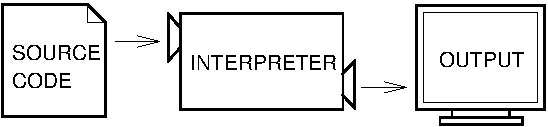
\includegraphics[scale=0.9]{figs/interpret.pdf}}
\caption{Um interpretador processa o programa um pouco de cada vez,
alternadamente ler linhas e executa computações.}
\label{fig.interpret}
\end{figure}

Um compilador lê o programa e o traduz completamente antes de o
programa começa a rodar. Neste contexto, o programa de alto nível é
o chamado de {\bf código fonte}, e o programa traduzido é chamado o
{\bf código objeto} ou {\bf executável}. Uma vez que um programa é
compilado você pode executá-lo repetidamente, sem nova tradução.
Figura~\ref{fig.compile} mostra a estrutura de um compilador.

\begin{figure}
\centerline
{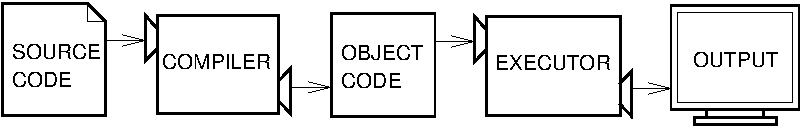
\includegraphics[scale=0.9]{figs/compile.pdf}}
\caption{Um compilador traduz o código fonte em código objeto, o qual é
rodado por um hardware executor.}
\label{fig.compile}
\end{figure}

Python é considerada uma linguagem interpretada, porque os programas desta linguagem
são executados por um interpretador. Há duas maneiras de usar o
interpretador: {\bf modo interativo} e {\bf modo script}. No
modo interativo, você digita os programas em Python e o interpretador exibe
o resultado:
\index{modo interativo}
\index{modo de script}

\begin{verbatim}
>>> 1 + 1
2
\end{verbatim}
%
A tripla bifurcação, \verb">>>", é o sinal de prontidão ou
{\bf prompt} que o interpretador utiliza para indicar que ele está pronto. Se
você digitar {\tt 1 + 1}, o interpretador responde {\tt 2}.
\index{prompt}
\index{sinal de prontidão}

Como alternativa, você pode armazenar o código em um arquivo e usar o interpretador para
executar o conteúdo do arquivo, que é chamado de {\bf script}. Por
convenção os scripts Python têm nomes que terminam com {\tt .py}.
\index{script}

Para executar o script, você tem que dizer ao interpretador o nome do
o arquivo. Se você tem um script chamado {\tt dinsdale.py} e você está
trabalhando em uma janela de comandos UNIX, você digita {\tt python
dinsdale.py}. Em outros ambientes de desenvolvimento, os detalhes
scripts de execução são diferentes. Você pode encontrar instruções para
seu ambiente no site do Python \url{http://python.org.br}.
\index{modo interativo!teste}

Operando no modo interativo é conveniente para testar pequenos pedaços de
código, pois você pode digitar e executá-los imediatamente. Mas para
qualquer coisa maior do que algumas linhas, você deve salvar o seu código
como um script para que você possa modificar e executá-lo no futuro.


\section{O que é um programa?}

Um {\bf programa} é uma seqüência de instruções que especifica como
realizar uma computação. A computação pode ser algo
matemático, como solucionar um sistema de equações ou encontrar a
raízes de uma polinomial, mas também pode ser uma computação simbólica, tais
como busca e substituição de texto em um documento ou (por estranho que seja)
compilar um programa.
\index{programa}

Os detalhes são diferentes em diferentes linguagens, mas algumas instruções
básicas estão presentes em quase todas as linguagens:

\begin{description}

\item[entrada:] Obter dados do teclado, de um arquivo, ou de algum
outro dispositivo.

\item[saída:] Exibir dados na tela ou enviar dados para um
arquivo ou outro dispositivo.

\item[matemática]: Executar operações matemáticas básicas, como adição e
multiplicação.

\item[execução condicional:] Verificar certas condições e
executar o código apropriado.

\item[repetição]: Executar alguma ação repetidamente, normalmente com
alguma variação.

\end{description}

Acredite ou não, isso é praticamente tudo o que existe. Todo
programa que você já usou, não importa quão complicado, é composto de
instruções que se parecem muito com essas mostradas. Então você pode pensar
a programação como o processo de dividir uma tarefa grande e complexa
em subtarefas cada vez menores até que as subtarefas sejam
suficientemente simples para serem realizadas com uma dessas instruções básicas.
\index{algoritmo}

Isso pode ser um pouco vago, mas nós voltaremos a este tópico
quando falarmos de {\bf algoritmos}.

\section{O que é depuração?}
\index{depuração}
\index{falha}
\index{bug}

A programação é propícia a erros. Por capricho, erros de programação
são chamados de {\bf bugs} e o processo de rastreá-los é chamado
{\bf depuração}.
\index{depuração}
\index{bug}

Três tipos de erros podem ocorrer em um programa: erros de sintaxe, erros
em tempo de execução, e erros de semântica. É útil
distingui-los, a fim de encontrá-los mais rapidamente.

\subsection{Erros de sintaxe}
\index{erro de sintaxe}
\index{sintaxe!erro de}
\index{mensagem de erro}

Python só pode executar um programa se a sintaxe for
correta, caso contrário, o interpretador exibe uma mensagem de erro.
{\bf Sintaxe} se refere à estrutura de um programa e as regras sobre
essa estrutura.
Por exemplo, os parênteses têm que vir em pares, de modo que
{\tt (1 + 2)} é válido, mas {\tt 8)} é um {\bf erro de sintaxe}.
\index{sintaxe}
\index{parênteses!correspondência entre}
\index{sintaxe}
\index{cummings, e. e.}

Na línguagem escrita, os leitores podem tolerar a maioria dos erros de sintaxe, ao qual é por isso que
podemos ler a poesia de e. e. cummings sem cuspir mensagens de erro.
Python não é tão tolerante. Se houver um único erro de sintaxe
em qualquer lugar em seu programa, o Python vai exibir uma mensagem de erro, ele para
e você não será capaz de executar o programa. Durante as primeiras
semanas de sua carreira como programador, você provavelmente vai gastar um monte de
tempo procurando erros de sintaxe. A medida que você ganha experiência, você
cometerá menos erros e vai encontrá-los mais rapidamente.

\subsection{Erros em tempo de execução}
\label{tempo de execução}

O segundo tipo de erro é o erro em tempo de execução. Ele é assim chamado porque o
erro não aparece até que o programa tenha iniciado a execução.
Estes erros também são chamados de {\bf exceções}, porque eles normalmente
indicam que algo excepcional (e ruim) aconteceu.
\index{erro em tempo de execução}
\index{em temppo de execução!erro}
\index{exceção}
\index{linguagem segura}
\index{seguro!língua}

Erros de execução são raros em programas simples os quais você vai ver nos
primeiros capítulos, por isso pode demorar um pouco até você encontrar um destes erros.


\subsection{Erros semânticos}
\index{semântica}
\index{erro de semântica}
\index{Semântica!erro}
\index{mensagem de erro}

O terceiro tipo de erro é o {\bf erro de semântica}. Se houver um
erro de semântica em seu programa, ele será executado com sucesso no sentido
que o computador não vai gerar nenhuma mensagem de erro, mas ele
não fará a coisa certa. Ele vai fazer alguma outra coisa. Especificamente, ele
vai fazer o que você disse para ele fazer.

O problema é que o programa que você escreveu não é o programa que você
queria escrever. O significado do programa (sua semântica) está errado.
Identificar erros semânticos pode ser complicado, porque isso exige que você trabalhe
inversamente, olhando a saída do programa e tentando descobrir
o que ele está fazendo.

\subsection{Depuração experimental}

Uma das habilidades mais importantes que você vai adquirir é a de depurar.
Embora possa ser frustrante, depurar é uma das
mais intelectualmente ricas, desafiadoras e interessantes partes da
programação.
\index{depuração experimental}
\index{experimental!depuração}

Em alguns aspectos, a depuração é como um trabalho de detetive. Você se depara
com pistas e você tem que deduzir os processos e eventos que levam
aos resultados que você vê.

Depuração é também como uma ciência experimental. Uma vez que você tem uma ideia
sobre o que está acontecendo de errado, você modifica o seu programa e tenta novamente. Se
sua hipótese estivor correta, então você pode prever o resultado da
modificação e dar um passo mais perto de um programa funcional. Se
sua hipótese estiver errada, você tem que aparecer com uma nova. Como
Sherlock Holmes assinalou, ``Quando você tiver eliminado o
impossível, tudo que resta, embora improvável, deve ser a verdade.''
(A. Conan Doyle, {\em O Signo dos Quatro})
\index{Holmes, Sherlock}
\index{Doyle, Arthur Conan}

Para algumas pessoas, programação e depuração são a mesma coisa. Que
seja, a programação é o processo de gradualmente depurar um programa, até
ele faz o que você quer. A idéia é que você deve começar com uma
programa que não {\em alguma coisa} e fazer pequenas modificações,
depurando-los como você ir, de modo que você sempre tem um programa de trabalho.

Por exemplo, o Linux é um sistema operacional que contém milhares de
linhas de código, mas começou como um programa simples Linus Torvalds
usado para explorar o chip Intel 80386. De acordo com Larry Greenfield,
`` Um dos primeiros projetos de Linus Torvalds foi um programa que deveria alternar
entre imprimir AAAA e BBBB. Isso depois evoluiu para Linux''.
({\Em dos Usuários de Linux Guia} Versão Beta 1).
\index{Linux}

Os últimos capítulos vai fazer mais sugestões sobre depuração e outras
práticas de programação.


\section{linguagens formais e naturais}
\index{linguagem formal}
\index{linguagem natural}
\index{língua! Formais}
\index{língua! Naturais}

{\bf línguas naturais} são as línguas pessoas falam,
como o Inglês, Espanhol e Francês. Eles não foram projetados
por pessoas (embora as pessoas tentem colocar alguma ordem nelas);
eles evoluíram naturalmente.

{\bf linguagens formais} são linguagens que foram projetadas por pessoas para
aplicações específicas. Por exemplo, a notação que matemáticos
uso é uma linguagem formal, que é particularmente bom em denotação
relações entre números e símbolos. Os químicos usam formal
língua para representar a estrutura química de moléculas. E
o mais importante:

\begin{quote}
{Linguagens de programação \bf são linguagens formais que foram
projetado para expressar computações.}
\end{quote}

As linguagens formais tendem a ter regras estritas quanto à sintaxe. Por exemplo,
$ 3 + 3 = 6 $ é uma expressão matemática sintaticamente correta, mas 
$ 3 + = 3 \mbox {\$} 6 $ não é.
$ $ H_2O é um sintaticamente correto
fórmula química, mas _2Zz $ $ não é.

As regras de sintaxe são de dois tipos, pertencentes a {fichas \bf} e
estrutura. Tokens são os elementos básicos da linguagem, tais como
palavras, números e elementos químicos. Um dos problemas com
$ 3 + = 3 \mbox {\$} 6 $ é que \(\$ \) não é um sinal legal em matemática
(Pelo menos até onde eu sei). Da mesma forma, _2Zz $ $ não é legal porque
não há nenhum elemento com a abreviatura $ Zz $.
\index{símbolo}
\index{estrutura}

O segundo tipo de regra sintaxe está relacionado com a estrutura de um
declaração, ou seja, a forma como os sinais são organizados. A declaração
$ 3 + $ = 3 é ilegal porque, embora $ + $ e $ $ = são
fichas legais, você não pode ter um logo após o outro. Da mesma forma,
em uma fórmula química o índice vem após o nome do elemento, não
antes.

\begin{} exercício

Escrever um Inglês bem estruturado
sentenciar com tokens inválidos nele. Em seguida, escreva outra frase
com todos os tokens válidos, mas com estrutura inválida.

\end{} exercício

Quando você lê uma frase em Inglês ou uma declaração formal em
língua, você tem que descobrir o que a estrutura da frase é
(Embora em uma linguagem natural que você faça isso inconscientemente). Este
processo é chamado {\bf análise}.
\index{} parse

Por exemplo, quando você ouve a frase, `` A ficha caiu'', você
compreender que `` o último centavo'' é o tema e `` caiu'' é o
predicado. Depois de ter analisado uma frase, você pode descobrir o que
significado, ou a semântica da frase. Supondo que você sabe
o que um centavo é eo que significa a cair, você vai entender a
implicação geral desta frase.

Embora as linguagens formais e naturais têm muitas características em
comum --- tokens, estrutura, sintaxe e semântica --- há alguns
diferenças:
\index{ambigüidade}
\index{redundância}
\index{} literalidade

\begin{description}

\item[ambigüidade:] linguagens naturais estão cheias de ambiguidade, que
pessoas contornam usando pistas contextuais e outras informações.
As linguagens formais são desenvolvidas para serem quase ou totalmente sem ambiguidade,
o que significa que qualquer declaração tem exatamente um significado,
independentemente do contexto.

\item[redundância:] A fim de compensar a ambigüidade e reduzir
incompreensões, as línguas naturais empregam muita
redundância. Como resultado, eles são muitas vezes prolixo. Linguagens formais
são menos redundantes e mais concisas.

\item[literalidade:] linguagens naturais estão cheias de expressões idiomáticas e metáforas.
Se eu disser: `` A ficha caiu'', provavelmente não há centavo e
nada caindo (este idioma significa que alguém percebeu que algo
após um período de confusão). Linguagens formais
significa exatamente o que eles dizem.

\end{description}

Pessoas que crescem falando uma linguagem natural --- todos --- muitas vezes têm um
tempo para adaptar às linguagens formais. De certa forma, a diferença
entre linguagens formais e naturais é como a diferença entre
poesia e prosa, mas mais ainda:
\index{poesia}
\index{} prosa

\begin{description}

\item[Poesia:] As palavras são usadas pela sua sonoridade, bem como para
o seu significado, e todo o poema, cria um efeito ou
resposta emocional. A ambigüidade não é apenas comum, mas muitas vezes
deliberada.

\item[Prosa:] O significado literal das palavras é mais importante,
e a estrutura contribui mais significado. Prosa é mais fácil para
análise do que a poesia, mas ainda muitas vezes ambígua.

\item[Programas]: O significado de um programa de computador é exato
e literal, e pode ser inteiramente compreendida pela análise do
tokens e estrutura.

\end{description}

Aqui estão algumas sugestões para programas de leitura (e outros formais
línguas). Em primeiro lugar, lembre-se que linguagens formais são muito mais densas
de línguas naturais, por isso leva mais tempo para lê-los. Além disso, o
estrutura é muito importante, por isso geralmente não é uma boa idéia para ler
de cima para baixo, da esquerda para a direita. Em vez disso, aprenda a analisar o
programa em sua cabeça, identificando os tokens e interpretando o
estrutura. Finalmente, os detalhes são importantes. Pequenos erros na
ortografia e pontuação, o que você pode ir longe
nas linguagens naturais, podem fazer uma grande diferença em um formais
língua.


\section{O primeiro programa}
\label{Olá}
\index{Olá, Mundo}

Tradicionalmente, o primeiro programa que você escreve em um novo idioma
é chamado de `` Olá, mundo!'' porque tudo que faz é exibir o
palavras `` Olá, mundo!''. Em Python, ele se parece com isso:

\begin{verbatim}
imprimir "Olá, mundo!"
\end{verbatim}
%
Este é um exemplo de uma {\bf impressão instrução}, que
na verdade não imprimir nada no papel. Ele exibe um valor na
tela. Neste caso, o resultado é as palavras

\begin{verbatim}
Olá, mundo!
\end{verbatim}
%
As aspas no programa marcam o início eo final
do texto a ser exibido, pois eles não aparecem no resultado.
\index{aspas}
\index{declaração print}
\index{declaração! Print}

Em Python 3, a sintaxe para impressão é um pouco diferente:

\begin{verbatim}
print ('Olá, Mundo!')
\end{verbatim}
%
Os parênteses indicam que {\tt print} é uma função. Nós vamos chegar
para funções no capítulo ~ \ref {} funcchap.
\index{função} \{} função de impressão de índice \index {Python 3}

Para o resto deste livro, eu vou usar a instrução de impressão. Se você
está usando Python 3, você terá que traduzir. Mas diferente do
que, há muito poucas diferenças que nós temos que se preocupar.


\section{} Depuração
\index{depuração}

É uma boa idéia para ler este livro em frente a um computador para que você possa
experimentar os exemplos que você vá. Você pode executar a maioria dos exemplos em
modo interativo, mas se você colocar o código em um script, é mais fácil
para experimentar variações.

Sempre que você está experimentando com um novo recurso, você deve tentar
para cometer erros. Por exemplo, no programa `` Olá, mundo!''
o que acontece se você deixar de fora uma das aspas? O que
se você deixar de fora os dois? E se se escreve {\tt print} errado?
\index{mensagem de erro}

Esse tipo de experiência ajuda a lembrar o que você lê, mas também ajuda
com a depuração, porque você começa a conhecer o que significa que as mensagens de erro.
É melhor cometer erros agora e de propósito do que mais tarde
e acidentalmente.

Programação e, especialmente, a depuração, por vezes, traz forte
emoções. Se você está lutando com um bug difícil, você pode
sentir raiva, desanimado ou envergonhado.

Há evidências de que as pessoas naturalmente responder aos computadores como se
eram pessoas. Quando eles trabalham bem, pensamos
deles como companheiros de equipe, e quando eles são obstinados ou rude, nós
respondê-las da mesma maneira como respondemos a rude,
pessoas obstinadas (Reeves e Nass, {\it A mídia
    Equação: como as pessoas tratam Computadores, televisão e novas mídias
    Como o Real People and Places}).
\index{depuração resposta! Emocional}
\index{depuração emocional}

Preparar-se para estas reações podem ajudá-lo a lidar com eles.
Uma abordagem é pensar no computador como um funcionário com
alguns pontos fortes, como a velocidade e precisão, e
fraquezas particulares, como a falta de empatia e de incapacidade
de compreender o quadro geral.

Seu trabalho é ser um bom gerente: encontrar maneiras de tirar proveito
dos pontos fortes e minimizar os pontos fracos. E encontrar maneiras
usar suas emoções para se envolver com o problema,
sem deixar que suas reações interferir com a sua capacidade
para trabalhar de forma eficaz.

Aprender a depuração pode ser frustrante, mas é uma valiosa habilidade
que é útil para muitas atividades além de programação. No
final de cada capítulo, há uma seção de depuração, como este,
com meus pensamentos sobre a depuração. Espero que ajude!


\section{} Glossário

\begin{description}

\item[A resolução de problemas:] artigo O processo de formulação de um problema, encontrar
uma solução, e expressando a solução.
\index{} resolução de problemas

\item[linguagem de alto nível:] A linguagem de programação como Python que
é projetado para ser fácil para os seres humanos a ler e escrever.
\index{linguagem de alto nível}

\item[linguagem de baixo nível:] A linguagem de programação que é projetado
ser fácil para um computador para executar; também conhecido como `` linguagem de máquina'' ou
`` Linguagem assembly.''
\index{linguagem de baixo nível}

\item[a portabilidade]: Uma propriedade de um programa que pode ser executado em mais
de um tipo de computador.
\index{} portabilidade

\item[interpretar]: Para executar um programa em uma linguagem de alto nível
, traduzindo-a uma linha de cada vez.
\index{interpretar}

\item[compilar:] Para traduzir um programa escrito em uma linguagem de alto nível
em uma linguagem de baixo nível de uma só vez, em preparação para posterior
execução.
\index{} compilar

\item[Código fonte:] item de um programa em uma linguagem de alto nível antes
sendo compilada.
\{Código fonte} índice

\item[Código objeto:] Item A saída do compilador, depois que se traduz
o programa.
\index{código objeto}

\item[executável:] Um outro nome para código objeto que está pronto
para ser executado.
\index{executável}

\item[prompt:] caracteres exibidos pelo interpretador para indicar
que está pronto para receber a entrada do usuário.
\index{indicador}

\item[script:] Um programa armazenado em um arquivo (normalmente um que será
interpretado).
\index{} roteiro

\item[modo interativo:] Uma maneira de usar o interpretador Python por
digitar os comandos e expressões no prompt.
\index{modo interativo}

\item[Modo de script:] Uma maneira de usar o interpretador Python para ler
e executar instruções em um script.
\index{modo de script}

\item[programa]: Um conjunto de instruções que especifica uma computação.
\index{programa}

\item[algoritmo:] Um processo geral para a resolução de uma categoria de
problemas.
\index{algoritmo}

\item[bug]: Um erro em um programa.
\index{bug}

\item[depuração:] O processo de encontrar e remover qualquer um dos
três tipos de erros de programação.
\index{depuração}

\item[sintaxe:] A estrutura de um programa.
\index{} sintaxe

\item[erro de sintaxe:] Um erro em um programa que faz com que seja impossível
para analisar (e, portanto, impossível de interpretar).
\index{erro de sintaxe}

\item[exceção:] Um erro que é detectado enquanto o programa está sendo executado.
\index{exceção}

\item[semântica:] O significado de um programa.
\index{} semântica

\item[erro de semântica:] Um erro em um programa que o leva a fazer algo
além do que o programador pretendido.
\index{erro de semântica}

\item[linguagem natural:] Qualquer uma das línguas que as pessoas falam que
evoluiu naturalmente.
\index{linguagem natural}

\item[linguagem formal:] Qualquer uma das línguas que as pessoas projetaram
para fins específicos, tais como a representação de idéias matemáticas ou
programas de computador; todas as linguagens de programação são linguagens formais.
\index{linguagem formal}

\item[token:] Um dos elementos básicos da estrutura sintática de
um programa, análogo a uma palavra em uma língua natural.
\index{símbolo}

\item[análise]: Examinar um programa e analisar a estrutura sintática.
\index{} parse

\item[Declaração print:] item de uma instrução que faz com que o Python
intérprete para exibir um valor na tela.
\index{declaração print}
\index{declaração! Print}


\end{description}


\section{Exercícios}

\begin{} exercício

Use um navegador da web para ir para o site Python \url{http://python.org}.
Esta página contém informações sobre Python e as ligações
para páginas relacionadas com o Python, e dá-lhe a capacidade de pesquisar
a documentação do Python.

Por exemplo, se você digitar {\tt print} na janela de pesquisa, o
primeiro link que aparece é a documentação do {\tt print}
comunicado. Neste ponto, nem tudo vai fazer sentido para você,
mas é bom saber onde ele está.
\index{} documentação
\index{} python.org

\end{} exercício

\begin{} exercício

Inicie o interpretador Python e tipo {\ttajuda()} para iniciar a linha
ajudar a utilidade. Ou você pode digitar \verb"help('print')" para obter informações
sobre o {\tt print} comunicado.

Se este exemplo não funciona, você
pode precisar instalar a documentação Python adicional ou definir uma
variável de ambiente; os detalhes dependem de seu sistema operacional e
versão do Python.
\index{utilitário ajuda}

\end{} exercício

\begin{} exercício

Inicie o interpretador Python e usá-lo como uma calculadora.
Sintaxe do Python para operações matemáticas é quase o mesmo que
notação matemática padrão. Por exemplo, os símbolos
{\tt +}, {\tt -} e {\tt /} denotam adição, subtração
e divisão, como seria de esperar. O símbolo para
multiplicação é {\tt *}.

Se você executar uma corrida de 10 km em 43 minutos e 30 segundos, o que é seu
tempo médio por quilômetro? Qual é a sua velocidade média em milhas por hora?
(Dica: há 1,61 km em uma milha).
\index{calculadora}
\index{ritmo execução}

\end{} exercício




\chapter{Variáveis, expressões e comandos}

\section{Valores e tipos}
\index{value}
\index{type}
\index{string}

A {value \bf} é uma das coisas básicas de um programa trabalha,
como uma carta ou um
número. Os valores que temos visto até agora
são {\tt 1}, {\tt 2}, e
\verb"'Olá, mundo!'".

Estes valores pertencem a diferentes tipos {\bf}:
{\tt 2} é um número inteiro, e \verb "" Olá, mundo! "É uma seqüência {\bf},
assim chamado porque ele contém um `` string'' de letras.
Você (eo interpretador) consegue identificar
cordas, porque eles estão entre aspas.
\index{aspas}

Se você não tiver certeza do tipo de um determinado valor, o intérprete pode dizer.

\begin{verbatim}
>>> Type ('Olá, Mundo!')
<type'str'>
>>> Type (17)
<type'int'>
\end{verbatim}
%
Não é de surpreender, cordas pertencem ao tipo {\tt str} e
inteiros pertencem ao tipo {\tt int}. Menos obviamente, números
com um ponto decimal pertencem a um tipo chamado {\tt flutuador},
porque estes números são representados numa
formato chamado {\bf-ponto flutuante}.
\index{type}
\index{type string}
\index{type! Str}
\{Type} int index
\index{type! Int}
\index{tipo float}
\{!} Flutuador tipo índice

\begin{verbatim}
>>> Type (3.2)
<type'float'>
\end{verbatim}
%
O que dizer de valores como \verb "'17 '" e \verb "0,2 '3'"?
Eles parecem números, mas estão entre aspas, como
strings.
\index{aspas}

\begin{verbatim}
>>> Type ('17 ')
<type'str'>
>>> Type ('3 .2 ')
<type'str'>
\end{verbatim}
%
Eles são strings.

Quando você digitar um número grande, que você pode ser tentado a usar vírgulas
entre grupos de três dígitos, como em {\tt 1.000.000}. Este não é um
integer legal em Python, mas é legal:

\begin{verbatim}
>>> 1.000.000
(1, 0, 0)
\end{verbatim}
%
Bem, isso não é o que esperava! Interpreta Python {\tt
  1000000} como uma seqüência de números inteiros separados por vírgula.
Este é o primeiro exemplo que vemos de um erro de semântica: o código
roda sem produzir uma mensagem de erro, mas ele não faz o
`` Coisa certa.''
\index{erro de semântica}
\index{erro! Semântica}
\index{mensagem de erro}



\section{Variáveis}
\label{variáveis}
\index{variável}
\index{declaração de atribuição}
\index{declaração! Atribuição}

Uma das características mais poderosas de uma linguagem de programação é a
habilidade de manipular variáveis ​​{\bf}. Uma variável é um nome que
refere-se a um valor.

Um {\bf atribuição declaração} cria novas variáveis ​​e dá
elas valores:

\begin{verbatim}
>>> Mensagem = 'E agora para algo completamente diferente'
N = 17 >>>
>>> Pi = 3,1415926535897932
\end{verbatim}
%
Este exemplo faz três atribuições. O primeiro atribui uma string
para uma nova variável chamada {\tt mensagem};
o segundo dá o inteiro {\tt 17} para {\tt n}, o terceiro
atribui o valor (aproximado) de $ \pi $ a {\tt pi}.
\index{diagrama de estado}
\index{diagrama! Estado}

Uma maneira comum de representar variáveis ​​no papel é escrever o nome com
uma seta apontando para o valor da variável. Este tipo de figura é
chamado de diagrama de estado {\bf} porque mostra em que estado cada um dos
variáveis ​​está (pense nisso como o estado da variável da mente).
Figura ~ \ref {fig.state2} mostra o resultado do exemplo anterior.

\begin{figure}
\centerline
{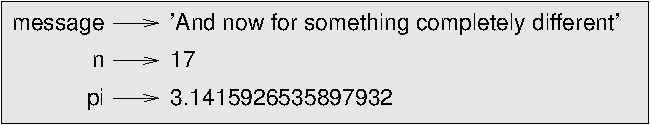
\includegraphics[scale = 0.8] {figs/state2.pdf}}
\caption{Diagrama de Estado.}
\label{} fig.state2
\end{figure}

O tipo de uma variável é o tipo do valor que se refere.

\begin{verbatim}
>>> Type (mensagem)
<type'str'>
>>> Type (n)
<type'int'>
>>> Type (pi)
<type'float'>
\end{verbatim}

\begin{} exercício

Se você digitar um número inteiro com um zero à esquerda, você pode obter
um erro confuso:

\begin{verbatim}
>>> CEP = 02492
                  ^
SyntaxError: símbolo inválido
\end{verbatim}

Outros números parecem funcionar, mas os resultados são bizarros:

\begin{verbatim}
>>> CEP = 02132
>>> CEP
1114
\end{verbatim}

Você pode descobrir o que está acontecendo? Dica: exibir o
valores {\tt 01}, {\tt 010}, {\tt 0100} e {\tt 01000}.
\index{octal}

\end{} exercício



\section{Nomes de variáveis ​​e palavras-chave}
\index{palavra-chave}

Os programadores geralmente escolhem nomes para suas variáveis ​​que
são significativos --- eles documentam o que a variável é utilizada.

Os nomes das variáveis ​​podem ser arbitrariamente longos. Eles podem conter
letras e números, mas eles têm que começar com uma letra.
É legal usar letras maiúsculas, mas é uma boa idéia
para começar os nomes de variáveis ​​com uma letra minúscula (você
ver por que mais tarde).

O caractere sublinhado, \verb "_", pode aparecer em um nome.
Ele é frequentemente usado em nomes com múltiplas palavras, como
\Verb "my_name" ou \verb "airspeed_of_unladen_swallow".
\index{caractere sublinhado}

Se você der a uma variável um nome ilegal, você tem um erro de sintaxe:

\begin{verbatim}
>>> 76trombones = 'grande desfile'
SyntaxError: sintaxe inválida
>>> Mais @ = 1000000
SyntaxError: sintaxe inválida
>>> Class = 'Zymurgy Teórica Avançada'
SyntaxError: sintaxe inválida
\end{verbatim}
%
{76trombones \tt} é ilegal porque não começar com uma letra.
{\tt mais @} é ilegal porque contém um caractere ilegal, {\tt
@}. Mas o que há de errado com classe {\tt}?

Acontece que {class \tt} é uma das palavras-chave {\bf} em Python. O
intérprete usa palavras-chave para reconhecer a estrutura do programa,
e eles não podem ser utilizados como nomes de variáveis.
\index{palavra-chave}

Python 2 tem 31 palavras-chave:

\begin{verbatim}
e del por não enquanto    
como elif global, ou com     
afirmar else if rendimento passagem    
quebrar exceto impressão importação              
exec classe em aumento              
continuar finalmente é o retorno             
def para lambda tentativa
\end{verbatim}
%
Em Python 3, {\tt exec} não é mais uma palavra-chave, mas {\tt} não-local é.

Você pode querer manter esta lista acessível. Se o interpretador acusar erro
sobre um de seus nomes de variáveis ​​e você não sabe o porquê, veja se ele
está nesta lista.


\section{Operadores e operandos}
\index{operador, aritmética}
\index{operador aritmético}
\index{operando}
\index{expressão}

{Operadores \bf} são símbolos especiais que representam computações como
adição e multiplicação. Os valores do operador é aplicada
são chamados de {\bf operandos}.

Os operadores {\tt +}, {\tt -}, {\tt *}, {\tt /} e {\tt **}
realizar operações de adição, subtração, multiplicação, divisão e
exponenciação, como nos exemplos a seguir:

\begin{verbatim}
20 32 horas-1 horas * 60 + minuto minute/60 5 ** 2 (5 +9) * (15-7)
\end{verbatim}
%
Em algumas outras línguas, \verb "^" é utilizado para exponenciação, mas
em Python é um operador bit a bit XOR chamado. Eu não cobrirá
operadores bit a bit, neste livro, mas você pode ler sobre
los em \url{http://wiki.python.org/moin/BitwiseOperators}.
\index{operador bit}
\index{operador! Bitwise}

Em Python 2, o operador de divisão pode não fazer o que você espera:

\begin{verbatim}
>>> Minuto = 59
>>> Minute/60
0
\end{verbatim}
%
O valor de {\tt minuto} é de 59 e, em aritmética convencional 59
dividido por 60 é 0,98333, não 0. A razão para a discrepância é
que Python está realizando {chão \bf divisão}.
Quando ambos os operandos são inteiros, o resultado é também uma
inteiros; costeletas divisão andar fora da fração
parte, portanto, neste exemplo, ele arredonda para baixo a zero.

Em Python 3, o resultado desta divisão é uma {float \tt}. O novo operador
{\tt / /} executa divisão chão.
\index{Python 3}
\index{divisão chão}
\index{divisão em ponto flutuante}
\index{divisão! Chão}
\index{divisão! Ponto flutuante}

Se um dos operandos é um número de ponto flutuante, Python realiza
divisão de ponto flutuante, eo resultado é uma {\tt flutuador}:

\begin{verbatim}
>>> Minute/60.0
0,98333333333333328
\end{verbatim}


\section{expressões e declarações}

Um {\bf expressão} é uma combinação de valores, variáveis ​​e operadores.
Um valor por si só é considerado uma expressão, e por isso é
uma variável, então o seguinte são todas expressões legais
(Assumindo que a variável {\tt x} foi atribuído um valor):
\index{expressão}
\index{avaliar}

\begin{verbatim}
17
x
x + 17
\end{verbatim}
%
A declaração {\bf} é uma unidade de código que o interpretador Python pode
executar. Vimos dois tipos de declaração: impressão e
atribuição.

Tecnicamente uma expressão também é uma afirmação, mas é provável que seja
mais simples de pensar neles como coisas diferentes. A diferença importante
é uma expressão que tem um valor, uma declaração não.


\section{modo interativo eo modo de script}

Uma das vantagens de trabalhar com uma linguagem interpretada é que
você pode testar pedaços de código em modo interativo, antes de colocá-los
em um script. Mas há diferenças entre o modo interativo
eo modo de script que pode ser confuso.
\index{modo interativo}
\index{modo de script}

Por exemplo, se você estiver usando o Python como uma calculadora, você pode digitar

\begin{verbatim}
>>> Milhas = 26,2
>>> Milhas * 1,61
42,182
\end{verbatim}

A primeira linha atribui um valor a {\tt quilômetros}, mas não tem visível
efeito. A segunda linha é uma expressão, de modo que o intérprete
avalia e exibe o resultado. Assim, ficamos a saber que uma maratona é
cerca de 42 quilômetros.

Mas se você digitar o mesmo código em um script e executá-lo, você não obter
saída de todo. No modo de script de uma expressão, por si só, não tem
efeito visível. Pitão realmente avalia a expressão, mas não faz
exibir o valor, a menos que você diga a ele:

\begin{verbatim}
milhas = 26,2
impressão milhas * 1,61
\end{verbatim}

Este comportamento pode ser confuso no início.

Um script normalmente contém uma seqüência de instruções. Se houver
é mais do que uma declaração, os resultados aparecem uma de cada vez
como as instruções são executadas.

Por exemplo, o script

\begin{verbatim}
impressão 1
x = 2
print x
\end{verbatim}
%
produz a saída

\begin{verbatim}
1
2
\end{verbatim}
%
O comando de atribuição não produz saída.

\begin{} exercício

Digite as seguintes declarações no interpretador Python para ver
o que eles fazem:

\begin{verbatim}
5
x = 5
x + 1
\end{verbatim}
%
Agora coloque as mesmas instruções em um script e executá-lo. O que
é a saída? Modifique o script, transformando cada
expressão em uma instrução de impressão e, em seguida, executá-lo novamente.
\end{} exercício


\section{Ordem dos operadores}
\index{ordem das operações}
\index{regras de precedência}
\index{} PEMDAS

Quando mais de um operador aparece em uma expressão, a ordem de
avaliação depende das regras {\bf de precedência}. Para
operadores matemáticos, Python segue a convenção matemática.
A sigla {\bf PEMDAS} é uma maneira útil de
lembre-se das regras:
\index{parênteses! Prioridade primordial}

\begin{itemize}

\item{\bf P} arentheses têm a maior prioridade e pode ser usado 
para forçar uma expressão a ser avaliada na ordem que você quiser. Desde
expressões entre parênteses são avaliadas primeiro, {\tt 2 * (3-1)} é 4,
e {\tt (1 1) ** (5-2)} é de 8. Você também pode usar parênteses para fazer uma
expressão mais fácil de ler, como em {\tt (minuto * 100) / 60}, mesmo
se ele não muda o resultado.

\item{\bf E} xponentiation tem a próxima precedência mais alta, por isso,
{\tt 2 ** 1 1} é 3, não 4, e {\tt 3 * 1 ** 3} é 3, não 27.

\item{\bf M} ultiplication e {\bf D} iVision têm a mesma precedência,
que é maior do que o {\bf Um ddition} e {\bf S} ubtraction, que também
têm a mesma precedência. Assim {\tt 2 * 3-1} é 5, não 4, e
{\tt 6 4/2} é de 8, não 5.

\Operadores de itens com a mesma precedência são avaliados da esquerda para
  direito (exceto exponenciação). Assim, na expressão {\graus tt /
    2 * pi}, a divisão ocorre em primeiro lugar e o resultado é multiplicado
  por {\tt pi}. Para dividir por $ 2 \pi $, você pode usar parênteses ou escrever
  {Graus \tt / 2 / pi}.

\end{itemize}

Eu não trabalho muito difícil lembrar de regras de precedência para outros
operadores. Se eu não posso dizer, olhando para a expressão, eu uso
parênteses para tornar mais óbvio.

\{} Operações de corda seção
\index{string! Operação}
\index{operador! String}

Em geral, você não pode executar operações matemáticas em strings, ainda
se as cordas parecem números, então o seguinte são ilegais:

\begin{verbatim}
'2 '- '1' 'Ovos' / 'fácil' terceiro '*' um encanto "
\end{verbatim}
%
O {\tt +} operador trabalha com strings, mas
pode não fazer o que você espera: ele executa
{\bf concatenação}, o que significa juntar as cordas por
ligando-end-to-end. Por exemplo:
\index{concatenação}

\begin{verbatim}
primeiro = 'garganta'
segundo = 'rouxinol'
imprimir primeiro + segundo
\end{verbatim}
%
A saída deste programa é {\tt throatwarbler}.

O {\tt *} operador também trabalha nas cordas, ele realiza repetição.
Por exemplo, \verb "'Spam' * 3" é \verbo "'SpamSpamSpam'." Se um dos operandos
é uma string, o outro tem que ser um número inteiro.

Este uso de {\tt +} e {\tt *} faz sentido por
analogia com adição e multiplicação. Assim como {\tt 4 * 3} é
equivalente a {\tt 4 4 4}, espera-se \verbo "'Spam' * 3" ser a mesma
\Verb "'Spam' + 'Spam' + 'Spam'", e é. Por outro lado, existe uma
forma significativa separa concatenação e repetição são
diferente de adição e multiplicação.
Você pode pensar em uma propriedade que tem adição
que concatenação não?
\index{} comutatividade


\section{Comentários}
\index{comment}

Como os programas de ficar maior e mais complicado, eles ficam mais difíceis
de ler. As linguagens formais são densas, e é muitas vezes difícil de
olhar para um pedaço de código e descobrir o que ele está fazendo, ou o porquê.

Por esta razão, é uma boa idéia para adicionar notas aos seus programas para explicar
em linguagem natural que o programa está fazendo. Estas notas são chamados
{comentários \bf} e eles começam com o verbo símbolo \"#":

\begin{verbatim}
# Calcular a percentagem da hora que tenha decorrido
porcentagem = (minuto * 100) / 60
\end{verbatim}
%
Neste caso, o comentário aparece em uma linha por si só. Você também pode colocar
comentários no final de uma linha:

\begin{verbatim}
percentual = (minuto * 100) / 60 # percentagem de uma hora
\end{verbatim}
%
Tudo, desde o {\tt \#} para o fim da linha é ignorado --- ele
não tem efeito sobre o programa.

Comentários são mais úteis quando eles documentam recursos não-óbvios de
o código. É razoável supor que o leitor pode descobrir
{\Em que} o código faz, é muito mais útil para explicar {\em por que}.

Este comentário é redundante com o código e inútil:

\begin{verbatim}
v = 5 # atribuir 5 a v
\end{verbatim}
%
Esse comentário contém informações úteis que não está no código:

\begin{verbatim}
v = velocidade de 5 # em metros / segundo. 
\end{verbatim}
%
Bons nomes de variáveis ​​podem reduzir a necessidade de comentários, mas
nomes longos podem fazer expressões complexas difíceis de ler, para que haja
uma troca.


\section{} Depuração
\index{depuração}

Neste ponto, o erro de sintaxe que são mais propensos a fazer é
um nome de variável ilegal, como {\tt classe} e {\tt rendimento}, que
são palavras-chave, ou \verb "estranho ~ trabalho" e \verb"US$", que contêm
caracteres ilegais.
\index{erro de sintaxe}
\index{erro! Sintaxe}

Se você colocar um espaço em um nome de variável, Python pensa que é dois
operandos sem um operador:

\begin{verbatim}
>>> Ruim name = 5
SyntaxError: sintaxe inválida
\end{verbatim}
%
Para erros de sintaxe, as mensagens de erro não ajuda muito.
As mensagens mais comuns são {\tt SyntaxError: sintaxe inválida} e
{\tt SyntaxError: invalid token}, nenhum dos quais é muito informativo.
\index{mensagem de erro}
\index{uso antes def}
\index{exceção}
\index{erro de execução}
\index{erro! Runtime}

O erro de execução que são mais propensos a fazer é um `` uso antes
def;'' isto é, tentando usar uma variável antes de atribuir
um valor. Isso pode acontecer se você soletrar um nome errado variável:

\begin{verbatim}
>>> Principal = 327,68
>>> Taxa de juros = princípio *
NameError: name 'princípio' não está definido
\end{verbatim}
%
Nomes de variáveis ​​são case sensitive, então {\tt LaTeX} não é o
mesmo que {\tt látex}.
\index{maiúsculas e minúsculas, os nomes de variáveis}
\index{erro de semântica}
\index{erro! Semântica}

Neste ponto, a causa mais provável de um erro de semântica é
a ordem das operações. Por exemplo, para avaliar
 $ \Frac {1} {2 \pi} $,
você pode ser tentado a escrever

\begin{verbatim}
>>> 1.0 / 2.0 * pi
\end{verbatim}
%
Mas a divisão acontece primeiro, então você receberia US $ \pi / 2 $, que
não é a mesma coisa! Não há nenhuma maneira para Python
para saber o que você quis escrever, então, neste caso, você não
uma mensagem de erro, você só obter a resposta errada.
\index{ordem das operações}


\section{} Glossário

\begin{description}

\item[valor]: Uma das unidades básicas de dados, como um número ou cadeia de caracteres, 
que um programa manipula.
\index{value}

\item[Tipo:] A categoria de valores. Os tipos que temos visto até agora
são inteiros (tipo {\tt int}), números de ponto flutuante (tipo {\tt
flutuam}) e cordas (tipo {\tt str}).
\index{type}

\item[inteiro]: Um tipo que representa números inteiros.
\index{inteiro}

\item[ponto flutuante:] Um tipo que representa números com fração
peças.
\index{ponto flutuante}

\item[string]: Um tipo que representa sequências de caracteres.
\index{string}

\item[variável]: Um nome que se refere a um valor.
\index{variável}

\item[declaração]: A seção de código que representa um comando ou ação. Assim
agora, as declarações que temos visto são as atribuições e instruções de impressão.
\index{declaração}

\item[atribuição]: A instrução que atribui um valor a uma variável.
\index{atribuição}

\item[Diagrama de estado:] item A representação gráfica de um conjunto de variáveis ​​e
valores que se referem.
\index{diagrama de estado}

\item[palavra-chave]: A palavra reservada usada pelo compilador para analisar uma
programa, você não pode usar palavras-chave como {\tt if}, {\tt def} e {\tt enquanto} como
nomes de variáveis.
\index{palavra-chave}

\item[operador]: Um símbolo especial que representa uma computação simples, como
adição, multiplicação ou concatenação.
\index{operador}

\item[operando:] Um dos valores sobre os quais o operador opera.
\index{operando}

\item[Divisão andar:] Item A operação que divide dois números e corta
a parte de fração.
\index{divisão chão}

\item[expressão:] A combinação de variáveis, operadores e valores que
representa um único valor do resultado.
\index{expressão}

\item[avaliar]: Para simplificar uma expressão através da realização de operações
, a fim de se obter um único valor.

\item[regras de precedência:] o conjunto de regras que rege a ordem em que
expressões envolvendo múltiplos operadores e operandos são avaliadas.
\index{regras de precedência}
\index{} precedência

\item[concatenar:] Para participar de dois operandos end-to-end.
\index{concatenação}

\item[Comentário:] Informações em um programa que é destinado a outro
programadores (ou qualquer um que lê o código-fonte) e não tem efeito sobre o
a execução do programa.
\index{comment}

\end{description}


\section{Exercícios}

\begin{} exercício

Suponha que execute os seguintes comandos de atribuição:

\begin{verbatim}
width = 17
height = 12,0
delimitador = '.'
\end{verbatim}

Para cada uma das seguintes expressões, escrever o valor do
expressão e do tipo (o valor da expressão).

\begin{enumerate}

\item{width \tt / 2}

\item{width/2.0 \tt}

\item{height \tt / 3}

\item{\tt 1 + 2 * 5}

\item{\tt delimitador * 5}

\end{enumerate}

Use o interpretador Python para conferir suas respostas.
\end{} exercício

\begin{} exercício

Pratique usando o interpretador Python como uma calculadora: 
\index{calculadora}

\begin{enumerate}

\item O volume de uma esfera com raio $ r $ é $ \frac {4} {3} \pi r ^ 3 $.
  O que é o volume de uma esfera com raio de 5? Dica: 392,7 está errado!

\item Suponha que o preço de capa de um livro é \$ 24,95, mas as livrarias obter um
  40 \de desconto. O custo de envio \$ 3 para a primeira cópia e 75 centavos
  para cada cópia adicional. Qual é o custo total para atacado
  60 cópias?

\item Se eu deixar minha casa às 06:52 e correr uma milha em um ritmo fácil
  (8:15 por quilômetro), então 3 milhas de tempo (7:12 por quilômetro) e 1 milha
  ritmo fácil, novamente, que horas eu chego em casa no café da manhã?
\index{ritmo execução}

\end{enumerate}
\end{} exercício


\chapter{Funções}
\label{} funcchap

\{} Seção Chamadas de função
\label{} functionchap
\index{chamada da função}

No contexto de programação, uma função de {\bf} é uma sequência de chamada
declarações que executa um cálculo. Quando você define uma função,
você especificar o nome ea seqüência de declarações. Mais tarde, você pode
``'' Chamar a função pelo nome.  
Nós já vimos um exemplo de uma {\bf função de chamada}:

\begin{verbatim}
>>> Type (32)
<T ipo 'int'>
\end{verbatim}
%
O nome da função é {type \tt}. A expressão em parênteses
é chamado o argumento {\bf} da função. O resultado, para este
função, é o tipo do argumento.
\index{parênteses! Argumento}

É comum dizer que uma função ``'' leva um argumento e `` retorna''
um resultado. O resultado é chamado de valor de retorno {\bf}.
\index{argumento}
\index{valor de retorno}


\{Funções de conversão de tipo} secção
\index{conversão! Tipo}
\{} Índice de conversão de tipo

De Elkner:
Comentário sobre se estas coisas são _really_ funções?
Usomax como um exemplo de um built-in?

A minha resposta:
Que estão na lista de `` funções embutidas'' assim que eu sou
Dispostos a chamá-los de funções.

Python fornece funções nativas que convertem valores
de um tipo para outro. O {\tt int} function recebe um valor eo
converte para um inteiro, se puder, ou se queixa de outro modo:
\index{função int}
\index{function! Int}

\begin{verbatim}
>>> Int ('32 ')
32
>>> Int ('Olá')
ValueError: Invalid literal para int (): Olá
\end{verbatim}
%
{\tt int} pode converter valores de ponto flutuante para inteiros, mas
não completam, que corta a parte de fração:

\begin{verbatim}
>>> Int (3,99999)
3
>>> Int (-2,3)
-2
\end{verbatim}
%
{\tt flutuador} converte inteiros e strings em ponto flutuante
números:
\index{função de flutuação}
\index{function! Flutuador}

\begin{verbatim}
>>> Float (32)
32,0
>>> Float ('3 0,14159 ')
3,14159
\end{verbatim}
%
Finalmente, {\tt str} converte o argumento para uma string:
\index{função str}
\index{function! Str}

\begin{verbatim}
>>> Str (32)
'32 '
>>> Str (3.14159)
'3 0,14159 '
\end{verbatim}
%



\section{funções matemáticas}
\index{função matemática}
\index{função, matemática}

Python tem um módulo matemático que fornece a maior parte do familiar
funções matemáticas. A {módulo \bf} é um arquivo que contém uma
coleção de funções relacionadas.
\index{módulo}
\index{módulo objeto}

Antes de podermos usar o módulo, temos de importá-lo:

\begin{verbatim}
>>> Matemática importação
\end{verbatim}
%
Esta declaração cria uma {\bf módulo objeto} matemática nomeado. Se
você imprime o objeto módulo, você tem algumas informações sobre ele:

\begin{verbatim}
>>> Print matemática
<module'math' (built-in)>
\end{verbatim}
%
O objeto módulo contém as funções e variáveis ​​definidas no
módulo. Para acessar uma das funções, você tem que especificar o nome
do módulo e o nome da função, separados por um ponto (também
conhecido como um ponto final). Este formato é chamado {\bf dot notação}.
\index{} a notação de ponto

\begin{verbatim}
>>> Ratio = signal_power / noise_power
>>> Decibéis = 10 * math.log10 (razão)

>>> Radianos = 0,7
>>> Height = math.sin (radianos)
\end{verbatim}
%
O primeiro exemplo usa \verb "log10" para computar 
uma relação sinal-para-ruído em decibéis (assumindo que \verbo "signal_power" e
\Verb "noise_power" são definidos). O módulo de matemática também fornece {log \tt},
que calcula logaritmos de base {\tt e}.
\index{função de log}
\index{function! Log}
\index{função seno}
\index{} radiano
\index{função trigonométrica}
\index{function, trigonométricas}

O segundo exemplo encontra o seno de {\tt radianos}. O nome do
variável é um indício de que {\tt pecado} eo outro trigonométricas
funções ({\tt cos}, {\tt bronzeado}, etc) ter argumentos em radianos. Para
converter de graus em radianos, divida por 360 e multiplique por
$ 2 \pi $:

\begin{verbatim}
>>> Graus = 45
>>> radianos = graus / 360,0 * 2 * math.pi
>>> Math.sin (radianos)
0,707106781187
\end{verbatim}
%
A expressão {\tt math.pi} recebe a variável {pi \tt} da matemática
módulo. O valor desta variável é uma aproximação
de $ \pi $, com precisão de cerca de 15 dígitos.
\index{pi}

Se você sabe
sua trigonometria, você pode conferir o resultado anterior, comparando-a
a raiz quadrada de dois, dividido por dois:
\index{função sqrt}
\index{function! Sqrt}

\begin{verbatim}
>>> Math.sqrt (2) / 2.0
0,707106781187
\end{verbatim}
%

\section{Composição}
\index{composição}

Até agora, vimos os elementos de um programa --- variáveis,
expressões e declarações --- isoladamente, sem falar sobre como
combiná-los.

Uma das características mais úteis de linguagens de programação é a sua
capacidade de pegar pequenos blocos e {\bf compor} eles. Para
exemplo, o argumento de uma função pode ser qualquer tipo de expressão,
incluindo operadores aritméticos:

\begin{verbatim}
x = math.sin (graus / 360,0 * 2 * math.pi)
\end{verbatim}
%
E até mesmo chamadas de função:

\begin{verbatim}
x = math.exp (math.log (x +1))
\end{verbatim}
%
Quase em qualquer lugar você pode colocar um valor, você pode colocar um arbitrário
expressão, com uma exceção: o lado esquerdo de uma atribuição
declaração tem que ser um nome de variável. Qualquer outra expressão à esquerda
lado é um erro de sintaxe (veremos exceções a essa regra
mais tarde).

\begin{verbatim}
>>> minuto = horas * 60 # direita
>>> horas * 60 = minutos # errado!
SyntaxError: Não é possível atribuir ao operador
\end{verbatim}
%
\index{} SyntaxError
\index{exceção! SyntaxError}


\section{Adicionando novas funções}

Até agora, só têm vindo a utilizar as funções que vêm com Python,
mas também é possível adicionar novas funções.
A função {\bf definição} especifica o nome de uma nova função e
a seqüência de instruções que são executadas quando a função é chamada.
\index{função}
\index{definição da função}
\{Função definição!} Índice

Aqui está um exemplo:

\begin{verbatim}
print_lyrics DEF ():
    imprimir "Eu sou um lenhador, e eu estou bem."
    imprimir "Eu durmo a noite toda e eu trabalho o dia todo."
\end{verbatim}
%
{\tt def} é uma palavra-chave que indica que esta é uma função
definição. O nome da função é \verb "print_lyrics". O
regras para nomes de funções são as mesmas que para os nomes de variáveis: letras,
números e alguns sinais de pontuação são legais, mas o primeiro caractere
não pode ser um número. Você não pode usar uma palavra-chave como o nome de uma função,
e você deve evitar ter uma variável e uma função com o mesmo
nomear.
\index{palavra-chave def}
\index{palavra-chave! Def}
\index{argumento}

Os parênteses vazios depois do nome indicam que esta função
não leva nenhum argumento.
\index{parênteses! Vazio}
\index{header}
\index{corpo}
\index{recuo}
\index{} cólon

A primeira linha da definição da função é chamada de {\bf cabeçalho};
o resto é chamado o corpo {\bf}. O cabeçalho tem que terminar com dois pontos
e o corpo tem que ser recuado. Por convenção, o recuo é
sempre quatro espaços (veja Seção ~ \ref {editor}). O corpo pode conter
qualquer número de instruções.

As cordas nas instruções de impressão são colocados em dupla
citações. As aspas simples e aspas duplas fazem a mesma coisa;
a maioria das pessoas usar aspas simples, exceto em casos como este, onde
aspas simples (que também é um apóstrofo) aparece na string.
\index{} elipses

Se você digitar uma definição de função no modo interativo, o intérprete
imprime elipses ({\em ...}) para que você saiba que a definição
não está completo:

\begin{verbatim}
>>> Def print_lyrics ():
... imprimir "Eu sou um lenhador, e eu estou bem."
... imprimir "Eu durmo a noite toda e eu trabalho o dia todo."
...
\end{verbatim}
%
Para terminar a função, você tem que digitar uma linha vazia (isto é
não é necessário em um script).

A definição de uma função cria uma variável com o mesmo nome.

\begin{verbatim}
>>> print_lyrics impressão
<function print_lyrics em 0xb7e99e9c>
>>> Type (print_lyrics)
<type'function'>
\end{verbatim}
%
O valor de \verb "print_lyrics" é uma {\bf função de objeto}, que
tem tipo \verb "'função'".
\index{função de objeto}
\index{objeto! Função}

A sintaxe para chamar a nova função é o mesmo que
para funções internas:

\begin{verbatim}
>>> Print_lyrics ()
Eu sou um lenhador, e eu estou bem.
Eu durmo a noite toda e eu trabalho o dia todo.
\end{verbatim}
%
Depois de ter definido uma função, você pode usá-lo dentro de outro
função. Por exemplo, para repetir o refrão anterior, podemos escrever
uma função chamada \verb "repeat_lyrics":

\begin{verbatim}
repeat_lyrics DEF ():
    print_lyrics ()
    print_lyrics ()
\end{verbatim}
%
E em seguida, chamar \verb "repeat_lyrics":

\begin{verbatim}
>>> Repeat_lyrics ()
Eu sou um lenhador, e eu estou bem.
Eu durmo a noite toda e eu trabalho o dia todo.
Eu sou um lenhador, e eu estou bem.
Eu durmo a noite toda e eu trabalho o dia todo.
\end{verbatim}
%
Mas isso não é realmente como diz a canção.


\section{Definições e usos}
\index{definição da função}

Reunindo os fragmentos de código da seção anterior, o
programa completo fica assim:

\begin{verbatim}
print_lyrics DEF ():
    imprimir "Eu sou um lenhador, e eu estou bem."
    imprimir "Eu durmo a noite toda e eu trabalho o dia todo."

repeat_lyrics DEF ():
    print_lyrics ()
    print_lyrics ()

repeat_lyrics ()
\end{verbatim}
%
Este programa contém duas definições de funções: \verb "print_lyrics" e
\verb "repeat_lyrics". Definições de funções são executadas como quaisquer outros
declarações, mas o efeito é criar objetos de função. As demonstrações
dentro da função não são executados até que a função é chamada, e
a definição da função não gera nenhuma saída.
\index{uso antes def}

Como você poderia esperar, você tem que criar uma função antes de poder
executá-lo. Em outras palavras, a definição de função tem que ser
executado antes da primeira vez que é chamado.

\begin{} exercício

Mova a última linha deste programa
para o topo, de modo que a chamada de função aparece antes das definições. Corrida
o programa e ver o erro
mensagem que você recebe.

\end{} exercício

\begin{} exercício

Mova a chamada de função de volta para o fundo
e mova a definição de \verb "print_lyrics", após a definição de
\verb "repeat_lyrics". O que acontece quando você executar este programa?

\end{} exercício


\section{fluxo de execução}
\index{fluxo de execução}

A fim de assegurar que uma função é definida antes da sua primeira utilização,
você tem que saber a ordem em que os comandos são executados, o que é
chamado de fluxo {\bf de execução}.

Execução sempre começa com a primeira instrução do programa.
Os comandos são executados um de cada vez, em ordem de cima para baixo.

As definições de função não alteram o fluxo de execução do
programa, mas lembre-se que comandos dentro da função não são
executado até que a função é chamada.

Uma chamada de função é como um desvio no fluxo de execução. Em vez de
ir para o próximo comando, o fluxo salta para o corpo de
a função, executa todos os comandos lá, e depois volta
para pegar de onde parou.

Isso soa bastante simples, até que você lembre-se que uma função pode
chamar outro. Enquanto no meio de uma função, o programa poderia
tem que executar as instruções em outra função. Mas enquanto
executar essa nova função, o programa poderia ter de executar ainda
outra função!

Felizmente, Python é bom em manter o controle de onde ele está, para que cada
vez que uma função se completa, o programa retoma de onde parou em
a função que o chamou. Quando se chega ao final do programa,
ele termina.

Qual é a moral deste conto sórdido? Quando você lê um programa, você
nem sempre quer ler de cima para baixo. Às vezes faz
mais sentido se você seguir o fluxo de execução.


\section{Parâmetros e argumentos}
\label{parâmetros}
\index{parâmetro}
\index{parâmetro de função}
\index{argumento}
\index{argumento da função}

Algumas das funções internas que temos visto requerem argumentos. Para
exemplo, quando você chamar {\tt math.sin} você passar um número
como um argumento. Algumas funções recebem mais de um argumento:
{\tt math.pow} preciso dois, a base eo expoente.

Dentro da função, os argumentos são atribuídos aos
variáveis ​​chamadas parâmetros {\bf}. Aqui é um exemplo de um
função definida pelo usuário que recebe um argumento:
\index {parênteses! parâmetros}

\begin{verbatim}
def print_twice (bruce):
    imprimir bruce
    imprimir bruce
\end{verbatim}
%
Esta função atribui o argumento para um parâmetro
chamado {\tt bruce}. Quando a função é chamada, ela imprime o valor de
o parâmetro (seja ele qual for) duas vezes.

Esta função funciona com qualquer valor que pode ser impresso.

\begin{verbatim}
>>> Print_twice ('Spam')
Spam
Spam
>>> Print_twice (17)
17
17
>>> Print_twice (math.pi)
3,14159265359
3,14159265359
\end{verbatim}
%
As mesmas regras de composição que se aplicam a funções nativas também
se aplicam às funções definidas pelo usuário, de modo que podemos usar qualquer tipo de expressão
como um argumento para \verb "print_twice":
\index{composição}

\begin{verbatim}
>>> Print_twice ('Spam' * 4)
Spam Spam
Spam Spam
>>> Print_twice (math.cos (math.pi))
-1.0
-1.0
\end{verbatim}
%
O argumento é avaliado antes que a função é chamada, por isso,
nos exemplos as expressões \verbo "'Spam' * 4" e
{\tt math.cos (math.pi)} só são avaliados uma vez.
\index{argumento}

Você também pode usar uma variável como argumento:

\begin{verbatim}
>>> Michael = 'Eric, a metade de uma abelha. "
>>> Print_twice (michael)
Eric, a metade de uma abelha.
Eric, a metade de uma abelha.
\end{verbatim}
%
O nome da variável que passamos como um argumento ({\tt michael}) tem
nada a ver com o nome do parâmetro ({\tt bruce}). Ele
Não importa o que o valor foi chamado de volta para casa (em que o chamador);
aqui em \verb "print_twice", chamamos todo mundo {\tt bruce}.


\section {Variáveis ​​e parâmetros são locais}
\index{variável local}
\index{variável! Locais}

Quando você cria uma variável dentro de uma função, é {\bf locais},
o que significa que somente
existe dentro da função. Por exemplo:
\index {parênteses! parâmetros}

\begin{verbatim}
cat_twice def (parte1, parte2):
    cat = parte1 + parte2
    print_twice (cat)
\end{verbatim}
%
Esta função recebe dois argumentos, concatena-los, e imprime
o resultado duas vezes. Aqui está um exemplo que usa-lo:
\index{concatenação}

\begin{verbatim}
>>> Linha1 = 'Bing Tiddle'
>>> Linha2 = 'estrondo Tiddle.
>>> Cat_twice (linha1, linha2)
Bing Tiddle Tiddle estrondo.
Bing Tiddle Tiddle estrondo.
\end{verbatim}
%
Quando \verb "cat_twice" termina, a variável {\tt gato}
é destruído. Se tentarmos imprimi-lo, temos uma exceção:
\index{} NameError
\index{exceção! NameError}

\begin{verbatim}
>>> Gato impressão
NameError: name 'gato' não está definido
\end{verbatim}
%
Os parâmetros também são locais.
Por exemplo, fora \verbo "print_twice", não há nenhuma
tal coisa como {\tt bruce}.
\index{parâmetro}


\section{Diagramas de pilha}
\label{} stackdiagram
\index{diagrama de pilha}
\index{função frame}
\index{frame}

Para manter o controle de quais variáveis ​​podem ser usadas aonde, às vezes é
útil para desenhar uma {\bf pilha diagrama}. Como diagramas de estado, pilha
diagramas mostram o valor de cada uma das variáveis, mas mostram também o
funcionar cada variável pertence.
\index{diagrama de pilha}
\index{diagrama! Pilha}

Cada função é representada por um {\bf moldura}. Um frame é uma caixa
com o nome de uma função
ao lado dela e os parâmetros e variáveis ​​da função dentro dela.
O diagrama de pilha para o
exemplo anterior é mostrada na Figura ~ \ref {fig.stack}.

\begin{figure}
\centerline
{\includegraphics[scale = 0.8] {figos / stack.pdf}}
\caption{diagrama Stack.}
\label{} fig.stack
\end{figure}


Os quadros são organizados de uma pilha que indica que a função
chamada a qual, e assim por diante. Neste exemplo, \verb "print_twice"
foi chamado por \verb "cat_twice" e \verb "cat_twice" foi chamado por 
\Verb "__main__", que é um nome especial para o quadro de nível superior. Quando
você cria uma variável fora de qualquer função, ela pertence a 
\Verb "__main__".

Cada parâmetro se refere ao mesmo valor que a sua correspondente
argumento. Assim, {\tt part1} tem o mesmo valor que
{\tt linha1}, {\tt part2} tem o mesmo valor que {\tt linha2},
e {\tt bruce} tem o mesmo valor que {\tt gato}.

Se ocorrer um erro durante uma chamada de função, Python imprime o
nome da função eo nome da função que chamou
, eo nome da função que chamou {\em que}, todo o
caminho de volta para \verbo "__main__".

Por exemplo, se você tentar acessar {\tt} gato de dentro 
\Verb "print_twice", você tem uma {\tt NameError}:

\begin{verbatim}
Traceback (mais interna durar):
  Arquivo "test.py", linha 13, em __ main__
    cat_twice (linha1, linha2)
  Arquivo "test.py", linha 5, em cat_twice
    print_twice (cat)
  Arquivo "test.py", linha 9, em print_twice
    cópia do gato
NameError: name 'gato' não está definido
\end{verbatim}
%
Esta lista de funções é chamada de traceback {\bf}. Diz-lhe o que
arquivo de programa o erro ocorreu, e que linha, e quais funções
estavam executando no momento. Mostra também a linha de código que
causado o erro.
\index{} traceback

A ordem das funções do rastreamento é o mesmo que o
ordem dos quadros no diagrama de pilha. A função que é
atualmente em execução está no fundo.


\section{funções frutífera e funções vazio}
\index{função frutífera}
\index{função void}
\index{função, frutífero}
\index{function, nula} 

Algumas das funções que estamos usando, tais como as funções matemáticas, rendimento
resultados; por falta de um nome melhor, eu chamá-los {\bf frutífero
  funções}. Outras funções, como \verb "print_twice", realizar uma
ação, mas não retornam um valor. Eles são chamados de {\bf vazio
  funções}.

Quando você chamar uma função frutífera, é quase sempre
quero fazer algo com o resultado, por exemplo, você pode
atribuí-lo a uma variável ou usá-lo como parte de uma expressão:

\begin{verbatim}
x = math.cos (radianos)
ouro = (math.sqrt (5) + 1) / 2
\end{verbatim}
%
Quando você chamar uma função no modo interativo, Python exibe
o resultado:

\begin{verbatim}
>>> Math.sqrt (5)
2,2360679774997898
\end{verbatim}
%
Mas em um script, se você chamar uma função frutífera por si só,
o valor de retorno é perdido para sempre!

\begin{verbatim}
math.sqrt (5)
\end{verbatim}
%
Este script calcula a raiz quadrada de 5, mas desde que não armazena
ou exibir o resultado, não é muito útil.
\index{modo interativo}
\index{modo de script}

Funções do Vácuo pode exibir algo na tela ou ter algum
outro efeito, mas eles não têm um valor de retorno. Se você tentar
atribuir o resultado a uma variável, você terá um valor especial chamado
{\tt Nenhum}.
\index{Nenhum valor especial}
\index{valor especial! Nenhum}

\begin{verbatim}
>>> Result = print_twice ('Bing')
Bing
Bing
>>> Resultado da impressão
Nenhum
\end{verbatim}
%
O valor {\tt Nenhum} não é o mesmo que o texto \verbo "'Nenhum'." 
É um valor especial que tem seu próprio tipo:

\begin{verbatim}
>>> Tipo de impressão (Nenhum)
<type'NoneType'>
\end{verbatim}
%
As funções que temos escrito até agora são todos nulos. Começaremos
escrever funções frutíferas em alguns capítulos.


\section{Por que funções?}
\index{função, razões para}

Pode não ser claro por que vale a pena o trabalho de divisão
um programa em funções. Existem várias razões:

\begin{itemize}

\item Criar uma nova função lhe dá uma oportunidade para nomear um grupo
de declarações, o que torna seu programa mais fácil de ler e depurar.

\Funções de itens pode fazer um programa menor, por eliminar repetitivo
código. Mais tarde, se você fizer uma alteração, você só tem
para torná-lo em um lugar.

\item Dividir um programa longo em funções permite que você depurar o
partes uma de cada vez e, em seguida, montá-las em um todo de trabalho.

\item bem projetadas funções são muitas vezes úteis para muitos programas.
Depois de escrever e depurar um, você pode reutilizá-lo.

\end{itemize}


\section{Importando com {\tt de}}

Python fornece duas maneiras de importar módulos; já vimos um:

\begin{verbatim}
>>> Matemática importação
>>> Print matemática
<module'math' (built-in)>
>>> Print math.pi
3,14159265359
\end{verbatim}
%
Se você importar {\tt matemática}, você recebe um objeto módulo chamado {\tt matemática}.
O objeto módulo contém constantes como {\tt pi} e funções
como {\tt pecado} e {\tt exp}.

Mas se você tentar acessar diretamente a {\tt pi}, você obterá um erro.

\begin{verbatim}
>>> Print pi
Traceback (most recent call last):
  Arquivo "<stdin>", linha 1, em <module>
NameError: name 'pi' não está definido
\end{verbatim}
%
Como alternativa, você pode importar um objeto de um módulo assim:

\begin{verbatim}
>>> From math import pi
\end{verbatim}
%
Agora você pode acessar {\tt pi} diretamente, sem a notação de ponto.
\index{} a notação de ponto

\begin{verbatim}
>>> Print pi
3,14159265359
\end{verbatim}
%
Ou você pode usar o operador estrela importar {\it tudo} do
módulo:

\begin{verbatim}
>>> From math import *
>>> Cos (pi)
-1.0
\end{verbatim}

A vantagem de importar tudo, desde o módulo de matemática é que a sua
código pode ser mais conciso. A desvantagem é que pode haver
conflitos entre nomes definidos em módulos diferentes, ou entre
um nome de um módulo e uma das suas variáveis.


\section{} Depuração
\label{editor}
\index{depuração}

Se você estiver usando um editor de texto para escrever seus scripts, você pode
tiver problemas com espaços e tabulações. A melhor maneira de evitar
estes problemas é a utilização de espaços exclusivamente (sem guias). A maioria de texto
editores que sabem sobre Python fazer isso por padrão, mas alguns
não.
\index{espaços}

Tabulações e espaços são geralmente invisíveis, o que os torna
difícil de depuração, de modo a tentar encontrar um editor que gere recuo
para você.

Além disso, não se esqueça de salvar o seu programa antes de executá-lo. Alguns
ambientes de desenvolvimento de fazer isso automaticamente, mas alguns não.
Nesse caso, o programa que você está olhando no editor de texto
não é o mesmo que o programa que está sendo executado.

Depuração pode levar um longo tempo, se você continuar correndo o mesmo,
incorreto, o programa mais e mais!

Certifique-se de que o código que você está olhando é o código que você está executando.
Se você não tiver certeza, colocar algo como \verb "print 'Olá'" no
No início do programa e executá-lo novamente. Se você não vê
\Verb "Olá", você não estiver executando o programa certo!




\section{} Glossário

\begin{description}

\item[função]: A seqüência de comandos nomeada, que realiza alguma
operação útil. Funções podem ou não podem ter argumentos e pode ou
pode não produzir um resultado.
\index{função}

\item[Definição da função:] item A declaração que cria uma nova função,
especificando seu nome, parâmetros e comandos que ela executa.
\index{definição da função}

\item[Objeto de função:] item A valor criado por uma definição de função.
O nome da função é uma variável que se refere a uma função
objeto.
\index{definição da função}

\item[cabeçalho]: A primeira linha de uma definição de função.
\index{header}

\item[corpo]: A seqüência de comandos dentro de uma definição de função.
\index{corpo}

\item[parâmetro:] Um nome usado dentro de uma função para se referir ao valor
passado como um argumento.
\index{parâmetro}

\item[função chamada:] Uma declaração de que executa uma função. Ele
consiste no nome da função seguido por uma lista de argumentos.
\index{chamada da função}

\item[argumento:] Um valor fornecido a uma função quando a função é chamada.
Este valor é atribuído ao parâmetro correspondente na função.
\index{argumento}

\item[variável local:] Uma variável definida dentro de uma função. Um local de
variável só pode ser usada dentro de sua função.
\index{variável local}

\item[valor de retorno:] O resultado de uma função. Se uma chamada de função
é usado como uma expressão, o valor de retorno é o valor da
a expressão.
\index{valor de retorno}

\item[função frutífera:] Uma função que retorna um valor.
\index{função frutífera}

\item[função void:] Uma função que não retorna um valor.
\index{função void}

\item[módulo]: Um arquivo que contém um
coleção de funções relacionadas e outras definições.
\index{módulo}

\item[declaração de importação:] Uma declaração que lê um arquivo de módulo e cria
um objeto módulo.
\index{declaração de importação}
\index{declaração! Importação}

\item[módulo objeto:] Um valor criado por um {\tt importação} declaração
que fornece acesso aos valores definidos em um módulo.
\index{módulo}

\item[A notação de ponto:] Item A sintaxe para chamar uma função em outra
módulo, especificando o nome do módulo seguido por um ponto (ponto final) e
o nome da função.
\index{} a notação de ponto

\item[composição]: Usando uma expressão como parte de uma expressão maior,
ou uma declaração como parte de uma instrução maior.
\index{composição}

\item[fluxo de execução:] A ordem em que os comandos são executados durante
a execução do programa.
\index{fluxo de execução}

\item[diagrama de pilha:] A representação gráfica de uma pilha de funções,
suas variáveis, e os valores que se referem.
\index{diagrama de pilha}

\item[quadro]: Uma caixa em um diagrama da pilha que representa uma chamada de função.
Ele contém as variáveis ​​locais e parâmetros da função.
\index{função frame}
\index{frame}

\item[traceback:] A lista das funções que estão em execução,
impresso quando ocorre uma exceção.
\index{} traceback


\end{description}


\section{Exercícios}

\begin{} exercício
\index{função len}
\index{function! Len}

Python fornece uma função built-in chamado {len \tt} que
retorna o comprimento de uma string, então o valor de \verb "len ('allen')" é 5.

Escreva uma função chamada \verb "right_justify" que recebe uma string
chamado {\tt s} como parâmetro e imprime a string com suficiente
espaços à esquerda, de modo que a última letra da string está na coluna 70
do visor.

\begin{verbatim}
>>> Right_justify ('allen')
                                                                 allen
\end{verbatim}

\end{} exercício


\begin{} exercício
\index{função de objeto}
\index{objeto! Função}

Um objeto de função é um valor que você pode atribuir a uma variável
ou passar como um argumento. Por exemplo, \verbo "do_twice" é uma função
que leva um objeto de função como um argumento e chama-lo duas vezes:

\begin{verbatim}
def do_twice (f):
    f ()
    f ()
\end{verbatim}

Aqui está um exemplo que usa \verb "do_twice" para chamar uma função
chamado \verb "print_spam" duas vezes.

\begin{verbatim}
def print_spam ():
    imprimir 'spam'

do_twice (print_spam)
\end{verbatim}

\begin{enumerate}

\item Digite este exemplo em um script e testá-lo.

\item Modificar verbo "do_twice" \para que ele usa dois argumentos, um
função de objeto e um valor, e chama a função duas vezes,
passando o valor como um argumento.

\item Escrever uma versão mais geral de \verb "print_spam", chamado
\Verb "print_twice", que recebe uma string como parâmetro e imprime
duas vezes.

\item Use a versão modificada do \verb "do_twice" para chamar
\Verb "print_twice" duas vezes, passando \verb "'spam'" como um argumento.

\item Definir uma nova função chamada 
\Verb "do_four" que leva um objeto de função e um valor
e chama a função por quatro vezes, passando o valor
como um parâmetro. Deve haver apenas
duas declarações no corpo desta função, e não quatro.

\end{enumerate}

Solução: \url{http://thinkpython.com/code/do_four.py}.

\end{} exercício



\begin{} exercício

Este exercício pode ser
feito utilizando apenas as declarações e outras características que aprendemos até
distante.  

\begin{enumerate}

\item Escreva uma função que desenha uma grade como o seguinte:
\index{grade}

\begin{verbatim}
+ ---- + ---- +
| | |
| | |
| | |
| | |
+ ---- + ---- +
| | |
| | |
| | |
| | |
+ ---- + ---- +
\end{verbatim}
%
Dica: para imprimir mais de um valor em uma linha, você pode imprimir
uma seqüência separada por vírgula:

\begin{verbatim}
imprimir '+', '-'
\end{verbatim}
%
Se a seqüência termina com uma vírgula, Python deixa a linha de inacabado,
de modo que o valor impresso próximo aparece na mesma linha.

\begin{verbatim}
imprimir '+', 
print '-'
\end{verbatim}
%
A saída destas demonstrações é \verbo "'+ -'".

A {\tt print} declaração por si só termina a linha atual e
vai para a próxima linha.

\item Escreva uma função que desenha uma grade semelhante
com quatro filas e quatro colunas.

\end{enumerate}

Solução: \url{http://thinkpython.com/code/grid.py}.
Crédito: Este exercício é baseado em um exercício de Oualline, {\em
    Programação Prático C, terceira edição}, O'Reilly Media, 1997.

\end{} exercício





\chapter{Estudo de caso: design de interface}
\label{} turtlechap

Os exemplos de código deste capítulo estão disponíveis a partir
\url{http://thinkpython.com/code/polygon.py}.


\section{} TurtleWorld
\label{} turtleworld
\index{} TurtleWorld
\index{} Swampy

Para acompanhar este livro, eu escrevi um pacote chamado Swampy.
Você pode baixar Swampy de \url{http://thinkpython.com/swampy};
siga as instruções para instalar Swampy em seu sistema.

A {\bf pacote} é uma coleção de módulos; um dos módulos em
Swampy é {\tt TurtleWorld}, que fornece um conjunto de funções para
desenhar linhas, orientando tartarugas ao redor da tela.
\index{pacote}

Se Swampy é instalado como um pacote em seu sistema, você pode importar
{\tt TurtleWorld} assim:

\begin{verbatim}
de swampy.TurtleWorld import *
\end{verbatim}

Se você baixou os módulos Swampy, mas não instalá-los como um
pacote, você pode trabalhar no diretório que contém o Swampy
arquivos, ou adicionar esse diretório ao caminho de busca do Python. Em seguida, você pode importar
{\tt TurtleWorld} assim:

\begin{verbatim}
de TurtleWorld import *
\end{verbatim}

Os detalhes do processo de instalação e configuração de busca do Python
caminho depende de seu sistema, então ao invés de incluir esses detalhes aqui,
Vou tentar manter a informação atual para vários sistemas
em \url{http://thinkpython.com/swampy}

Crie um arquivo chamado {\tt mypolygon.py} e digite o seguinte
código:

\begin{verbatim}
de swampy.TurtleWorld import *

mundo = TurtleWorld ()
bob = Turtle ()
impressão bob

wait_for_user ()
\end{verbatim}
%
A primeira linha importa tudo, desde o {\tt TurtleWorld} módulo
no {\tt pantanoso} pacote.
\index{declaração de importação}
\index{declaração! Importação}

As próximas linhas criar um TurtleWorld atribuído a {mundo \tt} e
Tartaruga atribuído a {\tt bob}. Impressão {\tt bob} produz algo
como:

\begin{verbatim}
Instância <TurtleWorld.Turtle em 0xb7bfbf4c>
\end{verbatim}
%
Isso significa que {\tt bob} refere-se a
uma {\bf instância} de uma tartaruga
, tal como definido no módulo {\tt TurtleWorld}. Neste contexto,
`` Instância'' significa um membro de um conjunto;
esta tartaruga é um dos conjunto de possíveis Turtles.
\index{instance}

\Verb "wait_for_user" conta TurtleWorld que esperar para o usuário
fazer alguma coisa, embora neste caso não há muito para
o usuário a fazer a não ser fechar a janela.

TurtleWorld fornece vários
funções tartaruga-de direção: {\tt fd} e {\tt bk} para
para a frente e para trás, e {\tt lt} e {\tt rt} para esquerda e
direito se transforma. Além disso, cada tartaruga está segurando uma caneta, que é
ou para baixo ou para cima, se a caneta está para baixo, folhas a tartaruga
uma trilha quando se move. As funções {\tt pu} e {pd \tt}
representam `` caneta para cima'' e `` caneta para baixo.''

Para desenhar um ângulo reto, adicione estas linhas para o programa
(Depois de criar {\tt bob} e antes de chamar \verb "wait_for_user"):

\begin{verbatim}
fd (bob, 100)
lt (bob)
fd (bob, 100)
\end{verbatim}
%
A primeira linha diz {\tt bob} para tomar 100 passos
para a frente. A segunda linha lhe diz para virar à esquerda.

Quando você executar este programa, você deve ver {\tt bob} movimento leste e, em seguida,
norte, deixando dois segmentos de linha para trás.

Agora modifique o programa para desenhar um quadrado. Não vá até
Você tem que trabalhar!

%\newpage

\section{repetição simples}
\label{repetição}
\index{repetição}

As chances são de que você escreveu algo como isto (deixando de fora o código
que cria TurtleWorld e espera que o usuário):

\begin{verbatim}
fd (bob, 100)
lt (bob)

fd (bob, 100)
lt (bob)

fd (bob, 100)
lt (bob)

fd (bob, 100)
\end{verbatim}
%
Nós podemos fazer a mesma coisa de forma mais concisa com uma {\tt for} comunicado.
Adicionar este exemplo para {\tt mypolygon.py} e executá-lo novamente:
\index{loop}
\index{laço! For}
\index{declaração! For}

\begin{verbatim}
for i in range (4):
    imprimir 'Olá!'
\end{verbatim}
%
Você deve ver algo como isto:

\begin{verbatim}
Olá!
Olá!
Olá!
Olá!
\end{verbatim}
%
Este é o uso mais simples do {\tt for} declaração; veremos
mais tarde. Mas isso deve ser suficiente para permitir que você reescrever a sua
programa quadrados desenho. Não vá por diante até que você faz.

Aqui está uma {\tt for} afirmação de que desenha um quadrado:

\begin{verbatim}
for i in range (4):
    fd (bob, 100)
    lt (bob)
\end{verbatim}
%
A sintaxe de um {\tt} para instrução é semelhante a uma função
definição. Ele tem um cabeçalho que termina com dois pontos e um recuado
corpo. O corpo pode conter qualquer número de declarações.
\index{laço}

A {\tt for} afirmação é às vezes chamado de ciclo {\bf} porque
o fluxo de execução passa pelo corpo e, em seguida, loops de volta
para o topo. Neste caso, corre-se o corpo quatro vezes.

Esta versão é, na verdade, um pouco diferente do anterior
código porque ele faz outra vez depois de desenho quadrado
desenhar o último lado da praça. O turno extra leva um pouco
mais tempo, mas simplifica o código, se fizermos a mesma coisa
cada vez através do loop. Esta versão tem também o efeito
de deixar a tartaruga de volta à posição inicial, de frente para a
o sentido de partida.

\section{Exercícios}

O que se segue é uma série de exercícios que utilizam TurtleWorld. Eles
são destinadas a ser divertido, mas eles têm um ponto, também. Enquanto você estiver
trabalhar com eles, pensar sobre o que o ponto é.

As seções a seguir têm soluções para os exercícios, de modo
não olhe até terminar (ou pelo menos tentou).

\begin{enumerate}

\item Escreva uma função chamada {quadrado \tt} que leva um parâmetro
chamado {\tt t}, que é uma tartaruga. Ele deve usar a tartaruga para desenhar
um quadrado.

Escrever uma chamada de função que passa {\tt bob} como um argumento para
{\tt quadrado} e, em seguida, executar o programa novamente.

\item Adicionar outro parâmetro, denominado {comprimento \tt}, a {\tt quadrado}.
Modificar o corpo para comprimento dos lados é {comprimento \tt} e, depois
modificar a chamada de função para fornecer um segundo argumento. Execute o
programar novamente. Teste o seu programa com um intervalo de valores para {\tt
length}.

\item As funções {\tt lt} e {\tt rt} fazer 90 graus voltas por
padrão, mas você pode fornecer um segundo argumento que especifica o
número de graus. Por exemplo, {\tt lt (bob, 45)} é {\tt bob} 45
graus para a esquerda.

Faça uma cópia do quadrado {\tt} e mudar o nome para {\tt polígono}. Adicionar
outro parâmetro chamado {\tt n} e modificar o corpo para que ele desenha uma
n lados do polígono regular. Dica: Os ângulos exteriores de um regular de n lados
polígono é de US $ 360 / $ n graus.
\{} Função polígono índice
\index{function! Polígono}

\item Escreva uma função chamada {círculo \tt} que tem uma tartaruga, {\tt t},
e raio, {\tt r}, como parâmetros e que desenha um círculo aproximado
invocando {\tt polígono} com uma duração e número de adequada
lados. Teste a sua função com um intervalo de valores de {\tt r}.
\index{função círculo}
\index{function! Círculo}

Dica: descobrir a circunferência do círculo e se certificar de que
{Comprimento * \tt n = circunferência}.

Outra dica: se {\tt bob} é muito lento para você, você pode acelerar
lo alterando {\tt bob.delay}, que é o tempo entre movimentos,
em segundos. {\tt bob.delay = 0,01} deveria levá-lo em movimento.

Alterar isso para world.delay

\item Faça uma versão mais geral do {\tt círculo} chamado {\tt arco}
que leva um parâmetro adicional {ângulo \tt}, que determina
que fração de um círculo para desenhar. {Ângulo \tt} está em unidades de
graus, então quando {\tt ângulo = 360}, {\tt arco} deve desenhar uma completa
círculo.
\index{função arco}
\index{function! Arco}

\end{enumerate}

\section{} Encapsulation

O primeiro exercício pede para você colocar seu código de desenho quadrado
em uma definição de função e, em seguida, chamar a função, passando
a tartaruga como parâmetro. Aqui está uma solução:

\begin{verbatim}
praça def (t):
    for i in range (4):
        fd (t, 100)
        lt (t)

quadrado (bob)
\end{verbatim}
%
As demonstrações mais íntimos, {\tt fd} e {\tt lt} são
recuado duas vezes para mostrar que eles estão dentro do {\tt for} loop,
que está dentro da definição de função. A próxima linha,
{\tt Praça(bob)}, é alinhada com a margem esquerda, de modo que é o
final, tanto do {\tt for} loop e a definição da função.

Dentro da função, {\tt t} refere-se à mesma tartaruga {\tt bob}
refere-se, de modo {\tt lt(t)} tem o mesmo efeito que o {\tt lt(prumo)}.
Então, por que não chamar o parâmetro {\tt bob}? A idéia é que {\tt t}
pode ser qualquer tartaruga, e não apenas {\tt bob}, para que você possa criar
uma segunda tartaruga e passá-lo como um argumento para {quadrado \tt}:

\begin{verbatim}
ray = Turtle ()
quadrada (ray)
\end{verbatim}
%
Envolvendo um pedaço de código em uma função é chamada {\bf
encapsulamento}. Uma das vantagens de encapsulamento é que ele
atribui um nome para o código, que serve como uma espécie de documentação.
Outra vantagem é que, se você reutilizar o código, é mais conciso
para chamar uma função duas vezes do que copiar e colar o corpo!
\index{} encapsulamento


\section{} Generalização

O próximo passo é adicionar um {\tt comprimento} parâmetro para {\tt quadrado}.
Aqui está uma solução:

\begin{verbatim}
praça def (t, comprimento):
    for i in range (4):
        fd (t, comprimento)
        lt (t)

quadrado (bob, 100)
\end{verbatim}
%
Adição de um parâmetro para uma função é chamada {\bf generalização}
porque faz a função mais geral: no anterior
versão, a praça é sempre o mesmo tamanho; nesta versão
ele pode ser de qualquer tamanho.
\index{generalização}

O passo seguinte é também uma generalização. Em vez de desenho
quadrados, {\tt polígono} desenha polígonos regulares com qualquer número de
lados. Aqui está uma solução:

\begin{verbatim}
def polígono (t, n, comprimento):
    ângulo = 360,0 / n
    for i in range (n):
        fd (t, comprimento)
        lt (t, ângulo)

polígono (bob, 7, 70)
\end{verbatim}
%
Isso chama um polígono de 7 lados com comprimento de lado 70. Se você tem
mais do que alguns argumentos numéricos, é fácil esquecer o que eles
é, ou qual ordem eles devem estar dentro É legal, e às vezes
útil, para incluir os nomes dos parâmetros no argumento
lista:

\begin{verbatim}
polígono (bob, n = 7, length = 70)
\end{verbatim}
%
Estes são chamados de argumentos {\bf} porque incluem
os nomes de parâmetros como palavras-chave ``'' (não deve ser confundido com
Palavras-chave em Python como {\tt enquanto} e {\tt def}).
\index{argumento palavra-chave}
\index{argumento! Keyword}

Esta sintaxe torna o programa mais legível. É também um lembrete
sobre como argumentos e parâmetros funcionam: quando você chamar uma função, a
argumentos são atribuídos aos parâmetros.


\section{interface} projeto

O próximo passo é escrever {círculo \tt}, que tem um raio,
{\tt r}, como um parâmetro. Aqui está uma solução simples que usa
{\tt polígono} para desenhar um polígono de 50 lados:

\begin{verbatim}
círculo def (t, r):
    circunferência = 2 * math.pi * r
    n = 50
    comprimento = circunferência / n
    polígono (t, n, comprimento)
\end{verbatim}
%
A primeira linha calcula a circunferência de um círculo com um raio
{\tt r} usando a fórmula $2 \pi r$. Desde que nós usamos {\tt math.pi}, nós
tem que importar {\tt matemática}. Por convenção, {importação \tt} declarações
são normalmente no início da escrita.

{\tt n} é o número de segmentos de linha no nosso aproximação de um círculo,
assim {\comprimento tt} é o comprimento de cada segmento. Assim, {\tt polígono}
desenha um polígono de 50 lados que se aproxima de um círculo com raio {\tt r}.

Uma limitação desta solução é que {\tt n} é uma constante, a qual
significa que, para muito grandes círculos, os segmentos de linha são muito longos, e
para pequenos círculos, perdemos tempo desenhando segmentos muito pequenos. Um
solução seria generalizar a função tomando {\tt n} como
um parâmetro. Isso daria ao usuário (quem chama de círculo {\tt})
mais controle, mas a interface seria menos limpo.
\index{Interface}

A interface de {\bf} de uma função é um resumo de como ele é usado: o que
são os parâmetros? O que faz a função de fazer? E qual é o retorno
valor? Uma interface é `` limpo'' se ele é `` tão simples como
possível, mas não mais simples. (Einstein)''
\index{Einstein, Albert}

Neste exemplo, {\tt r} pertence na interface porque
especifica o círculo a ser desenhado. {\tt n} é menos adequado
porque se refere aos detalhes de {\em como} o círculo deveria
ser processado.

Ao invés de desordem a interface, é melhor
para escolher um valor apropriado de {\tt n}
dependendo da circunferência {\tt}:

\begin{verbatim}
círculo def (t, r):
    circunferência = 2 * math.pi * r
    n = int (circunferência / 3) + 1
    comprimento = circunferência / n
    polígono (t, n, comprimento)
\end{verbatim}
%
Agora, o número de segmentos é (aproximadamente) {circunferência \tt / 3},
de modo que o comprimento de cada segmento é (aproximadamente) 3, que é pequeno
o suficiente para que os círculos com bom aspecto, mas grande o suficiente para ser eficiente,
e apropriado para qualquer círculo tamanho.


\section{} refatoração
\label{} refatoração
\index{} refatoração

Quando escrevi {\tt círculo}, eu era capaz de voltar a usar {\tt polígono}
porque um polígono multifacetada é uma boa aproximação de um círculo.
Mas {\arc tt} não é tão cooperativa, não podemos usar {\tt polígono}
ou {\tt círculo} para desenhar um arco.

Uma alternativa é começar com uma cópia
de {\tt polígono} e transformá-lo em {\tt arco}. O resultado
pode ter esta aparência:

\begin{verbatim}
arco def (t, r, ângulo):
    arc_length = 2 * math.pi * r * ângulo / 360
    n = int (arc_length / 3) + 1
    step_length = arc_length / n
    step_angle = float (angular) / n
    
    for i in range (n):
        fd (t, step_length)
        lt (t, step_angle)
\end{verbatim}
%
A segunda metade desta função se parece com {\tt polígono}, mas nós
não pode voltar a usar {\tt polígono} sem alterar a interface. Poderíamos
generalizar {\tt polígono} para tomar um ângulo como um terceiro argumento,
mas, em seguida, {\tt polígono} já não seria um nome apropriado!
Em vez disso, vamos chamar a função mais geral {\tt polilinha}:

\begin{verbatim}
poligonal def (t, n, comprimento, ângulo):
    for i in range (n):
        fd (t, comprimento)
        lt (t, ângulo)
\end{verbatim}
%
Agora podemos reescrever {\tt polígono} e {\tt arco} para usar {\tt polilinha}:

\begin{verbatim}
def polígono (t, n, comprimento):
    ângulo = 360,0 / n
    poligonal (t, n, comprimento, ângulo)

arco def (t, r, ângulo):
    arc_length = 2 * math.pi * r * ângulo / 360
    n = int (arc_length / 3) + 1
    step_length = arc_length / n
    step_angle = float (angular) / n
    poligonal (t, n, step_length, step_angle)
\end{verbatim}
%
Finalmente, podemos reescrever {círculo \tt} para usar {\tt arco}:

\begin{verbatim}
círculo def (t, r):
    arco (t, r, 360)
\end{verbatim}
%
Este processo --- reorganizar um programa para melhorar a função
interfaces e facilitar a reutilização de código --- é chamado {\bf refactoring}.
Neste caso, percebemos que havia um código semelhante em {\tt arco} e
{\tt polígono}, então nós `` consignado it out'' em {\tt polilinha}.
\index{} refatoração

Se tivéssemos planejado com antecedência, poderíamos ter escrito {\tt polilinha} primeiro
e evitou refatoração, mas muitas vezes você não sabe o suficiente no
início de um projeto para projetar todas as interfaces. Depois de começar
codificação, você entende melhor o problema. Às vezes é uma refatoração
sinal de que você tenha aprendido alguma coisa.


\section{Um plano de desenvolvimento}
\index{plano de desenvolvimento! Encapsulamento e generalização}

Um plano de desenvolvimento {\bf} é um processo para escrever programas.
O processo que usamos
neste estudo de caso é `` encapsulamento e
. generalização'' Os passos deste processo são os seguintes:

\begin{enumerate}

\item Comece por escrever um pequeno programa, sem definições de funções.

\item Depois de conseguir o funcionamento do programa, compactá-lo em uma função
e dar-lhe um nome.

\item Generalizar a função, adicionando parâmetros apropriados.

\Repita artigo passos 1-3 até que você tenha um conjunto de funções de trabalho.
Copie e cole o código de trabalho para evitar a redigitação (e re-depuração).

\item Procure oportunidades para melhorar o programa de refatoração.
Por exemplo, se você tem um código semelhante em vários lugares, considere
factoring-lo em uma função de forma adequada geral.

\end{enumerate}

Este processo tem alguns inconvenientes --- veremos alternativas mais tarde --- mas
ele pode ser útil se você não sabe de antemão como dividir o
programar em funções. Esta abordagem permite projetar como você vai
junto.


\section{} docstring
\label{} docstring
\index{} docstring

Um {\bf docstring} é uma cadeia, no início de uma função que
explica a interface (`` doc'' é curto para `` documentação''). Aqui
é um exemplo:

\begin{verbatim}
poligonal def (t, n, comprimento, ângulo):
    "" "Desenha segmentos de linha n com o comprimento dado e
    ângulo (em graus) entre si. t é uma tartaruga.
    "" "    
    for i in range (n):
        fd (t, comprimento)
        lt (t, ângulo)
\end{verbatim}
%
Este docstring é uma seqüência triple-citado, também conhecido
como uma seqüência de várias linhas porque as aspas triplas permitir a string
para abranger mais de uma linha.
\index{aspas}
\index{string triple-citado}
\index{string! Triple-citado}
\index{string de múltiplas linhas}
\index{string! Várias linhas}

É conciso, mas contém a informação essencial
alguém precisa usar esta função. Ele explica de forma concisa o que
a função faz (sem entrar em detalhes de como ele faz
isso). Isso explica o efeito que cada parâmetro tem sobre o comportamento dos
a função e o tipo de cada parâmetro deve ser (se não estiver
óbvio).

Escrever esse tipo de documentação é uma parte importante da interface de
design. Uma interface bem projetada deve ser simples de explicar;
se você está tendo dificuldade em explicar um de seus funções,
que pode ser um sinal de que a interface poderia ser melhorado.


\section{} Depuração
\index{depuração}
\index{Interface}

Uma interface é como um contrato entre uma função e um chamador.
O interlocutor concorda em fornecer certos parâmetros ea função
concorda em fazer determinados trabalhos.

Por exemplo, {\tt polilinha} exige quatro argumentos: {\tt t} tem que ser
Tartaruga; {\tt n} é o número de segmentos de linha, por isso tem de ser um
integer; {\tt comprimento} deve ser um número positivo, e {\tt
  ângulo} tem de ser um número, o qual é para ser entendida no graus.

Estes requisitos são chamados de pré-condições {\bf} porque eles
é suposto para ser verdade antes que a função começa a executar.
Por outro lado, as condições no final da função são
{\bf postconditions}. Pós-condições incluem a destinar
efeito da função (como segmentos de linha de desenho) e qualquer
efeitos colaterais (como mover a tartaruga ou fazer outras alterações
no Mundo).
\index{condição}
\index{pós-condição}

Pré-condições são de responsabilidade do solicitante. Se o chamador
viola uma condição prévia (devidamente documentado!) ea função
não funciona corretamente, o erro está na chamada, não a função.

Remoção isso porque nós não vimos condicionais ainda!
No entanto, para fins de depuração muitas vezes é uma boa idéia para
funçõespara verificar suas condições, em vez de assumir que eles são
Verdadeira. Se cada função verifica as suas pré-condições antes de começar,
%, Então se algo der errado, você vai saber o que funciona para culpar.


\section{} Glossário

\begin{description}

\item[exemplo]: Um membro de um conjunto. O TurtleWorld neste
capítulo é um membro do conjunto de TurtleWorlds.
\index{instance}

\item[loop:] Uma parte de um programa que pode ser executado repetidamente.
\index{laço}

\item[encapsulamento:] O processo de transformar uma seqüência de
declarações em uma definição de função.
\index{} encapsulamento

\item[generalização:] O processo de substituição de algo
desnecessariamente específico (como um número) com algo apropriadamente
geral (como uma variável ou parâmetro).
\index{generalização}

\item[argumento palavra-chave:] Um argumento que inclui o nome do
o parâmetro como um `` palavra''.
\index{argumento palavra-chave}
\index{argumento! Keyword}

\item[interface:] Uma descrição de como usar a função, incluindo
o nome e as descrições dos argumentos e valor de retorno.
\index{Interface}

\item[refatoração:] O processo de modificação de um programa de trabalho para
  melhorar as interfaces de função e outras qualidades do código.
\index{} refatoração

\item[Plano de desenvolvimento:] item de Processo para escrever programas.
\index{} Índice plano de desenvolvimento

\item[docstring:] Uma seqüência que aparece em uma definição de função
para documentar a interface da função.
\index{} docstring

\item[pré-condição:] A exigência de que deve ser satisfeita por
o chamador antes de uma função começa.
\index{condição}

\item[pós-condição:] A exigência de que deve ser satisfeita por
a função antes de terminar.
\index{condição}

\end{description}


\section{Exercícios}

\begin{} exercício

Faça o download do código neste capítulo de
\url{http://thinkpython.com/code/polygon.py}.

\begin{enumerate}

\item Escrever docstrings apropriadas para {\tt polígono}, {\tt arco} e
{\tt círculo}.
\index{diagrama de pilha}

\item Desenhe um diagrama de pilha que mostra o estado do programa
durante a execução {\tt círculo (bob, raio)}. Você pode fazer o
aritmética à mão ou adicionar {\tt impressão} declarações ao código.

\item A versão do {\tt arco} na Seção ~ \ref {} não é refatoração
muito precisos porque a aproximação linear da
círculo é sempre fora o verdadeiro círculo. Como resultado,
a tartaruga acaba algumas unidades fora do correto
destino. Minha solução mostra uma forma de reduzir
o efeito do erro. Leia o código e ver se faz
sentido para você. Se você desenhar um diagrama, você pode ver como ele funciona.

\end{enumerate}

\end{} exercício

\begin{figure}
\centerline
{\includegraphics[scale = 0.8] {figos / flowers.pdf}}
\caption{flores tartaruga.}
\label{} fig.flowers
\end{figure}

\begin{} exercício
\index{flor}

Escrever um conjunto apropriadamente geral de funções que
pode desenhar flores como na Figura ~ \ref {} fig.flowers.

Solução: \url{http://thinkpython.com/code/flower.py},
Também requer \url{http://thinkpython.com/code/polygon.py}.

\end{} exercício

\begin{figure}
\centerline
{\includegraphics[scale = 0.8] {figos / pies.pdf}}
\caption{tortas tartaruga.}
\label{} fig.pies
\end{figure}


\begin{} exercício
\index{torta}

Escrever um conjunto apropriadamente geral de funções que
pode desenhar formas, como na Figura ~ \ref {} fig.pies.

Solução: \url{http://thinkpython.com/code/pie.py}.

\end{} exercício

\begin{} exercício
\index{alfabeto}
\index{máquina de escrever tartaruga}
\index{máquina de escrever, tartaruga}

As letras do alfabeto pode ser construído a partir de um número moderado
de elementos básicos, como linhas verticais e horizontais e alguns
curvas. Projetar uma fonte que pode ser desenhada com um número mínimo de
elementos básicos e, em seguida, escrever funções que atraem letras do
alfabeto.

Você deve escrever uma função para cada letra, com nomes
\Verb "draw_a", \verb "draw_b", etc, e colocar as suas funções
em um arquivo chamado {\tt letters.py}. Você pode baixar uma
`` Máquina de escrever tartaruga'' de \url{http://thinkpython.com/code/typewriter.py}
para ajudar você a testar seu código.

Solução: \url{} http://thinkpython.com/code/letters.py, também exige
\url{http://thinkpython.com/code/polygon.py}.

\end{} exercício

\begin{} exercício

Leia sobre espirais em \url{http://en.wikipedia.org/wiki/Spiral} e, depois,
escrever um programa que desenha uma espiral de Arquimedes (ou um dos outros
tipos). Solução: \url{http://thinkpython.com/code/spiral.py}.
\index{espiral}
\index{espiral de Arquimedes} 

\end{} exercício


\chapter{Condicionais e recursividade}

\section{operador módulo}
\index{operador módulo}
\index{operador! Módulo}

O {\bf módulo operador} trabalha com inteiros e retorna o resto
quando o primeiro operando é dividida pela segunda. Em Python, o
operador módulo é um sinal de porcentagem (\verb "%"). A sintaxe é a mesma
como para outros operadores:

\begin{verbatim}
>>> Quociente = 7/3
>>> Quociente impressão
2
>>> Restante = 73
>>> Restante impressão
1
\end{verbatim}
%
Então, 7 dividido por 3 a 2 com um sobrando.

O operador módulo se revela surpreendentemente útil. Para
exemplo, você pode verificar se um número é divisível por outro --- se
{\tt x \y} é zero, então {\tt x} é divisível por {\tt y}.
\index{divisibilidade}

Além disso, você pode extrair o dígito mais à direita
ou dígitos de um número. Por exemplo, {\tt x \10} produz o
dígito mais à direita de {\tt x} (em base 10). Da mesma forma {\tt x \100%}
produz os dois últimos dígitos.


\section{} expressões booleanas
\index{expressão booleana}
\index{expressão! Boolean}
\index{operador lógico}
\index{operador! Lógico}

A {\bf boolean expressão} é uma expressão que é verdadeira
ou falsa. Os exemplos a seguir usam o
operador {\tt ==}, que compara dois operandos e produz
{\tt true} se eles são iguais e {\tt false} de outra forma:

\begin{verbatim}
>>> 5 == 5
Verdadeiro
>>> 5 == 6
Falso
\end{verbatim}
%
{\tt true} e {\tt false} são especiais
valores que pertencem ao tipo {\tt bool}, não são cordas:
\index{valor especial true}
\index{valor especial false}
{Verdadeiro valor especial!} \Index
\index{valor especial! False}
\index{type bool}
\index{type! Bool}

\begin{verbatim}
>>> Type (Verdadeiro)
<type'bool'>
>>> Type (FALSO)
<type'bool'>
\end{verbatim}
%
O {\tt ==} operador é um dos operadores relacionais {\bf}; o
outros são os seguintes:

\begin{verbatim}
      x! = y # x não é igual a y
      x> y # x é maior que y
      x <y # x é menor que y
      x> = y # x é maior do que ou igual a y
      x <= y # x é menor ou igual a y
\end{verbatim}
%
Embora estas operações são, provavelmente, familiar a você, o Python
símbolos são diferentes dos símbolos matemáticos. Um erro comum
é a utilização de um único sinal de igual ({\tt =}) em vez de um sinal de igual duplo
({\tt ==}). Lembre-se que {\tt =} é um operador de atribuição e
{\tt ==} é um operador relacional. Não existe tal coisa como
{\tt = <} ou {\tt =>}.
\index{operador relacional}
\index{operador! Relacional}


\section{} Os operadores lógicos
\index{operador lógico}
\index{operador! Lógico}

Há três operadores {\bf lógicas}: {\tt e}, {\tt
ou} e {\tt não}. A semântica (significado) destes operadores é
semelhante ao seu significado em Inglês. Por exemplo,
{\tt x> 0 e x <10} é verdadeiro somente se {\tt x} é maior que 0
{\Em} e menos de 10.
\index{} e operador
\index{} ou operador
\index{} não operador
\index{operador! E}
\index{operador! Ou}
\index{operador! Não}

{\tt n \2 == 0 ou n \3 == 0} é verdadeiro se {\em ou} das condições
é verdadeiro, isto é, se o número é divisível por 2 {\em ou} 3.

Finalmente, o {\tt não} operador nega um boolean
expressão, então {\tt não (x> y)} é verdadeiro se {\tt x> y} é falso,
isto é, se {\tt x} é inferior ou igual a {\tt y}.

A rigor, os operandos de operadores lógicos deveriam ser
boolean expressões, mas Python não é muito rigoroso.
Qualquer número diferente de zero é interpretado como `` verdadeiro''.

\begin{verbatim}
>>> 17 e Verdadeiro
Verdadeiro
\end{verbatim}
%
Essa flexibilidade pode ser útil, mas há algumas sutilezas para
que pode ser confuso. Você pode querer evitá-lo (a menos que
você sabe o que está fazendo).


\section{Execução condicional}
\label{} conditional.execution

\index{instrução condicional}
\index{declaração! Condicional}
\index{if}
\index{declaração! Se}
\index{} execução condicional
Para escrever programas úteis, quase sempre precisam da capacidade
para verificar as condições e mudar o comportamento do programa
em conformidade. {\bf declarações condicionais} dá-nos essa capacidade. O
forma mais simples é o {\tt if}:

\begin{verbatim}
se x> 0:
    imprimir "x é positivo"
\end{verbatim}
%
A expressão booleana depois {\tt if} é
chamado {\bf condição}. Se é verdade, então o recuado
declaração é executado. Se não, nada acontece.
\index{condição}
\index{instrução composta}
\index{declaração! Composto}

{\tt if} declarações têm a mesma estrutura de definições de funções:
um cabeçalho, seguido por um corpo recuado. Afirmações como esta são
chamado {instruções compostas \bf}.

Não há limite para o número de instruções que podem aparecer em
o corpo, mas tem de haver pelo menos um.
Ocasionalmente, é útil ter um corpo sem nenhuma instrução (usualmente
como um espaço para código que você ainda não escreveu). Nesse
caso, você pode usar o {pass \tt} declaração, que não faz nada.
\index{comando pass}
\index{declaração! Passar}

\begin{verbatim}
if x <0:
    pass # precisa lidar com valores negativos!
\end{verbatim}
%

\section{execução Alternativa}
\label{} alternative.execution
\index{execução alternativa}
\index{else keyword}
\index{palavra-chave! Else}

Uma segunda forma de o {\tt if} é {\bf alternativa execução},
em que existem duas possibilidades ea condição determina
qual delas será executada. A sintaxe se parece com isso:

\begin{verbatim}
if x2 == 0:
    imprimir 'x é ainda'
else:
    imprimir "x é ímpar"
\end{verbatim}
%
Se o resto {\tt x} é dividido por 2 0 é, então,
sabemos que {\tt x} é par, eo programa exibe uma mensagem para que
efeito. Se a condição for falsa, o segundo conjunto de afirmações é
executado. Uma vez que a condição deve ser verdadeira ou falsa, exatamente um dos
as alternativas podem ser executadas. As alternativas são chamados
{\bf ramos}, porque são ramos do fluxo de execução.
\index{ramo}



\section{} condicionais encadeadas
\index{condicional encadeada}
\index{condicional! Acorrentado}

Às vezes, há mais de duas possibilidades e precisamos de mais do que
dois ramos. Uma maneira de expressar uma computação como essa é uma {\bf
acorrentado condicional}:

\begin{verbatim}
if x <y:
    imprimir 'x é menor que y'
elif x> y:
    imprimir 'x é maior que y'
else:
    print 'x e y são iguais'
\end{verbatim}
%
{\tt} elif é uma abreviação de `` else if.'' Mais uma vez, exatamente um
ramo será executado. Não há limite para o número de {\tt
elif} declarações. Se houver um {\tt} else cláusula, que tem que ser
no final, mas não tem de o ser.
\index{palavra-chave elif}
\index{palavra-chave! Elif}


\begin{verbatim}
se a escolha == 'a':
    draw_a ()
elif escolha == 'b':
    draw_b ()
elif escolha == 'c':
    draw_c ()
\end{verbatim}
%
Cada condição é verificada em ordem. Se a primeira é falsa,
a próxima está marcada, e assim por diante. Se um deles está
verdadeira, o ramo correspondente é executado, ea declaração
termina. Mesmo que mais de uma condição é verdadeira, apenas o
primeiro ramo verdadeiro executa.  


\section{} condicionais aninhadas
\index{nested condicional}
\index{condicional! Aninhada}

Um condicional também pode ser aninhado dentro de outro. Poderíamos ter
escrito o exemplo tricotomia assim:

\begin{verbatim}
if x == y:
    print 'x e y são iguais'
else:
    if x <y:
        imprimir 'x é menor que y'
    else:
        imprimir 'x é maior que y'
\end{verbatim}
%
O condicional externa contém dois ramos. O
primeiro ramo contém uma simples declaração. O segundo ramo
contém outra {\tt if}, que tem dois ramos da sua
possuir. Esses dois ramos são ambos simples declarações,
embora pudessem ter sido instruções condicionais também.

Embora o recuo das demonstrações torna a estrutura
aparente, {\bf condicionais aninhados} tornam-se difíceis de ler muito
rapidamente. Em geral, é uma boa idéia para evitá-los quando possível.

Os operadores lógicos muitas vezes fornecem uma maneira de simplificar aninhada condicional
declarações. Por exemplo, podemos reescrever o código a seguir usando um
única condicional:

\begin{verbatim}
se 0 <x:
    Se x <10:
        imprimir 'x é um número positivo de um único dígito.
\end{verbatim}
%
O {\tt print} instrução é executada somente se tornam passado tanto
condicionais, para que possamos obter o mesmo efeito com o {\tt e} do operador:

\begin{verbatim}
se 0 <x e x <10:
    imprimir 'x é um número positivo de um único dígito.
\end{verbatim}


\section{recursão}
\label{recursão}
\index{recursão}

É legal para uma função para chamar outro;
também é válido uma função chamar a si mesma. Pode não ser óbvio
por que isso é uma coisa boa, mas acaba por ser um dos mais
coisas mágicas um programa pode fazer.
Por exemplo, olhe para a seguinte função:

\begin{verbatim}
contagem regressiva def (n):
    se n <= 0:
        imprimir 'Fogo!'
    else:
        print n
        contagem (n-1)
\end{verbatim}
%
Se {\tt n} é 0 ou negativo, gera a palavra `` Fogo!''
Caso contrário, ele produz {\tt n} e, em seguida, chama uma função chamada {\tt
contagem regressiva} --- próprio --- passando {\tt n-1} como um argumento.

O que acontece se chamar essa função como esta?

\begin{verbatim}
>>> Contagem regressiva (3)
\end{verbatim}
%
A execução de {\tt} contagem começa com {\tt n = 3}, e uma vez
{\tt n} é maior que 0, ele gera o valor 3, e, em seguida, chama a si mesmo ...

\begin{quote}
A execução de {\tt} contagem começa com {\tt n = 2}, e uma vez
{\tt n} é maior que 0, ele gera o valor 2, e, em seguida, chama a si mesmo ...

\begin{quote}
A execução de {\tt} contagem começa com {\tt n = 1}, e uma vez
{\tt n} é maior que 0, ele gera o valor 1, e, em seguida, chama a si mesmo ...

\begin{quote}
A execução de {\tt contagem regressiva} começa com {\tt n = 0}, e uma vez que {\tt
n} não é maior que 0, ele gera a palavra `` Fogo!'' e depois
retorna.
\end{quote}

O {\tt contagem regressiva} que tem {\tt n = 1} retornos.
\end{quote}

O {\tt contagem regressiva} que tem {\tt n = 2} retornos.
\end{quote}

O {\tt contagem regressiva} que tem {\tt n = 3} retornos.

E então você está de volta em \verb "__main__". Assim, o
produção total fica assim:

\begin{verbatim}
3
2
1
Fogo!
\end{verbatim}
%
Uma função que chama a si mesmo é {\bf recursiva}, o processo é
chamado {\bf recursão}.
\index{recursão}
\index{function! Recursiva}

Como outro exemplo, podemos escrever uma função que imprime uma
string {\tt n} vezes.

\begin{verbatim}
def print_n (s, n):
    se n <= 0:
        retorno
    print s
    print_n (s, n-1)
\end{verbatim}
%
Se {\tt n <= 0} a {return \tt} declaração sai da função. O
fluxo de execução imediatamente retorna para o chamador, e os restantes
linhas da função não são executados.
\index{instrução de retorno}
\index{declaração! Retorno}

O restante da função é semelhante a {\tt contagem regressiva}: se {\tt n} é
maior que 0, ele exibe {\tt s} e, em seguida, chama a si mesmo para exibir
{\tt s} $ n-1 $ vezes adicionais. Assim, o número de linhas de saída
é {\tt 1 + (n - 1)}, o que perfaz
{\tt n}.

Para exemplos simples como este, provavelmente, é mais fácil usar um {\tt
for} loop. Mas vamos ver exemplos mais tarde que são difíceis de escrever
com uma {\tt for} loop e fácil de escrever com a recursividade, por isso é
bom começar cedo.



\section{Diagramas de pilha para funções recursivas}
\label{} recursive.stack
\index{diagrama de pilha}
\index{função frame}
\index{frame}

Na Seção ~ \ref {} stackdiagram, usamos um diagrama de pilha para representar
o estado de um programa, durante uma chamada de função. O mesmo tipo de
diagrama pode ajudar a interpretar uma função recursiva.

Cada vez que uma função é chamada, Python cria uma nova função
quadro, que contém variáveis ​​e parâmetros locais da função.
Para uma função recursiva, pode haver mais de um quadro na
pilha, ao mesmo tempo.

Figura ~ \ref {} fig.stack2 mostra um diagrama de pilha para {\tt contagem regressiva} chamado com
{\tt n = 3}.

\begin{figure}
\centerline
{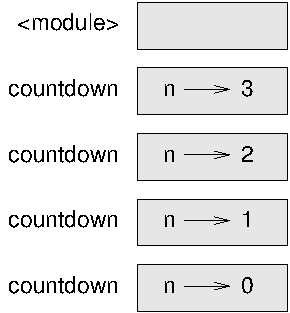
\includegraphics[scale = 0.8] {figs/stack2.pdf}}
\caption{diagrama Stack.}
\label{} fig.stack2
\end{figure}


Como de costume, o topo da pilha é a moldura para \verb "__main__".
Está vazio porque não criar quaisquer variáveis 
\Verb "__main__" ou passar quaisquer argumentos para isso.
\index{caso base}
\index{recursão caso base!}

Os quatro {\tt contagem regressiva} quadros têm valores diferentes para o
parâmetro {\tt n}. A parte inferior da pilha, em que {\tt n = 0}, é
chamado {case base \bf}. Não faz uma chamada recursiva, de modo
não há mais quadros.

\begin{} exercício
Desenhe um diagrama de pilha para \verb "print_n" chamado com
\verb "s = 'Olá'" e {\tt n = 2}.
\end{} exercício

\begin{} exercício
Escreva uma função chamada \verb "do_n" que leva uma função
objeto e um número, {\tt n}, como argumentos, e que as chamadas
a função dada {\tt n} vezes.
\end{} exercício



\section{Infinito recursão}
\index{recursão infinita}
\index{recursão! Infinito}
\index{erro de execução}
\index{erro! Runtime}
\index{} traceback

Se uma recursividade nunca chega ao caso base, ela prossegue fazendo
recursiva chama para sempre, eo programa nunca termina. Isto é
conhecido como {\bf recursão infinita}, e não é geralmente
uma boa idéia. Aqui está um programa mínimo com uma recursividade infinita:

\begin{verbatim}
def recursiva ():
    recurse ()
\end{verbatim}
%
Na maioria dos ambientes de programação, um programa com recursividade infinita
realmente não correr para sempre. Python relata um erro
mensagem quando a profundidade máxima de recursividade é alcançada:
\index{exceção! RuntimeError}
\index{} RuntimeError

\begin{verbatim}
  Arquivo "<stdin>", linha 2, em recurse
  Arquivo "<stdin>", linha 2, em recurse
  Arquivo "<stdin>", linha 2, em recurse
                  .   
                  .
                  .
  Arquivo "<stdin>", linha 2, em recurse
RuntimeError: Profundidade máxima da recursão excedido
\end{verbatim}
%
Este traceback é um pouco maior do que o que vimos no
capítulo anterior. Quando o erro ocorre, existem 1.000
{\tt recurse} quadros na pilha!


\section{entrada de teclado}
\index{entrada de teclado}

Os programas que temos escrito até agora são um pouco rude no sentido de que
eles não aceitam qualquer entrada do usuário. Eles apenas fazem a mesma coisa todos
tempo.

Python 2 fornece uma função built-in chamado \verb "raw_input", que recebe
entrada do teclado. Em Python 3, ele é chamado
  {Tt entrada \}. Quando esta função é chamada, o programa pára e
aguarda que o usuário digite alguma coisa. Quando o usuário pressiona {\sf
  Retornar} ou {\sf Enter}, o programa retoma e \verb "raw_input"
retorna o que o usuário digitou como uma string.
\index{Python 3}
\index{function \_input crua}
\index{function! \_input Crua}

\begin{verbatim}
>>> Texto = raw_input ()
O que você está esperando?
>>> Print texto
O que você está esperando?
\end{verbatim}
%
Antes de obter a entrada do usuário, que é uma boa idéia para imprimir um
solicitar informando ao usuário que a de entrada. \Verb "raw_input" pode levar um
pedir como um argumento:
\index{indicador}

\begin{verbatim}
>>> Nome = raw_input ("Qual ... é o seu nome? \N ')
O que ... é o seu nome?
Arthur, Rei dos Bretões!
>>> Print nome
Arthur, Rei dos Bretões!
\end{verbatim}
%
A seqüência \verb "\n" no final do prompt representa uma {\bf nova linha},
que é um carácter especial que faz com que uma quebra de linha.
É por isso que a entrada do usuário aparece abaixo do alerta.
\index{newline}

Se você espera que o usuário digite um número inteiro, você pode tentar converter
o valor de retorno para {\tt int}:

\begin{verbatim}
>>> Prompt = "Qual ... é a velocidade de vôo de um vazio engolir? \N '
>>> Velocidade = raw_input (prompt)
O que ... é a velocidade de vôo de uma andorinha?
17
>>> Int (velocidade)
17
\end{verbatim}
%
Mas se os tipos ao usuário algo que não seja uma seqüência de dígitos,
você receber um erro:

\begin{verbatim}
>>> Velocidade = raw_input (prompt)
O que ... é a velocidade de vôo de uma andorinha?
O que quer dizer, uma andorinha Europeia Africano ou?
>>> Int (velocidade)
ValueError: inválido literal para int ()
\end{verbatim}
%
Vamos ver como lidar com esse tipo de erro mais tarde.
\index{} ValueError
\index{exceção! V alueError}


\section{} Depuração
\label{espaços}
\index{depuração}
\index{} traceback

Os traceback Python é exibido quando ocorre um erro contém
uma grande quantidade de informações, mas pode ser esmagadora, especialmente
quando há muitos quadros na pilha. A maioria
peças úteis são geralmente:

\begin{itemize}

\item Que tipo de erro que era, e

\item onde ela ocorreu.

\end{itemize}

Os erros de sintaxe são geralmente fáceis de encontrar, mas existem alguns
pegadinhas. Erros de espaço em branco pode ser complicado porque os espaços e
guias são invisíveis e que estamos acostumados a ignorá-los.
\index{espaços}

\begin{verbatim}
>>> X = 5
>>> Y = 6
  Arquivo "<stdin>", linha 1
    y = 6
    ^
SyntaxError: sintaxe inválida
\end{verbatim}
%
Neste exemplo, o problema é que a segunda linha é recuada por
um espaço. Mas a mensagem de erro indica {\tt y}, que é
enganosa. Em geral, as mensagens de erro indicam que o problema estava
descobertos, mas o erro real pode ser mais cedo no código,
às vezes em uma linha anterior.
\index{erro! Runtime}
\index{erro de execução}

O mesmo é verdadeiro de erros de execução.  

Suponha que você está tentando
para calcular uma relação sinal-para-ruído em decibéis. A fórmula
é de R $ SNR_ {db} = 10 \log_ {10} (P_ {sinal} / P_ {ruído}) $. Em Python,
você pode escrever algo como isto:

\begin{verbatim}
matemática importação
signal_power = 9
noise_power = 10
ratio = signal_power / noise_power
decibéis = 10 * math.log10 (razão)
decibéis impressão
\end{verbatim}
%
Mas quando você executá-lo em Python 2, você recebe uma mensagem de erro.
\index{exceção! OverflowError}
\index{} OverflowError

\begin{verbatim}
Traceback (most recent call last):
  Arquivo "snr.py", linha 5, em?
    decibéis = 10 * math.log10 (razão)
OverflowError: erro gama de matemática
\end{verbatim}
%
A mensagem de erro indica que a linha 5, mas não há nada
de errado com essa linha. Para encontrar o verdadeiro erro, pode ser
útil para imprimir o valor de {relação \tt}, o que acaba por
ser 0. O problema está na linha 4, porque dividir dois números inteiros
faz divisão chão. A solução é representar a potência do sinal
e potência de ruído com valores de ponto flutuante.
\index{divisão chão}
\index{divisão! Chão}

Em geral, as mensagens de erro dizer-lhe que o problema foi descoberto, 
mas que muitas vezes não é o lugar onde ele foi causado.

Em Python 3, este exemplo não causar um erro, o operador de divisão
executa divisão em ponto flutuante, mesmo com operandos inteiros.


\section{} Glossário

\begin{description}

\item[Operador módulo:] item de um operador, indicadas com um sinal de porcentagem
({\tt \%}), que trabalha com números inteiros e retorna o resto quando um
número é dividido por um outro.
\index{operador módulo}
\index{operador! Módulo}

\item[expressão booleana:] Uma expressão cujo valor é 
{\tt true} ou {\tt false}.
\index{expressão booleana}
\index{expressão! Boolean}

\item[operador relacional:] Um dos operadores que compara
operandos: {\tt ==}, {\tt =!}, {\tt>}, {\tt <}, {\tt> =} e {\tt <=}.

\item[operador lógico:] Um dos operadores que combina boolean
expressões: {\tt e}, {\tt ou} e {\tt não}.

\item[declaração condicional:] Uma declaração de que controla o fluxo de
execução dependendo de alguma condição.
\index{instrução condicional}
\index{declaração! Condicional}

\item[condição]: A expressão booleana em uma instrução condicional
que determina qual ramo é executado.
\index{condição}

\item[Instrução composta:] item A afirmação de que consiste de um cabeçalho
e um corpo. O cabeçalho termina com dois pontos (:). O corpo é recortado
em relação ao cabeçalho.
\index{instrução composta}

\item[ramo]: Uma das seqüências alternativas de declarações em
uma instrução condicional.
\index{ramo}

\item[acorrentado condicional:] A instrução condicional com uma série
de ramos alternativos.
\index{condicional encadeada}
\index{condicional! Acorrentado}

\item[aninhados condicional:] A instrução condicional que aparece
em um dos ramos de uma outra instrução condicional.
\index{nested condicional}
\index{condicional! Aninhada}

\item[recursão:] O processo de chamar a função que é
atualmente em execução.
\index{recursão}

\item[caso base:] Um ramo condicional em um
função recursiva que não faz uma chamada recursiva.
\index{caso base}

\item[recursão infinita:] A recursividade que não tem um
caso base, ou nunca alcança-lo. Eventualmente, uma recursão infinita
causa um erro de tempo de execução.
\index{recursão infinita}

\end{description}

\section{Exercícios}

\begin{} exercício
\index{Último Teorema de Fermat}

Último Teorema de Fermat diz que não existem números inteiros
$ A $, $ b $ e $ c $ tal que

\[A ^ n + b ^ n = c ^ n \]
%
para quaisquer valores de $ n $ maior do que 2.

\begin{enumerate}

\item Escreva uma função chamada \verb "check_fermat", que leva de quatro
parâmetros --- {\tt a}, {\tt b}, {\tt c} e {\tt n} --- e
que verifica se o teorema de Fermat detém. Se
$ N $ é maior que 2 e que acaba por ser verdade que 

\[A ^ n + b ^ n = c ^ n \]
%
o programa deve imprimir, `` Nossa, Fermat estava errada!''
Caso contrário, o programa deve imprimir, `` Não, isso não funciona.''

\item Escreva uma função que solicita ao usuário para valores de entrada
para {\tt a}, {\tt b}, {\tt c} e {\tt n}, converte-os em
inteiros e usa \verb "check_fermat" para verificar se eles
violar teorema de Fermat.

\end{enumerate}

\end{} exercício


\begin{} exercício
\index{triângulo}

Se você tem três varas, você pode ou não ser capaz de organizar
los em um triângulo. Por exemplo, se um dos paus é de 12 polegadas
longo e os outros dois são uma polegada de comprimento, é claro que você vai
não ser capaz de obter as varas curtas para atender no meio. Para quaisquer
três comprimentos, não é um simples teste para ver se é possível a formação
um triângulo:

\begin{citação}
Se qualquer um dos três comprimentos é maior do que a soma das outras
  dois, então você não pode formar um triângulo. Caso contrário, você
  pode. (Se a soma dos dois comprimentos é igual ao terceiro, formam
    que é chamado de `` degenerado triângulo.'')
\end{citação}

\begin{enumerate}

\item Escreva uma função chamada \verb "is_triangle", que leva de três
  inteiros como argumentos, e que imprime ou `` Sim'' ou `` Não'', dependendo
  se você pode ou não pode formar um triângulo a partir de drives com o
  dado comprimentos.

\item Escreva uma função que solicita ao usuário a entrada de três vara
  comprimentos, converte-os em números inteiros, e usa \verb "is_triangle" para
  verificar se varas com os comprimentos indicados podem formar um triângulo.

\end{enumerate}

\end{} exercício

Os exercícios a seguir usar TurtleWorld do capítulo ~ \ref {} turtlechap:
\index{} TurtleWorld

\begin{} exercício

Leia a seguir a função e veja se você pode descobrir
o que ele faz. Em seguida, executá-lo (veja os exemplos no capítulo ~ \ref {turtlechap}).

\begin{verbatim}
def desenhar (t, comprimento, n):
    se n == 0:
        retorno
    ângulo = 50
    fd (t, comprimento * n)
    lt (t, ângulo)
    desenhar (t, comprimento, n-1)
    rt (t, ângulo 2 *)
    desenhar (t, comprimento, n-1)
    lt (t, ângulo)
    bk (t, comprimento * n)
\end{verbatim}

\end{} exercício


\begin{figure}
\centerline
{\includegraphics[scale = 0.8] {figos / koch.pdf}}
\caption{A curva de Koch.}
\label{} fig.koch
\end{figure}

\begin{} exercício
\index{curva Koch}

A curva de Koch é um fractal que é algo como
Figura ~ \ref {} fig.koch. Para desenhar uma curva de Koch, com comprimento $ x $, tudo o que você
tem a fazer é

\begin{enumerate}

\item Desenhe uma curva de Koch, com comprimento $ x / 3 $.

\item de volta esquerda 60 graus.

\item Desenhe uma curva de Koch, com comprimento $ x / 3 $.

\item Vire à direita de 120 graus.

\item Desenhe uma curva de Koch, com comprimento $ x / 3 $.

\item de volta esquerda 60 graus.

\item Desenhe uma curva de Koch, com comprimento $ x / 3 $.

\end{enumerate}

A exceção é se $ x $ é inferior a 3: nesse caso,
você pode simplesmente desenhar uma linha reta com o comprimento $ x $.

\begin{enumerate}

\item Escreva uma função chamada {\tt koch} que tem uma tartaruga e
um comprimento como parâmetros, e que usa a tartaruga para desenhar uma Koch
curva com o comprimento dado.

\item Escreva uma função chamada {\tt} floco de neve que atrai três
Curvas de Koch para fazer o contorno de um floco de neve.

Solução: \url{http://thinkpython.com/code/koch.py}.

\item A curva de Koch pode ser generalizado de várias maneiras. Ver
\url{} http://en.wikipedia.org/wiki/Koch_snowflake para exemplos e
implementar o seu favorito.

\end{enumerate}
\end{} exercício


\chapter{funções frutíferas}
\label{} fruitchap

\section{Valores de retorno}
\index{valor de retorno}

Algumas das funções internas que usamos, como a matemática
funções, produzir resultados. Chamando a função gera um
valor, que geralmente atribuímos a uma variável ou usar como parte de um
expressão.

\begin{verbatim}
e = math.exp (1.0)
height = raio * math.sin (radianos)
\end{verbatim}
%
Todas as funções que temos escrito até agora são nulos; eles imprimem
algo ou mover tartarugas ao redor, mas o seu valor de retorno é {\tt
Nenhum}.

Neste capítulo, estamos (finalmente) vai escrever funções produtivas.
O primeiro exemplo é a área de {tt \}, o qual retorna à área de um círculo
com o raio dada:

\begin{verbatim}
área def (raio):
    temp = math.pi * raio ** 2
    temp
\end{verbatim}
%
Vimos o {return \tt} declaração antes, mas em uma frutífera
funcionar a {return \tt} declaração inclui
uma expressão. Essa afirmação significa: `` Retorne imediatamente a partir de
esta função e usar a seguinte expressão como um valor de retorno.''
A expressão pode ser arbitrariamente complicada, de modo que pudéssemos
ter escrito esta função de forma mais concisa:
\index{instrução de retorno}
\index{declaração! Retorno}

\begin{verbatim}
área def (raio):
    voltar math.pi * raio ** 2
\end{verbatim}
%
Por outro lado, {\bf variáveis ​​temporárias} como {\tt temperatura} muitas vezes fazem
depuração mais fácil.
\index{variável temporária}
\index{variável! Temporário}

Às vezes é útil ter múltiplos comandos return, um em cada
ramo de uma condicional:

\begin{verbatim}
def absolute_value (x):
    if x <0:
        voltar-x
    else:
        voltar x
\end{verbatim}
%
Uma vez que estes {return \tt} declarações estão em uma condição alternativa,
apenas um será executado.

Assim que uma instrução de retorno é executado, a função
termina sem executar quaisquer declarações subseqüentes.
O código que aparece depois de um {return \tt} declaração, ou qualquer outro local
o fluxo de execução nunca pode alcançar, é chamado {\bf código morto}.
\index{código morto}

Em uma função frutífera, é uma boa idéia para garantir
que todos os caminhos possíveis através do programa atinge um
{Return \tt} comunicado. Por exemplo:

\begin{verbatim}
def absolute_value (x):
    if x <0:
        voltar-x
    se x> 0:
        voltar x
\end{verbatim}
%
Esta função está incorreta porque se {\tt x} passa a ser 0,
nem condição é verdadeira, ea função terminará sem encontrar um
{Return \tt} comunicado. Se o fluxo de execução chega ao fim
de uma função, o valor de retorno é {\tt Nenhum}, que não é
o valor absoluto de 0.
\index{Nenhum valor especial}
\index{valor especial! Nenhum}

\begin{verbatim}
>>> Absolute_value print (0)
Nenhum
\end{verbatim}
%
By the way, Python fornece uma função built-in chamado 
{\tt abs} que calcula valores absolutos.
\index{função abs}
\index{function! Abs}

\begin{} exercício
\index{comparar função}
\index{function! Comparar}

Escreva uma função {\tt comparar}
que os retornos {\tt 1} se {\tt x> y},
{\tt 0} se {\tt x == y} e {\tt -1} if {\tt x <y}.
\end{} exercício


\section{desenvolvimento incremental}
\label{} incremental.development
\index{plano de desenvolvimento! Incrementais}

Como você escrever funções maiores, você pode encontrar-se
gastando mais tempo de depuração.

Para lidar com programas cada vez mais complexos,
você pode querer experimentar um processo chamado
{\bf desenvolvimento incremental}. A meta do desenvolvimento incremental
é evitar longas sessões de depuração ao adicionar e testar somente
uma pequena quantidade de código de cada vez.
\index{teste! Desenvolvimento incremental}
\index{teorema de Pitágoras}

Como exemplo, suponha que você queira saber a distância entre dois
pontos, dada pelas coordenadas $ (x_1, y_1) $ e $ (x_2, y_2) $.
Pelo teorema de Pitágoras, a distância é:

\begin{displaymath}
\Mathrm {distância} = \sqrt {(x_2 - x_1) ^ 2 + (y_2 - y_1) ^ 2}
\end{displaymath}
%
O primeiro passo é considerar o que uma função distância {\tt} deve
parecer em Python. Em outras palavras, quais são as entradas (parâmetros)
e qual é a saída (valor de retorno)?

Neste caso, as entradas são dois pontos, que você pode representar
usando quatro números. O valor de retorno é a distância, o que é
um valor de ponto flutuante.

Já é possível escrever um esboço da função:

\begin{verbatim}
distância def (x1, y1, x2, y2):
    retornar 0,0
\end{verbatim}
%
Obviamente, esta versão não calcula distâncias, mas sempre retorna
zero. Mas é sintaticamente correto, e ele é executado, o que significa que
você pode testá-lo antes de torná-lo mais complicado.

Para testar a nova função, chamá-lo com argumentos de exemplo:

\begin{verbatim}
>>> Distância (1, 2, 4, 6)
0,0
\end{verbatim}
%
Escolhi estes valores, de modo que a distância horizontal é 3 e o
distância vertical é 4, dessa forma, o resultado é de 5
(A hipotenusa de um triângulo 3-4-5). Ao testar uma função, é
útil para saber a resposta certa.
\index{teste! Sabendo a resposta}

Neste ponto, nós confirmamos que a função está sintaticamente
corrigir, e podemos começar a adicionar código para o corpo.
Um próximo passo razoável é encontrar as diferenças
$ X_2 - x_1 $ e $ y_2 - y_1 $. A próxima versão armazena esses valores em
variáveis ​​temporárias e as imprime.

\begin{verbatim}
distância def (x1, y1, x2, y2):
    dx = x2 - x1
    dy = y2 - y1
    print 'dx é', dx
    print 'dy é', dy
    retornar 0,0
\end{verbatim}
%
Se a função está funcionando, ele deve exibir \verb "'dx é 3'" e {\tt
'Dy é 4'}. Se assim for, sabemos que a função é obter o direito
argumentos e realizar o primeiro cálculo corretamente. Se não,
há apenas algumas linhas para verificar.

Em seguida, calcular a soma dos quadrados dos {\tt dx} e {\tt dy}:

\begin{verbatim}
distância def (x1, y1, x2, y2):
    dx = x2 - x1
    dy = y2 - y1
    Dsquared = dx ** 2 + dy ** 2
    print 'dsquared é:', Dsquared
    retornar 0,0
\end{verbatim}
%
Mais uma vez, você deve executar o programa neste estágio e checar a saída
(Que deve ser de 25).
Finalmente, você pode usar {\tt math.sqrt} para calcular e retornar o resultado:
\index{sqrt}
\index{function! Sqrt}

\begin{verbatim}
distância def (x1, y1, x2, y2):
    dx = x2 - x1
    dy = y2 - y1
    Dsquared = dx ** 2 + dy ** 2
    result = math.sqrt (dsquared)
    resultado de retorno
\end{verbatim}
%
Se isso funcionar corretamente, você está feito. Caso contrário, você pode
deseja imprimir o valor de {resultado \tt} antes do retorno
comunicado.

A versão final da função não exibe nada quando se
executado, que só retorna um valor. O {\tt impressão} declarações que escrevemos
são úteis para a depuração, mas quando você começa o trabalho função,
deve removê-los. Código como este é chamado {\bf andaimes}
vez que é útil para o programa, mas não faz parte da
produto final.
\index{} andaimes

Quando você começa, você deve adicionar apenas uma ou duas linhas de código de cada
tempo. Como você ganhar mais experiência, você pode encontrar-se a escrever
e depuração de pedaços maiores. De qualquer maneira, desenvolvimento incremental
você pode salvar um monte de tempo de depuração.

Os aspectos-chave do processo são:

\begin{enumerate}

\item Comece com um programa de trabalho e fazer pequenas mudanças incrementais. 
A qualquer momento, se houver um erro, você deve ter uma boa idéia
onde está.

\item Use variáveis ​​temporárias para manter valores intermediários para que você possa
exibir e verificá-los.

\item Uma vez que o programa está funcionando, você pode querer remover alguns dos
o andaime ou consolidar múltiplos comandos no composto
expressões, mas somente se ele não tornar o programa difícil
ler.

\end{enumerate}

\begin{} exercício
\index{hipotenusa}

Use desenvolvimento incremental para escrever uma função
chamado {\tt hipotenusa} que retorna o comprimento da hipotenusa de um
triângulo retângulo dado os comprimentos das duas pernas como argumentos.
Registre cada fase do processo de desenvolvimento que você vá.
\end{} exercício


\section{Composição}
\index{composição}
\index{composição função}

Como você deve esperar por agora, você pode chamar uma função de
dentro de um outro. Esta habilidade é chamada de composição {\bf}.

Como exemplo, vamos escrever uma função que recebe dois pontos,
o centro do círculo e um ponto sobre o perímetro, e calcula
a área do círculo.

Suponha que o ponto central é armazenado nas variáveis ​​{\tt xc} e
{\tt yc}, eo ponto do perímetro está na {\tt xp} e {\tt yp}. O
primeiro passo é o de encontrar o raio do círculo, que é a distância
entre os dois pontos. Nós apenas escreveu uma função, {\tt
distância}, que faz isso:

\begin{verbatim}
raio = distância (xc, yc, xp, yp)
\end{verbatim}
%
O próximo passo é para que a área de um círculo cujo raio;
nós apenas escreveu que, também:

\begin{verbatim}
result = área (raio)
\end{verbatim}
%
Encapsulando estes passos em uma função, temos:
\index{} encapsulamento

\begin{verbatim}
circle_area def (xc, yc, xp, yp):
    raio = distância (xc, yc, xp, yp)
    result = área (raio)
    resultado de retorno
\end{verbatim}
%
As variáveis ​​temporárias raio {\tt} e {resultado \tt} são úteis para
desenvolvimento e depuração, mas uma vez que o programa está funcionando, podemos
torná-lo mais conciso através da composição das chamadas de função:

\begin{verbatim}
circle_area def (xc, yc, xp, yp):
    área de retorno (distância (xc, yc, xp, yp))
\end{verbatim}
%

\section{} funções booleanas
\label{boolean}

Funções podem retornar valores booleanos, o que muitas vezes é conveniente para esconder
testes complicados dentro de funções. \index{função booleana}
Por exemplo:

\begin{verbatim}
def is_divisible (x, y):
    se xy == 0:
        retornar True
    else:
        retornará False
\end{verbatim}
%
É comum dar funções booleanas nomes que soam como sim / não
perguntas; \verb "is_divisible" retorna {\tt true} ou {\tt false}
para indicar se {\tt x} é divisível por {\tt y}.

Aqui está um exemplo:

\begin{verbatim}
>>> Is_divisible (6, 4)
Falso
>>> Is_divisible (6, 3)
Verdadeiro
\end{verbatim}
%
O resultado da {\tt ==} operador é um boolean, então podemos escrever a
funcionar de forma mais concisa, retornando-lo diretamente:

\begin{verbatim}
def is_divisible (x, y):
    voltar xy == 0
\end{verbatim}
%
Funções booleanas são muitas vezes utilizados em comandos condicionais:
\index{instrução condicional}
\index{declaração! Condicional}

\begin{verbatim}
is_divisible se (x, y):
    imprimir 'x é divisível por y'
\end{verbatim}
%
Pode ser tentador para escrever algo como:

\begin{verbatim}
se is_divisible (x, y) == true:
    imprimir 'x é divisível por y'
\end{verbatim}
%
Mas a comparação adicional é desnecessária.

\begin{} exercício

Escreva uma função \verb "is_between (x, y, z)" que
retornos {\tt true} if $ x \le y \le z $ ou {\tt false} contrário.

\end{} exercício


\section{Mais recursão}
\label{} more.recursion
\index{recursão}
\index{Turing linguagem completa}
\index{língua! Turing completo}
\index{Turing, Alan}
\index{Turing Tese}

Nós só ter coberto um pequeno subconjunto de Python, mas você pode
estar interessado em saber que este é um subconjunto {\em completar}
linguagem de programação, o que significa que qualquer coisa que pode ser
calculado pode ser expresso nessa língua. Qualquer programa já escrito
poderia ser reescrito usando apenas os recursos de linguagem que você aprendeu
até agora (na verdade, você precisaria de alguns comandos para controlar dispositivos
como o teclado, mouse, discos, etc, mas isso é tudo).

Provando que a afirmação é um exercício trivial primeiro realizado por Alan
Turing, um dos primeiros cientistas da computação (alguns diriam que ele
foi um matemático, mas um monte de cientistas da computação começaram como
matemáticos). Assim, ela é conhecida como a Tese de Turing.
Para uma discussão mais completa (e preciso) da Tese de Turing,
Eu recomendo o livro de Michael Sipser {\em Introdução ao
Teoria da Computação}.

Para se ter uma idéia do que você pode fazer com as ferramentas que você aprendeu
até agora, vamos avaliar algumas matemática definida recursivamente
funções. Uma definição recursiva é semelhante a uma circular
definição, no sentido de que a definição de uma referência a
a coisa a ser definida. Uma verdadeira definição circular não é muito
útil:

\begin{description}

\item[vorpal:] Um adjetivo usado para descrever algo que é vorpal.
\index{} vorpal
\index{definição circular}
\index{definição! Circular}

\end{description}

Se você viu que a definição no dicionário, você pode ser aborrecido. Em
Por outro lado, se você olhou a definição do fatorial
função, denotada com o símbolo $!$, que você pode obter algo como
este:
%
\begin{eqnarray *}
&& 0! = 1 \\
&& N! = N (n-1)!
\end{eqnarray *}
%
Esta definição diz que o fatorial de 0 é 1, eo fatorial
de qualquer outro valor, $ n $, é de US $ n $ multiplicado pelo fatorial de $n-1$.

Portanto, $3!$ É 3 vezes $2!$, Que é 2 vezes $1!$, Que é 1 vezes
$0!$. Juntando tudo, $3!$ Equivale a 3 vezes 2 vezes 1 vezes 1,
o qual é 6.
\index{função fatorial}
\index{function! Fatorial}
\index{definição recursiva}

Se você pode escrever uma definição recursiva de alguma coisa, você pode geralmente
escrever um programa Python para avaliá-lo. O primeiro passo é decidir
o que os parâmetros devem ser. Neste caso, deve ser claro
que {\tt fatorial} leva um inteiro:

\begin{verbatim}
def fatorial (n):
\end{verbatim}
%
Se o argumento passa a ser 0, tudo o que temos a fazer é retorno 1:

\begin{verbatim}
def fatorial (n):
    se n == 0:
        retornar 1
\end{verbatim}
%
Caso contrário, e isto é a parte interessante, temos que fazer uma
chamada recursiva para encontrar o fatorial de n-1 $ $ e, em seguida, multiplicá-lo por
$ N $:

\begin{verbatim}
def fatorial (n):
    se n == 0:
        retornar 1
    else:
        recursivo = fatorial (n-1)
        resultado = n * recurse
        resultado de retorno
\end{verbatim}
%
O fluxo de execução para este programa é semelhante ao fluxo de {\tt
contagem regressiva} na Seção ~ \ref {recursão}. Se chamarmos fatorial {\tt}
com o valor 3:

Desde 3 não é 0, tomamos o segundo ramo e calculamos o fatorial
de {\tt n-1} ...

\begin{quote}
Desde 2 não é 0, tomamos o segundo ramo e calculamos o fatorial de
{\tt n-1} ...


  \begin{quote}
  Desde 1 não é 0, tomamos o segundo ramo e calculamos o fatorial
  de {\tt n-1} ...


    \begin{quote}
    Desde 0 {\em} é 0, tomamos o primeiro ramo e retornar 1
    sem fazer mais chamadas recursivas.
    \end{quote}


  O valor de retorno (1) é multiplicado por n $ $, que é 1, e o
  resultado é retornado.
  \end{quote}


O valor de retorno (1) é multiplicado por n $ $, que é a 2, e o
resultado é retornado.
\end{quote}


O valor de retorno (2) é multiplicado por n $ $, que é 3, e o resultado, 6,
torna-se o valor de retorno da chamada de função que iniciou a todo
processo.
\index{diagrama de pilha}

Figura ~ \ref {} fig.stack3 mostra o que o diagrama de pilha para
essa seqüência de chamadas de função.

\begin{figure}
\centerline
{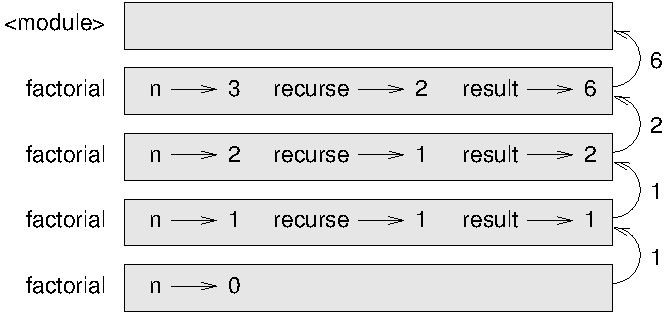
\includegraphics[scale = 0.8] {figs/stack3.pdf}}
\caption{diagrama Stack.}
\label{} fig.stack3
\end{figure}

Os valores de retorno são mostrados sendo passados ​​para trás até a pilha. Em cada
quadro, o valor de retorno é o valor do resultado {\tt}, que é o
produto de {\tt n} e {\tt recurse}.
\index{função frame}
\index{frame}

No último quadro, o local de
variáveis ​​{\tt recurse} e {resultado \tt} não existem, porque
o ramo que os cria não executa.


\section{Leap of faith}
\index{recursão}
\index{salto de fé}

Seguindo o fluxo de execução é uma maneira de ler programas, mas
ele pode rapidamente tornar-se labiríntico. Uma
alternativa é o que eu chamo de `` salto de fé.'' Quando você chegar a uma
chamada de função, em vez de seguir o fluxo de execução, você {\em
assumir} que a função funciona corretamente e retorna o direito
resultado.

Na verdade, você já está praticando esse salto de fé quando você usa
built-in funções. Quando você chamar {\tt math.cos} ou {\tt math.exp},
você não examinar os corpos de essas funções. Você só
supor que eles funcionam porque as pessoas que escreveram o built-in
funções eram bons programadores.

O mesmo é verdadeiro quando você chamar um dos suas próprias funções. Para
exemplo, na Seção ~ \ref {boolean}, escrevemos uma função chamada 
\verb"is_divisible" que determina se um número é divisível por
outro. Uma vez que nós nos convencemos que esta função é
correto --- através da análise do código e os testes --- podemos usar a função
sem olhar para o corpo novamente.
\index{teste! Salto de fé}

O mesmo é verdadeiro para programas recursivos. Quando você chegar ao recursiva
chamar, em vez de seguir o fluxo de execução, você deve assumir
que as obras de chamadas recursivas (produz o resultado correto) e depois pedir
mesmo, `` Assumindo que eu possa encontrar o fatorial de n-1 $ $, eu posso
calcular o fatorial de n $ $?'' Neste caso, é claro que você
pode, multiplicando por $ n $.

Claro, é um pouco estranho supor que a função funciona
corretamente quando você não terminei de escrevê-lo, mas é por isso que
chama-se um salto de fé!


\section{Mais um exemplo}
\label{} one.more.example

\index{função Fibonacci}
\index{function! Fibonacci}
Depois {\tt fatorial}, o exemplo mais comum de uma forma recursiva
função matemática definida é {\tt Fibonacci}, que tem a
seguinte definição (ver
  \url{http://en.wikipedia.org/wiki/Fibonacci_number}):
%
\begin{eqnarray *}
&& \Mathrm {} Fibonacci (0) = 0 \\
&& \Mathrm {} Fibonacci (1) = 1 \\
&& \Mathrm {} Fibonacci (n) = \mathrm {} Fibonacci (n-1) + \mathrm {} Fibonacci (n-2)
\end{eqnarray *}
%
Traduzido em Python, ele se parece com isso:

\begin{verbatim}
Fibonacci def (n):
    se n == 0:
        retornar 0
    elif n == 1:
        retornar 1
    else:
        Fibonacci retorno (n-1) + Fibonacci (n-2)
\end{verbatim}
%
Se você tentar seguir o fluxo de execução aqui, mesmo para razoavelmente
pequenos valores de $ n $, sua cabeça explode. Mas de acordo com o
salto de fé, se você assume que as duas chamadas recursivas
funcionar corretamente, então é claro que você obtenha
o resultado certo, adicionando-os juntos.
\index{fluxo de execução}


\section{Verificando tipos}
\label{guardião}

O que acontece se nós chamamos {\tt fatorial} e dar-lhe 1.5 como argumento?
\index{verificação de tipo}
\{Verificação de erros} índice
\index{função fatorial}
\index{} RuntimeError

\begin{verbatim}
>>> Fatorial (1.5)
RuntimeError: Profundidade máxima da recursão excedido
\end{verbatim}
%
Parece que uma recursão infinita. Mas como pode ser isso? Há um
caso base --- quando {\tt n == 0}. Mas se {\tt n} não é um número inteiro,
podemos {\em falta} o caso base e recursivo para sempre.
\index{recursão infinita}
\index{recursão! Infinito}

Na primeira chamada recursiva, o valor de {\tt n} é 0.5.
No próximo, é -0,5. A partir daí, torna-se menor
(Mais negativo), mas ele nunca vai ser 0.

Nós temos duas escolhas. Podemos tentar generalizar o fatorial {\tt}
função para trabalhar com números de ponto flutuante, ou podemos fazer {\tt
  fatorial} verificar o tipo de argumento. A primeira opção é
chamado a função gama e é uma
pouco além do escopo deste livro. Então vamos para o segundo.
\index{função gama}

Podemos usar a função built-in {\tt isinstance} para verificar o tipo de
do argumento. Enquanto estamos no assunto, também podemos garantir que o
argumento é positivo:
\index{function isinstance}
\index{function! Isinstance}

\begin{verbatim}
def fatorial (n):
    se não isinstance (n, int):
        imprimir "Fatorial somente é definido para inteiros.
        Nenhum retorno
    elif n <0:
        print 'fatorial não está definido para inteiros negativos.
        Nenhum retorno
    elif n == 0:
        retornar 1
    else:
        retornar n * fatorial (n-1)
\end{verbatim}
%
O primeiro caso trata de base não-inteiros, o
segundo pega inteiros negativos. Em ambos os casos, o programa imprime
uma mensagem de erro e retorna {\tt none} para indicar que algo
deu errado:

\begin{verbatim}
>>> Fatorial ('fred')
Fatorial somente é definido para inteiros.
Nenhum
>>> Fatorial (-2)
Fatorial não está definido para inteiros negativos.
Nenhum
\end{verbatim}
% 
Se passarmos pelas duas checagens, então sabemos que $ n $ é positivo ou
zero, para que possamos provar que a recursão termina.
\index{padrão guardião}
\index{padrão! Guardião}

Este programa demonstra um padrão muitas vezes chamado de {\bf guardião}.
As duas primeiras condicionais atuam como guardiãs, protegendo o código que
seguida de valores que possam causar um erro. Os guardiões torná-lo
possível comprovar a correção do código.

Na Seção ~ \ref{raise} veremos uma alternativa mais flexível para impressão
uma mensagem de erro: levantar uma exceção.


\section{Depuração}
\label{factdebug}

Quebrando um grande programa em funções menores cria naturais
checkpoints para depuração. \index{depuração}
Se uma função não está funcionando, há
três possibilidades a considerar:

\begin{itemize}

\item Há algo de errado com os argumentos da função
está ficando, uma pré-condição é violada.

\item Há algo de errado com a função; uma pós-condição
é violada.

\item Há algo de errado com o valor de retorno ou a
forma como ele está sendo usado.

\end{itemize}

Para descartar a primeira hipótese, você pode adicionar um {\tt print} declaração
no início da função e exibir os valores da
parâmetros (e talvez os seus tipos). Ou você pode escrever código
que verifica os pré-requisitos explicitamente.
\index{condição}
\index{pós-condição}

Se os parâmetros de boa aparência, adicionar uma {\tt print} declaração antes de cada
{Return \tt} declaração que exibe o valor de retorno. Se
possível, verificar o resultado com a mão. Considere chamando o
função com valores que tornam mais fácil para verificar o resultado
(Como na Seção ~ \ref {incremental.development}).

Se a função parece estar funcionando, olhe para a chamada de função
para garantir que o valor de retorno está sendo usado corretamente (ou usado
em tudo!).
\index{fluxo de execução}

Adicionando instruções de impressão no início e no final de uma função
pode ajudar a tornar o fluxo de execução mais visível.
Por exemplo, aqui está uma versão do {\tt fatorial} com
instruções de impressão:

\begin{verbatim}
def fatorial (n):
    espaço = '' * (4 * n)
    espaço de impressão, 'fatorial', n
    se n == 0:
        espaço de impressão ', retornando 1'
        retornar 1
    else:
        recursivo = fatorial (n-1)
        resultado = n * recurse
        espaço de impressão, 'retorno', resultado
        resultado de retorno
\end{verbatim}
%
{Espaço \tt} é uma seqüência de caracteres de espaço que controla a
recuo da saída. Aqui está o resultado de {\tt fatorial (5)}:

\begin{verbatim}
                     fatorial 5
                 fatorial 4
             fatorial 3
         fatorial 2
     fatorial 1
 fatorial 0
 retornando 1
     retornando 1
         voltando 2
             retornando 6
                 retornando 24
                     retornando 120
\end{verbatim}
%
Se você está confuso sobre o fluxo de execução, esse tipo de
saída pode ser útil. Leva algum tempo para se desenvolver eficaz
andaime, mas um pouco de andaimes pode salvar um monte de depuração.


\section{} Glossário

\begin{description}

\item[variável temporária:] Uma variável usada para armazenar um valor intermediário em
um cálculo complexo.
\index{variável temporária}
\index{variável! Temporário}

\item[code mortos:] Parte de um programa que não pode nunca ser executado, porque muitas vezes
ele aparece depois de um {return \tt} comunicado.
\index{código morto}

\item[{\tt Nenhum}:] Um valor especial retornado por funções que
não têm nenhuma instrução de retorno ou uma instrução de retorno sem um argumento.
\index{Nenhum valor especial}
\index{valor especial! Nenhum}

\item[desenvolvimento incremental:] Um plano de desenvolvimento programa destinado a
evita a depuração ao adicionar e testar somente
uma pequena quantidade de código de cada vez.
\index{desenvolvimento incremental}

\item[andaime:] O código que é usado durante o desenvolvimento do programa, mas é
não faz parte da versão final.
\index{} andaimes

\item[guardião]: Um padrão de programação que usa uma condicional
declaração para verificar e lidar com circunstâncias que
pode causar um erro.
\index{padrão guardião}
\index{padrão! Guardião}

\end{description}


\section{Exercícios}

\begin{} exercício

Desenhe um diagrama de pilha para o programa seguinte. O que faz o programa imprimir?
Solução: \url{http://thinkpython.com/code/stack_diagram.py}.
\index{diagrama de pilha}

\begin{verbatim}
def b (z):
    prod = a (z, z)
    print z, prod
    voltar prod

def A (x, y):
    x = x + 1
    retornar x * y

def c (x, y, z):
    Total = x + y + z
    quadrados = b (total) ** 2
    voltar quadrado

x = 1
y = x + 1
impressão c (x, y 3, x + y)
\end{verbatim}

\end{} exercício


\begin{} exercício
\label{} ackermann

A função de Ackermann, $ A (m, n) $, é definida:

\begin{eqnarray *}
A (m, n) = \begin {casos} 
              n +1 & \mbox {if} m = 0 \\
        A (m-1, 1) & \mbox {if} m> 0 \mbox {e} n = 0 \\
A (m-1, A (m, n-1)) & \mbox {if} m> 0 \mbox {e} n> 0.
\end{casos} 
\end{eqnarray *}
%
Veja \url{http://en.wikipedia.org/wiki/Ackermann_function}.
Escreva uma função chamada {\tt ack} que avalia a função de Ackermann.
Use sua função para avaliar {\tt ack (3, 4)}, o qual deve ser de 125.
O que acontece para valores maiores de {\tt m} e {\tt n}?
Solução: \url{http://thinkpython.com/code/ackermann.py}.
\index{função de Ackermann}
\index{function! Ack}

\end{} exercício


\begin{} exercício
\label{palíndromo}

Um palíndromo é uma palavra que está escrita a mesma para trás e
para a frente, como `` meio-dia'' e `` redivider''. Recursivamente, uma palavra
é um palíndromo se as primeiras e últimas letras são as mesmas
e meio é um palíndromo.
\index{palíndromo}

A seguir, são funções que recebem um argumento de cadeia e
retornar os primeiros, últimos e meia letras:

\begin{verbatim}
def primeiro (palavra):
    palavra voltar [0]

def última (palavra):
    palavra retorno [-1]

meio def (palavra):
    voltar palavra [1: -1]
\end{verbatim}
%
Vamos ver como eles trabalham no capítulo ~ \ref {} cordas.

\begin{enumerate}

\item Digite estas funções em um arquivo chamado {\tt palindrome.py}
e testá-los para fora. O que acontece se você chamar {\tt meio} com
uma string com duas letras? Uma carta? E o vazio
string, que é escrito \verb "''" e não contém cartas?

\item Escreva uma função chamada \verb "is_palindrome" que leva
um argumento de cadeia e retorna {\tt true} se é um palíndromo
e {\tt false} contrário. Lembre-se que você pode usar o
função built-in {\tt len} para verificar o comprimento de uma corda.

\end{enumerate}

Solução: \url{http://thinkpython.com/code/palindrome_soln.py}.

\end{} exercício

\begin{} exercício

Um número, $ a $, é uma potência de $ b $ se ele é divisível por $ b $
e $ a / b $ é uma potência de $ b $. Escreva uma função chamada
\Verb "is_power" que usa parâmetros {\tt um} e {\tt b}
e retorna {\tt true} se {\tt a} é uma potência de {\tt b}.
Nota: você terá que pensar sobre o caso base.

\end{} exercício


\begin{} exercício
\index{máximo divisor comum (GCD)}
\index{GCD (maior divisor comum)}

O máximo divisor comum (GCD) de $ a $ e $ b $ é o maior número
que separa os dois sem resto.  

Uma maneira de encontrar o MDC de dois números é o algoritmo de Euclides,
que se baseia na observação de que, se $ r $ é o restante
quando $ a $ é dividido por $ b $, então $ mdc (a, b) = mdc (b, r) $.
Como um caso base, podemos utilizar $ mdc (a, 0) = a $.
\index{algoritmo de Euclides}
\index{algoritmo! Euclides}

Escreva uma função chamada
\Verb "mdc" que usa parâmetros {\tt um} e {\tt b}
e retorna o seu máximo divisor comum. Se você precisar
ajuda, consulte \url{http://en.wikipedia.org/wiki/Euclidean_algorithm}.

Crédito: Este exercício é baseado em um exemplo de Abelson e
{Estrutura \em e Interpretação de Programas de Computador} de Sussman.

\end{} exercício


\chapter{iteração}

\section{atribuição múltipla}
\index{atribuição}
\index{declaração! Atribuição}
\index{atribuição múltipla}

Como você deve ter descoberto, é legal
fazer mais de uma tarefa para a mesma variável. A
nova atribuição faz uma variável existente referir-se a uma nova
valor (e parar de se referir ao valor de idade).

\begin{verbatim}
bruce = 5
imprimir bruce,
bruce = 7
imprimir bruce
\end{verbatim}
%
A saída deste programa é {\tt 5 7}, porque pela primeira vez
{\tt bruce} é impresso, o seu valor é de 5, e da segunda vez, a sua
valor é 7. O
vírgula no final dos primeiros suprime {\tt print} Declaração
a nova linha, que é por isso que ambas as saídas
aparecem na mesma linha.
\index{newline}

Figura ~ \ref {} fig.assign2 mostra o que {\bf atribuição múltipla} olhares
como em um diagrama de estado. \index{diagrama de estado} \index {estado diagrama!}

Com atribuição múltipla é especialmente importante para distinguir
entre uma operação de atribuição e uma declaração da igualdade. Porque
Python usa o sinal de igual ({\tt =}) para atribuição, é tentador
interpretar uma declaração como {\tt a = b} como uma afirmação da igualdade. Ele
não é!
\index{igualdade e atribuição}

Em primeiro lugar, a igualdade é uma relação simétrica e atribuição não é. Para
exemplo, em matemática, se a = 7 $ $, então $ 7 = a $. Mas em Python, o
declaração {\tt a = 7} é legal e {\tt 7 = a} não é.

Além disso, em matemática, uma expressão de igualdade é verdadeira ou
falsa, pois todos os tempos. Se a = $ b $ agora, então $ a $ será sempre igual a $ b $.
Em Python, um comando de atribuição pode tornar duas variáveis ​​iguais, mas
eles não tem que ficar assim:

\begin{verbatim}
a = 5
b = a # A e B agora são iguais
a = 3 # A e B não são iguais
\end{verbatim}
%
A terceira linha muda o valor de {\tt a}, mas não altera o
valor de {\tt b}, para que eles não são iguais. 

Apesar de atribuição múltipla é frequentemente útil, você deve usá-lo
com cautela. Se os valores das variáveis ​​mudam com freqüência, ele pode
tornar o código difícil de ler e depurar.

\begin{figure}
\centerline
{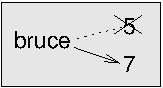
\includegraphics[scale = 0.8] {figs/assign2.pdf}}
\caption{Diagrama de Estado.}
\label{} fig.assign2
\end{figure}



\section{Atualizando variáveis}
\label{update}

\index{update}
\index{variável! Atualização}

Uma das formas mais comuns de atribuição múltipla é uma {\bf update},
onde o novo valor da variável depende da idade.

\begin{verbatim}
x = x +1
\end{verbatim}
%
Isso significa `` obter o valor atual de {\tt x}, adicione um, e, em seguida,
atualização {\tt x} com o novo valor.''

Se você tentar atualizar uma variável que não existe, você recebe um
erro, porque Python avalia o lado direito antes de ele atribui
um valor de {\tt x}:

\begin{verbatim}
>>> X = x +1
NameError: nome 'x' não está definido
\end{verbatim}
%
Antes que você pode atualizar uma variável, você tem que {\bf initialize}
que, geralmente com uma atribuição simples:
\index{inicialização (antes de atualização)}

\begin{verbatim}
>>> X = 0
>>> X = x +1
\end{verbatim}
%
Atualizando uma variável, adicionando 1 é chamado um incremento {\bf};
subtraindo 1 é chamado de decremento {\bf}.
\index{incremento}
\index{} decremento




\section{A {\tt enquanto} declaração}
\index{declaração! Enquanto}
\index{while}
\index{laço! Enquanto}
\index{iteração}

Computadores são muitas vezes utilizados para automatizar tarefas repetitivas. Repetindo
tarefas idênticas ou similares sem cometer erros é algo que
computadores fazem bem e as pessoas fazem mal.

Vimos dois programas, {\tt contagem regressiva} e \verb "print_n", que
usar recursão para executar a repetição, que também é chamado {\bf
iteração}. Porque iteração é tão comum, Python fornece vários
recursos de linguagem para torná-lo mais fácil. Um deles é o {\tt for} declaração
vimos na Seção ~ \ref {} repetição. Voltaremos a isso mais tarde.

Outro é o {\tt enquanto} comunicado. Aqui está uma versão do {\tt
contagem regressiva} que usa uma {\tt enquanto} declaração:

\begin{verbatim}
contagem regressiva def (n):
    enquanto n> 0:
        print n
        n = n-1
    imprimir 'Fogo!'
\end{verbatim}
%
Você quase pode ler o {\tt enquanto} declaração como se fosse Inglês.
Isso significa, `` Enquanto {\tt n} é maior que 0,
exibir o valor de {\tt n} e, em seguida, reduzir o valor de
{\tt n} em 1. Quando você chegar a 0, exibir a palavra {\tt Fogo!}''
\index{fluxo de execução}

Mais formalmente, aqui é o fluxo de execução para um {\tt enquanto} declaração:

\begin{enumerate}

\item Avaliar a condição, resultando {\tt true} ou {\tt false}.

\item Se a condição for falsa, sair do {\tt enquanto} declaração
e continuar a execução na próxima declaração.

\item Se a condição for verdadeira, execute o
corpo e, em seguida, volte para o passo 1.

\end{enumerate}

Este tipo de fluxo é chamado um circuito {\bf} porque a terceira etapa
loops de volta ao redor para o topo.  
\index{condição}
\index{laço}
\index{corpo}

O corpo do circuito deve alterar o valor de uma ou mais variáveis
de modo que, eventualmente, a condição se torna falsa eo loop
termina. Caso contrário, o ciclo se repetirá para sempre, que é chamado
uma {\bf Infinite Loop}. Uma fonte inesgotável de diversão para computador
os cientistas é a observação de que as instruções no shampoo,
`` Ensaboe, enxague, repita'', é um loop infinito.
\index{loop infinito}
\index{laço! Infinito}

No caso de {\tt contagem regressiva}, podemos provar que o loop
termina, pois sabemos que o valor de {\tt n} é finito, e nós
pode ver que o valor de {\tt n} fica menor a cada vez através do
loop, então, eventualmente, temos que chegar a 0. Em outra
casos, não é tão fácil dizer:

\begin{verbatim}
sequência def (n):
    enquanto n = 1:
        print n,
        se n2 == 0: # n é par
            n = n / 2
        else: # n é ímpar
            n = n * 3 +1
\end{verbatim}
%
A condição para este loop é {\tt n! = 1}, então o loop continuará
até {\tt n} é {\tt 1}, o que torna a condição falsa.

Cada vez através do loop, o programa gera o valor de {\tt n}
e verifica se é par ou ímpar. Se for mesmo, {\tt n} é
dividido por dois. Se for impar, o valor de {\tt n} é substituído com
{\tt n * 3 +1}. Por exemplo, se o argumento passado
a sequência {\tt} é 3, a sequência resultante é de 3, 10, 5, 16, 8, 4, 2, 1.

Desde {\tt n} às vezes aumenta e às vezes diminui, não existe nenhum
prova evidente de que {\tt n} nunca vai chegar a 1, ou que o programa
termina. Para alguns valores particulares de {\tt n}, podemos provar
rescisão. Por exemplo, se o valor inicial é uma potência de dois,
então o valor de {\tt n} será ainda cada vez através do loop
até que ele atinja uma. O exemplo anterior termina com uma tal sequência,
começando com 16.
\index{conjectura Collatz}

A questão mais difícil é saber se podemos provar que este programa termina
para {\em todos os valores positivos de} {\tt n}. Até agora, ninguém tem
foi capaz de provar que {\em ou} refutá-la! (Ver
  \url{http://en.wikipedia.org/wiki/Collatz_conjecture}.)

\begin{} exercício

Reescreva a função \verb "print_n" de
Seção ~ \ref {} recursão usando iteração em vez de recursão.

\end{} exercício


\section{{pausa \tt}}
\{Instrução break} índice
\index{declaração! Quebrar}

Às vezes, você não sabe que é hora de acabar com um loop até chegar a metade
caminho através do corpo. Nesse caso, você pode usar o {pausa \tt}
declaração para saltar para fora do loop.

Por exemplo, suponha que você queira tomar a entrada do usuário até que
tipo {\tt feito}. Você poderia escrever:

\begin{verbatim}
while True:
    linha = raw_input ('>')
    se a linha == 'feito':
        pausa
    linha de impressão

print 'Pronto!'
\end{verbatim}
%
A condição de loop é {\tt true}, que é sempre verdadeira, de modo que o
loop é executado até atingir a instrução break.

Cada vez, ela solicita que o usuário com um sinal de menor.
Se o usuário digitar {\tt feito}, as saídas {pausa \tt} Declaração
o loop. Caso contrário, o programa repete o que quer que o usuário digita
e volta para o topo do loop. Aqui está uma amostra:

\begin{verbatim}
> Não for feito
não feito
> Feito
Feito!
\end{verbatim}
%
Esta maneira de escrever {\tt enquanto} laços é comum, porque você
Pode verificar o estado em qualquer lugar do loop (não apenas no
superior) e você pode expressar a condição de parada afirmativamente
(`` Parar quando isso acontece''), em vez de negativamente (`` continuar
até que isso aconteça.'').


\section{Raízes quadradas}
\label{} squareroot
\index{raiz quadrada}

Loops são frequentemente utilizados em programas que calculam
resultados numéricos, iniciando com uma resposta aproximada e
iteratively melhorá-lo.
\index{método de Newton}

Por exemplo, uma maneira de calcular a raiz quadrada é o método de Newton.
Suponha que você quer saber a raiz quadrada de $ a $. Se você começar
com quase qualquer estimativa, $ x $, você pode calcular a melhor
estimar, com a seguinte fórmula:

\[Y = \frac {x + a / x} {2} \]
%
Por exemplo, se $ a $ é 4 e $ x $ é 3:

\begin{verbatim}
>>> A = 4,0
>>> X = 3,0
>>> Y = (x + a / x) / 2
>>> Print y
2,16666666667
\end{verbatim}
%
O que é mais perto da resposta correta ($ \sqrt {4} = 2 $). Se
repita o processo com a nova estimativa, fica ainda mais perto:

\begin{verbatim}
>>> X = y
>>> Y = (x + a / x) / 2
>>> Print y
2,00641025641
\end{verbatim}
%
Depois de mais algumas atualizações, a estimativa é de quase exata:
\index{update}

\begin{verbatim}
>>> X = y
>>> Y = (x + a / x) / 2
>>> Print y
2,00001024003
>>> X = y
>>> Y = (x + a / x) / 2
>>> Print y
2,00000000003
\end{verbatim}
%
Em geral, não sabemos de antemão quantos passos é preciso
para chegar à resposta certa, mas sabemos que quando chegarmos lá
porque a estimativa
pára de mudar:

\begin{verbatim}
>>> X = y
>>> Y = (x + a / x) / 2
>>> Print y
2.0
>>> X = y
>>> Y = (x + a / x) / 2
>>> Print y
2.0
\end{verbatim}
%
Quando {\tt y == x}, podemos parar. Aqui é um loop que começa
com uma estimativa inicial, {\tt x}, e melhora-lo até que
pára de mudar:

\begin{verbatim}
while True:
    print x
    y = (x + a / x) / 2
    se == y x:
        pausa
    x = y
\end{verbatim}
%
Para a maioria dos valores de {\tt a} isso funciona bem, mas em geral é
perigoso para testar {\tt flutuador} igualdade.
Valores de ponto flutuante são apenas cerca de direita:
a maioria dos números racionais, como $ 1/3 de $, e números irracionais, como
$ \Sqrt {2} $, não pode ser representado exactamente com um {\tt flutuador}.
\index{ponto flutuante}
\index{epsilon}

Ao invés de verificar se {\tt x} e {\tt y} são exatamente iguais,
É mais seguro usar a função built-in {\tt abs} para calcular a
valor absoluto, ou magnitude da diferença entre eles;

\begin{verbatim}
    se abs (yx) <epsilon:
        pausa
\end{verbatim}
%
Onde \verb "epsilon" tem um valor como {\tt 0.0000001} que
determina o quão perto está perto o suficiente.

\begin{} exercício

Encapsular esse loop em uma função chamada \verb "square_root"
que leva {\tt a} como parâmetro, escolhe um razoável
valor de {\tt x}, e retorna uma estimativa da raiz quadrada
de {\tt a}.
\index{} encapsulamento

\end{} exercício


\section{} Algoritmos
\index{algoritmo}

O método de Newton é um exemplo de uma {\bf algoritmo}: é um
processo mecânico para a resolução de uma categoria de problemas (neste
caso, computação raízes quadradas).

Não é fácil definir um algoritmo. Pode ajudar a começar
com algo que não é um algoritmo. Quando você aprendeu
para multiplicar números de um dígito, você provavelmente memorizou o
tabela de multiplicação. Na verdade, você memorizou 100 soluções específicas.
Esse tipo de conhecimento não é algorítmica.

Mas se você fosse `` preguiçoso'', você provavelmente trapaceou por ter aprendido alguns
truques. Por exemplo, para encontrar o produto de $ n $ e 9, você pode
escrever $ n-1 $ como o primeiro dígito e US $ 10-n $ como o segundo
dígito. Este truque é uma solução genérica para multiplicar qualquer
número de um dígito por 9. Isso é um algoritmo!
\index{adição com transporte}
\index{transporte, além de}
\index{subtração! Com empréstimos}
\index{empréstimo, subtração com}

Da mesma forma, as técnicas que você aprendeu para adição com transporte,
subtração com empréstimo, e divisão longa são todas algoritmos. Um
das características dos algoritmos é que eles não necessitam de qualquer
inteligência para realizar. São processos mecânicos em que
cada passo segue o último de acordo com um conjunto simples de regras.

Na minha opinião, é preocupante que humanos gastem tanto tempo em
escola aprendendo a executar algoritmos que, literalmente, requerem
nenhuma inteligência.

Por outro lado, o processo de criação de algoritmos é interessante,
intelectualmente desafiante, e uma parte central do que chamamos
programação.

Algumas das coisas que as pessoas fazem naturalmente, sem dificuldade ou
pensamento consciente, são as mais difíceis de expressar através de algoritmos.
Compreender a linguagem natural é um bom exemplo. Todos nós fazemos isso, mas
até agora ninguém foi capaz de explicar {\em como} fazemos, pelo menos
não na forma de um algoritmo.


\section{} Depuração

À medida que você começar a escrever programas maiores, você pode encontrar-se
gastando mais tempo de depuração. Mais código significa mais chances de
cometer um erro e mais lugar para erros para se esconder.
\index{depuração! Por bisection}
\index{bisection, depuração por}

Uma maneira de reduzir o tempo de depuração é `` depuração bisection''.
Por exemplo, se existem 100 linhas no seu programa e você
vê-los um de cada vez, levaria 100 passos.

Em vez disso, tente quebrar o problema pela metade. Olhe para o meio
do programa, ou perto dela, para um valor intermediário você
pode verificar. Adicionar um {\tt print} declaração (ou qualquer outra coisa
que tem um efeito verificável) e execute o programa.

Se a verificação de ponto médio é incorreto, deve haver um problema no
primeira metade do programa. Se ele estiver correto, o problema é
no segundo semestre.

Toda vez que você realizar uma verificação como este, você reduzir pela metade o número de
linhas que você tem que pesquisar. Depois de seis passos (que é menos do que 100),
você seria até uma ou duas linhas de código, pelo menos em teoria.

Na prática, nem sempre é claro o que
`` a meio do programa'' é e não é sempre possível
verificá-lo. Não faz sentido para contar linhas e encontrar a
ponto médio exato. Em vez disso, pense em lugares
no programa, onde pode haver erros e locais onde
é fácil de colocar um cheque. Em seguida, escolha um local onde você
acho que as chances são praticamente os mesmos que o bug é antes
ou após a verificação.




\section{} Glossário

\begin{description}

\item[atribuição múltipla:] Fazer mais de uma atribuição à mesma
variável durante a execução de um programa.
\index{atribuição múltipla}
\index{atribuição múltipla!}

\item[update:] A cessão onde o novo valor da variável
depende da idade.
\index{update}

\item[inicialização:] Uma atribuição que lhe dá um valor inicial para
uma variável que será atualizada.
\index{inicialização! Variável}

\item[incremento]: Uma atualização que aumenta o valor de uma variável
(Muitas vezes por um).
\index{incremento}

\item[decremento:] Uma atualização que diminui o valor de uma variável.
\index{} decremento

\item[iteração:] a execução repetida de um conjunto de instruções utilizando
ou uma chamada de função recursiva ou um loop.
\index{iteração}

\item[loop infinito:] Um ciclo em que a condição de terminação é
nunca satisfeito.
\index{loop infinito}

\end{description}


\section{Exercícios}

\begin{} exercício
\index{algoritmo da raiz quadrada!}

Para testar o algoritmo da raiz quadrada, neste capítulo, você pode comparar
com {\tt math.sqrt}. Escreva uma função chamada \verb "test_square_root"
que imprime uma tabela como esta:

\begin{verbatim}
1,0 1,0 1,0 0,0
2.0 1,41421356237 1,41421356237 2.22044604925e-16
3,0 1,73205080757 1,73205080757 0,0
4,0 2,0 2,0 0,0
5,0 2,2360679775 2,2360679775 0,0
6,0 2,44948974278 2,44948974278 0,0
7,0 2,64575131106 2,64575131106 0,0
8,0 2,82842712475 2,82842712475 4.4408920985e-16
9,0 3,0 3,0 0,0

\end{verbatim}
%
A primeira coluna é um número, $ a $, a segunda coluna é
a raiz quadrada de $ a $ calculado com a função de
Seção ~ \ref {} squareroot, a terceira coluna é a raiz quadrada calculado
por {\tt math.sqrt}; quarta coluna é o valor absoluto
a diferença entre as duas estimativas.
\end{} exercício


\begin{} exercício
\index{função eval}
\index{function! Eval}

A função built-in {\tt eval} recebe uma string e avalia
lo usando o interpretador Python. Por exemplo:

\begin{verbatim}
>>> Eval ('1 + 2 * 3 ')
7
>>> Matemática importação
>>> Eval ('math.sqrt (5)')
2,2360679774997898
>>> Eval ('tipo (math.pi)')
<type'float'>
\end{verbatim}
%
Escreva uma função chamada \verb "eval_loop" que iterativamente
solicita ao usuário, leva a entrada e avalia resultando
lo usando {\tt eval}, e imprime o resultado.

Ele deve continuar até que o usuário digita \verb "'feito'", e, em seguida,
devolver o valor da última expressão avaliou.

\end{} exercício


\begin{} exercício
\index{Ramanujan, Srinivasa}

O matemático Srinivasa Ramanujan encontrou uma
série infinita
que pode ser utilizada para gerar uma representação numérica
aproximação de $ \pi $:
\index{pi}

\[\Frac {1} {\pi} = \frac {2 \sqrt {2}} {9801} 
\Sum ^ \infty_ {k = 0} \frac {(4k)! (1103 26.390 k)} {(k!) ^ 4 396 ^ {4k}} \]

Escreva uma função chamada \verb "estimate_pi" que usa esta fórmula
para computar e retornar uma estimativa de $ \pi $. Deve usar um {\tt enquanto}
loop para calcular termos da soma até o último termo é
menor do que {\tt 1e-15} (que é notação Python por US $ 10 ^ {-15} $).
Você pode verificar o resultado, comparando-o {\tt math.pi}.

Solução: \url{http://thinkpython.com/code/pi.py}.

\end{} exercício


\chapter{} Cordas
\label{} cordas


\section{A cadeia é uma sequência}

\index{seqüência}
\index{caráter}
\index{operador colchete}
\index{operador! Suporte}
Uma string é uma {\bf seqüência de caracteres}.  
Você pode acessar os caracteres um a um com o
operador de suporte:

\begin{verbatim}
>>> Fruta = 'banana'
>>> Letra = fruta [1]
\end{verbatim}
%
A segunda instrução seleciona o caractere número 1 do {\tt
fruto} e atribui a {\tt letter}.  
\index{index}

A expressão entre parênteses é chamado de índice {\bf}.  
O índice indica que a personagem na seqüência você
quer (daí o nome).

Mas você não pode ter o que você espera:

\begin{verbatim}
>>> Print letra
uma
\end{verbatim}
%
Para a maioria das pessoas, a primeira letra do \verb "'banana'" é {\tt b}, não
{\tt a}. Mas para os cientistas da computação, o índice é um deslocamento do
início da cadeia, eo deslocamento da primeira letra é zero.

\begin{verbatim}
>>> Letra = fruta [0]
>>> Print letra
b
\end{verbatim}
%
Então {\tt b} é a letra 0 (`` zero-eth'') de \verb "'banana'", {\tt a}
é a letra 1th (`` one-eth''), e {\tt n} é a 2 ª (`` two-eth'')
carta.
\index{index! Começando em zero}
\index{zero, índice a partir de}

Você pode usar qualquer expressão, incluindo variáveis ​​e operadores, como um
índice, mas o valor do índice não tem de ser um número inteiro. Caso contrário, você
obter:
\index{index}
\index{exceção! TypeError}
\index{} TypeError

\begin{verbatim}
>>> Letra = fruta [1.5]
TypeError: índices de cordas devem ser inteiros
\end{verbatim}
%

\section{{\tt len}}
\index{função len}
\index{function! Len}

{\tt len} é uma função interna que retorna o número de caracteres
em uma string:

\begin{verbatim}
>>> Fruta = 'banana'
>>> Len (fruta)
6
\end{verbatim}
%
Para pegar a última letra de uma string, você pode ser tentado a experimentar algo
como esta:
\index{exceção! IndexError}
\index{} IndexError

\begin{verbatim}
>>> Comprimento = len (fruta)
>>> Last = fruta [comprimento]
IndexError: índice de corda fora da faixa
\end{verbatim}
%
A razão para o {\tt IndexError} é que não há nenhuma carta na {\tt
'Banana'} com o índice 6. Desde que começamos a contar do zero, o
seis letras são numeradas de 0 a 5. Para obter o último caractere, você tem
para subtrair 1 de comprimento {\tt}:

\begin{verbatim}
>>> Last = fruta [comprimento-1]
>>> Última impressão
uma
\end{verbatim}
%
Alternativamente, você pode usar índices negativos, os quais contam para trás a partir
o fim da string. A expressão {\tt fruta [-1]} produz o último
carta, {\tt fruto [-2]} produz o penúltimo lugar, e assim por diante.
\index{index! Negativo}
\index{índice negativo}


\section{Traversal com uma {\tt for}} laço
\label{for}
\index{travessia}
\index{laço! Travessia}
\index{loop}
\index{laço! For}
\index{declaração! For}
\index{travessia}

Um monte de computações envolvem o processamento de uma string um caractere de cada
tempo. Muitas vezes, eles começam no início, selecionar cada caractere em
virar, fazer alguma coisa para ele, e continue até o fim. Este padrão de
processamento é chamado uma travessia {\bf}. Uma maneira de escrever um percurso
é com um {\tt enquanto} loop:

\begin{verbatim}
index = 0
enquanto o índice <len (fruta):
    letra = fruta [índice]
    carta de impressão
    index = index + 1
\end{verbatim}
%
Este loop percorre a string e exibe cada letra em uma linha por
si. A condição de loop é {índice tt \<len (fruta)}, então
quando {índice \tt} é igual ao comprimento da corda, a
condição é falso, e o corpo do laço não é executado. O
último caractere acessado é aquele com o índice {\tt len ​​(fruta) -1},
que é o último caractere na string.

\begin{} exercício

Escreva uma função que recebe uma string como argumento
e exibe as letras para trás, um por linha.

\end{} exercício

Outra forma de escrever uma travessia é com um {\tt for} loop:

\begin{verbatim}
for letra in fruta:
    impressão de char
\end{verbatim}
%
Cada vez através do loop, o próximo caractere na string é atribuído
para a variável {\tt caractere}. O ciclo continua até que não haja personagens são
esquerda.
\index{concatenação}
\index{} abecedarian
\index{McCloskey, Robert}

O exemplo a seguir mostra como usar concatenação (adição string)
e {\tt} para circuito para gerar uma série Abecedarianos (isto é, em
ordem alfabética). No livro de Robert McCloskey {\em fazer
Maneira para patinhos}, os nomes dos patinhos são Jack, Kack, Lack,
Mack, Nack, Ouack, Pack, e Quack. Este ciclo gera esses nomes em
ordem:

\begin{verbatim}
prefixos = 'JKLMNOPQ'
sufixo = 'ack'

por carta em prefixos:
    print letra + sufixo
\end{verbatim}
%
A saída é:

\begin{verbatim}
Tomada
Kack
Falta
Mack
Nack
OACK
Pacote
Qack
\end{verbatim}
%
Claro, isso não está certo, porque `` Ouack'' e
`` Quack'' estão incorretas.

\begin{} exercício

Modifique o programa para corrigir este erro.

\end{} exercício



\{} Fatias de corda seção
\label{fatia}
\index{operador de fatia}
\index{operador! Fatia}
\index{index! Fatia}
\index{string! Fatia}
\index{fatia! String}

Um segmento de uma string é chamado de fatia {\bf}. Selecionar uma fatia é
semelhante a seleccionar um personagem:

\begin{verbatim}
>>> S = 'Monty Python'
>>> Print s [00:05]
Monty
>>> Print s [06:12]
Píton
\end{verbatim}
%
O operador {\tt [n: m]} retorna a parte da seqüência do 
`` N-eth caráter'' para o personagem `` m-eth'', incluindo o primeiro, mas
excluindo o último. Este comportamento é contra-intuitivo, mas talvez
ajudar a imaginar os índices apontando {\em} entre o
caracteres, como na Figura ~ \ref {} fig.banana.

\begin{figure}
\centerline
{\includegraphics[scale = 0.8] {figos / banana.pdf}}
\caption{índices Fatia.}
\label{} fig.banana
\end{figure}


Se você omitir o primeiro índice (antes dos dois pontos), a fatia começa
o início da string. Se você omitir o segundo índice, a fatia
vai para o final da string:

\begin{verbatim}
>>> Fruta = 'banana'
>>> Fruta [: 3]
"Proibição"
>>> Fruta [3]:
'Ana'
\end{verbatim}
%
Se o primeiro índice é maior que ou igual ao segundo resultado
é uma {\bf string vazia}, representado por duas aspas:
\index{aspas}

\begin{verbatim}
>>> Fruta = 'banana'
>>> Fruta [03:03]
''
\end{verbatim}
%
Uma cadeia vazia não contém caracteres e tem comprimento 0, mas outro
além disso, é o mesmo que qualquer outro fio.

\begin{} exercício

Dado que {\tt fruto} é uma seqüência, o que faz
{\tt fruto [:]} significa?
\index{cópia! Fatia}
\index{fatia! Cópia}

\end{} exercício


\section{Strings são imutáveis}
\index{} mutabilidade
\index{imutabilidade}
\index{string! Imutável}

É tentador usar o operador {\tt []} no lado esquerdo de um
atribuição, com a intenção de mudar um caractere em uma string.
Por exemplo:
\index{} TypeError
\index{exceção! TypeError}

\begin{verbatim}
>>> Greeting = "Olá, mundo!"
>>> Saudação [0] = 'J'
TypeError: objeto não suporta atribuição artigo
\end{verbatim}
%
O `` objeto'', neste caso, é a corda eo artigo ``'' é
o personagem que você tentou atribuir. Por enquanto, um objeto {\bf} é
a mesma coisa que um valor, mas vamos refinar essa definição
mais tarde. Um {bf item \} é um dos valores em uma seqüência.
\index{objeto}
\{} Atribuição item de índice
\index{atribuição! Artigo}
\index{imutabilidade}

O motivo para o erro é que
cordas são {\bf} imutável, o que significa que você não pode mudar uma
cadeia existente. O melhor que você pode fazer é criar uma nova cadeia
que é uma variação da original:

\begin{verbatim}
>>> Greeting = "Olá, mundo!"
>>> New_greeting = 'J' + saudação [1:]
>>> Print new_greeting
Jello, mundo!
\end{verbatim}
%
Este exemplo concatena uma nova primeira letra com
uma fatia de {\tt saudação}. Ele não tem nenhum efeito sobre
a string original.
\index{concatenação}


\section{} Searching
\label{achado}

O que faz a seguinte função de fazer?
\index{função find}
\index{function! Encontrar}

\begin{verbatim}
def encontrar (palavra, letra):
    index = 0
    enquanto o índice <len (texto):
        se a palavra [index] == letra:
            índice de retorno
        index = index + 1
    retornar -1
\end{verbatim}
%
Num certo sentido, {\tt encontrar} é o oposto do operador {\tt []}.
Em vez de pegar um índice e extrair o caractere correspondente,
ele tem um caráter e encontra o índice onde esse personagem
aparece. Se o personagem não for encontrado, a função retorna {\tt
-1}.

Este é o primeiro exemplo que vemos de uma {return \tt} declaração
dentro de um loop. Se {palavra \tt [index] == letra}, as quebras de função
fora do circuito e retorna imediatamente.

Se o caractere não aparece na string, o programa
sai do loop normalmente e retorna {\tt -1}.

Este padrão de computação --- atravessando uma sequência e retornar
quando encontramos o que estamos procurando --- é chamado de busca {\bf}.
\index{travessia}
\index{padrão de pesquisa}
\index{padrão! Pesquisa}

\begin{} exercício

Modificar {\tt descoberta} para que ele tenha um
terceiro parâmetro, o índice no {\tt palavra} onde ele deve começar
olhando.

\end{} exercício


\section{looping e contando}
\label{counter}
\index{counter}
\index{contagem e looping}
\index{looping e contando}
\index{looping! Com cordas}

O programa a seguir conta o número de vezes que a carta {\tt a}
aparece em uma string:

\begin{verbatim}
palavra = 'banana'
contador = 0
por carta na palavra:
    se letra == 'a':
        contador = contador + 1
contagem de impressões
\end{verbatim}
%
Este programa demonstra um outro padrão de computação chamado de {\bf
Contador}. A variável {count \tt} é inicializado a 0 e, em seguida,
incrementado cada vez que um {\tt a} é encontrado.
Quando o loop termina, {count \tt}
contém o resultado --- o número total de {\tt a} 's.

\begin{} exercício
\index{} encapsulamento

Encapsular este código em uma função chamada {\tt
count}, e generalizá-lo para que ele aceite a corda eo
carta como argumentos.
\end{} exercício

\begin{} exercício

Reescreva esta função, de modo que em vez de
atravessar a corda, ele usa a versão de três parâmetros de {\tt
encontrar} da seção anterior.

\end{} exercício


\{} String métodos seção

A {método \bf} é semelhante a uma função --- leva argumentos e
retorna um valor --- mas a sintaxe é diferente. Por exemplo, a
método {\tt superior} recebe uma string e retorna uma nova seqüência com
todas as letras maiúsculas:
\index{método}
\index{string! Método}

Em vez de a sintaxe da função {\tt superior (palavra)}, ele usa
a sintaxe do método {word.upper \tt ()}.
\index{} a notação de ponto

\begin{verbatim}
>>> Palavra = 'banana'
>>> New_word = word.upper ()
>>> Print new_word
BANANA
\end{verbatim}
%
Esta forma de notação de ponto especifica o nome do método, {\tt
superior}, eo nome da cadeia para aplicar o método a, {\tt
palavra}. Os parênteses vazios indicam que este método não leva
argumento.
\index{parênteses! Vazio}

Uma chamada de método é chamado de {\bf invocação}, neste caso, teríamos
dizer que estamos invocando {\tt superior} no {\tt palavra}.
\index{} invocação

Como se vê, não há um método de cadeia chamado {achado \tt} que
é notavelmente semelhante à função que escreveu:

\begin{verbatim}
>>> Palavra = 'banana'
>>> Index = word.find ('a')
>>> Índice de impressão
1
\end{verbatim}
%
Neste exemplo, nós invocamos {\tt descoberta} em {palavra \tt} e passar
a letra que nós estamos procurando como parâmetro.

Na verdade, o {\tt descoberta} método é mais geral do que a nossa função;
ele pode encontrar substrings, não apenas personagens:

\begin{verbatim}
>>> Word.find («na»)
2
\end{verbatim}
%
Pode levar um segundo argumento o índice onde ele deve começar:
\index{argumento opcional}
\index{argumento! Opcional}

\begin{verbatim}
>>> Word.find ('na', 3)
4
\end{verbatim}
%
E, como um terceiro argumento o índice onde deveria parar:

\begin{verbatim}
>>> Name = 'bob'
>>> Name.find ('b', 1, 2)
-1
\end{verbatim}
%
Essa busca falha porque {\tt b} não faz
aparecem na faixa de índice de {\tt 1} para {\tt 2} (não incluindo {\tt
2}).


\begin{} exercício
\index{método count}
\index{método! Count}

Existe um método chamado corda {count \tt} que é semelhante
para a função do exercício anterior. Leia a documentação
deste método
e escrever uma invocação que conta o número de {\tt a} s
em \verb "'banana'".
\end{} exercício


\begin{} exercício
\{Método string} índice
\index{método! String}

Leia a documentação dos métodos de string em
\url{http://docs.python.org/2/library/stdtypes.html # string-métodos}.
Você pode querer experimentar com alguns deles para ter certeza de
entender como eles funcionam. {Tt tira \} e {\tt substituir} são
particularmente útil.

A documentação usa uma sintaxe que pode ser confuso.
Por exemplo, no \verb "encontrar (sub [, start [, end]])", os suportes
indicam argumentos opcionais. Então {\tt sub} é necessária, mas
{\tt início} é opcional, e se você incluir {\tt início},
em seguida, {end \tt} é opcional.
\end{} exercício


\section{A {\tt no}} operador
\label{} inboth
\index{} no operador
\index{operador! In}
\index{operador booleano}
\index{operador! Boolean}

A palavra {\tt no} é um operador lógico que tem duas cordas e
retornos {\tt true} se o primeiro aparece como uma substring na segunda:

\begin{verbatim}
>>> 'A' em 'banana'
Verdadeiro
>>> 'Semente' em 'banana'
Falso
\end{verbatim}
%
Por exemplo, a seguinte função imprime todas as
cartas de {\tt palavra1} que também aparecem no {\tt word2}:

\begin{verbatim}
in_both def (word1, word2):
    por carta em palavra1:
        se carta em word2:
            carta de impressão
\end{verbatim}
%
Com nomes de variáveis ​​bem escolhidas,
Python às vezes lê como Inglês. Você pode ler
esse loop, `` para (cada) em carta (a primeira) palavra, se (a) carta 
(Aparece) em (o segundo) de texto, impressão (a) carta.''

Aqui está o que você ganha se você comparar appl es e laranjas:

\begin{verbatim}
>>> In_both ('maçã', 'laranjas')
uma
e
s
\end{verbatim}
%

\section{comparação string}
\index{string Comparação}
\index{comparação! String}

Os operadores relacionais trabalhar em cordas. Para ver se duas strings são iguais:

\begin{verbatim}
se a palavra == 'banana':
    imprimir 'Tudo bem, bananas.
\end{verbatim}
%
Outras operações relacionais são úteis para colocar palavras em ordem alfabética
ordem:

\begin{verbatim}
se a palavra <'banana':
    imprimir 'Sua palavra, "+ palavra +", vem antes de banana. "
elif palavra> 'banana':
    imprimir 'Sua palavra, "+ palavra +", vem depois de banana. "
else:
    imprimir 'Tudo bem, bananas.
\end{verbatim}
%
Python não lidar com letras maiúsculas e minúsculas da mesma forma
que as pessoas fazem. Todas as letras maiúsculas vêm antes de tudo o
letras minúsculas, de modo que:

\begin{verbatim}
Sua palavra, abacaxi, vem antes de banana.
\end{verbatim}
%
Uma maneira comum de resolver este problema é converter as strings para um
formato padrão, como todas as letras minúsculas, antes de realizar o
comparação. Tenha isso em mente, caso você tem que se defender
contra um homem armado com um abacaxi.


\section{} Depuração
\index{depuração}
\index{travessia}

Quando você usa os índices para percorrer os valores em uma seqüência,
é difícil de obter no início e no fim da passagem
direita. Aqui está uma função que é suposto para comparar dois
palavras e retorno {\tt true} se uma das palavras é o inverso
do outro, mas que contém dois erros:

\begin{verbatim}
def is_reverse (word1, word2):
    if len (palavra1) = len (palavra2):
        retornará False
    
    i = 0
    j = len (word2)

    enquanto j> 0:
        se palavra1 [i] = word2 [j]:
            retornará False
        i = i 1
        j = j-1

    retornar True
\end{verbatim}
%
O primeiro {\tt se} instrução verifica se as palavras são o
mesmo comprimento. Se não, podemos voltar {\tt false} imediatamente
e depois, para o resto da função, podemos supor que as palavras
têm o mesmo comprimento. Este é um exemplo do padrão de tutor
na Seção ~ \ref {} guardião.
\index{padrão guardião}
\index{padrão! Guardião}
\index{index}

{\tt i} e {\tt j} são índices: {\tt i} travessias {\tt palavra1}
para a frente, enquanto {\tt j} travessias {\tt WORD2} para trás. Se encontrarmos
duas cartas que não correspondem, podemos voltar {\tt false} imediatamente.
Se passarmos todo o circuito e todas as cartas iguais, nós
voltar {\tt true}.

Se testar essa função com as palavras `` potes'' e `` parada'', nós
esperar que o valor de retorno {\tt true}, mas temos uma IndexError:
\index{} IndexError
\index{exceção! IndexError}

\begin{verbatim}
>>> Is_reverse ('panelas', 'stop')
...
  Arquivo "reverse.py", linha 15, em is_reverse
    se palavra1 [i] = word2 [j]:
IndexError: índice de corda fora da faixa
\end{verbatim}
%
Para depurar esse tipo de erro, meu primeiro passo é
imprimir os valores dos índices de imediatamente antes da linha
onde aparece o erro.

\begin{verbatim}
    enquanto j> 0:
        print i, j # print aqui
        
        se palavra1 [i] = word2 [j]:
            retornará False
        i = i 1
        j = j-1
\end{verbatim}
%
Agora, quando eu executar o programa novamente, eu recebo mais informações:

\begin{verbatim}
>>> Is_reverse ('panelas', 'stop')
0 4
...
IndexError: índice de corda fora da faixa
\end{verbatim}
%
A primeira vez através do loop, o valor de {\tt j} é 4,
que está fora do intervalo para a seqüência \verb "'panelas'".
O índice do último caractere é 3, de modo que o
valor inicial para {\tt j} deve ser {\tt len ​​(word2) -1}.
\index{erro de semântica}
\index{erro! Semântica}

Se eu corrigir esse erro e execute o programa novamente, eu recebo:

\begin{verbatim}
>>> Is_reverse ('panelas', 'stop')
0 3
1 2
2 1
Verdadeiro
\end{verbatim}
%
Desta vez, temos a resposta certa, mas parece que o loop só correu
três vezes, o que é suspeito. Para ter uma idéia melhor do que é
acontecendo, é útil desenhar um diagrama de estado. Durante o primeiro
iteração, o quadro para \verb "is_reverse" se mostra na Figura ~ \ref {} fig.state4.
\index{diagrama de estado}
\index{diagrama! Estado}

\begin{figure}
\centerline
{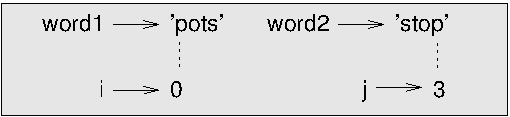
\includegraphics[scale = 0.8] {figs/state4.pdf}}
\caption{Diagrama de Estado.}
\label{} fig.state4
\end{figure}


Tomei um pouco de licença, organizando as variáveis ​​no quadro
e adição de linhas tracejadas para mostrar que os valores de {\tt i} e
{\tt j} indicam personagens em {\tt palavra1} e {\tt word2}.

\begin{} exercício
\label{} isreverse

A partir deste diagrama, executar o programa em papel, mudando o
valores de {\tt i} e {\tt j} durante cada iteração. Encontrar e corrigir o
segundo erro nesta função.

\end{} exercício



\section{} Glossário

\begin{description}

\item[objeto]: Algo uma variável pode consultar. Por agora,
você pode usar o `` objeto'' e `` valor'' alternadamente.
\index{objeto}

\item[seqüência:] um conjunto ordenado, isto é, um conjunto de
valores, onde cada valor é identificado por um índice inteiro.
\index{seqüência}

\item[Item]: Um dos valores em uma seqüência.
\index{artigo}

\item[índice]: Um valor inteiro usado para selecionar um item em
uma seqüência, como um caractere em uma string.
\index{index}

\item[fatia]: Uma parte de uma seqüência de caracteres especificada por uma série de índices.
\index{fatia}

\item[string vazia:] Uma string sem caracteres e comprimento 0, representado
por duas aspas.
\index{string vazio}

\item[imutável:] A propriedade de uma seqüência cujos itens não podem
ser atribuído.
\index{imutabilidade}

\item[travessia:] Para percorrer os itens em uma seqüência,
realizando uma operação semelhante em cada.
\index{travessia}

\item[busca]: Um padrão de travessia que pára
quando encontra o que está procurando.
\index{padrão de pesquisa}
\index{padrão! Pesquisa}

\item[contador]: A variável utilizada para contar alguma coisa, geralmente inicializado
a zero e então incrementada.
\index{counter}

\item[método:] Uma função que está associada a um objeto e chamado
usando a notação de ponto.
\index{método}

\item[invocação:] Uma declaração que chama um método.
\index{} invocação

\end{description}


\section{Exercícios}

\begin{} exercício
\index{size passo}
\index{operador de fatia}
\index{operador! Fatia}

Uma fatia corda pode levar um terceiro índice que especifica o passo ``
tamanho,'' ou seja, o número de espaços entre os caracteres sucessivos.
Um tamanho de passo de 2 significa qualquer outro personagem, 3 significa a cada três,
etc

\begin{verbatim}
>>> Fruta = 'banana'
>>> Fruta [00:05:02]
'Bnn'
\end{verbatim}

Um tamanho de passo de -1 atravessa a palavra para trás, de modo
a fatia \verb "[:: -1]" gera uma string invertida.
\index{palíndromo}

Use este idioma para escrever uma versão de uma linha de \verb "is_palindrome"
do Exercício ~ \ref {} palíndromo.
\end{} exercício


\begin{} exercício

As seguintes funções estão todos {\em destinar} para verificar se um
cadeia contém todas as letras minúsculas, mas pelo menos alguns deles são
errado. Para cada função, descreva o que a função realmente faz
(Assumindo que o parâmetro é uma string).

\begin{verbatim}
any_lowercase1 (s) def:
    para c em s:
        se c.islower ():
            retornar True
        else:
            retornará False

any_lowercase2 (s) def:
    para c em s:
        se 'c' islower ().:
            voltar 'True'
        else:
            voltar 'False'

any_lowercase3 (s) def:
    para c em s:
        flag = c.islower ()
    voltar bandeira

any_lowercase4 (s) def:
    flag = False
    para c em s:
        flag = bandeira ou c.islower ()
    voltar bandeira

any_lowercase5 (s) def:
    para c em s:
        se não c.islower ():
            retornará False
    retornar True
\end{verbatim}

\end{} exercício


\begin{} exercício
\index{rotação letter}
\index{rotação, letra}

\label{} exrotate
ROT13 é uma forma fraca de criptografia que envolve rotação ``'' cada
letra de uma palavra por 13 lugares. Para girar uma carta meio
para transferi-lo através do alfabeto, envolvendo em torno do início se
necessário, para "A" é deslocado por 3 'D' e 'Z' é desviado por um "A".

Escreva uma função chamada \verb "rotate_word"
que recebe uma string e um inteiro como parâmetros, e que os retornos
uma nova string que contém as letras da string original
``'' Rodado pela quantidade dada.  

Por exemplo, `` alegria'' girado por 7 é `` alegre'' e `` melão'' girada
por -10 é `` em cubos.''  

Por exemplo `` sono''
Girado por 9 é `` coelho'' e `` látex'' girado por 7 é `` xisto.''

Você pode querer usar as funções embutidas {\tt ord}, ​​que converte
um personagem de um código numérico, e {\tt chr}, ​​que converte numérico
códigos para caracteres.

Piadas potencialmente ofensivo na Internet são, por vezes, codificada
em ROT13. Se você não estiver facilmente ofendido, localizar e decodificar alguns
deles. Solução: \url{http://thinkpython.com/code/rotate.py}.

\end{} exercício


\chapter{Estudo de caso: jogo de palavras}

\section{Lendo listas de palavras}
\label{lista de palavras}

Para os exercícios deste capítulo, precisamos de uma lista de palavras em inglês.
Existem muitas listas de palavras disponíveis na Web, mas o mais
adequado para o nosso propósito é uma das listas de palavras coletadas e
contribuiu para o domínio público por Grady Ward como parte do Moby
projeto léxico (ver \url{http://wikipedia.org/wiki/Moby_Project}). Ele
é uma lista de 113.809 palavras cruzadas oficiais, ou seja, palavras que são
considerada válida nas palavras cruzadas e outros jogos de palavras. No
Coleção Moby, o nome do arquivo é {\tt 113809of.fic}; você pode baixar
uma cópia, com o nome simples {\tt words.txt}, a partir
\url{http://thinkpython.com/code/words.txt}.
\index{Moby Projeto}
\index{} palavras cruzadas

Este arquivo está em texto simples, para que você possa abri-lo com um texto
editor, mas você também pode lê-lo do Python. A built-in
função {\tt aberto} leva o nome do arquivo como um parâmetro
e retorna um arquivo {\bf objeto} pode ser usado para ler o arquivo.
\index{function open}
\index{function! Open}
\index{text plain}
\index{text! Plain}
\index{objeto! Arquivo}
\index{file objeto}

\begin{verbatim}
>>> Fin = open ('words.txt')
>>> Print fin
<Open arquivo'words.txt', modo'r' em 0xb7f4b380>
\end{verbatim}
%
{\tt fin} é um nome comum para um objeto de arquivo usado para
entrada. Modo \verb "'r'" indica que este arquivo é aberto para
leitura (em oposição ao verbo \"'w'" para a escrita).
\{Método readline} índice
\index{método! Readline}

O objeto de arquivo fornece vários métodos para leitura, incluindo a
{\tt readline}, que lê caracteres a partir do arquivo
até chegar a uma nova linha e retorna o resultado como um
string:

\begin{verbatim}
>>> Fin.readline ()
'Aa \r \n'
\end{verbatim}
%
A primeira palavra nesta lista especial é `` aa'', que é uma espécie de
lava. A seqüência \verb "\r \n" representa dois espaços em branco,
um retorno de carro e uma nova linha, que separam esta palavra do
seguinte.

O objeto de arquivo mantém o controle de onde ele está no arquivo, de modo
se você chamar {\tt readline} novamente, você terá a seguinte palavra:

\begin{verbatim}
>>> Fin.readline ()
'Aah \r \n'
\end{verbatim}
%
A próxima palavra é `` aah'', que é um perfeitamente legítimo
palavra, então pare de me olhar assim.
Ou, se ele é o espaço em branco que está incomodando,
podemos nos livrar dele com o método string {tira \tt}:
\{Método strip} índice
\index{método! Strip}

\begin{verbatim}
>>> Linha = fin.readline ()
>>> Word = line.strip ()
>>> Palavra impressão
aahed
\end{verbatim}
%
Você também pode usar um objeto de arquivo como parte de uma {\tt for} loop.
Este programa lê {\tt words.txt} e imprime cada palavra, uma
por linha:
\index{function open}
\index{function! Open}

\begin{verbatim}
fin = open ('words.txt')
para a linha de fin:
    palavra = line.strip ()
    palavra impressão
\end{verbatim}
%

\begin{} exercício

Escreva um programa que lê {\tt words.txt} e imprime apenas o
palavras com mais de 20 caracteres (sem contar espaços).
\index{espaços}

\end{} exercício


\section{Exercícios}

Existem soluções para estes exercícios na próxima seção.
Você deve pelo menos tentar cada um antes de ler as soluções.

\begin{} exercício

Em 1939 Ernest Vincent Wright publicou um romance de 50.000 palavras chamado
{\Em Gadsby} que não contém a letra `` e''. Desde `` e'' é
a letra mais comum em Inglês, isso não é fácil de fazer.

De facto, é difícil construir um pensamento solitário sem usar
que o símbolo mais comum. É um processo lento no início, mas com cautela
e horas de treinamento você pode gradualmente ganhar facilidade.

Tudo bem, eu vou parar agora.

Escreva uma função chamada \verb "has_no_e" que retorna {\tt verdadeira} if
a palavra dada não tem a letra `` e'' nele.

Modifique o programa da seção anterior para imprimir apenas as palavras
que não têm `` E'' e de calcular a percentagem das palavras na lista
não têm `` e''.
\index{} lipogram

\end{} exercício


\begin{} exercício 

Escreva uma função chamada {\tt evita}
que tem uma palavra e uma seqüência de letras proibidas, e
que os retornos {\tt true} se a palavra não usar qualquer um dos proibido
letras.

Modifique o seu programa para solicitar que o usuário digite uma string
de proibido letras e, em seguida, imprimir o número de palavras que
não contêm qualquer um deles.
Você pode encontrar uma combinação de 5 cartas proibidas que
exclui o menor número de palavras?

\end{} exercício



\begin{} exercício

Escreva uma função chamada \verb "uses_only" que leva uma palavra e um
seqüência de letras, e que os retornos {\tt true} se a palavra contém
apenas letras na lista. Você pode fazer uma frase usando apenas o
letras {\tt acefhlo}? Outros que `` Hoe alfafa?''

\end{} exercício


\begin{} exercício 

Escreva uma função chamada \verb "uses_all" que leva uma palavra e um
seqüência de letras necessárias e que os retornos {\tt true} se a palavra
usa todas as cartas necessárias, pelo menos, uma vez. Quantas palavras estão lá
que usar todas as vogais {\tt aeiou}? Que tal {\tt aeiouy}?

\end{} exercício


\begin{} exercício

Escreva uma função chamada \verb "is_abecedarian" que os retornos
{\tt true} se as letras de uma palavra aparecem em ordem alfabética
(Letras duplas são ok).  
Quantas palavras abecedarian existem?

\index{} abecedarian

\end{} exercício


\begin{} exercício
\label{palíndromo}
A palíndromo é uma palavra que lê o mesmo
Para a frente e para trás, como `` rotador'' e `` meio-dia.''
Escreve uma função booleana chamada \verbo "is_palindrome" que
Recebe uma string como parâmetro e retorna {\tt true} se é
Um palíndromo.

Modifique o seu programa da seção anterior para imprimir tudo
Dos palíndromos na lista de palavras e, em seguida, imprimir o total de
Númerodos palíndromos.
\end{} exercício



\section{} Pesquisa
\index{padrão de pesquisa}
\index{padrão! Pesquisa}

Todos os exercícios da seção anterior tem algo
em comum, pois eles podem ser resolvidos com o padrão de pesquisa que vimos
na Seção ~ \ref {} encontrar. O exemplo mais simples é a seguinte:

\begin{verbatim}
has_no_e def (palavra):
    por carta na palavra:
        se letra == 'e':
            retornará False
    retornar True
\end{verbatim}
%
O {\tt for} circuito percorre os personagens {\tt palavra}. Se encontrarmos
a letra `` e'', podemos retornar imediatamente {\tt false}; caso contrário,
tem que ir para a próxima letra. Se sair do circuito normalmente, que
significa que não encontrou um `` e'', assim voltamos {\tt true}.
\index{travessia}

Remoção isso porque nós não vimos o operador in ainda.
\index{} no operador
\index{operador! In}

Você poderia escrever essa função de forma mais concisa usando o {\tt no}
Operador%, mas eu comecei com esta versão porque ela 
Demonstra a lógica do padrão de pesquisa.
\index{generalização}

{\tt evita} é uma versão mais geral de \verb "has_no_e", mas
tem a mesma estrutura:

\begin{verbatim}
def evita (word, proibido):
    por carta na palavra:
        se carta em proibido:
            retornará False
    retornar True
\end{verbatim}
%
Podemos voltar {\tt false} assim que encontrar uma carta proibido;
se chegarmos ao final do ciclo, voltamos {\tt true}.

\Verb "uses_only" é similar, exceto que o sentido da condição
se inverte:

\begin{verbatim}
def uses_only (word, disponível):
    por carta na palavra: 
        se a carta não disponível em:
            retornará False
    retornar True
\end{verbatim}
%
Em vez de uma lista de cartas proibidas, temos uma lista de disponíveis
letras. Se encontrarmos uma carta na palavra {\tt} que não está em
{\tt disponível}, podemos voltar {\tt false}.

\Verb "uses_all" é similar, exceto que inverter o papel
da palavra e da seqüência de letras:

\begin{verbatim}
def uses_all (word, obrigatório):
    por carta exigida: 
        se a carta não em palavras:
            retornará False
    retornar True
\end{verbatim}
%
Em vez de percorrer as letras em {palavra \tt}, o loop
atravessa as letras necessárias. Se nenhuma das cartas necessárias
não aparecem na palavra, podemos voltar {\tt false}.
\index{travessia}

Se você estivesse realmente pensar como um cientista da computação, você faria
ter reconhecido que \verb "uses_all" foi um exemplo de um
problema anteriormente resolvido, e você teria escrito:

\begin{verbatim}
def uses_all (word, obrigatório):
    voltar uses_only (obrigatório, word)
\end{verbatim}
%
Este é um exemplo de um método de desenvolvimento de programa chamado problema {\bf
reconhecimento}, o que significa que você reconhece o problema que você está
trabalhando como uma instância de um problema anteriormente resolvido, e aplicar um
solução anteriormente desenvolvidos.
\index{reconhecimento do problema}
\index{plano de desenvolvimento! Reconhecimento do problema}


\section{Looping com índices}
\index{looping! Com índices}
\index{index! Looping com}

Eu escrevi as funções na seção anterior com {\tt for}
laços, porque eu só precisava dos personagens nas cordas, eu não fiz
tem que fazer qualquer coisa com os índices.

Para \verb "is_abecedarian" temos que comparar letras adjacentes,
que é um pouco complicado com um {\tt for} loop:

\begin{verbatim}
def is_abecedarian (palavra):
    anterior = palavra [0]
    para c na palavra:
        se c <anterior:
            retornará False
        anteriores = c
    retornar True
\end{verbatim}


Uma alternativa é a
usar recursão:

\begin{verbatim}
def is_abecedarian (palavra):
    if len (palavra) <= 1:
        retornar True
    se a palavra [0]> palavra [1]:
        retornará False
    voltar is_abecedarian (palavra [1:])
\end{verbatim}

Outra opção é usar um {\tt enquanto} loop:

\begin{verbatim}
def is_abecedarian (palavra):
    i = 0
    enquanto i <len (palavra) -1:
        se a palavra [i +1] <palavra [i]:
            retornará False
        i = i 1
    retornar True
\end{verbatim}
%
O ciclo começa no {\tt i = 0} e termina quando {\tt i = len (palavra) -1}. Cada
iteração do loop, ele compara o $ i $ mil caracteres (que você pode
pensar em como o personagem atual) para o carácter $ i $ 1 ª (que você
pode pensar em como o próximo).

Se o próximo caractere é inferior (em ordem alfabética antes) a corrente
um, então nós descobrimos uma pausa na tendência abecedarian e
voltamos {\tt false}.

Se se chegar ao fim do ciclo, sem encontrar uma falha, então o
palavra passa no teste. Para convencer-se de que as extremidades do laço
corretamente, considere um exemplo como \verb "'frescura'." O
comprimento da palavra é 6, então
a última vez que o loop é executado é quando {\tt i} é 4, que é o
índice do segundo ao último personagem. Na última iteração,
ele compara o segundo ao último personagem para o último, que é
o que queremos.
\index{palíndromo}

Aqui está uma versão de \verb "is_palindrome" (ver
Exercício ~ \ref {palíndromo}) que usa dois índices, um começa no
começando e vai até, a outra começa no final e vai para baixo.

\begin{verbatim}
is_palindrome def (palavra):
    i = 0
    j = len (palavra) -1

    enquanto i <j:
        se a palavra [i] = palavra [j]:
            retornará False
        i = i 1
        j = j-1

    retornar True
\end{verbatim}

Ou, se você percebeu que este é um exemplo de um resolvidos anteriormente
problema, você poderia ter escrito:

\begin{verbatim}
is_palindrome def (palavra):
    voltar is_reverse (word, word)
\end{verbatim}
\index{reconhecimento do problema}
\index{plano de desenvolvimento! Reconhecimento do problema}

Supondo que você fez Exercício ~ \ref {} isreverse.


\section{} Depuração
\index{depuração}
\index{teste! É difícil}
\{} Programa de testes de índice

Testando programas é difícil. As funções neste capítulo são
relativamente fácil de testar, pois você pode verificar os resultados com a mão.
Mesmo assim, ele está em algum lugar entre difícil e impossível escolher um
conjunto de palavras que testar para todos os erros possíveis.

Tomando \verb "has_no_e" como um exemplo, há dois óbvio
casos, para verificar: palavras que têm um 'e' deve retornar {\tt false};
palavras que não deve retornar {\tt true}. Você não deve ter
dificuldades para chegar com um de cada.

Dentro de cada um dos casos, há algumas subcasos menos óbvias. Entre o
palavras que têm um `` e'', você deve testar as palavras com um `` e'' no
começo, o fim, e em algum lugar no meio. Você deve testar longo
palavras, palavras curtas e palavras muito curtas, como a cadeia vazia. O
cadeia vazia é um exemplo de uma {\bf caso especial}, que é uma das
os casos de não-óbvias em que os erros muitas vezes se escondem.
\index{case especial}

Além dos casos de teste que você gerar, você também pode testar
o seu programa com uma lista de palavras como {\tt words.txt}. Por varredura
a saída, você pode ser capaz de detectar erros, mas tenha cuidado:
você pode pegar um tipo de erro (palavras que não devem ser
incluídos, mas são) e não outro (palavras que devem ser incluídos,
mas não o são).

Em geral, o teste pode ajudar a encontrar erros, mas não é fácil
gerar um bom conjunto de casos de teste, e mesmo se você fizer isso, você não pode
ter certeza que seu programa está correto.
\index{teste! Ea ausência de erros}

De acordo com um cientista da computação lendário:

\begin{quote}
Ensaio de programas pode ser usada para mostrar a presença de erros, mas nunca
mostrar a sua ausência!

--- Edsger W. Dijkstra
\end{quote}
\index{Dijkstra, Edsger}


\section{} Glossário

\begin{description}

\[Objeto de arquivo:] Item Um valor que representa um arquivo aberto.
\index{file objeto}
\index{objeto! Arquivo}

\[Reconhecimento problema:] item A maneira de resolver um problema por
expressá-la como uma instância de um problema anteriormente resolvido.
\index{reconhecimento do problema}

\item[caso especial:] Um caso de teste que é atípica ou não-óbvio
(E menos provável de ser tratada corretamente).
\index{case especial}

\end{description}


\section{Exercícios}

\begin{} exercício
\index{Car Talk}
\index{} Puzzler
\index{letras duplas}

Esta questão é baseada em um quebra-cabeças que foi transmitido no rádio
programa {\em Car Talk} 
(\url{http://www.cartalk.com/content/puzzlers}):

\begin{quote}
Dê-me uma palavra com três letras duplas consecutivas. Vou te dar um
duas palavras que quase se qualificar, mas não o fazem. Por exemplo, a palavra
comitê, comitê. Seria ótimo, exceto para o `i 'que
foge lá. Ou Mississippi: Mississippi. Se você pudesse
tirar aqueles que eu de que iria funcionar. Mas há uma palavra que tem três
pares consecutivos de letras e para o melhor de meu conhecimento, este pode
ser a única palavra. Claro que há, provavelmente, mais de 500, mas só posso
pensar em um. Qual é a palavra?
\end{quote}

Escreva um programa para encontrá-lo. Solução: \url{http://thinkpython.com/code/cartalk1.py}.

\end{} exercício


\begin{} exercício
Aqui está outro {\em Car Talk}
Puzzler (\url{http://www.cartalk.com/content/puzzlers}):
\index{Car Talk}
\index{} Puzzler
\index{} odômetro
\index{palíndromo}

\begin{quote}
`` Eu estava dirigindo na estrada no outro dia e aconteceu de eu
notar meu odômetro. Como a maioria dos odômetros, mostra seis dígitos,
em milhas inteiras só. Então, se meu carro tinha 300.000
milhas, por exemplo, eu veria 3-0-0-0-0-0.

`` Agora, o que eu vi naquele dia foi muito interessante. Notei que o
4 últimos algarismos eram palíndromo, ou seja, eles lêem o mesmo para a frente como
para trás. Por exemplo, 5-4-4-5 é um palíndromo, então meu odômetro
poderia ter lido 3-1-5-4-4-5.

`` Um quilômetro depois, os últimos 5 números foram palíndromo. Por exemplo, ele
poderia ter lido 3-6-5-4-5-6. Um quilômetro depois, no meio de 4 de
6 números foram palíndromo. E você está pronto para isso? Um quilômetro depois,
todas as 6 foram palíndromo!

`` A questão é, o que era no hodômetro quando eu olhei pela primeira vez?''
\end{quote}

Escreva um programa Python que testa todos os números de seis dígitos e estampas
quaisquer números que satisfazem esses requisitos.  
Solução: \url{http://thinkpython.com/code/cartalk2.py}.

\end{} exercício


\begin{} exercício
Aqui está outro {\em Car Talk} Puzzler você pode resolver com um
pesquisa (\url{http://www.cartalk.com/content/puzzlers}):
\index{Car Talk}
\index{} Puzzler
\index{palíndromo}

\begin{quote}
`` Recentemente eu tive uma visita com a minha mãe e nós percebemos que
os dois dígitos que compõem a minha idade quando revertida resultou em sua
idade. Por exemplo, se ela é 73, eu sou 37. Nós nos perguntamos quantas vezes isso tem
aconteceu ao longo dos anos, mas nós temos desviado com outros temas e
nunca veio com uma resposta.

`` Quando cheguei em casa eu descobri que os dígitos de nossas idades foram
reversíveis seis vezes até agora. Eu também descobri que, se tivermos sorte ela
voltaria a acontecer em poucos anos, e se tiver muita sorte que seria
acontecer mais uma vez depois disso. Em outras palavras, ele teria
aconteceu 8 vezes sobre tudo. Então a questão é, quantos anos eu estou agora?''

\end{quote}

Escreva um programa Python que procura por soluções para este enigma.
Dica: você pode encontrar o método string {\tt zfill} útil.

Solução: \url{http://thinkpython.com/code/cartalk3.py}.

\end{} exercício



\chapter{Listas}

\section{A lista é uma seqüência}
\label{seqüência}

Como uma corda, uma lista {\bf} é uma seqüência de valores. Em uma string, a
Os valores são caracteres; numa lista, que pode ser de qualquer tipo. Os valores
uma lista são chamados elementos {\bf} ou às vezes {itens \bf}.
\index{lista}
\index{type! Lista}
\index{element}
\index{seqüência}
\index{artigo}

Existem várias maneiras de criar uma nova lista, o mais simples é
envolver os elementos em colchetes (\verb "[" e \verb "]"):

\begin{verbatim}
[10, 20, 30, 40]
['Sapo crocante "," bexiga carneiro', 'vômito cotovia']
\end{verbatim}
%
O primeiro exemplo é uma lista de quatro inteiros. O segundo é uma lista de
três cordas. Os elementos de uma lista não precisa ser do mesmo tipo.
A lista a seguir contém uma string, um float, um inteiro e
(Lo!) outra lista:

\begin{verbatim}
['Spam', 2,0, 5, [10, 20]]
\end{verbatim}
%
Uma lista dentro de outra lista é {\bf aninhada}.
\index{lista aninhada}
\index{list! Aninhada}

Uma lista que não contém nenhum elemento é
chamado de uma lista vazia, você pode criar um com vazio
colchetes, \verb "[]".
\index{lista vazia}
\index{list! Vazio}

Como você poderia esperar, você pode atribuir valores de lista de variáveis:

\begin{verbatim}
>>> Queijos = ['Cheddar', 'Edam', 'Gouda']
>>> Números = [17, 123]
>>> = Vazios []
>>> Queijos de impressão, números, vazio
['Cheddar', 'Edam', 'Gouda'] [17, 123] []
\end{verbatim}
%
\index{atribuição}


\section {} Listas são mutáveis
\label{} mutável
\index{list! Elemento}
\index{acesso}
\index{index}
\index{operador colchete}
\index{operador! Suporte}

A sintaxe para o acesso aos elementos de uma lista é o mesmo que para
acessar os caracteres de uma string --- o operador suporte. O
expressão dentro dos colchetes especifica o índice. Lembre-se que o
índices iniciam em 0:

\begin{verbatim}
>>> Print queijos [0]
Queijo Cheddar
\end{verbatim}
%
Ao contrário de cordas, as listas são mutáveis. Quando o operador colchete aparece
no lado esquerdo de uma atribuição, ele identifica o elemento do
lista que será atribuído.
\index{} mutabilidade

\begin{verbatim}
>>> Números = [17, 123]
>>> Números [1] = 5
>>> números de impressão
[17, 5]
\end{verbatim}
%
O elemento de um eth de números {\tt}, que
utilizado para ser 123, é agora 5.
\index{index! Começando em zero}
\index{zero, índice a partir de}

Você pode pensar em uma lista como uma relação entre os índices e
elementos. Essa relação é chamada de mapeamento {\bf}; cada índice
`` Mapeia para'' um dos elementos. Figura ~ \ref {} fig.liststate espetáculos
o diagrama de estado para {\tt
queijos}, {números \tt} e {\tt vazio}:
\index{diagrama de estado}
\index{diagrama! Estado}
\index{mapeamento}

\begin{figure}
\centerline
{\includegraphics[scale = 0.8] {figos / liststate.pdf}}
\caption{Diagrama de Estado.}
\label{} fig.liststate
\end{figure}

As listas são representados por caixas com a palavra `` lista'' fora
e os elementos da lista de dentro. {Queijos \tt} refere-se a
uma lista com três elementos indexados 0, 1 e 2.
{Números \tt} contém dois elementos, o diagrama mostra que o
valor do segundo elemento foi transferido 123-5.
{\tt vazio} refere-se a uma lista com nenhum elemento.
\{} Atribuição item de índice
\index{atribuição! Artigo}

Índices lista de trabalho da mesma forma que os índices de string:

\begin{itemize}

\item Qualquer expressão inteiro pode ser usado como um índice.

\item Se você tentar ler ou escrever um elemento que não existe, você
obter uma {\tt IndexError}.
\index{exceção! IndexError}
\index{} IndexError

\item Se um índice possui um valor negativo, ele conta ao contrário do
fim da lista.

\end{itemize}
\index{list! Index}

\index{list! Adesão}
\index{adesão! Lista}
\index{} no operador
\index{operador! In}

O {\tt no} operador também funciona em listas.

\begin{verbatim}
>>> Queijos = ['Cheddar', 'Edam', 'Gouda']
>>> 'Edam' em queijos
Verdadeiro
>>> 'Brie' em queijos
Falso
\end{verbatim}


\section{Atravessando uma lista}
\index{list! Travessia}
\index{travessia! Lista}
\index{loop}
\index{laço! For}
\index{declaração! For}

A forma mais comum de atravessar os elementos de uma lista é
com uma {\tt for} loop. A sintaxe é a mesma que para strings:

\begin{verbatim}
para o queijo em queijos:
    queijo impressão
\end{verbatim}
%
Isso funciona bem se você só precisa ler os elementos do
lista. Mas se você quer escrever ou atualizar os elementos, você
precisa dos índices. Uma maneira comum de fazer isso é combinar
as funções {range \tt} e {\tt len}:
\index{looping! Com índices}
\index{index! Looping com}

\begin{verbatim}
for i in range (len (números)):
    números [i] = números [i] * 2
\end{verbatim}
%
Este loop percorre a lista e atualiza cada elemento. {\tt len}
devolve o número de elementos na lista. {range \tt} retornos
uma lista de índices de 0 a n-1 $ $, onde $ n $ é o comprimento de
lista. Cada vez através do loop {\tt i} obtém o índice
do próximo elemento. A instrução de atribuição nos usos do corpo
{\tt i} para ler o valor antigo do elemento e para atribuir o
novo valor.
\{Update} item de índice
\index{update! Artigo}

A {\tt for} loop sobre uma lista vazia nunca executa o corpo:

\begin{verbatim}
para x em []:
    imprimir "Isso nunca acontece."
\end{verbatim}
%
Apesar de uma lista pode conter outra lista, a aninhados
lista ainda conta como um único elemento. O comprimento desta lista é
quatro:
\index{lista aninhada}
\index{list! Aninhada}

\begin{verbatim}
['Spam', 1, ['Brie', 'Roquefort', 'Pol le Veq'], [1, 2, 3]]
\end{verbatim}



\{} Operações Lista de seção
\index{list! Operação}

O {\tt +} concatena listas:
\index{concatenação! Lista}
\index{list! Concatenação}

\begin{verbatim}
>>> A = [1, 2, 3]
>>> B = [4, 5, 6]
>>> C = a + b
>>> Print c
[1, 2, 3, 4, 5, 6]
\end{verbatim}
%
Da mesma forma, o {\tt *} operador repete uma lista um determinado número de vezes:
\index{repetição! Lista}
\index{list! Repetição}

\begin{verbatim}
>>> [0] * 4
[0, 0, 0, 0]
>>> [1, 2, 3] * 3
[1, 2, 3, 1, 2, 3, 1, 2, 3]
\end{verbatim}
%
O primeiro exemplo repete {\tt [0]} quatro vezes. O segundo exemplo
repete a lista {\tt [1, 2, 3]} três vezes.


\section{Lista fatias}
\index{operador de fatia}
\index{operador! Fatia}
\index{index! Fatia}
\index{list! Fatia}
\index{fatia! Lista}

O operador de fatia também funciona em listas:

\begin{verbatim}
>>> T = ['a', 'b', 'c', 'd', 'e', ​​'f']
>>> T [01:03]
['B', 'c']
>>> T [: 4]
['A', 'b', 'c', 'd']
>>> T [3]:
['D', 'e', ​​'f']
\end{verbatim}
%
Se você omitir o primeiro índice, a fatia começa no início.
Se você omitir o segundo, a fatia vai para o fim. Então, se você
omitir ambos, a fatia é uma cópia de toda a lista.
\index{list! Cópia}
\index{fatia! Cópia}
\index{cópia! Fatia}

\begin{verbatim}
>>> T [:]
['A', 'b', 'c', 'd', 'e', ​​'f']
\end{verbatim}
%
Desde as listas são mutáveis, muitas vezes é útil fazer uma cópia
antes que as operações que se dobram, eixo ou mutilam realizando
listas.
\index{} mutabilidade

Um operador de fatia no lado esquerdo de uma atribuição
pode atualizar vários elementos:
\index{fatia! Update}
\index{update! Fatia}

\begin{verbatim}
>>> T = ['a', 'b', 'c', 'd', 'e', ​​'f']
>>> T [01:03] = ['x', 'y']
>>> Print t
['A', 'x', 'y', 'd', 'e', ​​'f']
\end{verbatim}
%

Você pode adicionar elementos a uma lista de espremê-los em um vazio
Fatia:

%\begin{verbatim}
>>> T = ['a', 'd', 'e', ​​'f']
>>> T [01:01] = ['b', 'c']
>>> Print t
['A', 'b', 'c', 'd', 'e', ​​'f']
\end{verbatim}
\afterverb
%
E você pode remover elementos de uma lista atribuindo a lista vazia para
Deles:

%\begin{verbatim}
>>> T = ['a', 'b', 'c', 'd', 'e', ​​'f']
>>> T [01:03] = []
>>> Print t
['A', 'd', 'e', ​​'f']%
\end{verbatim}
\afterverb
%
Mas ambosdessas operações podem ser expressas de forma mais clara
Com os métodos da lista.


\{} Lista de métodos de seção
\index{list! Método}
\index{método, lista}

Python fornece métodos que operam sobre listas. Por exemplo,
{\tt} append adiciona um novo elemento ao final de uma lista:
\index{método append}
\index{método! Append}

\begin{verbatim}
>>> T = ['a', 'b', 'c']
>>> T.append ('d')
>>> Print t
['A', 'b', 'c', 'd']
\end{verbatim}
%
{\tt estender} pega uma lista como um argumento e acrescenta todos
os elementos:
\index{método estender}
\index{método! Estender}

\begin{verbatim}
>>> T1 = ['a', 'b', 'c']
>>> T2 = ['d', 'e']
>>> T1.extend (t2)
>>> T1 impressão
['A', 'b', 'c', 'd', 'e']
\end{verbatim}
%
Este exemplo folhas {\tt} t2 não modificado.

{\tt tipo} organiza os elementos da lista de baixo para cima:
\{} Método de classificação do índice
\index{método! Tipo}

\begin{verbatim}
>>> T = ['d', 'c', 'e', ​​'b', 'a']
>>> T.sort ()
>>> Print t
['A', 'b', 'c', 'd', 'e']
\end{verbatim}
%
Métodos de lista são todos nulos, eles modificar a lista e retornar {\tt Nenhum}.
Se você acidentalmente escrever {\tt t = t.sort ()}, você vai se decepcionar
com o resultado.
\index{método vazio}
\index{método! Vazio}
\index{Nenhum valor especial}
\index{valor especial! Nenhum}


\section{Map, filtro e reduzir}

Para somar todos os números em uma lista, você pode usar um loop assim:

Ver add.py

\begin{verbatim}
add_all def (t):
    Total = 0
    para x em t:
        total de + = x
    retorno total
\end{verbatim}
%
{\tt totais} é inicializado em 0. Cada vez através do loop,
{\tt x} recebe um elemento da lista. O {\tt + = operador}
fornece uma maneira curta para atualizar uma variável. Este
{\bf instrução de atribuição aumentada}:
\index{operador update}
\index{operador! Update}
\index{atribuição! Aumentada}
\index{atribuição aumentada}

\begin{verbatim}
    total de + = x
\end{verbatim}
%
é equivalente a:

\begin{verbatim}
    total = total + x
\end{verbatim}
%
À medida que o ciclo executa, {\tt totais} acumula a soma do
elementos; uma variável usada desta forma é às vezes chamado de
{\bf acumulador}.
\index{acumulador! Soma}

Somando-se os elementos de uma lista é uma operação tão comum
que Python oferece-lo como uma função interna, {soma \tt}:

\begin{verbatim}
>>> T = [1, 2, 3]
>>> Soma (t)
6
\end{verbatim}
%
Uma operação como esta, que combina uma sequência de elementos em
um único valor é às vezes chamado {\bf reduzir}.
\index{reduzir padrão}
\index{padrão! Reduzir}
\index{travessia}

\begin{} exercício

Escreva uma função chamada \verb "nested_sum" que leva uma lista aninhada
de números inteiros e somar os elementos de todas as listas aninhadas.

\end{} exercício

Às vezes você quer atravessar uma lista, enquanto a construção
outro. Por exemplo, a seguinte função recebe uma lista de strings
e retorna uma nova lista que contém seqüências de letras maiúsculas:

\begin{verbatim}
capitalize_all def (t):
    res = []
    para s em t:
        res.append (s.capitalize ())
    voltar res
\end{verbatim}
%
{Res \tt} é inicializada com uma lista vazia; cada vez através
o loop, nós adicionamos o próximo elemento. Então {res \tt} é outra
tipo de acumulador.
\index{acumulador! Lista}

Uma operação como \verb "capitalize_all" é às vezes chamado de {\bf
mapa} porque `` mapas'' uma função (neste caso o método de {\tt
capitalizar}) para cada um dos elementos em uma seqüência.
\index{padrão mapa}
\index{padrão! Mapa}
\index{padrão de filtro}
\index{padrão! Filtro}

\begin{} exercício

Use \verb "capitalize_all" para escrever uma função chamada \verb "capitalize_nested"
que leva uma lista aninhada de strings e retorna uma nova lista aninhada
com todas as strings em maiúsculas.

\end{} exercício

Outra operação comum é selecionar alguns dos elementos de
uma lista e retornar uma sublista. Por exemplo, a seguir
função recebe uma lista de strings e retorna uma lista que contém
apenas as seqüências de letras maiúsculas:

\begin{verbatim}
def only_upper (t):
    res = []
    para s em t:
        se s.isupper ():
            res.append (s)
    voltar res
\end{verbatim}
%
{\tt isupper} é um método string que retorna {\tt verdadeira} if
a string contém apenas letras maiúsculas.

Uma operação como \verb "only_upper" é chamado de filtro {\bf} porque
selecciona alguns dos elementos e filtros para fora dos outros.

Operações de lista mais comuns pode ser expressa como uma combinação
do mapa, filtrar e reduzir. Como essas operações são
tão comum, Python fornece recursos de linguagem para apoiá-los,
incluindo a função built-in {\tt mapa} e um operador
chamado de `` compreensão da lista''.
\index{list! Compreensão}

\begin{} exercício
\label{} cumulativo
\index{soma cumulativa}

Escrever uma função que recebe uma lista de números e retorna o
soma cumulativa, isto é, uma nova lista onde o $ i $ ésimo elemento
é a soma da primeira $ i $ 1 elementos da lista original.
Por exemplo, a soma cumulativa de {\tt [1, 2, 3]} é
{\tt [1, 3, 6]}. 
\end{} exercício


\section{Excluindo elementos}
\index{elemento exclusão}
\index{exclusão, elemento da lista}

Existem várias formas de eliminar os elementos de uma lista. Se você
saber o índice do elemento que você quiser, você pode usar
{\tt pop}:
\{Método pop} índice
\index{método! Pop}

\begin{verbatim}
>>> T = ['a', 'b', 'c']
>>> X = t.pop (1)
>>> Print t
['A', 'c']
>>> Print x
b
\end{verbatim}
%
{\tt pop} modifica a lista e retorna o elemento que foi removido.
Se você não fornecer um índice, que exclui e retorna o
último elemento.

Se você não precisa do valor removido, você pode usar o {\tt del}
operador:
\index{del operador}
\index{operador! Del}

\begin{verbatim}
>>> T = ['a', 'b', 'c']
>>> Del t [1]
>>> Print t
['A', 'c']
\end{verbatim}
%

Se você sabe que o elemento que você deseja remover (mas não o índice), você
pode usar {\tt remove}:
\index{remover método}
\index{método remove!}

\begin{verbatim}
>>> T = ['a', 'b', 'c']
>>> T.remove ('b')
>>> Print t
['A', 'c']
\end{verbatim}
%
O valor de retorno {\tt remove} é {\tt Nenhum}.
\index{Nenhum valor especial}
\index{valor especial! Nenhum}

Para remover mais de um elemento, você pode usar {\tt del} com
um índice de fatia:

\begin{verbatim}
>>> T = ['a', 'b', 'c', 'd', 'e', ​​'f']
>>> Del t [01:05]
>>> Print t
['A', 'f']
\end{verbatim}
%
Como de costume, a fatia seleciona todos os elementos até, mas não
incluindo, o segundo índice.

\begin{} exercício

Escreva uma função chamada \verb "meio" que leva uma lista e
retorna uma nova lista que contém todos, mas o primeiro e último
elementos. Então \"meio ([1,2,3,4])" verbo deve retornar \verb "[2,3]".

\end{} exercício

\begin{} exercício

Escreva uma função chamada \verb "chop" que leva uma lista, modifica-lo
removendo os primeiros e últimos elementos, e retorna {\tt Não}.

\end{} exercício


\section{Listas e strings}
\index{lista}
\index{string}
\index{seqüência}

Uma string é uma sequência de caracteres e uma lista é uma seqüência
de valores, mas de uma lista de caracteres não é a mesma como um
string. Para converter uma string para uma lista de caracteres,
você pode usar {list \tt}:
\index{list! Função}
\index{function! Lista}

\begin{verbatim}
>>> S = 'spam'
>>> T = lista (s)
>>> Print t
['S', 'p', 'a', 'm']
\end{verbatim}
%
Porque {tt lista \} é o nome de uma função built-in, você deve
evite usá-lo como um nome de variável. Eu também evitar {\tt l} porque
ele parece muito com o {\tt 1}. Então é por isso que eu uso {\tt t}.

A lista {\tt} function quebra uma string em letras individuais. Se
você quer quebrar uma string em palavras, você pode usar o {\tt divisão}
Método:
\{Método split} índice
\index{método! Divisão}

\begin{verbatim}
>>> S = 'ansiando para os fiordes "
>>> T = s.split ()
>>> Print t
['Definhando', 'para', 'a', 'fiordes']
\end{verbatim}
%
Um argumento opcional chamado um delimitador {\bf} especifica que
caracteres para usar como limites da palavra.
O exemplo a seguir
usa um hífen como um delimitador:
\index{argumento opcional}
\index{argumento! Opcional}
\index{delimitador}

\begin{verbatim}
>>> S = 'spam-spam-spam'
>>> Delimitador = '-'
>>> S.split (delimitador)
["Spam", "spam", "spam"]
\end{verbatim}
%
{\tt juntar} é o inverso de {\tt dividida}. Ele
toma uma lista de strings e
concatena os elementos. {\tt juntar} é um método de corda,
então você tem que chamá-lo sobre o delimitador e passar a
listar como um parâmetro:
\index{método join}
\index{método! Juntar}
\index{concatenação}

\begin{verbatim}
>>> T = ['definhando', 'para', 'a', 'fiordes']
>>> Delimitador = ''
>>> Delimiter.join (t)
'Ansiando para os fiordes "
\end{verbatim}
%
Neste caso, o delimitador é um caractere de espaço, de modo
{\tt juntar} coloca um espaço entre as palavras. Para concatenar
cordas, sem espaços, você pode usar a cadeia vazia,
\Verb "''", como um delimitador. 
\index{string vazio}
\index{string! Vazio}


\section {Objetos e valores}
\index{objeto}
\index{value}

Se nós executarmos estas instruções de atribuição:

\begin{verbatim}
a = 'banana'
b = 'banana'
\end{verbatim}
%
Sabemos que {\tt a} e {\tt b} tanto se referir a um
corda, mas não temos
saber se eles se referem ao {\em mesmo} string.
Existem dois estados possíveis, mostrados na Figura ~ \ref {fig.list1}.
\index{aliasing}

\begin{figure}
\centerline
{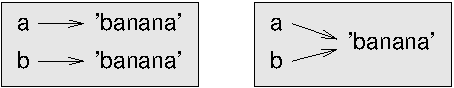
\includegraphics[scale = 0.8] {figs/list1.pdf}}
\caption{Diagrama de Estado.}
\label{} fig.list1
\end{figure}


Em um caso, {\tt a} e {\tt b} se referem a dois objectos diferentes que
tem o mesmo valor. No segundo caso, eles se referem à mesma
objeto.
\index{} é a operadora
\index{operador! É}

Para verificar se duas variáveis ​​se referem ao mesmo objeto, você pode
usar o {\tt é} operador.

\begin{verbatim}
>>> A = 'banana'
>>> B = 'banana'
>>> A é b
Verdadeiro
\end{verbatim}
%
Neste exemplo, apenas Python criou um objeto string,
e ambos {\tt a} e {\tt b} se referem a ele.

Mas quando você cria duas listas, você tem dois objetos:

\begin{verbatim}
>>> A = [1, 2, 3]
>>> B = [1, 2, 3]
>>> A é b
Falso
\end{verbatim}
%
Assim, o diagrama de estado se parece com a Figura ~ \ref {} fig.list2.
\index{diagrama de estado}
\index{diagrama! Estado}

\begin{figure}
\centerline
{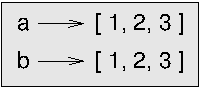
\includegraphics[scale = 0.8] {figs/list2.pdf}}
\caption{Diagrama de Estado.}
\label{} fig.list2
\end{figure}


Neste caso, diríamos que as duas listas são {\bf equivalente},
porque eles têm os mesmos elementos, mas não {\bf idêntico}, porque
eles não são o mesmo objeto. Se dois objetos são idênticos, eles são
Também equivalente, mas se eles são equivalentes, eles não são necessariamente
idêntico.
\index{equivalência}
\index{identidade}

Até agora, temos sido objeto usando ``'' e `` valor''
como sinônimos, mas é mais preciso dizer que um objeto tem uma
valor. Se você executar {\tt [1,2,3]}, você recebe uma lista
objeto cujo valor é uma seqüência de números inteiros. Se outro
lista tem os mesmos elementos, dizemos que ela tem o mesmo valor, mas
não é o mesmo objecto.
\index{objeto}
\index{value}


\section{} Aliasing
\index{aliasing}
\index{referência! Aliasing}

Se {\tt a} refere-se a um objeto e você atribui {\tt b = a},
em seguida, ambas as variáveis ​​se referem ao mesmo objeto:

\begin{verbatim}
>>> A = [1, 2, 3]
>>> B = a
B é um >>>
Verdadeiro
\end{verbatim}
%
O diagrama de estado se parece com a Figura ~ \ref {} fig.list3.
\index{diagrama de estado}
\index{diagrama! Estado}

\begin{figure}
\centerline
{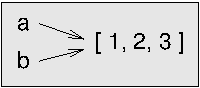
\includegraphics[scale = 0.8] {figs/list3.pdf}}
\caption{Diagrama de Estado.}
\label{} fig.list3
\end{figure}

A associação de uma variável com um objeto é chamado de {\bf
referência}. Neste exemplo, há duas referências à mesma
objeto.
\index{referência}

Um objeto com mais de uma referência tem mais
de um nome, por isso dizemos que o objeto é {\bf alias}.
\index{} mutabilidade

Se o objeto alias é mutável, as alterações feitas com um apelido afetam
o outro:

\begin{verbatim}
>>> B [0] = 17
>>> Print um
[17, 2, 3]
\end{verbatim}
%
Embora este comportamento possa ser útil, é passível de erro. Em geral,
é mais seguro para evitar aliasing quando você está trabalhando com mutável
objetos.
\index{imutabilidade}

Para objetos imutáveis, como cordas, aliasing não é tanto de uma
problema. Neste exemplo:

\begin{verbatim}
a = 'banana'
b = 'banana'
\end{verbatim}
%
Ele quase nunca faz diferença se {\tt a} e {\tt b} se referem
para a mesma cadeia ou não.


\{} Lista de argumentos seção
\label{} list.arguments
\index{list! Como argumento}
\index{argumento}
\index{argumento! Lista}
\index{referência}
\index{parâmetro}

Quando você passar uma lista para uma função, a função obtém uma referência
à lista.
Se a função modifica um parâmetro da lista, o chamador vê a mudança.
Por exemplo, \verb "delete_head" remove o primeiro elemento de uma lista:

\begin{verbatim}
delete_head def (t):
    del t [0]
\end{verbatim}
%
Aqui está como ele é usado:

\begin{verbatim}
>>> Letras = ['a', 'b', 'c']
>>> Delete_head (letras)
>>> cartas de impressão
['B', 'c']
\end{verbatim}
%
O parâmetro {\tt t} e {a variável letras \tt} são
apelidos para o mesmo objeto. O diagrama de pilha
Figura ~ \ref {} fig.stack5.
\index{diagrama de pilha}
\index{diagrama! Pilha}

\begin{figure}
\centerline
{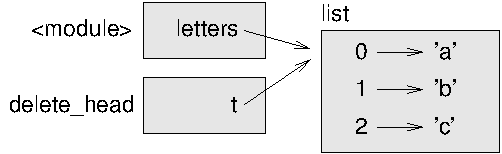
\includegraphics[scale = 0.8] {figs/stack5.pdf}}
\caption{diagrama Stack.}
\label{} fig.stack5
\end{figure}


Como a lista é compartilhada por dois quadros, que eu desenhei
entre eles.

É importante distinguir entre as operações que
modificar listas e operações que criam novas listas. Para
exemplo, o {\tt} append método modifica uma lista, mas o
{\tt +} operador cria uma nova lista:
\index{método append}
\index{método! Append}
\index{list! Concatenação}
\index{concatenação! Lista}

\begin{verbatim}
>>> T1 = [1, 2]
>>> T2 = t1.append (3)
>>> T1 impressão
[1, 2, 3]
>>> Print t2
Nenhum

>>> T3 = t1 + [4]
>>> Print t3
[1, 2, 3, 4]
\end{verbatim}

Essa diferença é importante quando você escrever funções que
devem modificar listas. Por exemplo, esta função
{\Em não apagar} a cabeça de uma lista:

\begin{verbatim}
bad_delete_head def (t):
    t = t [1:] # ERRADO!
\end{verbatim}

O operador de fatia cria uma nova lista ea atribuição
faz {\tt t} se referem a ele, mas nada disso tem qualquer efeito
na lista que foi passada como argumento.
\index{operador de fatia}
\index{operador! Fatia}

Uma alternativa é escrever uma função que cria e
retorna uma nova lista. Para
exemplo, {\tt cauda} retorna todos, mas o primeiro
elemento de uma lista:

\begin{verbatim}
cauda def (t):
    retornar t [1:]
\end{verbatim}
%
Esta função deixa a lista original não modificado.
Aqui está como ele é usado:

\begin{verbatim}
>>> Letras = ['a', 'b', 'c']
>>> Resto = cauda (letras)
>>> Resto impressão
['B', 'c']
\end{verbatim}



\section{} Depuração
\index{depuração}

O uso descuidado de listas (e outros objetos mutáveis)
pode levar a longas horas de depuração. Aqui estão alguns comum
armadilhas e maneiras de evitá-los:

\begin{enumerate}

\item Não se esqueça que a maioria dos métodos lista modificar o argumento e
  voltar {\tt Nenhum}. Isto é o oposto dos métodos de cordas,
  que retornar uma nova string e deixar o original em paz.

Se você está acostumado a escrever código string como esta:

\begin{verbatim}
palavra = word.strip ()
\end{verbatim}

É tentador escrever código lista como esta:

\begin{verbatim}
t = t.sort () # ERRADO!
\end{verbatim}
\{} Método de classificação do índice
\index{método! Tipo}

Porque {\tt Colecção} retorna {\tt none}, o
próxima operação de executar com {\tt t} é provável que falhe.

Antes de utilizar métodos e operadores de lista, você deve ler o
documentação com cuidado e, em seguida, testá-los no modo interativo. O
métodos e operadores que listas de compartilhamento com outras seqüências (como
cordas) estão documentadas em
\url{http://docs.python.org/2/library/stdtypes.html # typesseq}. O
métodos e operadores que se aplicam apenas a seqüências mutáveis
são documentados em \url{http://docs.python.org/2/library/stdtypes.html # typesseq-mutável}.


\item Escolha um idioma e ficar com ela.

Parte do problema com as listas é que há muitos
maneiras de fazer as coisas. Por exemplo, para remover um elemento
uma lista, você pode usar {\tt pop}, {\tt remove}, {\tt del},
ou até mesmo uma atribuição fatia.

Para adicionar um elemento, você pode usar o {\tt} append método ou
o {\tt +} operador. Supondo-se que {\tt t} é uma lista e
{\tt x} é um elemento da lista, estes são a direita: 

\begin{verbatim}
t.append (x)
t = t + [x]
\end{verbatim}

E estes estão errados:

\begin{verbatim}
t.append ([x]) # ERRADO!
t = t.append (x) # ERRADO!
t + [x] # ERRADO!
t = t + x # ERRADO!
\end{verbatim}

Experimente cada um desses exemplos no modo interativo para certificar-se
Você entende o que eles fazem. Note-se que apenas a última
um faz com que um erro de execução, os outros três são legais, mas eles
fazer a coisa errada.


\item Faça cópias para evitar aliasing.
\index{aliasing! Cópia para evitar}
\index{cópia! Para evitar aliasing}

Se você quiser usar um método como {\tt tipo} que modifica
o argumento, mas você precisa para manter a lista original, como
bem, você pode fazer uma cópia.

\begin{verbatim}
orig = t [:]
t.sort ()
\end{verbatim}

Neste exemplo, você também pode usar a função built-in {\tt classificadas},
que retorna uma lista nova, classificado e deixa o original sozinho.
Mas, nesse caso, você deve evitar o uso de {\tt classificadas} como uma variável
nomear!

\end{enumerate}



\section{} Glossário

\begin{description}

\item[lista]: A seqüência de valores.
\index{lista}

\item[elemento:] Um dos valores em uma lista (ou outra seqüência),
também chamado itens.
\index{element}

\item[índice]: Um valor inteiro que indica um elemento em uma lista.
\index{index}

\item[lista aninhada:] Uma lista que é um elemento de uma outra lista.
\index{lista aninhada}

\item[list travessia:] O acessando seqüencial de cada elemento em uma lista.
\index{list! Travessia}

\item[mapeamento]: uma relação em que cada elemento de um conjunto
corresponde a um elemento de um outro conjunto. Por exemplo, uma lista é
um mapeamento de índices para os elementos.
\index{mapeamento}

\item[acumulador:] Uma variável usada em um loop para somar ou
acumular um resultado.
\index{acumulador}

\item[aumentada atribuição:] Uma declaração de que atualiza o valor
de uma variável usando um operador como \verb "+ =".
\index{atribuição! Aumentada}
\index{atribuição aumentada}
\index{travessia}

\item[reduzir]: Um padrão de processamento que atravessa uma seqüência 
e acumula os elementos em um único resultado.
\index{reduzir padrão}
\index{padrão! Reduzir}

\item[mapa]: Um padrão de processamento que atravessa uma seqüência e
realiza uma operação em cada elemento.
\index{padrão mapa}
\index{padrão! Mapa}

\item[filtro]: Um padrão de processamento que atravessa uma lista e
seleciona os elementos que satisfazem algum critério.
\index{padrão de filtro}
\index{padrão! Filtro}

\item[objeto]: Algo uma variável pode consultar. Um objeto
tem um tipo e um valor.
\index{objeto}

\item[equivalente:] com o mesmo valor.
\index{equivalente}

\item[idênticas:] Sendo o mesmo objeto (o que implica equivalência).
\index{idêntico}

\item[referência:] A associação entre uma variável e seu valor.
\index{referência}

\item[aliasing:] A circunstância em que duas ou mais variáveis ​​se referem ao mesmo
objeto.
\index{aliasing}

\item[delimitador:] Um caractere ou string usada para indicar onde o
cadeia deve ser dividida.
\index{delimitador}

\end{description}


\section{Exercícios}

\begin{} exercício
Escreva uma função chamada \verb "is_sorted" que leva uma lista como um
parâmetro e retorna {\tt true} se a lista é classificada em ordem crescente
ordem e {\tt false} contrário. Você pode assumir (como pré-condição)
que os elementos da lista pode ser comparado com o relacional
operadores {\tt <}, {\tt>}, etc
\index{condição}

Por exemplo, \verb "is_sorted ([1,2,2])" deve retornar {\tt true}
e \verb "is_sorted (['b', 'a'])" deve retornar {\tt false}.
\end{} exercício


\begin{} exercício
\label{} anagrama
\index{} anagrama

Duas palavras são anagramas se você pode rearranjar as letras de uma
soletrar o outro. Escreva uma função chamada \verb "is_anagram"
que recebe duas strings e retorna {\tt true} se eles são anagramas.
\end{} exercício


\begin{} exercício
\label{} duplicado

O (chamado) Aniversário Paradox:

\begin{enumerate}

\item Escreva uma função chamada \verb "has_duplicates" que leva
uma lista e retorna {\tt true} se houver qualquer elemento que
aparece mais de uma vez. Não se deve modificar o original
lista.
\index{paradoxo aniversário}
\index{} duplicado

\item Se houver 23 alunos de sua turma, quais são as chances
que vocês dois têm a mesma data de aniversário? Você pode estimar este
probabilidade através da geração de amostras aleatórias de 23 aniversários
e verificação de resultados. Dica: você pode gerar aniversários aleatórios
com o {\tt randint} function no {random \tt} módulo.
\index{módulo random}
\index{módulo! Random}
\index{function randint}
\index{function! Randint}

\end{enumerate}

Você pode ler mais sobre este problema
\url{http://en.wikipedia.org/wiki/Birthday_paradox}, e você pode baixar o meu
solução de \url{http://thinkpython.com/code/birthday.py}.

\end{} exercício


\begin{} exercício
\index{} duplicado
\index{} singularidade

Escreva uma função chamada \verb "remove_duplicates" que leva
uma lista e retorna uma nova lista com apenas os elementos exclusivos de
o original. Dica: eles não tem que estar na mesma ordem.
\end{} exercício


\begin{} exercício
\index{método append}
\index{método append}
\index{list! Concatenação}
\index{concatenação! Lista}

Escreva uma função que lê o arquivo {\tt words.txt} e constrói
uma lista com um elemento por palavra. Escreva duas versões
esta função, uma usando o {\tt} append método eo
outros usando a linguagem {\tt t = t + [x]}. Qual deles tem
mais tempo para correr? Por quê?

Dica: use o módulo {time \tt} para medir o tempo decorrido.
Solução: \url{http://thinkpython.com/code/wordlist.py}.
\index{módulo hora}
\index{módulo! Hora}

\end{} exercício


\begin{} exercício
\label{} wordlist1
\label{} bisection
\index{adesão! Busca bisection}
\index{busca bisection}
\index{pesquisa, bisection}
\index{associação busca! Binário}
\index{busca binária}
\index{pesquisa, binário}

Para verificar se uma palavra está na lista de palavras, você pode usar
o {\tt no} operador, mas seria lento porque ele procura
através das palavras de ordem.

Porque as palavras são em ordem alfabética, podemos acelerar as coisas
com uma pesquisa bissecção (também conhecido como busca binária), que é
semelhante ao que você faz quando você olha uma palavra no dicionário. Você
começar no meio e verificar para ver se a palavra que você está procurando
para vem antes da palavra no meio da lista. Se assim for, então você
pesquisar a primeira metade da lista da mesma maneira. Caso contrário, você pesquisar
no segundo semestre.

De qualquer maneira, você corta o espaço de busca restantes ao meio. Se o
lista de palavras tem 113.809 palavras, vai demorar cerca de 17 medidas para
encontrar a palavra ou a concluir que ele não está lá.

Escreva uma função chamada {\tt bisect} que tem uma lista ordenada
e um valor-alvo e retorna o índice do valor
na lista, se ele está lá, ou {\tt Nenhum} se não é.
\index{bisect módulo}
\index{módulo! Bisect}

Ou você pode ler a documentação do {\tt bisect} módulo
e usar isso! Solução: \url{http://thinkpython.com/code/inlist.py}.

\end{} exercício

\begin{} exercício
\index{par palavra inversa}

Duas palavras são um `` par reverso'' se cada um é o inverso do
outro. Escreva um programa que localiza todos os pares reversos no
lista de palavras. Solução: \url{http://thinkpython.com/code/reverse_pair.py}.

\end{} exercício

\begin{} exercício
\index{intertravamento palavras}

Duas palavras `` bloqueio'' se tomar alternando letras de cada formas
uma nova palavra. Por exemplo, `` sapato'' e `` frio''
entrelaçar para formar `` educado.''
Solução: \url{http://thinkpython.com/code/interlock.py}.
Crédito: Este exercício foi inspirado em um exemplo em \url{http://puzzlers.org}.

\begin{enumerate}

\item Escreva um programa que localiza todos os pares de palavras que se interligam.
  Dica: não enumerar todos os pares!

\item Você pode encontrar todas as palavras que são de três vias interligadas, ou seja,
  cada terceira carta forma uma palavra, a partir da primeira, segunda ou
  terceiro?

\end{enumerate}
\end{} exercício


\chapter{} Dicionários

\index{} dicionário
\index{} dicionário
\index{type! Dict}
\index{chave}
\index{par chave-valor}
\index{index}
A {\bf dicionário} é como uma lista, mas mais geral. Em uma lista,
os índices têm que ser inteiros; num dicionário puderem
ser (quase) qualquer tipo.

Você pode pensar em um dicionário como um mapeamento entre um conjunto de índices
(Os quais são chamados teclas {\bf}) e um conjunto de valores. Cada mapas-chave para uma
valor. A associação de uma chave e um valor que é chamado de {\bf
  de valores-chave par} ou {às vezes um item \bf}.

Como exemplo, vamos construir um dicionário que mapeia a partir de Inglês
de palavras em espanhol, então as chaves e os valores são todos strings.

A função {\tt dict} cria um novo dicionário com nenhum item.
Porque {\tt dict} é o nome de uma função built-in, você
deve evitar usá-lo como um nome de variável.
\index{função dict}
\index{function! Dict}

\begin{verbatim}
>>> Ing2esp = dict ()
>>> Print ing2esp
{}
\end{verbatim}

O onduladas-suportes, \verb "{}", representam um dicionário vazio.
Para adicionar itens ao dicionário, você pode usar colchetes:
\index{rabiscada suporte}
\index{suporte! Rabiscada}

\begin{verbatim}
>>> Ing2esp ['um'] = 'uno'
\end{verbatim}
%
Esta linha cria um item que mapeia a partir da chave
{\tt 'um'} com o valor \verb "'uno'." Se imprimir o
dicionário de novo, vemos um par chave-valor com dois pontos
entre a chave eo valor:

\begin{verbatim}
>>> Print ing2esp
{'Um': 'uno'}
\end{verbatim}
%
Este formato de saída é também um formato de entrada. Por exemplo,
você pode criar um novo dicionário com três itens:

\begin{verbatim}
>>> Ing2esp = {'one': 'uno', 'dois': 'dos', 'três': 'tres'}
\end{verbatim}
%
Mas se você imprimir {\tt ing2esp}, você pode ser surpreendido:

\begin{verbatim}
>>> Print ing2esp
{'Um': 'uno', 'três': 'tres', 'dois': 'dos'}
\end{verbatim}
%
A ordem dos pares de valores-chave não é o mesmo. Na verdade, se
você digite o mesmo exemplo no seu computador, você pode ter uma
resultado diferente. Em geral, a ordem dos itens
um dicionário é imprevisível.

Mas isso não é um problema, porque
os elementos de um dicionário nunca sejam indexados com índices inteiros.
Em vez disso, use as teclas de olhar para cima os valores correspondentes:

\begin{verbatim}
>>> Print ing2esp ['dois']
'Dos'
\end{verbatim}
%
A chave {\tt 'dois'} sempre mapeia para o valor \verb "'dos'" para a ordem
dos itens não importa.

Se a chave não está no dicionário, você receberá uma exceção:
\index{exceção! KeyError}
\index{} KeyError

\begin{verbatim}
>>> Print ing2esp ['quatro']
KeyError: 'quatro'
\end{verbatim}
%
O {\tt len} function funciona em dicionários, que retorna o
número de pares de valores-chave:
\index{função len}
\index{function! Len}

\begin{verbatim}
>>> Len (ing2esp)
3
\end{verbatim}
%
O {\tt no} operador trabalha em dicionários, que informa se
algo aparece como uma {\em key} no dicionário (aparecendo
como um valor não é bom o suficiente).
\index{adesão! Dicionário}
\index{} no operador
\index{operador! In}

\begin{verbatim}
>>> 'Um' em ing2esp
Verdadeiro
>>> 'Uno' em ing2esp
Falso
\end{verbatim}
%
Para ver se algo aparece como um valor em um dicionário,
pode usar o método {valores \tt}, que retorna os valores como
uma lista e, em seguida, usar o {\tt no} operador:
\{} Método valores de índice
\index{método! Valores}

\begin{verbatim}
>>> Vals = eng2sp.values ​​()
>>> 'Uno' em vals
Verdadeiro
\end{verbatim}
%
O {\tt no} operador usa diferentes algoritmos para listas e
dicionários. Para listas, ele usa um algoritmo de busca, como em
Seção ~ \ref {} encontrar. Como a lista fica maior, o tempo de pesquisa fica
mais em proporção direta. Para os dicionários, Python usa um
algoritmo chamado de {\bf hashtable} que tem uma propriedade notável: o
{\tt no} operador tem aproximadamente a mesma quantidade de tempo, não importa quão
muitos artigos existem num dicionário. Não vou explicar como isso é
possível, mas você pode ler mais sobre isso em
\url{http://en.wikipedia.org/wiki/Hash_table}.
\index{} hashtable

\begin{} exercício
\label{} wordlist2
\{Adesão conjunto} índice
\index{adesão! Definir}

Escreva uma função que lê as palavras {\tt words.txt} e
armazena-los como chaves em um dicionário. Não importa o que o
Os valores são. Então você pode usar o {\tt no} operador
como uma maneira rápida de verificar se uma string está em
dicionário.

Se você fez o exercício ~ \ref {} wordlist1, você pode comparar a velocidade
dessa implementação com a lista {\tt no} operador eo
Pesquisa bisection.

\end{} exercício


\section{dicionário como um conjunto de contadores}
\label{} histograma
\index{counter}

Suponha que você está dado uma string e você quer contar quantas
vezes cada letra aparece. Existem várias maneiras que você poderia fazê-lo:

\begin{enumerate}

\item Você pode criar 26 variáveis, uma para cada letra do
alfabeto. Então você poderia atravessar a corda e, para cada
personagem, incrementar o contador correspondente, provavelmente usando
um acorrentado condicional.

\item Você pode criar uma lista com 26 elementos. Então, você poderia
converter cada caractere para um número (usando a função built-in
{\tt ord}), usar o número como um índice para a lista, e incremento
o contador apropriado.

\item Você pode criar um dicionário com personagens como chaves
e contadores como os valores correspondentes. A primeira vez que
ver um personagem, você poderia adicionar um item ao dicionário. Depois
que você iria incrementar o valor de um item existente.

\end{enumerate}

Cada uma destas opções executa o mesmo cálculo, mas cada
deles implementa que a computação de uma maneira diferente.
\index{implementação}

Um {\bf implementação} é uma maneira de realizar um cálculo;
algumas implementações são melhores que outros. Por exemplo,
uma vantagem da implementação de dicionário é que nós não
tem que saber de antemão que as letras aparecem na seqüência
e só temos que abrir espaço para as letras que aparecem.

Aqui está o que o código pode parecer:

\begin{verbatim}
histograma (s) def:
    d = dict ()
    para c em s:
        se c não em d:
            d [c] = 1
        else:
            d [c] + = 1
    voltar d
\end{verbatim}
%
O nome da função é {\bf histograma}, que é uma análise estatística
termo para um conjunto de contadores (ou freqüências).
\index{} histograma
\index{freqüência}
\index{travessia}

A primeira linha do
função cria um dicionário vazio. O {\tt para} travessias de loop
a corda. Cada vez através do loop, se o personagem {\tt c} é
não consta do dicionário, criamos um novo item com a tecla {\tt c} ea
valor inicial 1 (desde que nós vimos esta carta uma vez). Se {\tt c} é
já no dicionário, incrementamos {\tt d [c]}.
\index{} histograma

Veja como funciona:

\begin{verbatim}
>>> H = histograma ('brontossauro')
>>> Print h
{'A': 1, 'b': 1, 'o': 2, 'n': 1, 's': 2, 'r': 2, 'u': 2, 't': 1}
\end{verbatim}
%
O histograma indica que as letras {\tt 'a'} e \verb "'b'"
aparecer uma vez; \verb "'o'" aparece duas vezes, e assim por diante.

\begin{} exercício
\index{get método}
\index{método! Chegar}

Dicionários ter um método chamado {\tt get} que tem uma chave
e um valor padrão. Se a chave aparece no dicionário,
{\tt get} retorna o valor correspondente, caso contrário ele retorna
o valor padrão. Por exemplo:

\begin{verbatim}
>>> H = histograma ('a')
>>> Print h
{'A': 1}
>>> H.get ('a', 0)
1
>>> H.get ('b', 0)
0
\end{verbatim}
%
Use {\tt get} para escrever {\tt histograma} de forma mais concisa. Você
deve ser capaz de eliminar a {\tt if}.
\end{} exercício


\section{Looping e dicionários}
\index{dicionário! Looping com}
\index{looping! Com dicionários}
\index{travessia}

Se você usar um dicionário em uma {\tt for} comunicado, atravessa
as chaves do dicionário. Por exemplo, \verb "print_hist"
imprime cada chave eo valor correspondente:

\begin{verbatim}
print_hist def (h):
    para c em h:
        print c, h [c]
\end{verbatim}
%
Aqui está o que a saída se parece com:

\begin{verbatim}
>>> H = histograma ('papagaio')
>>> Print_hist (h)
um 1
p 1
r 2
t 1
o 1
\end{verbatim}
%
Mais uma vez, as chaves estão em nenhuma ordem particular.

\begin{} exercício
\{} Chaves método de índice
\index{método! Chaves}

Dicionários ter um método chamado {chaves \tt} que os retornos
as chaves do dicionário, em nenhuma ordem particular, como uma lista.

Modificar \verb "print_hist" para imprimir as chaves e seus valores
em ordem alfabética.
\end{} exercício



\section{A pesquisa reversa}
\label{} raise
\index{dicionário! Pesquisa}
\index{dicionário! Pesquisa inversa}
\index{lookup, dicionário}
\index{pesquisa inversa, dicionário}

Dado um dicionário {\tt d} e uma chave {\tt k}, é fácil
encontrar o valor correspondente {\tt v = d [k]}. Esta operação
é chamado de {\bf pesquisa}.

Mas e se você tem {\tt v} e você quer encontrar {\tt k}?
Você tem dois problemas: primeiro, pode haver mais de um
chave que mapeia para o valor {\tt v}. Dependendo da aplicação,
você pode ser capaz de escolher um, ou você pode ter que fazer
uma lista que contém todos eles. Em segundo lugar, não existe nenhum
sintaxe simples para fazer um {\bf de pesquisa inversa}; você tem que procurar.

Aqui está uma função que recebe um valor e retorna a primeira
chave que mapeia a esse valor:

\begin{verbatim}
def reverse_lookup (d, v):
    para k em d:
        se d [k] == v:
            retornar k
    levantar ValueError
\end{verbatim}
%
Esta função é mais um exemplo do padrão de pesquisa, mas
usa um recurso que nós não vimos antes, {\tt raise}. O {\tt raise}
instrução faz com que uma exceção, neste caso faz com que uma {\tt
  ValueError}, que geralmente indica que há algo de errado
com o valor de um parâmetro.
\index{busca}
\index{padrão! Pesquisa}
\index{elevar declaração}
\index{declaração! Raise}
\index{exceção! ValueError}
\index{} ValueError

Se chegarmos ao final do ciclo, o que significa {\tt v}
não aparece no dicionário como um valor, por isso criamos um
exceção.

Aqui está um exemplo de uma pesquisa inversa bem-sucedida:

\begin{verbatim}
>>> H = histograma ('papagaio')
>>> K = reverse_lookup (h, 2)
>>> Print k
r
\end{verbatim}
%
E um mal sucedido um:

\begin{verbatim}
>>> K = reverse_lookup (h, 3)
Traceback (most recent call last):
  Arquivo "<stdin>", linha 1, em?
  Arquivo "<stdin>", linha 5, em reverse_lookup
ValueError
\end{verbatim}
%
O resultado, quando você levanta uma exceção é a mesma de quando
Python levanta uma: ele imprime um traço e uma mensagem de erro.
\index{} traceback
\index{argumento opcional}
\index{argumento! Opcional}

O {\tt raise} declaração leva uma mensagem de erro detalhada como um
argumento opcional. Por exemplo:

\begin{v erbatim}
>>> Levantar ValueError, "valor não aparece no dicionário"
Traceback (most recent call last):
  Arquivo "<stdin>", linha 1, em?
ValueError: valor não aparece no dicionário
\end{verbatim}
%
A pesquisa inversa é muito mais lento do que uma pesquisa direta, se você
tem que fazer isso muitas vezes, ou se o dicionário fica grande, o desempenho
do seu programa vai sofrer.

\begin{} exercício

Modificar \verb "reverse_lookup" para que ele constrói e retorna uma lista
de {\em todos} chaves que mapeiam para {\tt v} ou uma lista vazia se não
há nenhum.

\end{} exercício


\section{dicionários e listas}
\label{invertido}

As listas podem aparecer como valores em um dicionário. Por exemplo, se você
receberam um dicionário que mapeia a partir de cartas de freqüências, você
pode querer inverter, ou seja, criar um dicionário que mapeia
de freqüências de letras. Como pode existir várias cartas
com a mesma freqüência, cada valor no dicionário invertido
deve ser uma lista de letras.
\index{dicionário invertido}
\index{dicionário! Invertido}

Aqui está uma função que inverte um dicionário:

\begin{verbatim}
invert_dict def (d):
    inverse = dict ()
    para a chave em d:
        val = d [key]
        se val não no inverso:
            inversa [val] = [chave]
        else:
            inversa [val]. anexar (key)
    voltar inverso
\end{verbatim}
%
Cada vez através do loop, {key \tt} recebe uma chave de {\tt d} e 
{\tt val} recebe o valor correspondente. Se {\tt val} não está na {\tt inversa},
isso significa que não tê-lo visto antes, para que criar um novo item e
inicialize-o com uma {\bf singleton} (uma lista que contém um
único elemento). Caso contrário, temos visto este valor antes, então nós
anexar a tecla correspondente à lista.
\index{singleton}

Aqui está um exemplo:

\begin{verbatim}
>>> Hist = histograma ('papagaio')
>>> Hist impressão
{'A': 1, 'p': 1, 'r': 2, 't': 1, 'o': 1}
>>> Inverse = invert_dict (hist)
>>> Inverso impressão
{1: ['a', 'p', 't', 'o'], 2: ['r']}
\end{verbatim}

\begin{figure}
\centerline
{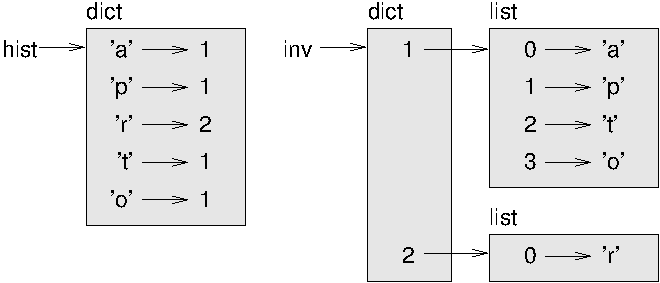
\includegraphics[scale = 0.8] {figs/dict1.pdf}}
\caption{Diagrama de Estado.}
\label{} fig.dict1
\end{figure}

Figura ~ \ref {} fig.dict1 é um diagrama mostrando estado {\tt hist} e {\tt inversa}.
Um dicionário é representado como uma caixa com o tipo {\tt dict} acima dele
e os pares de valores-chave dentro. Se os valores são inteiros, carros alegóricos ou
cordas, eu costumo chamar-lhes dentro da caixa, mas eu costumo chamar listas
fora da caixa, apenas para manter o simples diagrama.
\index{diagrama de estado}
\index{diagrama! Estado}

As listas podem ser valores em um dicionário, como mostra este exemplo, mas eles
não podem ser chaves. Veja o que acontece se você tentar:
\index{} TypeError
\index{exceção! TypeError}


\begin{verbatim}
>>> T = [1, 2, 3]
>>> D = dict ()
>>> D [t] = 'oops'
Traceback (most recent call last):
  Arquivo "<stdin>", linha 1, em?
TypeError: objetos da lista são unhashable
\end{verbatim}
%
Mencionei anteriormente que um dicionário é implementado usando
uma tabela hash, o que significa que as chaves têm que ser {\bf Hashable}.
\{Função hash} índice
\index{} Hashable

A {\bf de hash} é uma função que assume um valor (de qualquer tipo)
e retorna um inteiro. Dicionários usar estes números inteiros,
chamados valores de hash, para armazenar e procurar pares de valores-chave.
\index{imutabilidade}

Este sistema funciona bem se as chaves são imutáveis. Mas se o
chaves são mutáveis, como listas, coisas ruins acontecem. Por exemplo,
quando você cria um par chave-valor, Python hashes a chave e 
armazena no local correspondente. Se você modificar o
chave e, em seguida, hash-lo novamente, ele iria para um local diferente.
Nesse caso, você pode ter duas entradas para a mesma chave,
ou você pode não ser capaz de encontrar uma chave. De qualquer maneira, o
dicionário não iria funcionar corretamente.

É por isso que as chaves têm que ser Hashable, e por que tipos mutáveis, como
listas não são. A maneira mais simples de contornar essa limitação é
usar tuplas, que veremos no próximo capítulo.

Uma vez que os dicionários são mutáveis, eles não podem ser usadas como teclas,
mas eles {\em} pode ser usado como valores.

\begin{} exercício
Leia a documentação do método dicionário {\tt setdefault}
e usá-lo para escrever uma versão mais concisa do \verb "invert_dict".
Solução: \url{http://thinkpython.com/code/invert_dict.py}.
\{Método setdefault} índice
\index{método! Setdefault}

\end{} exercício


\section{} Memos

Se você jogou com o {\tt Fibonacci} function de
Seção ~ \ref {} one.more.example, você deve ter notado que a maior
o argumento que você fornecer, mais tempo a função demora para executar.
Além disso, o tempo de execução aumenta muito rapidamente.
\index{função Fibonacci}
\index{function! Fibonacci}

Para entender o porquê, considere a Figura ~ \ref {} fig.fibonacci, o que mostra
o gráfico {\bf chamada} para {\tt Fibonacci} com {\tt n = 4}:

\begin{figure}
\centerline
{\includegraphics[scale = 0.7] {figos / fibonacci.pdf}}
\caption{Gráfico de chamada.}
\label{} fig.fibonacci
\end{figure}

Um gráfico de chamadas mostra um conjunto de quadros de função, com linhas conectando cada
enquadrar aos quadros das funções que ele chama. Na parte superior do
gráfico, {\tt Fibonacci} com {\tt n = 4} chamadas {\tt Fibonacci} com {\tt
n = 3} e {\tt n = 2}. Por sua vez, {\tt Fibonacci} com {\tt n = 3} chamadas
{\tt Fibonacci} com {\tt n = 2} e {\tt n = 1}. E assim por diante.
\index{função frame}
\index{frame}
\{Gráfico de chamadas} índice

Conte quantas vezes {\tt Fibonacci (0)} e {\tt Fibonacci (1)} são
chamado. Esta é uma solução para o problema de ineficiente, e fica
pior que o argumento se torna maior.
\index{memo}

Uma solução é manter o controle de valores que já tenham sido
computadorizada, armazenando-os em um dicionário. Um valor previamente calculado
que é armazenado para uso posterior é chamado uma nota {\bf}. Aqui está um
implementação de {\tt Fibonacci} usando mensagens:

\begin{verbatim}
conhecido = {0:0, 1:01}

Fibonacci def (n):
    se n no conhecido:
        retornar conhecido [n]

    res = Fibonacci (n-1) + Fibonacci (n-2)
    conhecido [n] = res
    voltar res
\end{verbatim}
%
{\tt conhecido} é um dicionário que mantém o controle do Fibonacci
números que já conhecemos. Começa com
dois itens: 0 mapas a 0 e 1 a 1 mapas.

Sempre {\tt Fibonacci} é chamado, ele verifica {\tt conhecido}.
Se o resultado já está lá, ele pode retornar
imediatamente. Caso contrário, ele tem que
calcular o novo valor, adicioná-lo ao dicionário, e devolvê-lo.

\begin{} exercício

Executar esta versão do {\tt Fibonacci} eo original com
uma série de parâmetros e comparar os seus tempos de execução.

\end{} exercício

\begin{} exercício

Memoize a função de Ackermann do Exercício ~ \ref {} ackermann e ver se
memoization torna possível avaliar a função com maior
argumentos. Dica: não.
Solução: \url{http://thinkpython.com/code/ackermann_memo.py}.
\index{função de Ackermann}
\index{function! Ack}

\end{} exercício


\section{Variáveis ​​globais}
\index{variável global}
\index{variável! Mundial}

No exemplo anterior, {\tt conhecida} é criada do lado de fora da função,
por isso pertence ao quadro especial chamado \verb "__main__".
Variáveis ​​em \verb "__main__" às vezes são chamados {\bf mundial}
porque eles podem ser acessados ​​a partir de qualquer função. Ao contrário de locais
variáveis, que desaparecem quando a função termina, as variáveis ​​globais
persistir a partir de uma chamada de função para o próximo.
\index{flag}

É comum o uso de variáveis ​​globais para {flags \bf}, isto é, 
variáveis ​​booleanas que indicam (`` bandeira'') se uma condição
é verdadeiro. Por exemplo, alguns programas usam
uma bandeira chamada {\tt detalhado} para controlar o nível de detalhe no
saída:

\begin{verbatim}
verbose = True

example1 def ():
    se detalhado:
        imprimir 'example1 Running'
\end{verbatim}
%
Se você tentar transferir uma variável global, você pode ser surpreendido.
O exemplo a seguir é suposto para controlar se o
função foi chamado:
\index{atribuição múltipla}
\index{atribuição múltipla!}

\begin{verbatim}
been_called = False

example2 def ():
    been_called = True # ERRADO
\end{verbatim}
%
Mas se você executá-lo, você verá que o valor de \verb "been_called"
não muda. O problema é que {\tt example2} cria um novo local,
variável chamada \verb "been_called". A variável local desaparece quando
a função termina, e não tem efeito sobre a variável global.
\index{instrução global}
\index{declaração! Mundial}
\index{declaração}

Para voltar a atribuir uma variável global dentro de uma função que você tem que
{\bf} declare a variável global antes de usá-lo:

\begin{verbatim}
been_called = False

example2 def ():
    been_called mundial 
    been_called = True
\end{verbatim}
%
O {\tt mundial} declaração diz o intérprete
algo como `` Nesta função, quando eu digo \verb "been_called", eu
significa a variável global, não criar um local.''
\index{update! Variável global}
\index{variável global update!}

Aqui está um exemplo que tenta atualizar uma variável global:

\begin{verbatim}
contador = 0

Example3 def ():
    contador = contador + 1 # ERRADO
\end{verbatim}
%
Se você executá-lo você tem:
\index{} UnboundLocalError
\index{exceção! UnboundLocalError}

\begin{verbatim}
UnboundLocalError: variável local 'count' referenciado antes da atribuição
\end{verbatim}
%
Python assume que {\tt count} é local, o que significa
que você está lendo isso antes de escrevê-lo. A solução, de novo,
é declarar {count \tt} global.
\index{counter}

\begin{verbatim}
Example3 def ():
    contagem global
    contador + = 1
\end{verbatim}
%
Se o valor global é mutável, você pode modificá-lo sem
declarando-o:
\index{} mutabilidade

\begin{verbatim}
conhecido = {0:0, 1:01}

exemplo4 def ():
    conhecido [2] = 1
\end{verbatim}
%
Assim, você pode adicionar, remover e substituir os elementos de uma lista global ou
dicionário, mas se você deseja reatribuir a variável, você
tem que declarar que:

\begin{verbatim}
example5 def ():
    global conhecido
    conhecido = dict ()
\end{verbatim}
%

\section{inteiros longos}
\index{long integer}
\index{inteiro! Longo}
\index{type! Longo}

Se você calcular {\tt Fibonacci (50)}, você obtém:

\begin{verbatim}
>>> Fibonacci (50)
12586269025L
\end{verbatim}
%
O {\tt G} ao final indica que o resultado é um longo
inteiro, ou o tipo {\tt longo}. Em Python 3, {\tt longo} está desaparecido; todos os inteiros,
mesmo muito grandes, são do tipo {\tt int}.
\index{Python 3}

Valores com tipo {\tt int} têm um alcance limitado;
inteiros longos podem ser arbitrariamente grande, mas como eles ficam maiores
que consomem mais tempo e espaço.

Os operadores matemáticos trabalhar em inteiros longos, e as funções
no {\tt matemática} módulo, também, para que, em geral, qualquer código que
trabalha com {\tt int} também irá trabalhar com {\tt longo}.

Toda vez que o resultado de um cálculo é grande demais para ser representado com
um inteiro, Python converte o resultado como um inteiro longo:

\begin{verbatim}
>>> 1000 * 1000
1000000
>>> 100000 * 100000
10000000000L
\end{verbatim}
%
No primeiro caso, o resultado tem o tipo {\tt int}; no
segundo caso, é {\tt longo}.

\begin{} exercício
\index{} criptografia
\index{algoritmo RSA}
\index{algoritmo! RSA}

Exponenciação de grandes inteiros é a base de comum
algoritmos de criptografia de chave pública. Leia a Wikipedia
página sobre o algoritmo RSA (\url{http://en.wikipedia.org/wiki/RSA})
e escrever funções para codificar e decodificar mensagens.

TODO: solução para este!

\end{} exercício


\section{} Depuração
\index{depuração}

Enquanto você trabalha com conjuntos de dados maiores, pode se tornar inviável para
debug, imprimindo e verificando os dados à mão. Aqui estão alguns
sugestões para a depuração de grandes conjuntos de dados:

\begin{description}

\item[escala para baixo a entrada:] Se possível, reduzir o tamanho da
conjunto de dados. Por exemplo, se o programa lê um arquivo de texto, comece com
apenas as primeiras 10 linhas, ou com o menor exemplo, você pode encontrar.
Você pode editar os arquivos de si mesmos, ou (melhor) modificar o
programa para que ele lê apenas os primeiros {\tt n} linhas.

Se houver um erro, você pode reduzir {\tt n} para o menor
valor que se manifesta o erro e, em seguida, aumentá-la gradualmente
como você encontrar e corrigir erros.

\item[Verifique resumos e tipos:] Em vez de impressão e verificar o
conjunto de dados inteiro, considere imprimir os resumos dos dados: por exemplo,
o número de itens em um dicionário ou o total de uma lista de números.

Uma causa comum de erros de execução é um valor que não é o direito
digita. Para depurar esse tipo de erro, muitas vezes é o suficiente para impressão
o tipo de um valor.

\item[Escreva auto-verificações:] Às vezes, você pode escrever código para verificar
por erros automaticamente. Por exemplo, se você estiver calculando a
média de uma lista de números, você pode verificar que o resultado é
não é maior do que o maior elemento da lista ou menos de
a menor. Isso é chamado de `` verificação de sanidade'' porque ele detecta
resultados que são `` louco.''
\index{verificação de sanidade}
\index{verificação de consistência}

Um outro tipo de controlo compara os resultados de dois diferentes
cálculos para ver se eles são consistentes. Isto é chamado um
`` Verificação de consistência.''

\item[Bonito imprimir a saída:] Formatando saída de depuração
pode torná-lo mais fácil de detectar um erro. Vimos um exemplo na
Seção ~ \ref {} factdebug. O {\tt pprint} módulo fornece
uma {\tt pprint} função que exibe tipos embutidos em
um formato mais legível.
\index{muito print}
\index{módulo pprint}
\index{módulo! Pprint}

\end{description}

Mais uma vez, o tempo que você gasta andaimes de construção pode reduzir
o tempo que você gasta depuração.
\index{} andaimes

\section{} Glossário

\begin{description}

\item[dicionário]: Um mapeamento a partir de um conjunto de chaves para a sua
Os valores correspondentes.
\index{} dicionário

\item[par chave-valor:] A representação do mapeamento de
uma chave com um valor.
\index{par chave-valor}

\item[Item]: Outro nome para um par chave-valor.
\index{artigo! Dicionário}

\item[chave]: Um objeto que aparece em um dicionário como o
primeira parte de um par chave-valor.
\index{chave}

\item[valor]: Um objeto que aparece em um dicionário como o
segunda parte de um par chave-valor. Este é mais específico do que
nosso uso anterior da palavra `` valor.''
\index{value}

\item[aplicação]: A maneira de realizar um cálculo.
\index{implementação}

\item[hashtable:] O algoritmo usado para implementar Python
dicionários.
\index{} hashtable

\[Função hash:] item A função usada por uma tabela hash para calcular o
local para uma chave.
\{Função hash} índice

\item[Hashable:] Um tipo que tem uma função de hash. Imutável
tipos como inteiros,
bóias e cordas são Hashable; tipos mutáveis, como listas e
dicionários não são.
\index{} Hashable

\item[pesquisa]: Uma operação de dicionário que recebe uma chave e encontra
o valor correspondente.
\index{pesquisa}

\item[pesquisa inversa:] Uma operação de dicionário que assume um valor e encontra
uma ou mais chaves que mapeiam a ele.
\index{pesquisa inversa, dicionário}

\item[singleton:] A lista (ou outra seqüência) com um único elemento.
\index{singleton}

\item[chamar gráfico:] Um diagrama que mostra cada quadro criado durante
a execução de um programa, com uma flecha de cada chamador
cada receptor. 
\{Gráfico de chamadas} índice
\index{diagrama gráfico chamada!}

\item[histograma:] Um conjunto de contadores.
\index{} histograma

\item[memorando:] Um valor calculado armazenado para evitar futuras desnecessário 
computação.
\index{memo}

\item[variável global:] Uma variável definida fora de uma função. Global
variáveis ​​podem ser acessados ​​a partir de qualquer função.
\index{variável global}

\item[flag]: A variável booleana usada para indicar se uma condição
é verdadeiro.
\index{flag}

\item[declaração]: Uma declaração como {\tt mundial} que conta a
intérprete algo sobre uma variável.
\index{declaração}

\end{description}

\section{Exercícios}

\begin{} exercício
\index{} duplicado

Se você fez o exercício ~ \ref {} duplicado, você já tem
uma função chamada \verb "has_duplicates" que recebe uma lista
como um parâmetro e retorna {\tt true} se houver qualquer objeto
que aparece mais do que uma vez na lista.

Use um dicionário para escrever uma versão mais rápida, mais simples de
\verb "has_duplicates". 
Solução: \url{http://thinkpython.com/code/has_duplicates.py}.

\end{} exercício


\begin{} exercício
\label{} exrotatepairs
\index{rotação letter}
\index{rotação! Letras}

Duas palavras são `` pares rotação'' se você pode girar uma delas
e obter o outro (ver \verb "rotate_word" no Exercício ~ \ref {exrotate}).

Escreva um programa que lê uma lista de palavras e encontra toda a rotação
pares. Solução: \url{http://thinkpython.com/code/rotate_pairs.py}.

\end{} exercício


\begin{} exercício
\index{Car Talk}
\index{} Puzzler

Aqui está outra Puzzler de {Car \em
Fale} (\url{http://www.cartalk.com/content/puzzlers}):

\begin{quote}
Este foi enviado por um sujeito chamado Dan O'Leary. Ele chegou a um comum
uma sílaba, palavra de cinco letras, recentemente, que tem o seguinte único
propriedade. Quando você remove a primeira letra, as cartas restantes formam
um homófono da palavra original, que é uma palavra que soa exatamente
o mesmo. Substitua a primeira letra, ou seja, colocá-lo de volta e retire
a segunda letra eo resultado é mais um homófono do
palavra original. E a pergunta é, qual é a palavra?

Agora eu estou indo dar-lhe um exemplo que não funciona. Vejamos
a palavra de cinco letras: 'destroços'. WRACK, você sabe que gosto de `naufragar com
dor. ' Se eu remover a primeira carta, eu fiquei com uma carta de quatro
palavra, 'RACK. Como em `Caramba, você viu o rack em que fanfarrão!
Deve ter sido um ponteiro nove! " É uma homofonia perfeito. Se você
colocar o `w 'de volta, e remover o` r', em vez disso, você fica com o
palavra, 'bosta', que é uma palavra real, que não é apenas um homófono do
outras duas palavras.

Mas há, no entanto, pelo menos uma palavra que Dan e nós sabemos de,
que irá produzir dois homophones se você remover um dos dois primeiros
cartas para fazer duas, novas palavras de quatro letras. A questão é, o que é
a palavra?
\end{quote}
\index{} homófono
\index{palavra redutível}
\index{palavra, redutível}

Você pode usar o dicionário do Exercício ~ \ref {} wordlist2 para verificar
se uma string está na lista de palavras.

Para verificar se duas palavras são palavras homófonas, você pode usar o CMU
Pronunciar Dictionary. Você pode baixá-lo a partir de
\url{http://www.speech.cs.cmu.edu/cgi-bin/cmudict} ou a partir de
\url{http://thinkpython.com/code/c06d} e você também pode fazer download
\url{http://thinkpython.com/code/pronounce.py}, que fornece uma função
chamado \verb "read_dictionary" que lê o dicionário e pronúncia
retorna um dicionário Python que mapeia a partir de cada palavra como uma seqüência que
descreve a sua principal pronúncia.

Escreva um programa que lista todas as palavras que resolvem o Puzzler.
Solução: \url{http://thinkpython.com/code/homophone.py}.

\end{} exercício



\chapter{} Tuples
\label{} tuplechap

\section{Tuplas são imutáveis}
\index{} tupla
\index{type! Tupla}
\index{seqüência}

Uma tupla é uma seqüência de valores. Os valores podem ser de qualquer tipo, e
eles são indexados por inteiros, portanto, em que o respeito tuplas são muito
como listas. A diferença importante é que as tuplas são imutáveis.
\index{} mutabilidade
\index{imutabilidade}

Sintaticamente, uma tupla é uma lista de valores separados por vírgulas:

\begin{verbatim}
>>> T = 'a', 'b', 'c', 'd', 'e'
\end{verbatim}
%
Embora não seja necessário, é comum incluir tuplas
parênteses:
\index {parênteses! tuplas em}

\begin{verbatim}
>>> T = ('a', 'b', 'c', 'd', 'e')
\end{verbatim}
%
Para criar uma tupla com um único elemento, você tem que incluir uma final
vírgula:
\index{singleton}
\index{tupla! Singleton}

\begin{verbatim}
>>> T1 = 'a',
>>> Type (t1)
<type'tuple'>
\end{verbatim}
%
Um valor entre parênteses não é uma tupla:

\begin{verbatim}
>>> T2 = ('A')
>>> Type (t2)
<type'str'>
\end{verbatim}
%
Outra maneira de criar uma tupla é a função built-in {\tt tupla}.
Sem argumento, ele cria uma tupla vazia:
\index{função tupla}
\index{function! Tupla}

\begin{verbatim}
>>> T = tuple ()
>>> Print t
()
\end{verbatim}
%
Se o argumento é uma seqüência (string, lista ou tupla), o resultado
é um tuplo com os elementos da sequência:

\begin{verbatim}
>>> T = tupla ('tremoços')
>>> Print t
('L', 'u', 'p', 'i', 'n', 's')
\end{verbatim}
%
Porque {\tt tupla} é o nome de uma função built-in, você deve
evite usá-lo como um nome de variável.

A maioria dos operadores de lista também trabalhar em tuplas. O operador colchete
índices de um elemento:
\index{operador colchete}
\index{operador! Suporte}

\begin{verbatim}
>>> T = ('a', 'b', 'c', 'd', 'e')
>>> Print t [0]
'A'
\end{verbatim}
%
E o operador de fatia seleciona um intervalo de elementos.
\index{operador de fatia}
\index{operador! Fatia}
\index{tupla! Fatia}
\index{fatia! Tupla}

\begin{verbatim}
>>> Print t [01:03]
('B', 'c')
\end{verbatim}
%
Mas se você tentar modificar um dos elementos da tupla, você começa
um erro:
\index{exceção! TypeError}
\index{} TypeError
\{} Atribuição item de índice
\index{atribuição! Artigo}

\begin{verbatim}
>>> T [0] = 'A'
TypeError: objeto não suporta atribuição artigo
\end{verbatim}
%
Você não pode modificar os elementos de uma tupla, mas você pode substituir
uma tupla com outro:

\begin{verbatim}
>>> T = ('A',) + t [1:]
>>> Print t
('A', 'b', 'c', 'd', 'e')
\end{verbatim}
%

\section{atribuição Tuple}
\label{} tuple.assignment
\index{tupla! Atribuição}
\index{atribuição! Tupla}
\index{padrão de swap}
\index{padrão! Troca}

Muitas vezes, é útil para trocar os valores de duas variáveis.
Com atribuições convencionais, você tem que usar um temporário
variável. Por exemplo, para trocar {\tt a} e {\tt b}:

\begin{verbatim}
Temp = >>> um
>>> A = b
>>> B = temperatura
\end{verbatim}
%
Esta solução é pesado; {\bf atribuição de tupla} é mais elegante:

\begin{verbatim}
>>> A, b = b, um
\end{verbatim}
%
A ala esquerda é uma tupla de variáveis, o lado direito é uma tupla de
expressões. Cada valor é atribuída a sua respectiva variável.  
Todas as expressões do lado direito são avaliadas antes de qualquer
das atribuições.

O número de variáveis ​​do lado esquerdo e do número de
Os valores da direita tem que ser a mesma:
\index{exceção! ValueError}
\index{} ValueError

\begin{verbatim}
>>> A, b = 1, 2, 3
ValueError: muitos valores para desempacotar
\end{verbatim}
%
Mais geralmente, o lado direito pode ser de qualquer tipo de sequência
(String, lista ou tupla). Por exemplo, para dividir um endereço de e-mail
em um nome de usuário e um domínio, você poderia escrever:
\{Método split} índice
\index{método! Divisão}
\index{email}

\begin{verbatim}
>>> Addr = 'monty@python.org'
>>> Uname, domain = addr.split ("@")
\end{verbatim}
%
O valor de retorno {\tt divisão} é uma lista com dois elementos;
o primeiro elemento é atribuído a {\tt uname}, segundo a
{Domain tt \}.

\begin{verbatim}
>>> Print uname
monty
>>> Domínio impressão
python.org
\end{verbatim}
%

\section{Tuplas como valores de retorno}
\index{} tupla
\index{value! Tupla}
\index{valor de retorno! Tupla}
\index{função, tupla como valor de retorno}

Estritamente falando, a função só pode retornar um valor, mas
se o valor for um tuplo, o efeito é o mesmo que o retorno
vários valores. Por exemplo, se você quer dividir dois números inteiros
e calcular o quociente eo resto, é ineficiente para
calcular {\tt x / y} e depois {\tt x \y}. É preferível calcular
os dois ao mesmo tempo.
\index{} divmod

A função built-in {\tt divmod} tem dois argumentos e
retorna uma tupla de dois valores, o quociente eo resto.
Você pode armazenar o resultado como uma tupla:

\begin{verbatim}
>>> T = divmod (7, 3)
>>> Print t
(2, 1)
\end{verbatim}
%
Ou use atribuição de tupla para armazenar os elementos separadamente:
\index{atribuição de tupla}
\index{atribuição! Tupla}

\begin{verbatim}
>>> Quot, rem = divmod (7, 3)
>>> Print quot
2
>>> Print rem
1
\end{verbatim}
%
Aqui está um exemplo de uma função que retorna uma tupla:

\begin{verbatim}
min_max def (t):
    retornar min (t), max (t)
\end{verbatim}
%
{\tt max} e {\tt min} são built-in funções que encontram
os elementos maiores e menores de uma seqüência. \Verb "min_max"
calcula tanto e retorna uma tupla de dois valores.
\{Função max} índice
\index{function! Max}
\index{min função}
\index{function! Min}


\section{argumentos de comprimento variável tuplas}
\index{de comprimento variável argumento tupla}
\index{argumento! De comprimento variável tupla}
\index{reunir}
\index{parâmetro! Reunir}
\index{argumento! Reunir}

As funções podem ter um número variável de argumentos. Um parâmetro
nome que começa com {\tt *} {recolhe \bf} argumentos em
uma tupla. Por exemplo, {\tt printall}
toma qualquer número de argumentos e imprime-los:

\begin{verbatim}
def printall (* args):
    args impressão
\end{verbatim}
%
O parâmetro de recolher pode ter qualquer nome que quiser, mas {args \tt} é
convencional. Veja como a função funciona:

\begin{verbatim}
>>> Printall (1, 2,0, '3 ')
(1, 2,0, '3 ')
\end{verbatim}
%
O complemento de recolher é {\bf dispersão}. Se você tem um
seqüência de valores e quer passá-lo para uma função
como vários argumentos, você pode usar o {\tt *} operador.
Por exemplo, {\tt divmod} tem exatamente dois argumentos, que
não funciona com uma tupla:

Removendo isso, porque nós não vimos ainda os parâmetros opcionais
Você pode combinar o operador se reunir com exigido e posicional
argumentos:

%\begin{verbatim}
Def inúteis (obrigatório, opcional = 0, * args):
De impressão obrigatória, opcional args
\end{verbatim}
\afterverb
%
Execute esta função com 1, 2, 3 e 4 ou mais argumentos e
Certificar que você entendeu o que ele faz.
\index{dispersão}
\index{argumento dispersão}
\index{} TypeError
\index{exceção! TypeError}

\begin{verbatim}
>>> T = (7, 3)
>>> Divmod (t)
TypeError: divmod esperado 2 argumentos, tem um
\end{verbatim}
%
Mas se você espalhar a tupla, ele funciona:

\begin{verbatim}
>>> Divmod (* t)
(2, 1)
\end{verbatim}
%
\begin{} exercício

Muitas das funções internas usar
argumentos de comprimento variável tuplas. Por exemplo, {\tt max}
e {\tt min} pode ter qualquer número de argumentos:
\{Função max} índice
\index{function! Max}
\index{min função}
\index{function! Min}

\begin{verbatim}
>>> Max (1,2,3)
3
\end{verbatim}
%
Mas {soma \tt} não.
\{} Função soma índice
\index{function! Soma}

\begin{verbatim}
>>> Soma (1,2,3)
TypeError: soma esperada na maioria dos 2 argumentos, tenho 3
\end{verbatim}
%
Escreva uma função chamada {\tt sumall} que aceita qualquer número
de argumentos e retorna a soma deles.

\end{} exercício


\section{listas e tuplas}
\{Função zip} índice
\index{function! Zip}

{\tt zip} é uma função built-in que leva dois ou mais seqüências e
``'' Fecha-los em uma lista de tuplas, onde cada tupla contém um
elemento de cada sequência. Em Python 3, {\tt zip} retorna um iterador
de tuplas, mas na maioria dos casos, um iterador se comporta como uma lista.
\index{Python 3}

Este exemplo fecha uma corda e uma lista:

\begin{verbatim}
>>> S = 'abc'
>>> T = [0, 1, 2]
>>> Zip (s, t)
[('A', 0), ('b', 1), ('c', 2)]
\end{verbatim}
%
O resultado é uma lista de tuplas, onde cada tupla contém
um personagem da corda eo elemento correspondente de
lista.
\index{list! De tuplas}

Se as sequências não têm o mesmo comprimento, o resultado tem o
comprimento do mais curto.

\begin{verbatim}
>>> Zip ('Anne', 'Elk')
[('A', 'E'), ('n', 'l'), ('n', 'k')]
\end{verbatim}
%
Você pode usar atribuição de tupla em uma {\tt for} loop para percorrer uma lista de
tuplas:
\index{travessia}
\index{atribuição de tupla}
\index{atribuição! Tupla}

\begin{verbatim}
t = [('a', 0), ('b', 1), ('c', 2)]
por letra, número de t:
    número de impressão, carta
\end{verbatim}
%
Cada vez através do loop, Python seleciona a próxima tupla em
a lista e atribui os elementos para {\tt carta} e 
{Número tt \}. A saída deste circuito é a seguinte:
\index{laço}

\begin{verbatim}
0 um
1-B
2 c
\end{verbatim}
%
Se você combinar {\tt zip}, {\tt for} e atribuição de tupla, você recebe um
expressão útil para a travessia de dois (ou mais) as sequências na mesma
tempo. Por exemplo, \verb "has_match" leva duas sequências, {\tt t1} e
{\tt t2}, e retorna {\tt true} se houver um índice {\tt i}
tal que {\tt t1 [i] == t2 [i]}:
\index{loop}

\begin{verbatim}
has_match def (T1, T2):
    para x, y em zip (T1, T2):
        if x == y:
            retornar True
    retornará False
\end{verbatim}
%
Se você precisa atravessar os elementos de uma seqüência e sua
índices, você pode usar a função built-in {\tt enumerate}:
\index{travessia}
\index{enumerar função}
\index{função enumerate!}

\begin{verbatim}
para o índice, elemento em enumerar ('abc'):
    de impressão de índice, elemento
\end{verbatim}
%
A saída deste circuito é a seguinte:

\begin{verbatim}
0 um
1-B
2 c
\end{verbatim}
%
Mais uma vez.


\section{Dicionários e tuplas}
\label{} dictuple
\index{} dicionário
\index{itens método}
\index{método! Itens}
\index{par chave-valor}

Dicionários ter um método chamado {itens \tt} que retorna uma lista de
tuplas, onde cada tupla é um par chave-valor.

\begin{verbatim}
>>> D = {'a': 0, 'b': 1, 'c': 2}
>>> T = d.items ()
>>> Print t
[('A', 0), ('c', 2), ('b', 1)]
\end{verbatim}
%
Como você deve esperar de um dicionário, os itens não são de
ordem particular. Em Python 3, {items \tt} retorna um iterador,
mas para muitos propósitos, iteradores se comportam como listas.

Indo em outra direção, você pode usar uma lista de tuplas de
inicializar um novo dicionário: \index {! dicionário inicializar}

\begin{verbatim}
>>> T = [('a', 0), ('c', 2), ('b', 1)]
>>> D = dict (t)
>>> Print d
{'A': 0, 'c': 2, 'b': 1}
\end{verbatim}

Combinando {\tt dict} com {\tt zip} produz uma forma concisa
para criar um dicionário:
\index{função zip! Usar com dict}

\begin{verbatim}
>>> D = dict (zip ('abc', range (3)))
>>> Print d
{'A': 0, 'c': 2, 'b': 1}
\end{verbatim}
%
O método de dicionário {update \tt} também tem uma lista de tuplas
e adiciona-los, como pares de valores-chave, para um dicionário existente.
\index{método update}
\index{método! Update}
\index{atravessar! Dicionário}
\index{dicionário! Travessia}

Combinando itens {\tt}, atribuição de tupla e {\tt para}, você
obter o idioma para atravessar as chaves e valores de um dicionário:

\begin{verbatim}
para a chave, val em d.items ():
    impressão val, key
\end{verbatim}
%
A saída deste circuito é a seguinte:

\begin{verbatim}
0 um
2 c
1-B
\end{verbatim}
%
Mais uma vez.

É comum o uso de tuplas como chaves em dicionários (principalmente porque
você não pode usar as listas). Por exemplo, uma lista telefônica pode mapear
do último nome, pares primeiro nome para números de telefone. Assumindo
que definimos {\tt última}, {\tt primeiro} e {número \tt}, nós
poderia escrever:
\index{tupla! Como chave no dicionário}
\index{} Hashable

\begin{verbatim}
diretório [passado, primeiro] = número
\end{verbatim}
%
A expressão entre parênteses é uma tupla. Nós poderíamos usar tupla
atribuição para atravessar este dicionário.
\index{tupla! Entre colchetes}

\begin{verbatim}
para o último, primeiro no diretório:
    imprimir primeiro, último, diretório [passado, primeiro]
\end{verbatim}
%
Este loop percorre as chaves {diretório \tt}, que são tuplas. Ele
atribui os elementos de cada tupla para {\tt última} e {\tt primeiro}, então
imprime o nome eo número de telefone correspondente.

Há duas maneiras de representar tuplas em um diagrama de estado. O mais
versão detalhada mostra os índices e elementos da mesma forma que aparecem na
uma lista. Por exemplo, a tupla \verb "('Cleese', 'John')" parece
como na Figura ~ \ref {fig.tuple1}.
\index{diagrama de estado}
\index{diagrama! Estado}

\begin{figure}
\centerline
{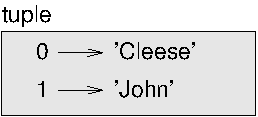
\includegraphics[scale = 0.8] {figs/tuple1.pdf}}
\caption{Diagrama de Estado.}
\label{} fig.tuple1
\end{figure}

Mas, em um diagrama maior você pode querer deixar de fora a
detalhes. Por exemplo, um diagrama da lista telefônica pode
aparecer como na Figura ~ \ref {} fig.dict2.

\begin{figure}
\centerline
{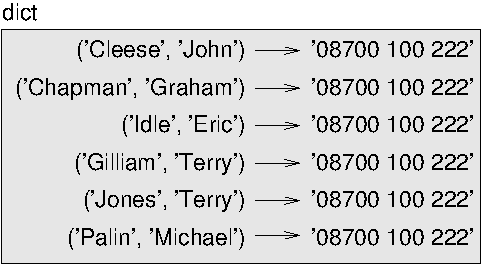
\includegraphics[scale = 0.8] {figs/dict2.pdf}}
\caption{Diagrama de Estado.}
\label{} fig.dict2
\end{figure}

Aqui as tuplas são mostrados usando a sintaxe do Python como uma gráfica
taquigrafia.

O número de telefone no diagrama é a linha de queixas para o
BBC, por isso, não chamá-lo.



\section{} Comparando tuplas
\index{comparação! Tupla}
\index{tupla Comparação}
\{} Método de classificação do índice
\index{método! Tipo}

Os operadores relacionais trabalhar com tuplas e outras sequências;
Pitão começa por comparar o primeiro elemento de cada
seqüência. Se eles forem iguais, ele vai para as próximas elementos,
e assim por diante, até que encontre elementos que diferem. Subseqüente
elementos não são considerados (mesmo se eles são realmente grandes).

\begin{verbatim}
>>> (0, 1, 2) <(0, 3, 4)
Verdadeiro
>>> (0, 1, 2000000) <(0, 3, 4)
Verdadeiro
\end{verbatim}
%
O {\tt tipo} function funciona da mesma maneira. Ele classifica
principalmente pelo primeiro elemento, mas no caso de um laço, que classifica
pelo segundo elemento, e assim por diante.  

Este recurso se presta a um padrão chamado {\bf DSU} para 

\begin{description}

\item[Decore] uma seqüência através da construção de uma lista de tuplas
com uma ou mais chaves de classificação anteriores os elementos da seqüência,

\item[Ordem] a lista de tuplas, e

\item[undecorate], extraindo os elementos ordenados da seqüência.

\end{description}

\label{} DSU
\index{padrão DSU}
\index{padrão! DSU}
\index{decorar-sort-undecorate padrão}
\index{padrão! Decorar-sort-undecorate}

Por exemplo, suponha que você tenha uma lista de palavras e você quer
classificá-los de maior para o menor:

\begin{verbatim}
def sort_by_length (palavras):
    t = []
    por palavra nas palavras:
       t.append ((len (palavra), palavra))

    t.sort (reverse = True)

    res = []
    por comprimento, palavra em t:
        res.append (palavra)
    voltar res
\end{verbatim}
%
O primeiro loop cria uma lista de tuplas, onde cada
tupla é uma palavra precedida por seu comprimento.

{\tt espécie} compara o primeiro elemento, o comprimento, por um lado, e
considera apenas o segundo elemento para desempatar. O argumento palavra-chave
{\tt reverter = True} diz {\tt tipo} para ir em ordem decrescente.
\index{argumento palavra-chave}
\index{argumento! Keyword}
\index{travessia}

O segundo loop percorre a lista de tuplas e cria uma lista de
palavras em ordem de comprimento decrescente.

\begin{} exercício

Neste exemplo, os laços são quebrados, comparando palavras, então palavras
com o mesmo comprimento aparecem em ordem alfabética inversa. Por outro
aplicativos que você pode querer quebrar os laços de forma aleatória. Modificar
neste exemplo, de modo que as palavras com o mesmo comprimento de aparecer na
ordem aleatória. Dica: veja a função {\tt random} no
{Random \tt} módulo.
Solução: \url{http://thinkpython.com/code/unstable_sort.py}.

\index{módulo random}
\index{módulo! Random}
\index{função random}
\index{function! Random}

\end{} exercício


\section{seqüências de seqüências}
\index{seqüência}

Tenho focado em listas de tuplas, mas quase todos os exemplos em
Neste capítulo também trabalha com listas de listas, tuplas de tuplas e
tuplas de listas. Para evitar enumerar as combinações possíveis, ele
Às vezes é mais fácil falar sobre seqüências de seqüências.

Em muitos contextos, os diferentes tipos de seqüências (strings, listas e
tuplas) podem ser usados ​​alternadamente. Então, como e por que você escolha uma
sobre os outros?
\index{string}
\index{lista}
\index{} tupla
\index{} mutabilidade
\index{imutabilidade}

Para começar com o óbvio, cordas são mais limitados do que os outros
seqüências porque os elementos têm de ser personagens. Eles são
também imutável. Se você precisa a capacidade de mudar os personagens
em uma string (em vez de criar uma nova string), você pode
quer usar uma lista de caracteres em seu lugar.

As listas são mais comuns do que as tuplas, principalmente porque eles são mutáveis.
Mas há alguns casos em que você pode preferir tuplas:

\begin{enumerate}

\item Em alguns contextos, como uma {return \tt} declaração, é
sintaticamente mais simples para criar uma tupla de uma lista. Em outra
contextos, talvez você prefira uma lista.

\item Se você quiser usar uma seqüência como uma chave de dicionário,
tem que usar um tipo imutável como uma tupla ou string.

\item Se você está passando por uma seqüência como um argumento para uma função,
usando tuplas reduz o potencial de um comportamento inesperado
devido a aliasing.

\end{enumerate}

Porque tuplas são imutáveis, eles não fornecem métodos
como {\tt tipo} e {\tt inversa}, que modificar listas existentes.
Mas Python fornece as funções built-in {\tt classificadas}
e {\tt revertida}, que levam qualquer seqüência como parâmetro
e retornar uma nova lista com os mesmos elementos em uma diferente
ordem.
\index{função ordenados}
\index{function! Classificadas}
\index{função invertida}
\index{function! Revertida}


\section{} Depuração
\index{depuração}
\index{estrutura de dados}
\index{error forma}
\index{erro! Forma}

Listas, dicionários e tuplas são conhecidos genericamente como {data \bf
  estruturas}; neste capítulo estamos começando a ver os dados compostos
estruturas, tais como listas de tuplas e dicionários que contêm tuplas
como chaves e listas como valores. Estruturas de dados compostos são úteis, mas
eles são propensos a que eu chamo {forma \bf erros}, isto é, os erros
causada quando uma estrutura de dados tem o tipo errado, tamanho ou composição.
Por exemplo, se você está esperando uma lista com um número inteiro e eu
dar-lhe um número inteiro e velho (e não em uma lista), não vai funcionar.
\index{módulo structshape}
\index{módulo! Structshape}

TODO: structshape agora faz parte do Swampy

Para ajudar a depurar esses tipos de erros, eu escrevi um módulo
chamado {\tt structshape} que fornece uma função, também chamada
{\tt structshape}, que leva a qualquer tipo de estrutura de dados como
um argumento e retorna um string que resume a sua forma.
Você pode baixá-lo a partir de \url{http://thinkpython.com/code/structshape.py}

Aqui está o resultado de uma simples lista:

\begin{verbatim}
>>> From structshape importação structshape
>>> T = [1,2,3]
>>> Print structshape (t)
lista de 3 int
\end{verbatim}
%
Um programa mais sofisticado poderia escrever `` lista de 3 int {\em s}'', mas
Era mais fácil não lidar com plurais. Aqui está uma lista de listas:

\begin{verbatim}
>>> T2 = [[1,2], [3,4], [5,6]]
>>> Print structshape (t2)
lista de 3 Lista de 2 int
\end{verbatim}
%
Se os elementos da lista não são do mesmo tipo,
{\tt structshape} agrupa, em ordem, por tipo:

\begin{verbatim}
>>> T3 = [1, 2, 3, 4,0, 5 ", 6", [7], [8], 9]
>>> Print structshape (t3)
lista de (3 int, float, 2 tempos, 2 lista de int, int)
\end{verbatim}
%
Aqui está uma lista de tuplas:

\begin{verbatim}
>>> S = 'abc'
>>> Lt = zip (t, s)
>>> Print structshape (lt)
lista de 3 tuplas (int, str)
\end{verbatim}
%
E aqui está um dicionário com 3 itens que mapeiam inteiros para strings.

\begin{verbatim}
>>> D = dict (lt) 
>>> Structshape impressão (d)
dict de 3 int-> str
\end{verbatim}
%
Se você está tendo problemas para manter o controle de suas estruturas de dados,
{\tt structshape} pode ajudar.


\section{} Glossário

\begin{description}

\item[tupla:] Uma seqüência imutável de elementos.
\index{} tupla

\item[tupla atribuição:] A cessão com uma sequência no
lado direito e uma tupla de variáveis ​​do lado esquerdo. O direito
lado é avaliado e, em seguida, os seus elementos são designados para o
variáveis ​​sobre a esquerda.
\index{atribuição de tupla}
\index{atribuição! Tupla}

\item[reunir]: A operação de montagem de um de comprimento variável
argumento tupla.
\index{reunir}

\item[dispersão:] A operação de tratamento de uma seqüência como uma lista de
argumentos.
\index{dispersão}

\item[DSU:] Abreviatura de `` decorar-sort-undecorate,'' um
padrão que envolve a construção de uma lista de tuplas, classificação e
extração de parte do resultado.
\index{padrão DSU}

\item[estrutura de dados:] Uma coleção de valores relacionados, muitas vezes
organizada em listas, dicionários, tuplas, etc
\index{estrutura de dados}

\item[forma (de uma estrutura de dados):] Um resumo do tipo,
tamanho e composição de uma estrutura de dados.
\index{} forma

\end{description}


\section{Exercícios}

\begin{} exercício

Escreva uma função chamada \verb "most_frequent" que recebe uma string e
imprime as letras em ordem decrescente de freqüência. Localizar texto
amostras de vários idiomas diferentes e ver como carta de frequência
varia entre as línguas. Compare seus resultados com as tabelas em
\url{http://en.wikipedia.org/wiki/Letter_frequencies}. Solução:
\url{http://thinkpython.com/code/most_frequent.py}. \index{letra
  freqüência} \index {! carta freqüência}

\end{} exercício


\begin{} exercício
\label{} anagramas
\index{set anagrama}
\index{set! Anagrama}

Mais anagramas!

\begin{enumerate}

\item Escreva um programa
que lê uma lista de palavras de um arquivo (veja Seção ~ \ref {lista de palavras}) e
imprime todos os conjuntos de palavras que são anagramas.

Aqui está um exemplo do que a saída poderia ser assim:

\begin{verbatim}
['Deltas', 'dessalinizar', 'durou', 'salgado', 'programado', 'staled']
['retentores', 'ternários']
['Geração', 'greatening']
['resmelts', 'fundições', 'sem fim']
\end{verbatim}
%
Dica: você pode querer construir um dicionário que mapeia a partir de um
conjunto de cartas para uma lista de palavras que pode ser escrito com os
letras. A pergunta é, como você pode representar o conjunto de
cartas de uma forma que pode ser usado como uma chave de?

\item Modifique o programa anterior para que ele imprime o maior conjunto
de anagramas primeiro, seguido por um segundo conjunto maior, e assim por diante.
\index{} Scrabble
\index{} bingo

\item Em Scrabble um `` bingo'' é quando você joga todas as sete peças em
seu rack, juntamente com uma carta no tabuleiro, de modo a formar um oito letras
palavra. O conjunto de 8 letras forma o máximo possível de bingos?
Dica: há sete anos.

(7, ['o mais irritado', 'adstringir', 'ganister', 'pórtico', 'granitos',
'ingratos', 'rangiest'])

Solução: \url{http://thinkpython.com/code/anagram_sets.py}.

\end{enumerate}
\end{} exercício

\begin{} exercício
\index{} metátese

Duas palavras formar um `` par metátese'' se você pode transformar um no
outro, trocando duas letras, por exemplo, `` conversar'' e
`` Conserva.'' Escreva um programa que encontra todos os pares de metátese
no dicionário. Dica: não testar todos os pares de palavras, e não fazer
testar todos os swaps possíveis. Solução: \url{http://thinkpython.com/code/metathesis.py}.
Crédito: Este exercício foi inspirado em um exemplo em \url{http://puzzlers.org}.

\end{} exercício



\begin{} exercício
\index{Car Talk}
\index{} Puzzler

Aqui está mais uma conversa sobre carros Puzzler
(\url{http://www.cartalk.com/content/puzzlers}):

\begin{quote}
Qual é a palavra mais longa Inglês, que continua a ser uma palavra em Inglês válido,
como você remover suas cartas, uma de cada vez?

Agora, as letras podem ser removidas a partir de uma das extremidades, ou no meio, mas
não pode reorganizar qualquer das cartas. Toda vez que você solta uma carta, você
acabar com outra palavra em Inglês. Se você fizer isso, você está finalmente
vai acabar com uma letra e que também vai ser uma
Inglês palavra --- um que é encontrada no dicionário. Eu quero saber
qual é a palavra mais longa e quantas letras faz
tem?

Vou dar-lhe um pequeno exemplo modesto: Sprite. Ok? Você começa
fora com sprite, você toma uma letra fora, um do interior do
palavra, pegue a r distância, e ficamos com a palavra despeito, então nós
tomar o e fora da final, ficamos com espeto, tomamos as s off, estamos
deixou com poço, ele e I.
\end{quote}
\index{palavra redutível}
\index{palavra, redutível}

Escreva um programa para encontrar todas as palavras que podem ser reduzidos, desta forma,
e, em seguida, encontrar a mais longa.

Este exercício é um pouco mais desafiador do que a maioria, por isso aqui estão
algumas sugestões:

\begin{enumerate}

\item Você pode querer escrever uma função que recebe uma palavra e
  calcula uma lista de todas as palavras que podem ser formadas através da remoção de um
  carta. Estas são as crianças ``'' da palavra.
\index{definição recursiva}
\index{definição! Recursiva}

\item Recursively, uma palavra é redutível se algum de seus filhos
são redutíveis. Como um caso base, você pode considerar o vazio
corda redutível.

\item A lista de palavras que eu forneci, {\tt words.txt}, não
conter simples palavras da letra. Assim, você pode querer adicionar
`` I'', `` a'', e uma string vazia.

\item Para melhorar o desempenho do seu programa, você pode querer
para memoize as palavras que são conhecidas por serem redutíveis.

\end{enumerate}

Solução: \url{http://thinkpython.com/code/reducible.py}.

\end{} exercício




\begin{} exercício
\url{http://en.wikipedia.org/wiki/Word_Ladder}
\end{} exercício




\chapter{Estudo de caso: seleção de estrutura de dados}

\section{análise de freqüência Palavra}
\label{análise}

Como de costume, você deve pelo menos tentar os seguintes exercícios
antes de ler as minhas soluções.

\begin{} exercício

Escreva um programa que lê um arquivo, divide cada linha em
palavras, retira os espaços em branco e pontuação das palavras, e
converte-os em minúsculas.
\index{módulo string}
\index{módulo! String}

Dica: A {string \tt} módulo fornece seqüências nomeadas {\tt espaço em branco},
que contém o espaço, tabulação, nova linha, etc, e {\tt
  pontuação} que contém os caracteres de pontuação. Vamos ver
se podemos fazer Python juro:

\begin{verbatim}
>>> Import string
>>> Print string.punctuation
!.? "# $& '() * +, - /:; <=> @ [\] ^ _` {|} ~
\end{verbatim}
%
Além disso, você pode considerar o uso dos métodos de string {tira \tt},
{\tt substituir} e {\tt traduzir}.
\{Método strip} índice
\index{método! Strip}
\index{método substituir}
\index{método! Substituir}
\index{método traduzir}
\index{método! Traduzir}

\end{} exercício


\begin{} exercício
\index{Projeto Gutenberg}

Vá para Project Gutenberg (\url{gutenberg.org}) e fazer o download 
o seu favorito livro fora de copyright em formato de texto simples.
\index{text plain}
\index{text! Plain}

Modifique o programa do exercício anterior para ler o livro
você baixou, pular sobre as informações de cabeçalho no início
do arquivo, e processar o resto das palavras como antes.

Em seguida, modifique o programa para contar o número total de palavras em
o livro, bem como o número de vezes que cada palavra é usada.
\index{freqüência de palavras}
\{! Palavra freqüência} índice

Imprimir o número de palavras diferentes usados ​​no livro. Comparar
diferentes livros de diferentes autores, escritos em épocas diferentes.
Que autor utiliza o mais extenso vocabulário?
\end{} exercício


\begin{} exercício

Modifique o programa do exercício anterior para imprimir o
20 palavras usadas com mais frequência no livro.

\end{} exercício


\begin{} exercício

Modifique o programa anterior para ler uma lista de palavras (ver
Seção ~ \ref {lista de palavras}) e, em seguida, imprimir todas as palavras do livro que
não estão na lista de palavras. Como muitos deles são erros de digitação? Quantos de
eles são palavras comuns que {\em} deve estar na lista de palavras, e como
muitos deles são realmente obscuro?

\end{} exercício


\section{Números aleatórios}
\index{número aleatório}
\index{número, random}
\index{} determinista
\index{pseudo}

Dadas as mesmas entradas, a maioria dos programas de computador gerar a mesma
saídas de cada vez, de modo que eles estão a ser dito {\bf determinista}.
O determinismo é geralmente uma coisa boa, uma vez que esperamos o mesmo
cálculo, para se obter o mesmo resultado. Para algumas aplicações, embora,
queremos que o computador a ser imprevisível. Os jogos são uma óbvia
exemplo, mas existem mais.

Fazer um programa verdadeiramente nondeterministic acaba por não ser tão fácil,
mas há maneiras de fazer isso, pelo menos, parecem não determinístico. Um dos
deles é a utilização de algoritmos que geram {\bf pseudo} números.
Números pseudo-aleatórios não são verdadeiramente aleatórios, porque eles são gerados
por um cálculo determinístico, mas só de olhar para os números que
é quase impossível distingui-los de forma aleatória.
\index{módulo random}
\index{módulo! Random}

O {random \tt} módulo fornece funções que geram
números pseudo-aleatórios (que eu simplesmente chamar `` aleatório'' de
aqui).
\index{função random}
\index{function! Random}

A função {\tt random} retorna um float aleatório
entre 0.0 e 1.0 (incluindo, mas não 0,0 1,0). Cada vez que você
chamar {\tt random}, você começa o próximo número de uma longa série. Para ver uma
amostra, execute este loop:

\begin{verbatim}
importar aleatória

for i in range (10):
    x = random.random ()
    print x
\end{verbatim}
%
A função {\tt randint} usa parâmetros {\tt baixos} e
{\tt alta} e retorna um inteiro entre {\tt baixo} e
{\tt alta} (incluindo ambos).
\index{function randint}
\index{function! Randint}

\begin{verbatim}
>>> Random.randint (5, 10)
5
>>> Random.randint (5, 10)
9
\end{verbatim}
%
Para escolher um elemento de uma seqüência ao acaso, você pode usar
{Escolha \tt}:
\index{função de escolha}
\index{function! Escolha}

\begin{verbatim}
>>> T = [1, 2, 3]
>>> Random.choice (t)
2
>>> Random.choice (t)
3
\end{verbatim}
%
O {random \tt} módulo também fornece funções para gerar
valores aleatórios de distribuições contínuas, incluindo
Gaussian, exponencial, gama, e um pouco mais.

\begin{} exercício
\index{histograma! Escolha aleatória}

Escreva uma função chamada \verb "choose_from_hist" que leva
um histograma conforme definido na Seção ~ \ref {} histograma e retorna um 
valor aleatório a partir do histograma, escolhido com probabilidade
na proporção de freqüência. Por exemplo, para este histograma:

\begin{verbatim}
>>> T = ['a', 'a', 'b']
>>> Hist = histograma (t)
>>> Hist impressão
{'A': 2, 'b': 1}
\end{verbatim}
%
sua função deve retornar {\tt 'a'} com probabilidade de $ 2/3 $ e {\tt 'b'}
com probabilidade de $ 1/3 $.
\end{} exercício


\section{Palavra histograma}

Você deve tentar os exercícios anteriores, antes de ir em frente.
Você pode baixar a minha solução de
 \url{http://thinkpython.com/code/analyze_book.py}. Você irá
Também é necessário \url{http://thinkpython.com/code/emma.txt}.

Aqui está um programa que lê um arquivo e constrói um histograma da
palavras no arquivo:
\{Freqüências histograma palavra!} Índice

\begin{verbatim}
import string

process_file def (filename):
    hist = dict ()
    fp = open (filename)
    para a linha em fp:
        process_line (linha, hist)
    voltar hist

process_line def (linha, hist):
    linha = line.replace ('-', '')
    
    por palavra em line.split ():
        palavra = word.strip (string.punctuation + string.whitespace)
        palavra = word.lower ()

        hist [palavra] = hist.get (palavra, 0) + 1

hist = process_file ('emma.txt')
\end{verbatim}
%
Este programa lê {\tt emma.txt}, que contém o texto de {\em
  Emma} por Jane Austen.
\index{Austin, Jane}

\Verb "process_file" percorre as linhas do arquivo,
passá-los um de cada vez para \verbo "process_line". O histograma
{\tt hist} está sendo usado como um acumulador.
\index{acumulador! Histograma}
\index{travessia}

\Verb "process_line" usa o método string {\tt substituir} para substituir
hífens com espaços antes de usar {\tt divisão} para quebrar a linha em um
lista de strings. Ele percorre a lista de palavras e usos {tira \tt}
e {\tt menor} para remover sinais de pontuação e converter para minúsculas. (É
é uma forma abreviada de dizer que as cordas são convertidos ``;'' lembre-se que
cordas são imutáveis, então métodos como {\tt strip} e {\tt menor}
retornar novas strings.)

Finalmente, \verb "process_line" atualiza o histograma, criando um novo
item ou incrementar um já existente.
\index{update! Histograma}

Para contar o número total de palavras no arquivo, pode-se somar
as freqüências no histograma:

\begin{verbatim}
def total_words (hist):
    soma de retorno (hist.values ​​())
\end{verbatim}
%
O número de palavras diferentes é apenas o número de itens em
no dicionário:

\begin{verbatim}
different_words def (hist):
    voltar len (hist)
\end{verbatim}
%
Aqui está um código para imprimir os resultados:

\begin{verbatim}
print 'Número total de palavras:', total_words (hist)
print 'Número de palavras diferentes:', different_words (hist)
\end{verbatim}
%
E os resultados:

\begin{verbatim}
Número total de palavras: 161080
Número de palavras diferentes: 7214
\end{verbatim}
%

\section{palavras mais comuns}
\index{padrão DSU}
\index{padrão! DSU}

Para encontrar as palavras mais comuns, podemos aplicar o padrão DSU;
\Verb "most_common" tem um histograma e retorna uma lista de
tuplas palavra-freqüência, classificados em ordem inversa pela freqüência:

\begin{verbatim}
most_common def (hist):
    t = []
    para a chave, o valor de hist.items ():
        t.append ((valor, key))

    t.sort (reverse = True)
    retornar t
\end{verbatim}
%
Aqui é um loop que imprime as dez palavras mais comuns:

\begin{verbatim}
t = most_common (hist)
print 'As palavras mais comuns são:'
por freq, palavra em t [00:10]:
    palavra impressa, '\t', freq
\end{verbatim}
%
E aqui estão os resultados de {\em Emma}:

\begin{verbatim}
As palavras mais comuns são:
para 5242
o 5205
e 4897
de 4295
i 3191
a 3130
que 2529
seu 2483
é 2400
ela 2364
\end{verbatim}
%

\section{Parâmetros opcionais}
\index{parâmetro opcional}
\index{parâmetro! Opcional}

Vimos funções e métodos que levam uma variável built-in
número de argumentos. É possível escrever funções definidas pelo usuário
com argumentos opcionais também. Por exemplo, aqui é uma função que
imprime as palavras mais comuns em um histograma

\begin{verbatim}
def print_most_common (hist, num = 10):
    t = most_common (hist)
    print 'As palavras mais comuns são:'
    por freq, palavra em t [: num]:
        palavra impressa, '\t', freq
\end{verbatim}

O primeiro parâmetro é necessário, o segundo é opcional.
O valor padrão {\bf} de {\tt num} é 10.
\index{value default}
\index{value! Default}

Se você só fornecem um argumento:

\begin{verbatim}
print_most_common (hist)
\end{verbatim}

{\tt num} obtém o valor padrão. Se você fornecer dois argumentos:

\begin{verbatim}
print_most_common (hist, 20)
\end{verbatim}

{\tt num} obtém o valor do argumento. Em outra
palavras, o argumento opcional {\bf substituições} o valor padrão.
\index{override}

Se uma função tem dois parâmetros necessários e opcionais, todos
os parâmetros necessários tem que vir em primeiro lugar, seguido pela
os opcionais.


\section{} subtração Dicionário
\index{dicionário! Subtração}
\index{subtração! Dicionário}

Encontrar as palavras do livro que não estão na lista de palavras
do {\tt words.txt} é um problema que você pode reconhecer como conjunto
subtração, ou seja, queremos encontrar todas as palavras de um
definido (as palavras do livro), que não estão em um outro conjunto (o
palavras na lista).

{\tt subtrair} leva dicionários {\tt d1} e {\tt d2} e retorna um
novo dicionário que contém todas as chaves {\tt d1} que não são
em {\tt d2}. Desde que nós realmente não se preocupam com os valores,
defini-los todos para Nenhum.

\begin{verbatim}
def subtrair (d1, d2):
    res = dict ()
    para a chave em d1:
        se a chave não em d2:
            res [key] = None
    voltar res
\end{verbatim}
%
Para encontrar as palavras no livro que não estão em {\tt words.txt},
podemos usar \verb "process_file" para construir um histograma para
{\tt words.txt} e, depois subtrair:

\begin{verbatim}
palavras = process_file ('words.txt')
diff = subtrair (hist, palavras)

imprimir "As palavras do livro que não estão na lista de palavras são:"
por palavra em diff.keys ():
    palavra impressa,
\end{verbatim}
%
Aqui estão alguns dos resultados de {\em Emma}:

\begin{verbatim}
As palavras do livro que não estão na lista de palavras são:
 Woodhouses blanche ingenuidade de rencontre jane 
amigo veneza apartamento ...
\end{verbatim}
%
Algumas destas palavras são nomes e possessivos. Outras, como o
`` Rencontre,'' não estão mais em uso comum. Mas alguns são comuns
palavras que realmente deveria estar na lista!

\begin{} exercício
\index{set}
\{!} Set tipo de índice

Python fornece uma estrutura de dados chamada {set \tt} que fornece muitos
operações de conjunto comum. Leia a documentação em
\url{http://docs.python.org/2/library/stdtypes.html # tipos de set} e
escrever um programa que usa conjunto subtração para encontrar palavras no livro
que não estão na lista de palavras. Solução:
\url{http://thinkpython.com/code/analyze_book2.py}.

\end{} exercício


\section{palavras aleatórias}
\label{} randomwords
\index{histograma! Escolha aleatória}

Para escolher uma palavra aleatória a partir do histograma, o algoritmo mais simples
é a construção de uma lista com várias cópias de cada palavra, de acordo com
à freqüência observada e, em seguida, escolha a partir da lista:

\begin{verbatim}
random_word def (h):
    t = []
    por palavra, freq em h.items ():
        t.extend ([palavra] * freq)

    retorno random.choice (t)
\end{verbatim}
%
A expressão {\tt [palavra] * freq} cria uma lista com {\tt freq}
cópias da cadeia {\tt palavra}. O {\tt estender}
método é semelhante ao {\tt append} exceto que o argumento é
uma seqüência.

\begin{} exercício
\label{} randhist
\index{algoritmo}

Este algoritmo funciona, mas não é muito eficiente, de cada vez que
escolher uma palavra aleatória, ele reconstrói a lista, que é tão grande quanto
o livro original. Uma melhoria óbvia é a de construir a lista
uma vez e, em seguida, fazer várias seleções, mas a lista ainda é grande.

Uma alternativa é a seguinte:

\begin{enumerate}

\item Use as teclas {\tt} para obter uma lista das palavras do livro.

\item Construa uma lista que contém a soma cumulativa da palavra
  frequências (ver Exercício ~ \ref {cumulativo}). O último item
  nesta lista é o número total de palavras no livro, $ n $.
  
\item Escolha um número aleatório de 1 a $ n $. Utilize a busca por bisection
  (Veja o Exercício ~ \ref {} bisection) para encontrar o índice onde o acaso
  número poderia ser inserida na soma cumulativa.

\item Use o índice para encontrar a palavra correspondente na lista de palavras.

\end{enumerate}

Escreva um programa que usa esse algoritmo para escolher um aleatório
palavra do livro. Solução: \url{http://thinkpython.com/code/analyze_book3.py}.

\end{} exercício



\section{} análise Markov
\label{} Markov
\index{análise Markov}

Se você escolher as palavras do livro ao acaso, você pode obter uma
sentido do vocabulário, você provavelmente não vai conseguir uma sentença:

\begin{verbatim}
esta pequena harriet relação que knightley é isso a maioria das coisas
\end{verbatim}
%
Uma série de palavras aleatórias raramente faz sentido, porque há
há relação entre as palavras sucessivas. Por exemplo, em
uma frase verdadeira que você esperaria de um artigo como `` o'' para
ser seguido por um adjetivo ou um substantivo, e provavelmente não um verbo
ou advérbio.

Uma forma de medir esses tipos de relacionamentos é Markov
análise, que
caracteriza, para uma dada sequência de palavras, a probabilidade de o
palavra que vem a seguir. Por exemplo, a canção {\em Eric, o Meio
  Bee} começa assim:

\begin{quote}
Metade de uma abelha, filosoficamente, \\
Deve, ipso facto, a metade não ser. \\
Mas metade da abelha tem que ser \\
Vis a vis, a sua entidade. D'você vê? \\
\\
Mas pode uma abelha ser dito para ser \\
Ou, para não ser uma abelha inteira \\
Quando metade da abelha não é uma abelha \\
Devido a alguma lesão antiga? \\
\end{quote}
%
Neste texto,
a frase `` metade do'' é sempre seguido da palavra `` abelha,''
mas a frase `` a abelha'' pode ser seguido por qualquer
`` Tem'' ou `` é''.
\index{prefix}
\index{sufixo}
\index{mapeamento}

O resultado da análise de Markov é um mapeamento de cada prefixo
(Como `` metade do'' e `` a abelha'') para todos os sufixos possíveis
(Como `` tem'' e `` é'').
\index{text random}
\index{text! Random}

Diante desse mapeamento, você pode gerar um texto aleatório por
começando com qualquer prefixo e escolhendo aleatoriamente da
possíveis sufixos. Em seguida, você pode combinar o fim do
prefixo eo novo sufixo para formar o próximo prefixo, e repita.

Por exemplo, se você começar com o prefixo `` Meio'', em seguida, o
próxima palavra tem que ser `` abelha,'' porque o prefixo só aparece
uma vez no texto. O próximo prefixo é `` uma abelha,'' para que o
próximo sufixo pode ser `` filosoficamente'', `` ser'' ou `` devido.''

Neste exemplo o comprimento do prefixo é sempre dois, mas
você pode fazer análise de Markov com qualquer comprimento de prefixo. O comprimento
do prefixo é chamado de `` fim'' da análise.

\begin{} exercício

Análise Markov:

\begin{enumerate}

\item Escreva um programa para ler um texto de um arquivo e executar Markov
análise. O resultado deve ser um dicionário que mapeia a partir de
prefixos para uma coleção de possíveis sufixos. A coleção
pode ser uma lista, tupla ou dicionário, é até você para fazer
uma escolha adequada. Você pode testar seu programa com prefixo
comprimento dois, mas você deve escrever o programa de uma forma que faz com que
mais fácil para tentar outros comprimentos.

\item Adicionar uma função para o programa anterior para gerar texto aleatório
com base na análise de Markov. Aqui está um exemplo de {\em Emma}
com comprimento de prefixo 2:

\begin{quote}
Ele era muito inteligente, seja ele doçura ou estar com raiva, vergonha ou apenas
divertido, em um tal derrame. Ela nunca tinha pensado em Hannah até você
nunca foram feitos por mim "" Eu não posso fazer discursos, Emma: "ele logo cortado
tudo sozinho.
\end{quote}

Para este exemplo, eu deixei a pontuação ligado às palavras.
O resultado é quase sintaticamente correto, mas não é bem assim.
Semanticamente, que quase faz sentido, mas não é bem assim.

O que acontece se você aumentar o tamanho do prefixo? Será que o acaso
texto faz mais sentido?
\index{mash-up}

\item Uma vez que seu programa está funcionando, você pode querer experimentar um mash-up:
se você analisar o texto de dois ou mais livros, o aleatório
texto que você gerar irá misturar o vocabulário e frases de
as fontes de maneiras interessantes.

\end{enumerate}

Crédito: Este estudo de caso baseia-se em um exemplo de Kernighan e
Pike, {\em A Prática da Programação}, Addison-Wesley, 1999.

\end{} exercício

Você deve tentar este exercício antes de ir, então você pode, pode
baixar a minha solução de \url{http://thinkpython.com/code/markov.py}. Você
Também será necessário \url{http://thinkpython.com/code/emma.txt}.


\section{As estruturas de dados}
\index{estrutura de dados}

Utilizando a análise de Markov para gerar texto aleatório é divertido, mas não é
também um ponto para este exercício: seleção de estrutura de dados. Em sua
solução para os exercícios anteriores, você tinha que escolher:

\begin{itemize}

\item Como representar os prefixos.

\item Como representar a coleção de possíveis sufixos.

\item Como representar o mapeamento de cada prefixo
a coleta de possíveis sufixos.

\end{itemize}

Ok, o último é o fácil, o único tipo de mapeamento que temos
visto é um dicionário, por isso é a escolha natural.

Para os prefixos, as opções mais óbvias são corda,
lista de strings, ou tupla de strings. Para os sufixos,
uma opção é uma lista, outra é um histograma (dicionário).
\index{implementação}

Como você deve escolher? O primeiro passo é pensar sobre
as operações que você precisará implementar para cada estrutura de dados.
Para os prefixos, precisamos ser capazes de remover palavras
o início e adicionar ao fim. Por exemplo, se a corrente
prefixo é `` Meio'', ea próxima palavra é `` abelha,'' o que você precisa
para ser capaz de formar o próximo prefixo, `` uma abelha.''
\index{tupla! Como chave no dicionário}

Sua primeira escolha pode ser uma lista, uma vez que é fácil adicionar
e remover elementos, mas também precisa ser capaz de usar a
prefixos como chaves em um dicionário, para que exclui listas.
Com tuplas, você não pode acrescentar ou remover, mas você pode usar
o operador de adição para formar um novo tuplo:

\begin{verbatim}
def mudar (prefixo, palavra):
    prefixo retorno [1:] + (word,)
\end{verbatim}
%
{Turno \tt} tem uma tupla de palavras, {\tt prefixo}, e uma string, 
{Tt palavra \}, e forma uma nova tupla que tem todas as palavras
em {\tt prefixo}, exceto a primeira, e {\tt palavra} adicionado ao
o final.

Para a coleta de sufixos, as operações que precisamos
executar incluem a adição de um novo sufixo (ou aumentar a freqüência
de um já existente), e escolher um sufixo aleatória.

Adicionando um novo sufixo é igualmente fácil para a implementação da lista
ou o histograma. Escolhendo um elemento aleatório de uma lista
é fácil, escolhendo a partir de um histograma é mais difícil de fazer
eficientemente (ver Exercício ~ \ref {randhist}).

Até agora, temos estado a falar principalmente sobre a facilidade de implementação,
mas há outros fatores a serem considerados na escolha de estruturas de dados.
Um deles é o tempo de execução. Às vezes há uma razão teórica que esperar
uma estrutura de dados para ser mais rápido do que o outro, por exemplo, eu mencionei
que a {\tt no} operador é mais rápido para dicionários do que para listas,
, pelo menos, quando o número de elementos é grande.

Mas muitas vezes você não sabe de antemão que a implementação será
ser mais rápido. Uma opção é implementar os dois e ver qual
é melhor. Esta abordagem é chamada {\bf aferição}. A prática
alternativa é a escolha da estrutura de dados que é
mais fácil de implementar, e depois ver se ele é rápido o suficiente para o
aplicação pretendida. Se assim for, não há necessidade de ir em frente. Se não,
existem ferramentas, como o perfil {\tt} módulo, que podem identificar
os lugares em um programa que levam mais tempo.
\index{} de benchmarking
\index{módulo perfil}
\index{módulo perfil!}

O outro fator a considerar é o espaço de armazenamento. Por exemplo, usando um
histograma para a recolha de sufixos pode ter menos espaço porque
você só tem que armazenar cada palavra uma vez, não importa quantas vezes ele
aparece no texto. Em alguns casos, economia de espaço também pode fazer a sua
execução do programa mais rápido, e em casos extremos, o programa pode não funcionar em
todos, se você ficar sem memória. Mas, para muitas aplicações, o espaço é um
consideração secundária depois de tempo de execução.

Um pensamento final: nesta discussão, tenho implícito que
devemos usar uma estrutura de dados, tanto para análise e geração. Mas
uma vez que estas são as fases separadas, que também seria possível utilizar um
estrutura para análise e, em seguida, converter para outra estrutura para
geração. Esta seria uma vitória líquida se o tempo economizado durante
geração excedido o tempo gasto na conversão.


\section{} Depuração
\index{depuração}

Quando você está depurando um programa, e especialmente se você é
trabalhando em um bug difícil, há quatro coisas para tentar:

\begin{description}

\item[leitura:] Examine o seu código, leia-o de volta para si mesmo, e
verifique se ele diz o que você quis dizer.

\item[corrida]: Experimente fazer mudanças e correr diferente
versões. Muitas vezes, se você exibir a coisa certa no lugar certo
no programa, o problema torna-se óbvia, mas às vezes você tem que
gastar algum tempo para construir andaimes.

\item[ruminando:] Tire algum tempo para pensar! Que tipo de erro
É isso: a sintaxe, a execução, semântica? Que informações você pode obter a partir de
as mensagens de erro, ou a partir da saída do programa? Que tipo de
erro pode causar o problema que você está vendo? O que você altere
passado, antes que o problema apareceu?

\item[recuar:] Em algum momento, a melhor coisa a fazer é voltar
fora, desfazendo as mudanças recentes, até você voltar para um programa que
funciona e que você entenda. Então você pode começar a reconstruir.

\end{description}

Programadores iniciantes, por vezes, ficar preso em uma dessas atividades
e esquecer os outros. Cada atividade vem com seu próprio fracasso
modo.
\index{erro de digitação}

Por exemplo, a leitura de seu código pode ajudar se o problema é um
erro de digitação, mas não se o problema é um conceitual
mal-entendido. Se você não entender o que o seu programa faz, você
pode lê-lo 100 vezes e nunca ver o erro, porque o erro está na
sua cabeça.
\index{depuração experimental}

Correndo experiências podem ajudar, especialmente se você executar pequeno, simples
testes. Mas se você executar experimentos sem pensar ou ler o seu
código, você pode cair em um padrão que eu chamar `` programação passeio aleatório,''
que é o processo de fazer mudanças aleatórias até que o programa
faz a coisa certa. Escusado será dizer que a programação do passeio aleatório
pode levar um longo tempo.
\index{programação passeio aleatório}
\index{plano de desenvolvimento! Programação passeio aleatório}

Você tem que ter tempo para pensar. A depuração é como um
ciência experimental. Você deve ter pelo menos uma hipótese sobre
qual é o problema. Se existirem dois ou mais possibilidades, tentar
pensar de um teste que eliminaria um deles.

Fazendo uma pausa ajuda com o pensamento. Então não falar.
Se você explicar o problema para outra pessoa (ou a si mesmo), você
às vezes, vai encontrar a resposta antes de terminar a pergunta.

Mas mesmo as melhores técnicas de depuração irá falhar se houver muitos
erros, ou se o código que você está tentando resolver é muito grande e
complicada. Às vezes, a melhor opção é a recuar, simplificando o
programa até chegar a algo que funciona e que você
entender.

Programadores iniciantes são muitas vezes relutantes a se retirar porque
eles não podem ficar para apagar uma linha de código (mesmo que seja errado).
Se isso faz você se sentir melhor, copiar seu programa em outro arquivo
antes de começar a descascar para baixo. Em seguida, você pode colar os pedaços
backup em um pouco de cada vez.

Encontrar um bug difícil requer lendo, correndo, ruminação e
às vezes recuando. Se você ficar preso em uma dessas atividades,
tente os outros.


\section{} Glossário

\begin{description}

\item[determinista:] Pertencente a um programa que faz o mesmo
coisa de cada vez que é executado, dadas as mesmas entradas.
\index{} determinista

\item[pseudo]: Pertencente a uma sequência de números que aparecem
ser aleatória, mas que são geradas por um programa determinista.
\index{pseudo}

\[Valor padrão:] Item O valor dado a um parâmetro opcional, se não
argumento é fornecido.
\index{value default}

\item[override]: Para substituir um valor padrão com um argumento.
\index{override}

\item[de benchmarking:] O processo de escolha entre as estruturas de dados
por execução alternativas e testá-los em uma amostra do
possíveis entradas.  
\index{} de benchmarking

\end{description}


\section{Exercícios}

\begin{} exercício
\index{freqüência de palavras}
\{! Palavra freqüência} índice
\index{lei de Zipf}

O `` grau'' de uma palavra é a sua posição em uma lista de palavras
ordenadas por freqüência: a palavra mais comum tem posto 1, o
segundo mais comum tem posto 2, etc

A lei de Zipf descreve uma relação entre as fileiras e freqüências
de palavras nas línguas naturais
(\url{http://en.wikipedia.org/wiki/Zipf 's_law}). Especificamente, ele
prevê que a freqüência, $ f $, da palavra com grau $ r $ é:

\[F = cr ^ {-s} \]
%
onde s $ $ e $ c $ são parâmetros que dependem da linguagem e da
texto. Se você tomar o logaritmo de ambos os lados desta equação, você
obter:
\index{logaritmo}

\[\F log = \log c - s \log r \]
%
Então, se você traçar log $ f $ em função de log $ r $, você deve obter
uma linha reta com inclinação-s $ $ e log interceptar $ c $.

Escreva um programa que lê um texto de um arquivo, conta
freqüências de texto e imprime uma linha
para cada palavra, em ordem decrescente de frequência, com
log $ f $ e log $ r $. Use o programa de gráficos de sua
escolha para plotar os resultados e verificar se eles formam
uma linha reta. Você pode estimar o valor de $ s $?

Solução: \url{http://thinkpython.com/code/zipf.py}. Para fazer com que as parcelas, você
pode ter que instalar matplotlib (ver
\url{http://matplotlib.sourceforge.net/}).
\index{} Matplotlib

\end{} exercício


\chapter{arquivos}


\section{} Persistência
\index{file}
\index{type! Arquivo}
\index{persistência}

A maioria dos programas que temos visto até agora são transitórios no
sentido de que eles correm por um curto período de tempo e produzir alguma saída,
mas quando eles acabam, os seus dados desaparece. Se você executar o programa
novamente, ele começa com uma ardósia limpa.

Outros programas são {\bf persistente}: eles correm por um longo tempo
(Ou todo o tempo); mantêm, pelo menos, alguns dos seus dados
no armazenamento permanente (um disco rígido, por exemplo), e
se desligar e reiniciar, eles continuam de onde foram deixadas.

Exemplos de programas persistentes são sistemas operacionais que
executar praticamente sempre que um computador está ligado, e servidores web,
que correr o tempo todo, à espera de pedidos para entrar no
a rede.

Uma das maneiras mais simples de programas para manter seus dados
é através da leitura e escrita de arquivos de texto. Nós já vimos
programas que lêem arquivos de texto; neste capítulo veremos programas
que escrevê-los.

Uma alternativa é a de armazenar o estado do programa de base de dados.
Neste capítulo vou apresentar um banco de dados simples e um módulo,
{\tt pickle}, que torna mais fácil a dados do programa loja.
\index{módulo pickle}
\index{módulo! Pickle}


\section{Leitura e escrita}
\index{file! Leitura e escrita}

Um arquivo de texto é uma seqüência de caracteres armazenados em um permanente
meio como um disco rígido, memória flash, ou CD-ROM. Vimos como
para abrir e ler um arquivo na Seção ~ \ref {lista de palavras}.
\index{function open}
\index{function! Open}

Para escrever um arquivo, você tem que abri-lo com o modo \verb "'w'" como uma segunda
parâmetro:

\begin{verbatim}
>>> Fout = open ('resultado.txt', 'w')
>>> Print fout
<Open arquivo'output.txt', modo'w' em 0xb7eb2410>
\end{verbatim}
%
Se o arquivo já existe, abri-lo no modo de gravação limpa fora
os dados antigos e começa a fresco, por isso tenha cuidado!
Se o arquivo não existir, um novo é criado.

O {\tt write} método coloca os dados no arquivo.

\begin{verbatim}
>>> Linha1 = "Esta aqui é a acácia, \n"
>>> Fout.write (linha1)
\end{verbatim}
%
Mais uma vez, o objeto de arquivo mantém o controle de onde está, por isso, se
você chama {\tt write} novamente, ele adiciona os novos dados para o fim.

\begin{verbatim}
>>> Linha2 = "o emblema da nossa terra \n".
>>> Fout.write (linha 2)
\end{verbatim}
%
Quando você terminar de escrever, você tem que fechar o arquivo.

\begin{verbatim}
>>> Fout.close ()
\end{verbatim}
%
\index{método close}
\index{método! Close}


\section{operador Format}
\index{operador formato}
\index{operador! Formato}

O argumento do {\tt write} tem que ser uma string, por isso, se queremos
para colocar outros valores em um arquivo, temos que convertê-los para
strings. A maneira mais fácil de fazer isso é com {\tt str}:

\begin{verbatim}
>>> X = 52
>>> F.write (str (x))
\end{verbatim}
%
Uma alternativa é a utilização do {\bf formato operador}, {\tt \%}. Quando
aplicado a inteiros, {\tt \%} é o operador módulo. Mas
quando o primeiro operando é uma string, {\tt \%} é o operador de formato.
\index{string formato}

O primeiro operando é a {\bf formato string}, que contém
uma ou mais seqüências de formato {\bf}, que
especificar como
o segundo operando está formatado. O resultado é uma string.
\index{seqüência formato}

Por exemplo, a sequência de formato \verbo "'d'" significa que
o segundo operando deve ser formatado como uma
inteiro ({\tt d} significa `` decimal''):

\begin{verbatim}
>>> Camelos = 42
>>> 'D'camelos
'42 '
\end{verbatim}
%
O resultado é a string \verb "'42 '", o que não é para ser confundido
com o valor inteiro {\tt 42}.

A seqüência de formatação pode aparecer em qualquer lugar na seqüência,
assim você pode inserir um valor em uma frase:

\begin{verbatim}
>>> Camelos = 42
>>> 'Eu ter manchadod camelos.' camelos
"Tenho visto 42 camelos. '
\end{verbatim}
%
Se houver mais do que uma seqüência de formatação na string,
o segundo argumento deve ser uma tupla. Cada seqüência de formato é
combinado com um elemento do tuplo, em ordem.

O exemplo a seguir usa \verb "'d'" para formatar um número inteiro,
\Verb "'g'" para o formato
um número de ponto flutuante (não pergunte o porquê), e \verb "'s'" para o formato
uma string:

\begin{verbatim}
>>> 'Emd anos tenho descobertogs.' (3, 0,1, 'camelos')
"Em três anos eu tenho visto 0,1 camelos. '
\end{verbatim}
%
O número de elementos na tupla tem que coincidir com o número
de seqüências de formatação na string. Além disso, os tipos de o
elementos têm de coincidir com as seqüências de formato:
\index{exceção! TypeError}
\index{} TypeError

\begin{verbatim}
>>> 'Ddd'(1, 2)
TypeError: argumentos suficientes para formato de cadeia
>>> 'D''dólares'
TypeError: ilegal tipo de argumento para a operação built-in
\end{verbatim}
%
No primeiro exemplo, não existem elementos suficientes; no
segundo, o elemento é do tipo errado.

O operador de formato é poderosa, mas pode ser difícil de utilizar. Você
Pode ler mais sobre isso em
\url{http://docs.python.org/2/library/stdtypes.html # string-formatação}.

Você pode especificar o número de dígitos como parte da seqüência de formato.
Por exemplo, a seqüência \verb "'8.2f'"
Formata um número de ponto flutuante para ser 8 caracteres, com
2 dígitos depois do ponto decimal:

%\begin{verbatim}
>>> '8.2f'3,14159
'3,14'
\end{verbatim}
\afterverb
%%
O resultado leva-se oito espaços com dois
dígitos depois do ponto decimal.  


\section{nomes de arquivos e caminhos}
\label{caminhos}
\index{filename}
\index{caminho}
\index{diretório}
\index{pasta}

Os arquivos são organizados em diretórios {\bf} (também chamado de `` pastas'').
Cada programa em execução tem um `` diretório atual'', que é o
diretório padrão para a maioria das operações.  
Por exemplo, quando você abre um arquivo para leitura, Python procura por ele no
diretório atual.
\index{módulo os}
\index{módulo! OS}

O {\tt OS} módulo fornece funções para trabalhar com arquivos e
diretórios (`` OS'' significa `` sistema operacional''). {\tt os.getcwd}
retorna o nome do diretório atual:
\index{função getcwd}
\index{function! Getcwd}

\begin{verbatim}
>>> import os
>>> Cwd = os.getcwd ()
>>> Print cwd
/ Home / dinsdale
\end{verbatim}
%
{\tt cwd} significa `` diretório de trabalho atual.'' O resultado em
Neste exemplo é {\tt / home / dinsdale}, que é o diretório home de um
usuário chamado {\tt dinsdale}.
\index{diretório de trabalho}
\index{diretório! Trabalhando}

Uma seqüência como {\tt cwd} que identifica um arquivo é chamado de {path \bf}.
A {\bf parente path} começa a partir do diretório atual;
uma {\bf caminho absoluto} começa a partir do diretório superior na
sistema de arquivos.
\index{caminho relativo}
\index{caminho! Relativa}
\index{caminho absoluto}
\index{caminho! Absoluto}

Os caminhos que temos visto até agora são nomes simples, por isso são
relativo ao diretório atual. Para encontrar o caminho absoluto para
um arquivo, você pode usar {\tt os.path.abspath}:

\begin{verbatim}
>>> Os.path.abspath ('memo.txt')
'/ Home / dinsdale / memo.txt'
\end{verbatim}
%
{os.path.exists \tt} cheques
se um arquivo ou diretório existe:
\index{existe função}
\index{function! Existe}

\begin{verbatim}
>>> Os.path.exists ('memo.txt')
Verdadeiro
\end{verbatim}
%
Se existir, {\tt os.path.isdir} verifica se é um diretório:

\begin{verbatim}
>>> Os.path.isdir ('memo.txt')
Falso
>>> Os.path.isdir ('música')
Verdadeiro
\end{verbatim}
%
Da mesma forma, {\tt os.path.isfile} verifica se ele é um arquivo.

{\tt os.listdir} retorna uma lista dos arquivos (e outros diretórios)
no diretório dado:

\begin{verbatim}
>>> Os.listdir (cwd)
['Música', 'fotos', 'memo.txt']
\end{verbatim}
%
Para demonstrar estas funções, o exemplo a seguir
`` Caminha'' através de um diretório, impressões
os nomes de todos os arquivos, e chama a si mesmo de forma recursiva no
todos os diretórios.
\index{caminhada, diretório}
\index{diretório! Caminhada}

\begin{verbatim}
andar def (dirname):
    para o nome em os.listdir (dirname):
        path = os.path.join (dirname, nome)

        se os.path.isfile (caminho):
            caminho de impressão
        else:
            andar (caminho)
\end{verbatim}
%
{\tt os.path.join} tem um diretório e um nome de arquivo e se junta
-os para um caminho completo.  

\begin{} exercício

O {\tt OS} módulo fornece uma função chamada {\tt caminhada}
que é semelhante a esta, mas mais versátil. Ler
a documentação e usá-lo para imprimir os nomes dos
arquivos em um determinado diretório e seus subdiretórios.

Solução: \url{http://thinkpython.com/code/walk.py}.

\end{} exercício


\section{exceções Catching}
\label{catch}

Muitas coisas podem dar errado quando você tenta ler e escrever
arquivos. Se você tentar abrir um arquivo que não existe, você recebe um
{\tt IOError}:
\index{function open}
\index{function! Open}
\index{exceção! IOError}
\index{} IOError

\begin{verbatim}
>>> Fin = open ('bad_file')
IOError: [Errno 2] Nenhum tal lima ou diretório: 'bad_file'
\end{verbatim}
%
Se você não tem permissão para acessar um arquivo:
\index{file! Permissão}
\index{permissão, arquivo}

\begin{verbatim}
>>> Fout = open ('/ etc / passwd', 'w')
IOError: [Errno 13] Permissão negada: '/ etc / passwd'
\end{verbatim}
%
E se você tentar abrir um diretório para leitura, você começa

\begin{verbatim}
>>> Fin = open ('/ home')
IOError: [Errno 21] é um diretório
\end{verbatim}
%
Para evitar esses erros, você pode usar funções como {\tt os.path.exists}
e {\tt os.path.isfile}, mas levaria muito tempo e código
para verificar todas as possibilidades (se `` {\tt Errno 21}'' é qualquer
indicação, há pelo menos 21 coisas que podem dar errado).
\index{exceção, pegando}
\index{try declaração}
\index{declaração! Tentar}

É melhor ir em frente e tentar --- e lidar com os problemas se
acontecer --- que é exatamente o que o {\tt tentativa} declaração faz. O
sintaxe é semelhante a um {\tt if}:

\begin{verbatim}
tente:    
    fin = open ('bad_file')
    para a linha de fin:
        linha de impressão
    fin.close ()
exceto:
    print 'Alguma coisa deu errado. "
\end{verbatim}
%
Python começa executando o {\tt tentativa} cláusula. Se tudo correr
bem, ele ignora o {\tt exceto} cláusula e prossegue. Se um
exceção ocorre, ele salta para fora do {\tt tentativa} cláusula e
executa o {\tt exceto} cláusula.

Manuseando uma exceção com uma {\tt tentativa} declaração é chamado {\bf
captura} uma exceção. Neste exemplo, o {\tt excepto} cláusula
imprime uma mensagem de erro que não é muito útil. Em geral,
capturar uma exceção dá-lhe a oportunidade de corrigir o problema, ou tente
mais uma vez, ou pelo menos no final do programa normalmente.

\begin{} exercício

Escreva uma função chamada {\tt sed} que toma como argumentos uma string padrão,
uma seqüência de substituição, e dois nomes de arquivos, que deve ler o primeiro arquivo
e escrever o conteúdo para o segundo arquivo (criando-se
necessário). Se a seqüência padrão aparece em qualquer lugar do arquivo, ele
deve ser substituído com a string de substituição.

Se ocorrer um erro durante a abertura, leitura, escrita ou fechamento de arquivos,
seu programa deve capturar a exceção, imprimir uma mensagem de erro, e
saída. Solução: \url{http://thinkpython.com/code/sed.py}.

\end{} exercício


\section{} Databases
\index{dados}

A {\bf banco de dados} é um arquivo que é organizado para armazenar dados.
A maioria dos bancos de dados são organizados como um dicionário, no sentido de
que mapear de chaves para valores. A maior diferença
é que a base de dados está no disco (ou outro dispositivo de armazenamento permanente),
por isso persistir após o programa termina.
\index{módulo anydbm}
\index{módulo! Anydbm}

O módulo {\tt anydbm} fornece uma interface para a criação de
e atualização de arquivos de banco de dados. Como exemplo, vou criar um banco de dados
que contém legendas para arquivos de imagem.
\index{function open}
\index{function! Open}

Abrir um banco de dados é semelhante a abrir outros arquivos:

\begin{verbatim}
>>> Anydbm importação
>>> Db = anydbm.open ('captions.db', 'c')
\end{verbatim}
%
O modo \verb "'c'" significa que o banco de dados deve ser criada se
ela já não existe. O resultado é um objeto de banco de dados
que podem ser utilizados (para a maioria das operações) como um dicionário.
Se você criar um novo item, {\tt anydbm} atualiza o arquivo de banco de dados.
\index{update! Banco de dados}


\begin{verbatim}
>>> Db ['cleese.png'] = 'Foto de John Cleese.
\end{verbatim}
%
Quando você acessa um dos itens, {\tt anydbm} lê o arquivo:

\begin{verbatim}
>>> Print db ['cleese.png']
Foto de John Cleese.
\end{verbatim}
%
Se você fazer uma outra designação para uma chave existente, {\tt anydbm} substitui
o valor antigo:

\begin{verbatim}
>>> Db ['cleese.png'] = 'Foto de John Cleese fazendo um passeio bobo.
>>> Print db ['cleese.png']
Foto de John Cleese fazendo um passeio bobo.
\end{verbatim}
%
Muitos métodos de dicionário, como chaves {\tt} e {itens \tt}, também
trabalhar com objetos de banco de dados. O mesmo acontece com uma iteração {\tt for}
comunicado.
\index{métodos dicionário módulo anydbm!}

\begin{verbatim}
para a chave na db:
    tecla print
\end{verbatim}
%
Tal como acontece com outros arquivos, você deve fechar o banco de dados quando você está
feito:

\begin{verbatim}
>>> Db.close ()
\end{verbatim}
%
\index{método close}
\index{método! Close}


\section{} Decapagem
\index{} decapagem

Uma limitação do {\tt anydbm} é que as chaves e valores têm
ser strings. Se você tentar usar qualquer outro tipo, você recebe um
erro.
\index{módulo pickle}
\index{módulo! Pickle}

O {\tt pickle} módulo pode ajudar. Traduz
quase qualquer tipo de objeto em uma seqüência adequada para armazenamento em um
banco de dados e, em seguida, traduz cordas novamente em objetos.

{Pickle.dumps \tt} leva um objeto como um parâmetro e retorna
uma representação de string ({dumps \tt} é curto para `` corda despejo''):

\begin{verbatim}
>>> Pickle importação
>>> T = [1, 2, 3]
>>> Pickle.dumps (T)
'(Lp0 \NI1 \naI2 \naI3 \na.'
\end{verbatim}
%
O formato não é óbvio para os leitores humanos, que se destina a ser
fácil para {\tt pickle} para interpretar. {\tt pickle.loads}
(`` Corda carga'') reconstitui o objeto:

\begin{verbatim}
>>> T1 = [1, 2, 3]
>>> S = pickle.dumps (T1)
>>> T2 = pickle.loads (s)
>>> Print t2
[1, 2, 3]
\end{verbatim}
%
Embora o novo objeto tem o mesmo valor que o antigo, é
não (em geral) o mesmo objeto:

\begin{verbatim}
>>> T1 == t2
Verdadeiro
>>> T1 é t2
Falso
\end{verbatim}
%
Em outras palavras, a decapagem e, em seguida, unpickling tem o mesmo efeito
como copiar o objeto.

Você pode usar {\tt pickle} para armazenar não-cordas em um banco de dados.
Na verdade, essa combinação é tão comum que tem sido
encapsulado em um módulo chamado {\tt prateleira}.  
\index{engavetar módulo}
\index{módulo! Engavetar}


\begin{} exercício
\index{set anagrama}
\index{set! Anagrama}

Se você baixar a minha solução para o Exercício ~ \ref {} de anagramas
\url{http://thinkpython.com/code/anagram_sets.py}, você vai ver que ele cria
um dicionário que mapeia a partir de uma seqüência ordenada de cartas para a lista de
palavras que podem ser grafadas com essas letras. Por exemplo, {\tt
  'OPST'} mapeia para a lista {\tt ['opta', 'post', 'panelas', 'spot',
    'Stop', 'topos']}.

Escrever um módulo que importa \verb "anagram_sets" e fornece
duas novas funções: \verb "store_anagrams" deve armazenar o
dicionário anagrama em uma prateleira; ``'' \verbo "read_anagrams" deveria
procurar uma palavra e retornar uma lista de seus anagramas.
Solução: \url{http://thinkpython.com/code/anagram_db.py}

\end{} exercício


\section{} Pipes
\index{shell}
\index{} tubo

A maioria dos sistemas operacionais oferecem uma interface de linha de comando,
também conhecido como {\bf shell}. Shells geralmente oferecem os comandos
para navegar no sistema de arquivos e aplicações de lançamento. Para
exemplo, em Unix, você pode alterar os diretórios com {\tt cd},
exibir o conteúdo de um diretório com {\tt ls} e lançamento
um navegador da Web, digitando (por exemplo) {\tt firefox}.
\index{ls (comando Unix)}
\index{comando Unix! Ls}

Qualquer programa que você pode lançar a partir da casca também pode ser
lançado a partir de Python usando um {\bf tubo}. Um tubo é um objeto
que representa um programa em execução.

Por exemplo, o comando Unix {\tt ls-l} normalmente exibe o
conteúdo do diretório atual (em formato longo). Você pode
lançamento {\tt ls} com {\tt os.popen} \footnote {{\tt popen} é obsoleto
agora, o que significa que devemos parar de usá-lo e começar a usar
o {\tt subprocess} módulo. Mas, para casos simples, eu acho
{\tt subprocess} mais complicado do que o necessário. Então eu vou
continuar usando {\tt popen} até que tirá-lo}.:
\index{função popen}
\index{function! Popen}

\begin{verbatim}
>>> Cmd = 'ls-l'
>>> Fp = os.popen (cmd)
\end{verbatim}
%
O argumento é uma string que contém um comando shell. O
valor de retorno é um objeto que se comporta exatamente como um aberto
arquivo. Você pode ler a saída do ls um {\tt} processo
linha de cada vez com {\tt readline} ou obter a coisa toda de
uma vez com {\tt ler}:
\{Método readline} índice
\index{método! Readline}
\index{método de leitura}
\index{método! Ler}

\begin{verbatim}
>>> Res = fp.read ()
\end{verbatim}
%
Quando você terminar, você fecha o tubo como um arquivo:
\index{método close}
\index{método! Close}

\begin{verbatim}
>>> Status = fp.close ()
>>> Status de impressão
Nenhum
\end{verbatim}
%
O valor de retorno é o status final do {\tt ls} processo;
{\tt Nenhum} significa que ele terminou normalmente (sem erros).

Por exemplo, a maioria dos sistemas Unix fornecer um comando chamado {\tt md5sum}
que lê o conteúdo de um arquivo e calcula uma soma de verificação ``.''
Você pode ler sobre MD5 em \url{http://en.wikipedia.org/wiki/Md5}. Este
comando fornece uma maneira eficiente para verificar se dois arquivos
têm os mesmos conteúdos. A probabilidade de que diferentes conteúdos
produzir a mesma soma de verificação é muito pequeno (isto é, pouco provável de acontecer
antes desmorona o universo).
\index{md5}
\index{soma}

Você pode usar um tubo para executar {\tt md5sum} de Python e obter o resultado:

\begin{verbatim}
>>> Filename = 'book.tex'
>>> 'Md5sum' cmd = + nome do arquivo
>>> Fp = os.popen (cmd)
>>> Res = fp.read ()
>>> Status = fp.close ()
>>> res impressão
1e0033f0ed0656636de0d75144ba32e0 book.tex
>>> Status de impressão
Nenhum
\end{verbatim}


\begin{} exercício
\label{soma}
\index{MP3}

Em uma grande coleção de arquivos MP3, pode haver mais de um
cópia da mesma música, armazenadas em diretórios diferentes ou com
nomes de arquivos diferentes. O objetivo deste exercício é a busca de
duplicatas.

\begin{enumerate}

\item Escreva um programa que procura em um diretório e todo o seu
subdiretórios de forma recursiva, e retorna uma lista de caminhos completos
para todos os arquivos com um determinado sufixo (como {\tt. mp3}).
Dica: {tt os.path \} fornece várias funções úteis para
manipulação de nomes de arquivos e caminhos.
\index{} duplicado
\index{algoritmo MD5}
\index{algoritmo! MD5}
\index{soma}

\item Para reconhecer duplicatas, você pode usar {\tt md5sum}
para calcular a soma de verificação ``'' para cada arquivo. Se dois arquivos têm
o mesmo checksum, eles provavelmente têm o mesmo conteúdo.
\index{} md5sum

\item para checar, você pode usar o comando Unix {\tt diff}.
\index{diff}

\end{enumerate}

Solução: \url{http://thinkpython.com/code/find_duplicates.py}.

\end{} exercício


\{} Módulos Escrita seção
\label{módulos}
\index{módulo, escrita}
\index{contagem de palavras}

Qualquer arquivo que contém código Python pode ser importado como um módulo.
Por exemplo, suponha que você tenha um arquivo chamado {\tt wc.py} com a seguinte
código:

\begin{verbatim}
LineCount def (filename):
    contador = 0
    para a linha em aberto (filename):
        contador + = 1
    contagem de retorno

LineCount print ('wc.py')
\end{verbatim}
%
Se você executar este programa, ele lê-se e imprime o número
de linhas no arquivo, que é 7.
Você também pode importá-lo assim:

\begin{verbatim}
>>> Wc importação
7
\end{verbatim}
%
Agora você tem um objeto módulo {\tt wc}:
\index{módulo objeto}
\index{módulo objeto!}

\begin{verbatim}
>>> Wc impressão
<module'wc' de'wc.py'>
\end{verbatim}
%
Isso fornece uma função chamada \verb "LineCount":

\begin{verbatim}
>>> Wc.linecount ('wc.py')
7
\end{verbatim}
%
Então é assim que você escreve módulos em Python.

O único problema com este exemplo é que, quando você importa
o módulo executa o código de teste na parte inferior. Normalmente
quando você importa um módulo, que define novas funções, mas
não executá-los.
\index{declaração de importação}
\index{declaração! Importação}

Programas que serão importados como módulos frequentemente
usar a seguinte expressão:

\begin{verbatim}
if __ name__ == '__main__':
    LineCount print ('wc.py')
\end{verbatim}
%
\Verb "__name__" é uma variável interna que é definido quando o
programa é iniciado. Se o programa está sendo executado como um script,
\Verb "__name__" tem o valor \verb "__main__", em que
caso, o código de teste é executado. Caso contrário,
se o módulo for importado, o código de teste é ignorado.

\begin{} exercício

Digite este exemplo em um arquivo chamado {\tt wc.py} e correr
lo como um script. Em seguida, execute o interpretador Python e
{\tt importação wc}. Qual é o valor de \verb "__name__"
quando o módulo for importado?

Aviso: Se você importar um módulo que já foi importado,
Python não faz nada. Não re-ler o arquivo, mesmo que tenha
alterados.
\index{módulo de recarga!}
\index{função de recarga}
\index{function! Recarga}

Se você quiser recarregar um módulo, você pode usar a função built-in 
{\tt recarga}, mas pode ser complicado, então a coisa mais segura a fazer é
reinicie o intérprete e, em seguida, importar o módulo novamente.

\end{} exercício



\section{} Depuração
\index{depuração}
\index{espaços}

Quando você estiver lendo e gravação de arquivos, você pode ter problemas
com espaços em branco. Esses erros podem ser difíceis de depurar porque os espaços,
tabulações e novas linhas são normalmente invisíveis:

\begin{verbatim}
>>> S = '1 2 \t 3 \n 4 '
>>> Print s
1 2 3
 4
\end{verbatim}
\index{função repr}
\index{function! Repr}
\{Representação string} índice

A função built-in {\tt repr} pode ajudar. Leva qualquer objeto como um
argumento e retorna uma representação de string do objeto. Para
cordas, que representa o espaço em branco
caracteres com seqüências de barra invertida:

\begin{verbatim}
>>> Print repr (s)
'1 2 \t 3 \n 4 '
\end{verbatim}

Isso pode ser útil para depuração.

Um outro problema que você pode executar em é que sistemas diferentes
utilizar caracteres diferentes para indicar o final de uma linha. Alguns
sistemas utilizam uma nova linha, representado \verb "\n". Outros usam
um caractere de retorno, representado \verb "\r". Alguns usam ambos.
Se você mover arquivos entre diferentes sistemas, essas inconsistências
pode causar problemas.
\index{fim do caractere de linha}

Para a maioria dos sistemas, existem aplicações para converter de um
formato para outro. Você pode encontrá-los (e ler mais sobre este
emissão) em \url{http://en.wikipedia.org/wiki/Newline}. Ou, é claro, você
poderia escrever um você mesmo.


\section{} Glossário

\begin{description}

\item[persistente:] Pertencente a um programa que é executado indefinidamente
e mantém, pelo menos, alguns dos seus dados em armazenamento permanente.
\index{persistência}

\[Operador de formato:] item de um operador, {\tt \%}, que tem um formato
corda e uma tupla e gera uma cadeia que inclui
os elementos da tupla formatado conforme especificado pela cadeia de formato.
\index{operador formato}
\index{operador! Formato}

\[String formato:] item A corda, usada com o operador de formato, que
contém seqüências de formato.  
\index{string formato}

\[Seqüência de formato:] item de uma sequência de caracteres em uma seqüência de formato,
como {\tt \d}, que especifica como um valor deve ser formatado.
\index{seqüência formato}

\item[arquivo de texto:] Uma seqüência de caracteres armazenados em permanente
armazenamento como um disco rígido.
\index{arquivo de texto}

\item[diretório]: A coleção nomeada de arquivos, também chamado de pasta.
\index{diretório}

\item[caminho]: Uma string que identifica um arquivo.
\index{caminho}

\item[caminho relativo:] Um caminho que começa a partir do diretório atual.
\index{caminho relativo}

\item[caminho absoluto:] Um caminho que começa a partir do diretório de nível superior
no sistema de arquivos.
\index{caminho absoluto}

\item[catch]: Para evitar uma exceção de terminar
um programa usando o {\tt tentativa}
e {\tt exceto} declarações.
\index{catch}

\item[banco de dados]: Um arquivo cujo conteúdo é organizado como um dicionário
com teclas que correspondem aos valores.
\index{dados}

\end{description}


\section{Exercícios}

\begin{} exercício
\label{} urllib
\index{módulo urllib}
\index{módulo! Urllib}
\index{URL}

O {\tt urllib} módulo fornece métodos para manipular URLs
e download de informações da web. O exemplo a seguir
downloads e imprime uma mensagem secreta do {\tt thinkpython.com}:

\begin{verbatim}
urllib importação

conn = urllib.urlopen ('http://thinkpython.com/secret.html')
para a linha de conn:
    impressão line.strip ()
\end{verbatim}

Executar este código e siga as instruções que você vê lá.
Solução: \url{http://thinkpython.com/code/zip_code.py}.
\index{exercício secreto}
\index{exercício, segredo}

\end{} exercício


\begin{} exercício
\index{Internet Movie Database (IMDb)}
\index{IMDb (Internet Movie Database)}
\index{dados}

A Internet Movie Database (IMDb) é uma coleção online de
Informações sobre filmes. A sua base de dados está disponível
Em formato de texto simples, por isso é razoavelmente fácil de ler a partir de
Python. Para este exercício, os arquivos que você precisa
São {\tt actors.list.gz} e {\tt actresses.list.gz}; você
Pode baixá-los \url{http://www.imdb.com/interfaces # plain}.
\index{text plain}
\index{text! Plain}
\index{} parse

Eu ter escrito um programa que analisa esses arquivos e
Divide-os em nomes de atores, títulos de filmes, etc Você pode
Baixá-lo a partir de \url{http://thinkpython.com/code/imdb.py}.

Se você executar {\tt imdb.py} como um script, ele lê {\tt actors.list.gz}
E imprime um par ator-filme por linha. Ou, se você {import \tt
Title} você pode usar a função \verb "process_file" para, assim,
Processar o arquivo. Os argumentos são um nome de arquivo, uma função
Objeto e um número opcional de linhas para processar. Aqui está
Um exemplo:
%
\begin{verbatim}
Title importação

Def print_info (ator, data, título, o papel):
Ator de impressão, data, título, papel

Imdb.process_file ('actors.list.gz', print_info)
\end{verbatim}

Quando você chamar \verb "process_file", ele abre {nome do arquivo \tt}, lê o
conteúdo e as chamadas \verb "print_info" uma vez para cada linha no arquivo.
\Verb "print_info" leva um ator, data, título do filme e papel
argumentos e imprime-los.

\begin{enumerate}

\item Escreva um programa que lê {\tt actors.list.gz} e {\tt
Actresses.list.gz} e usos {\tt prateleira} para construir um banco de dados
Que mapeia a partir de cada ator a uma lista de seus filmes.
\index{engavetar módulo}
\index{módulo! Engavetar}

\item Dois atores são coadjuvantes ``'' se eles foram em pelo menos um
Filme juntos. Processe o banco de dados construído na etapa anterior
E construir um segundo banco de dados que mapeia a partir de cada ator a uma lista de
Seus colegas de elenco.
\index{Bacon, Kevin}
\index{Kevin Bacon jogo}

\item Escreva um programa que pode jogar os `` Seis Graus de Kevin
Bacon,'' o que você pode ler sobre a
\url{http://en.wikipedia.org/wiki/Six_Degrees_of_Kevin_Bacon}. Este
Problema é desafiador porque exige que você encontre o mais curto
Pathnum gráfico. Você pode ler sobre algoritmos de menor caminho
Em \url{http://en.wikipedia.org/wiki/Shortest_path_problem}.

\end{enumerate}

\end{} exercício


\chapter{Classes e objetos}

Os exemplos de código deste capítulo estão disponíveis a partir
\url{http://thinkpython.com/code/Point1.py}; soluções
para os exercícios estão disponíveis a partir de
\url{http://thinkpython.com/code/Point1_soln.py}.


\section{Tipos definidos pelo usuário}
\label{ponto}
\index{tipo definido pelo usuário}
\index{type! Definido pelo usuário}

Nós temos usado muitos dos tipos built-in do Python, e agora nós estamos indo
para definir um novo tipo. Como exemplo, vamos criar um tipo de
chamado {\tt Ponto} que representa um ponto bidimensional
espaço.
\index{ponto, matemática}

Em notação matemática, pontos são muitas vezes escritos em
parênteses com vírgula separando as coordenadas. Por exemplo,
$ (0,0) $ representa a origem, e US $ (x, y) $ representa o
ponto $ x $ unidades para a direita e $ unidades acima da origem y.

Existem várias maneiras que possam representar pontos em Python:

\begin{itemize}

\item Podemos armazenar as coordenadas separadamente em dois
variáveis, {\tt x} e {\tt y}.

\item Podemos armazenar as coordenadas como elementos em uma lista
ou tupla.

\item Poderíamos criar um novo tipo de representar como pontos
objetos.

\end{itemize}
\index{representação}

A criação de um novo tipo
é (um pouco) mais complicada do que as outras opções, mas
tem vantagens que serão evidentes mais rapidamente.

Um tipo definido pelo usuário também é chamado de classe {\bf}.
A definição de classe se parece com isso:
\index{classe}
\index{objeto}
\index{definição da classe}
\index{definição! Classe}

\begin{verbatim}
Ponto de classe (objeto):
    "" "Representa um ponto no espaço de 2-D." ""
\end{verbatim}
%
Este cabeçalho indica que a nova classe é um ponto {\tt},
o qual é uma espécie de {\tt objeto}, o qual é incorporado um
digita.
\{Classe Point} índice
\index{classe! Ponto}

O corpo é um docstring que explica o que a classe é para.
Você pode definir as variáveis ​​e funções dentro de uma definição de classe,
mas vamos voltar a isso mais tarde.
\index{} docstring

Definindo uma classe chamada {\tt Ponto} cria um objeto da classe.

\begin{verbatim}
>>> Ponto de impressão
<class'__main__.Point'>
\end{verbatim}
%
Porque {\tt Ponto} é definido no nível superior, o seu `` completo
nome'' é \verbo "__main__.Point".
\index{objeto! Classe}
\index{classe de objeto}

O objeto de classe é como uma fábrica para a criação de objetos. Para criar um
Point, você chama {\tt Ponto} como se fosse uma função.

\begin{verbatim}
>>> Blank = Ponto ()
>>> Print em branco
instância <__main__.Point em 0xb7e9d3ac>
\end{verbatim}
%
O valor de retorno é uma referência a um objeto Point, que nós
atribuir a {\tt em branco}.  
Criando um novo objeto é chamado
{Bf instanciação \}, eo objeto é uma instância {\bf} de
a classe.
\index{instance}
\index{} instanciação

Quando você imprime um exemplo, Python diz que classe ele
pertence e onde é armazenada na memória (o prefixo
{\tt 0x} significa que o número seguinte é em hexadecimal).
\index{hexadecimal}


\section{Atributos}
\label{atributos}
\index{atributo instance}
\index{atributo! Instance}
\index{} a notação de ponto

Você pode atribuir valores a uma instância usando a notação de ponto:

\begin{verbatim}
>>> Final.x = 3,0
>>> Final.y = 4,0
\end{verbatim}
%
Esta sintaxe é semelhante à sintaxe para a seleção de uma variável a partir de um
módulo, como {\tt math.pi} ou {\tt string.whitespace}. Neste caso,
porém, estamos atribuindo valores para elementos nomeados de um objeto.
Esses elementos são chamados de atributos {\bf}.

Como substantivo, `` AT-trib-ute'' é pronunciada com ênfase na primeira
sílaba, ao contrário de `` um trib-ute,'' o que é um verbo.

O diagrama a seguir mostra o resultado destas atribuições.
Um diagrama de estado, que mostra um objeto e seus atributos é
chamado de {\bf objeto diagrama}; ver Figura ~ \ref {} fig.point.
\index{diagrama de estado}
\index{diagrama! Estado}
\index{diagrama objeto}
\index{diagrama! Objeto}

\begin{figure}
\centerline
{\includegraphics[scale = 0.8] {figos / point.pdf}}
\caption{diagrama de objeto.}
\label{} fig.point
\end{figure}


A variável {\tt blank} refere-se a um objeto Point, que
contém dois atributos. Cada atributo refere-se a um
número de ponto flutuante.

Você pode ler o valor de um atributo usando a mesma sintaxe:

\begin{verbatim}
>>> Print final.y
4.0
>>> X = final.x
>>> Print x
3.0
\end{verbatim}
%
A expressão {\tt final.x} significa, `` Vá para o objeto {\tt em branco}
refere-se e obter o valor de {\tt x}.'' Neste caso, nós designamos o
valor a uma variável chamada {\tt x}. Não há conflito entre
a variável {\tt x} eo atributo {\tt x}.

Você pode usar a notação de ponto como parte de qualquer expressão. Por exemplo:

\begin{verbatim}
>>> Print '(g,g)'(final.x, final.y)
(3.0, 4.0)
>>> Distância = math.sqrt (final.x ** 2 + final.y ** 2)
>>> Print distância
5
\end{verbatim}
%
Você pode passar uma instância como um argumento da forma habitual.
Por exemplo:
\index{instance! Como argumento}

\begin{verbatim}
print_point def (p):
    print '(g,g)'(px, py)
\end{verbatim}
%
\Verb "print_point" tem um ponto como um argumento e exibe em
notação matemática. Para invocá-lo, você pode passar {\tt em branco} como
um argumento:

\begin{verbatim}
>>> Print_point (em branco)
(3.0, 4.0)
\end{verbatim}
%
Dentro da função, {\tt p} é um alias para {\tt em branco}, então se
as modifica função {\tt p}, {\tt em branco} mudanças.
\index{aliasing}


\begin{} exercício

Escreva uma função chamada \verb "distance_between_points", que leva de dois
Pontos como argumentos e retorna a distância entre eles.

\end{} exercício



\section{} retângulos
\label{} retângulos

Às vezes, é óbvio que os atributos de um objeto deve ser,
mas outras vezes você tem que tomar decisões. Por exemplo, imagine que você
está projetando uma classe para representar retângulos. Que atributos faria
utilizado para especificar a localização eo tamanho de um retângulo? Você pode
ignorar ângulo, para manter as coisas simples, suponha que o retângulo é
na vertical ou na horizontal.
\index{representação}

Existem pelo menos duas possibilidades: 

\begin{itemize}

\item Você pode especificar um canto do retângulo
(Ou o centro), a largura, e a altura.

\item Você pode especificar dois cantos opostos.

\end{itemize}

Neste ponto, é difícil dizer se qualquer um é melhor do que
o outro, por isso vamos implementar o primeiro, apenas como um exemplo.
\{Classe Retângulo} índice
\index{classe! Retângulo}

Aqui está a definição de classe:

\begin{verbatim}
classe Retângulo (object):
    "" "Representa um retângulo. 

    atributos: largura, altura, esquina.
    "" "
\end{verbatim}
%
O docstring lista os atributos: {width tt \} e
{\tt altura} são números; {canto \tt} é um objeto Point que
especifica o canto inferior esquerdo.

Para representar um retângulo, você tem que instanciar um retângulo
objeto e atribuir valores para os atributos:

\begin{verbatim}
box = Retângulo ()
box.width = 100,0
box.height = 200,0
box.corner = Ponto ()
box.corner.x = 0,0
box.corner.y = 0,0
\end{verbatim}
%
A expressão {\tt box.corner.x} significa,
`` Vá para objeto {caixa \tt} o se refere a e selecione o atributo chamado
{\tt canto} e, depois, ir para aquele objeto e selecione o atributo chamado
{\tt x}''.

\begin{figure}
\centerline
{\includegraphics[scale = 0.8] {figos / rectangle.pdf}}
\caption{diagrama de objeto.}
\label{} fig.rectangle
\end{figure}


Figura ~ \ref {} fig.rectangle mostra o estado deste objeto.
\index{diagrama de estado}
\index{diagrama! Estado}
\index{diagrama objeto}
\index{diagrama! Objeto}
Um objeto que é um atributo de outro objeto é {\bf embutido}.
\index{objeto incorporado}
\index{objeto! Embutido}


\section {Instâncias como valores de retorno}
\index{instance! Como valor de retorno}
\index{valor de retorno}

Funções podem retornar instâncias. Por exemplo, \verb "find_center"
leva um {\tt Retângulo} como um argumento e retorna um {\tt Ponto}
que contém as coordenadas do centro do {\tt retangular}:

\begin{verbatim}
find_center def (rect):
    p = Ponto ()
    px = rect.corner.x + rect.width/2.0
    py = rect.corner.y + rect.height/2.0
    voltar p
\end{verbatim}
%
Aqui está um exemplo que passa {caixa \tt} como um argumento e cessionários
o ponto resultante para {\tt center}:

\begin{verbatim}
>>> Centro = find_center (box)
>>> Print_point (centro)
(50,0, 100,0)
\end{verbatim}
%

\section{Objetos são mutáveis}
\index{objeto! Mutável}
\index{} mutabilidade

Você pode alterar o estado de um objeto, fazendo uma atribuição a um dos
seus atributos. Por exemplo, para alterar o tamanho de um rectângulo
sem alterar a sua posição, você pode modificar os valores de {\tt
largura} e {\tt altura}:

\begin{verbatim}
box.width box.width = + 50
box.height = + 100 box.width
\end{verbatim}
%
Você também pode escrever funções que modificam objetos. Por exemplo,
\Verb "grow_rectangle" leva um objeto Rectangle e dois números,
{\tt dwidth} e {\tt dheight}, e acrescenta os números para o
largura e altura do retângulo:

\begin{verbatim}
def grow_rectangle (rect, dwidth, dheight):
    rect.width + = dwidth
    rect.height + = dheight
\end{verbatim}
%
Aqui está um exemplo que demonstra o efeito:

\begin{verbatim}
>>> Print box.width
100,0
>>> Print box.height
200,0
>>> Grow_rectangle (caixa, 50, 100)
>>> Print box.width
150,0
>>> Print box.height
300,0
\end{verbatim}
%
Dentro da função, {\tt rect} é um
alias para {caixa \tt}, por isso, se as modifica função {\tt rect}, 
{caixa \tt} mudanças.

\begin{} exercício

Escreva uma função chamada \verb "move_rectangle" que leva
um retângulo e dois números denominados {\tt dx} e {\tt dy}. Ele
deve alterar o local do retângulo adicionando {\tt dx}
à {\tt x} coordenada {\tt canto} e adicionando {\tt dy}
à {\tt y} coordenada {\tt canto}.

\end{} exercício


\section{Cópia}
\label{cópia}
\index{aliasing}

Aliasing pode fazer um programa difícil de ler porque as mudanças
em um lugar pode ter efeitos inesperados em outro lugar.
É difícil manter o controle de todas as variáveis ​​que possam se referem
para um determinado objeto.
\index{copiar objetos}
\index{objeto! Cópia}
\index{módulo cópia}
\index{módulo! Cópia}

Copiar um objeto é freqüentemente uma alternativa ao aliasing.
A cópia {\tt} módulo contém uma função chamada {copy \tt} que
pode duplicar qualquer objeto:

\begin{verbatim}
>>> P1 = Ponto ()
>>> P1.x = 3,0
>>> P1.y = 4,0

>>> Cópia importação
>>> P2 = copy.copy (p1)
\end{verbatim}
%
{\tt p1} e {\tt p2} contêm os mesmos dados, mas eles são
não é o mesmo ponto.

\begin{verbatim}
>>> Print_point (p1)
(3.0, 4.0)
>>> Print_point (p2)
(3.0, 4.0)
>>> P1 é p2
Falso
>>> P1 == p2
Falso
\end{verbatim}
%
O {\tt é} operador indica que {\tt p1} e {\tt p2} não são o
mesmo objeto, que é o que esperávamos. Mas você poderia ter esperado
{\tt ==} para produzir {\tt true}, porque estes pontos contêm o mesmo
dados. Nesse caso, você vai ficar desapontado ao saber que para
casos, o comportamento padrão do {\tt ==} operador é o mesmo
como {\tt é} operador; ele verifica a identidade do objeto, não se opõe
equivalência. Este comportamento pode ser alterado --- Veremos como mais tarde.
\index{} é a operadora
\index{operador! É}

Se você usar {\tt copy.copy} para duplicar um retângulo, você vai encontrar
que ele copia o objeto retângulo, mas não a ponto embutido.
\index{objeto incorporado! Cópia}

\begin{verbatim}
>>> Box2 = copy.copy (box)
>>> Box2 caixa é
Falso
>>> Box2.corner é box.corner
Verdadeiro
\end{verbatim}

\begin{figure}
\centerline
{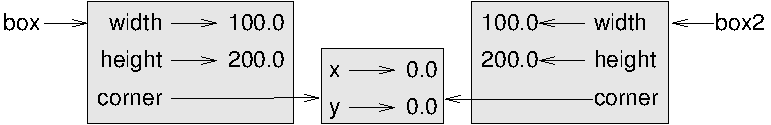
\includegraphics[scale = 0.8] {figs/rectangle2.pdf}}
\caption{diagrama de objeto.}
\label{} fig.rectangle2
\end{figure}

Figura ~ \ref {} fig.rectangle2 mostra o diagrama de objeto se parece.
\index{diagrama de estado}
\index{diagrama! Estado}
\index{diagrama objeto}
\index{diagrama! Objeto}
Esta operação é chamada de {cópia superficial \bf} porque ele copia os
objeto e todas as referências que ele contém, mas não os objetos incorporados.
\index{cópia superficial}
\index{cópia! Rasa}

Para a maioria das aplicações, não é isso que você quer. Neste exemplo,
invocando \verb "grow_rectangle" em um dos retângulos que não
afetar o outro, mas invocando \verb "move_rectangle" em ambos faria
afetar tanto! Este comportamento é confuso e propenso a erros.
\index{cópia profunda}
\index{cópia! Profundo}

Felizmente, a cópia {\tt} módulo contém um método chamado {\tt
deepcopy} que as cópias não apenas o objeto, mas também 
os objetos que ele se refere, e os objetos {\em que eles se referem a},
e assim por diante.
Você não vai se surpreender ao saber que esta operação é
chamado de {\bf cópia profunda}.
\index{function deepcopy}
\index{function! Deepcopy}

\begin{verbatim}
>>> Box3 = copy.deepcopy (box)
>>> Box3 caixa é
Falso
>>> Box3.corner é box.corner
Falso
\end{verbatim}
%
{\tt box3} e {caixa \tt} são objetos completamente separados.


\begin{} exercício

Escreva uma versão do \verb "move_rectangle" que cria e
retorna um novo retângulo em vez de modificar o antigo.

\end{} exercício


\section{} Depuração
\label{} hasattr
\index{depuração}

Quando você começar a trabalhar com objetos, você é provável encontrar
algumas novas exceções. Se você tentar acessar um atributo
que não existe, você recebe um {\tt AttributeError}:
\index{exceção! AttributeError}
\index{} AttributeError

\begin{verbatim}
>>> P = Ponto ()
>>> Print pz
AttributeError: instância Point tem nenhum atributo 'z'
\end{verbatim}
%
Se você não tiver certeza do tipo de um objeto é, você pode perguntar:
\index{type função}
\index{function! Tipo}

\begin{verbatim}
>>> Type (p)
<type'__main__.Point'>
\end{verbatim}
%
Se você não tem certeza se um objeto tem um atributo especial,
você pode usar a função built-in {\tt hasattr}:
\index{function hasattr}
\index{function! Hasattr}

\begin{verbatim}
>>> Hasattr (p, 'x')
Verdadeiro
>>> Hasattr (p, 'z')
Falso
\end{verbatim}
%
O primeiro argumento pode ser qualquer objeto, o segundo argumento é uma {\em
string} que contém o nome do atributo.


\section{} Glossário

\begin{description}

\item[classe]: Um tipo definido pelo usuário. A definição de classe cria um novo
classe de objeto.
\index{classe}

\[Objeto de classe:] Item Um objeto que contém informações sobre um
tipo definido pelo usuário. O objeto classe pode ser usada para criar instâncias
do tipo.
\index{classe de objeto}
\index{objeto! Classe}

\item[exemplo:] Um objeto que pertence a uma classe.
\index{instance}

\item[atributo:] Um dos valores nomeado associado a um objeto.
\index{atributo! Instance}
\index{atributo instance}

\item[incorporado (objeto):] Um objeto que é armazenado como um atributo
de outro objeto.
\index{objeto incorporado}
\index{objeto! Embutido}

\item[cópia superficial:] Para copiar o conteúdo de um objeto, incluindo
quaisquer referências a objetos embutidos;
implementado pelo {copy \tt} function no {copy \tt} módulo.
\index{cópia superficial}

\item[cópia profunda:] Para copiar o conteúdo de um objeto, bem como qualquer
objetos incorporados, e quaisquer objetos incorporados neles, e assim por diante;
implementado pelo {\tt deepcopy} function no {copy \tt} módulo.
\index{cópia profunda}

\[Diagrama de objetos:] item A diagrama que mostra objetos, sua
atributos, e os valores dos atributos.
\index{diagrama objeto}
\index{diagrama! Objeto}

\end{description}


\section{Exercícios}

\begin{} exercício
\label{tela}
\index{} Swampy
\index{módulo Mundo}
\index{módulo! Mundo}

Swampy (ver capítulo ~ \ref {turtlechap}) fornece um módulo chamado {\tt
  Mundo}, que define um tipo definido pelo usuário também chamado {\tt Mundo}.
Você pode importá-lo assim:

\begin{verbatim}
de swampy.World importação Mundo
\end{verbatim}

Ou, dependendo de como você instalou o Swampy, como este:

\begin{verbatim}
Mundial de importação Mundo
\end{verbatim}

O código a seguir cria um objeto Mundial e chamadas
o {\tt mainloop} método, que
espera para o usuário.

\begin{verbatim}
mundo = Mundo ()
world.mainloop ()
\end{verbatim}

Uma janela deve aparecer com uma barra de título e um quadrado vazio.
Vamos usar essa janela para desenhar pontos,
Retângulos e outras formas.  
Adicione as seguintes linhas antes de chamar
\Verb "mainloop" e execute o programa novamente.
\index{objeto Canvas}
\index{objeto! Canvas}

\begin{verbatim}
tela = world.ca (width = 500, height = 500, fundo = 'branco')
bbox = [[-150, -100], [150, 100]]
canvas.rectangle (bbox, esboço = 'black', width = 2, preencher = 'Green4')
\end{verbatim}

Você deverá ver um retângulo verde com um contorno preto.
A primeira linha cria uma tela, que aparece na janela
como um quadrado branco. O objeto Canvas fornece métodos como
{\tt retângulo} para desenhar várias formas.
\index{caixa delimitadora}

{\tt bbox} é uma lista de listas que representa o `` caixa delimitadora''
do retângulo. O primeiro par de coordenadas é o inferior esquerdo
canto do retângulo, o segundo par é o canto superior direito.

Você pode desenhar um círculo assim:

\begin{verbatim}
canvas.circle ([-25,0], 70, contorno = None, preencher = 'red')
\end{verbatim}

O primeiro parâmetro é o par de coordenadas para o centro do
círculo, o segundo parâmetro é o raio.

Se você adicionar essa linha para o programa, 
o resultado deve se parecer com a bandeira nacional de Bangladesh
(Ver \url{http://en.wikipedia.org/wiki/Gallery_of_sovereign-state_flags}).
\index{Bangladesh, bandeira nacional}

\begin{enumerate}

\item Escreva uma função chamada \verb "draw_rectangle" que leva um
  Lona e um retângulo como argumentos e desenha um
  representação do retângulo no Canvas.

\item Adicionar um atributo chamado {color \tt} para seus objetos de retângulo e
  modificar \verb "draw_rectangle" para que ele usa o atributo cor
  a cor de preenchimento.

\item Escreva uma função chamada \verb "draw_point" que leva um
  Lona e um Point como argumentos e desenha um
  representação do ponto na tela.

\item Definir uma nova classe chamada Círculo com atributos apropriados e
  instanciar alguns objetos círculo. Escreva uma função chamada
  \Verb "draw_circle" que desenha círculos na tela.
\index{República Checa, a bandeira nacional}

\item Escreva um programa que desenha a bandeira nacional da República Checa.
Dica: você pode desenhar um polígono assim:

\begin{verbatim}
pontos = [[-150, -100], [150, 100], [150, -100]]
canvas.polygon (pontos, preencher = 'blue')
\end{verbatim}

\end{enumerate}
\index{lista de cores}
\index{cores disponíveis}

Eu escrevi um pequeno programa que lista as cores disponíveis;
Você pode baixá-lo a partir de \url{http://thinkpython.com/code/color_list.py}.

\end{} exercício


\chapter{Classes e funções}
\label{tempo}

Os exemplos de código deste capítulo estão disponíveis a partir
\url{http://thinkpython.com/code/Time1.py}.

\section{hora}
\label{} time.object

Como outro exemplo de um tipo definido pelo usuário, vamos definir uma classe chamada
{\tt Tempo} que registra a hora do dia. A aparência de definição de classe
como esta:
\index{tipo definido pelo usuário}
\index{type! Definido pelo usuário}
\index{classe Time}
\{Tempo classe!} Índice

\begin{verbatim}
classe Time (object):
    "" "Representa o tempo de dia.
       
    atributos: hora, minuto, segundo
    "" "
\end{verbatim}
%
Podemos criar um novo {\tt Tempo} objeto e atribuir
atributos para horas, minutos e segundos:

\begin{verbatim}
tempo = Time ()
time.hour = 11
time.minute = 59
time.second = 30
\end{verbatim}
%
O diagrama de estado para o {\tt Tempo} objeto parece com a Figura ~ \ref {} fig.time.
\index{diagrama de estado}
\index{diagrama! Estado}
\index{diagrama objeto}
\index{diagrama! Objeto}

\begin{} exercício
\label{} ex.printtime

Escreva uma função chamada \verb "print_time" que leva um 
Objeto Tempo e imprime na forma {\tt hora: minuto: segundo}.
Dica: a seqüência de formato \verb "'.2 d'" imprime um inteiro usando
pelo menos dois dígitos, incluindo um zero à esquerda, se necessário.

\end{} exercício

\begin{} exercício
\label{} IsAfter
\index{função booleana}

Escreva uma função booleana chamada \verb "is_after" que
toma dois objetos de Tempo, {\tt t1} e {\tt t2}, e
retornos {\tt true} se {\tt t1} segue {\tt t2} em ordem cronológica e
{\tt false} contrário. Desafio: não use uma {\tt if}.
\end{} exercício

\begin{figure}
\centerline
{\includegraphics[scale = 0.8] {figos / time.pdf}}
\caption{diagrama de objeto.}
\label{} fig.time
\end{figure}


\section{funções Pure}
\index{protótipo e remendo}
\index{plano de desenvolvimento! Protótipo e remendo}

Nas próximas seções, vamos escrever duas funções que agregam tempo
valores. Eles demonstram dois tipos de funções: funções puras e
modificadores. Eles também demonstram um plano de desenvolvimento que eu vou chamar {\bf
  protótipo e remendo}, que é uma forma de combater um problema complexo
começando com um protótipo simples e incrementalmente lidar com o
complicações.

Aqui é um simples protótipo de \verb "add_time":

\begin{verbatim}
add_time def (T1, T2):
    sum = Time ()
    sum.hour = t1.hour + t2.hour
    sum.minute = t1.minute + t2.minute
    sum.second = t1.second + t2.second
    voltar soma
\end{verbatim}
%
A função cria um novo {\tt Tempo} objeto, inicializa sua
atributos e retorna uma referência para o novo objeto. Isto é chamado
uma {\bf pura função} porque não modificar qualquer um dos objetos
passado para ele como argumentos e não tem nenhum efeito,
como imprimir um valor ou pegar entrada do usuário, 
que não retornar um valor.
\index{pura função}
\index{type função! Puro}

Para testar essa função, eu vou criar dois objetos Time: {\tt início}
contém a hora de início de um filme, como {\em Monty Python eo
Santo Graal} e {duração \tt} contém o tempo de execução do filme,
que é uma hora 35 minutos.
\index{Monty Python eo Santo Graal}

\Verb "add_time" descobre quando o filme será feito.

\begin{verbatim}
>>> Start = Time ()
>>> Start.hour = 9
>>> Start.minute = 45
>>> Start.second = 0

>>> Duração = Time ()
>>> Duration.hour = 1
>>> Duration.minute = 35
>>> Duration.second = 0

>>> Feito = add_time (início, duração)
>>> Print_time (feito)
10:80:00
\end{verbatim}
%
O resultado, {\tt 10:80:00} pode não ser o que você estava esperando
para. O problema é que esta função não lida com casos em que o
número de segundos ou minutos, acrescenta-se a mais de sessenta anos. Quando isso
acontece, temos que levar ``'' os segundos extras para a coluna minuto
ou os minutos extras para a coluna hora.
\index{transporte, além de}

Aqui está uma versão melhorada:

\begin{verbatim}
add_time def (T1, T2):
    sum = Time ()
    sum.hour = t1.hour + t2.hour
    sum.minute = t1.minute + t2.minute
    sum.second = t1.second + t2.second

    se sum.second> = 60:
        sum.second - = 60
        sum.minute + = 1

    se sum.minute> = 60:
        sum.minute - = 60
        sum.hour + = 1

    voltar soma
\end{verbatim}
%
Embora esta função estiver correta, ela está começando a ficar grande.
Veremos uma alternativa mais curta depois.


\section{} Modificadores
\label{incremento}
\index{} modificador
\index{type função! Modificador}

Às vezes é útil para uma função para modificar os objetos que ela recebe como
parâmetros. Neste caso, as alterações são visíveis para o chamador.
Funções que trabalham desta forma são chamados de modificadores {\bf}.
\index{incremento}

{Tt incremento \}, o que acrescenta um determinado número de segundos para um {\tt Tempo}
objeto, pode ser escrito naturalmente como um
modificador. Aqui está um esboço:

\begin{verbatim}
incremento def (tempo, segundos):
    time.second + = segundos

    se time.second> = 60:
        time.second - = 60
        time.minute + = 1

    se time.minute> = 60:
        time.minute - = 60
        time.hour + = 1
\end{verbatim}
%
A primeira linha executa a operação básica; os negócios restantes
com os casos especiais que vimos antes.
\index{case especial}

É este o funcionamento correto? O que acontece se o parâmetro {\tt segundos}
é muito maior do que sessenta?  

Nesse caso, não é suficiente para levar
uma vez, temos que continuar fazendo isso até que {\tt time.second} é inferior a sessenta anos.
Uma solução é substituir o {\tt if} declarações com {\tt enquanto}
declarações. Isso faria com que a função correta, mas não
muito eficiente.

\begin{} exercício

Escreva uma versão correta do incremento {\tt} que
não contém quaisquer loops.

\end{} exercício

Tudo o que pode ser feito com modificadores pode também ser feito com puro
funções. De fato, algumas linguagens de programação permitem apenas puro
funções. Há algumas evidências de que os programas que usam puro
funções são mais rápidos para desenvolver e menos de programas propenso a erros
que os modificadores de uso. Mas modificadores são convenientes, às vezes,
e programas funcionais tendem a ser menos eficientes.

Em geral, eu recomendo que você escreva funções puras sempre que for
razoável e resort para modificadores somente se houver uma convincente
vantagem. Esta abordagem pode ser chamado de {\bf funcional
estilo de programação}.
\index{estilo de programação funcional}


\begin{} exercício

Escreva uma versão `` puro'' de {incremento \tt} que cria e retorna
um novo objeto de tempo em vez de modificar o parâmetro.

\end{} exercício


\section{Prototipagem contra planejamento}
\label{protótipo}
\index{protótipo e remendo}
\index{plano de desenvolvimento! Protótipo e remendo}
\index{desenvolvimento planejado}
\index{plano de desenvolvimento! Planejado}

O plano de desenvolvimento que estou demonstrando é chamado `` protótipo e
corrigir.'' Para cada função, escrevi um protótipo que realizou a
cálculo básico e, em seguida, testou-o, remendando os erros ao longo do
caminho.

Esta abordagem pode ser eficaz, especialmente se você ainda não tem um
profunda compreensão do problema. Mas correções incrementais podem
gerar o código que é desnecessariamente complicado --- uma vez que lida com
muitos casos especiais --- e --- não confiável, uma vez que é difícil saber se você
ter encontrado todos os erros.

Uma alternativa é {\bf desenvolvimento planejado}, em que de alto nível
visão sobre o problema pode tornar a programação mais fácil. Em
Neste caso, a percepção é que um objecto de tempo é realmente um número de três dígitos
número em base 60 (ver \url{http://en.wikipedia.org/wiki/Sexagesimal}.)! O
{\tt} segundo atributo é o `` coluna queridos,'' o {\tt minuto}
atributo é o `` coluna anos sessenta,'' eo {\tt hora} atributo é
o `` coluna trinta e seis centenas.''
\index{sexagesimal}

Quando escrevemos \verb "add_time" e {\tt incremento}, estávamos efetivamente
fazendo disso na base 60, que é por isso que tivemos de transportar de um
coluna para a próxima.
\index{transporte, além de}

Esta observação sugere uma outra abordagem para o problema todo --- nós
pode converter objetos Tempo para inteiros e tirar proveito do fato de
que o computador sabe como fazer aritmética inteira.  

Aqui está uma função que converte Times inteiros:

\begin{verbatim}
time_to_int def (tempo):
    minutos = time.hour * 60 + time.minute
    segundos = minutos * 60 + time.second
    retornar segundos
\end{verbatim}
%
E aqui é a função que converte inteiros para a Times
(Lembre-se que {divmod \tt} divide o primeiro argumento pelo segundo
e retorna o quociente eo resto como uma tupla).
\index{} divmod

\begin{verbatim}
int_to_time def (segundos):
    tempo = Time ()
    minutos, time.second = divmod (segundos, 60)
    time.hour, time.minute = divmod (minutos, 60)
    tempo de retorno
\end{verbatim}
%
Você pode ter que pensar um pouco, e fazer alguns testes, para convencer
mesmo que estas funções estão corretas. Uma maneira de testá-los é
verificar se \verb "time_to_int (int_to_time (x)) == x" para muitos valores de
{\tt x}. Este é um exemplo de uma verificação de consistência.
\index{verificação de consistência}

Uma vez que você está convencido de que eles estão corretos, você pode usá-los para 
reescrever \verb "add_time":

\begin{verbatim}
add_time def (T1, T2):
    = segundos time_to_int (t1) + time_to_int (t2)
    voltar int_to_time (segundos)
\end{verbatim}
%
Esta versão é mais curto do que o original, e mais fácil de verificar.

\begin{} exercício

Reescreva {incremento \tt} usando \verb "time_to_int" e \verb "int_to_time".

\end{} exercício

De certa forma, a conversão de base 60 para base 10 e voltar é mais difícil
do que simplesmente lidar com horários. Conversão de base é mais abstrata, a nossa
intuição para lidar com valores de tempo é melhor.

Mas se tivermos o discernimento para tratar vezes como base de 60 números e fazer
o investimento de escrever as funções de conversão (\verb "time_to_int"
e \verb "int_to_time"), temos um programa que é menor, mais fácil de
ler e depurar, e mais confiável.

É também mais fácil para adicionar funcionalidades depois. Por exemplo, imagine
subtraindo duas vezes para encontrar a duração entre elas. O
abordagem ingênua seria implementar subtração com empréstimo.
Usando as funções de conversão seria mais fácil e mais provável de ser
correta.
\index{subtração com empréstimo}
\index{empréstimo, subtração com}
\index{generalização}

Ironicamente, algumas vezes fazer um problema mais difícil (ou mais geral) torna
mais fácil (porque há menos casos especiais e menos oportunidades
de erro).


\section{} Depuração
\index{depuração}

Um objeto O tempo está bem formado se os valores de {\tt minutos} e {\tt
segundo} estão entre 0 e 60 (incluindo 0, mas não 60) e se 
{\tt hora} é positivo. {\tt hora} e {\tt minuto} deve ser
valores integrais, mas pode permitir que {\tt segundo} ter um
frações.
\index{} invariante

Requisitos como estes são chamados de invariantes {\bf} porque
eles devem sempre ser verdade. Para colocá-lo de forma diferente, se eles
não são verdadeiras, então algo está errado.

Escrever código para verificar os seus invariantes pode ajudá-lo a detectar erros
e encontrar suas causas. Por exemplo, você pode ter uma função
como \verb "valid_time" que leva um objeto Tempo e retorna
{\tt false} se violar um invariante:

\begin{verbatim}
valid_time def (tempo):
    se time.hour <0 ou time.minute <0 ou time.second <0:
        retornará False
    se time.minute> = 60 ou time.second> = 60:
        retornará False
    retornar True
\end{verbatim}
%
Então, no início de cada função você pode verificar o
argumentos para se certificar de que eles são válidos:
\index{elevar declaração}
\index{declaração! Raise}

\begin{verbatim}
add_time def (T1, T2):
    se não valid_time (t1) ou não valid_time (t2):
        levantar ValueError, 'inválido objeto Tempo em add_time'
    = segundos time_to_int (t1) + time_to_int (t2)
    voltar int_to_time (segundos)
\end{verbatim}
%
Ou você pode usar um {\tt assert} declaração, que verifica um dado invariante
e gera uma exceção se ele falhar:
\index{afirmar declaração}
\index{declaração! Assert}

\begin{verbatim}
add_time def (T1, T2):
    afirmam valid_time (t1) e valid_time (t2)
    = segundos time_to_int (t1) + time_to_int (t2)
    voltar int_to_time (segundos)
\end{verbatim}
%
{\tt assert} declarações são úteis porque distinguir
código que lida com condições normais de código
que verifica se há erros.


\section{} Glossário

\begin{description}

\item[protótipo e patch:] Um plano de desenvolvimento que envolve
escrever um rascunho de um programa, testando e corrigindo erros como
eles são encontrados.
\index{protótipo e remendo}

\item[desenvolvimento planejado:] Um plano de desenvolvimento que envolve
de alto nível, uma visão sobre o problema e mais planejamento do que incrementais
desenvolvimento ou o desenvolvimento do protótipo.
\index{desenvolvimento planejado}

\item[função pura:] Uma função que não modifica nenhum dos objetos que ela
recebe como argumentos. A maioria das funções puras é frutífera.
\index{pura função}

\item[modificador]: Uma função que muda um ou mais dos objetos que ela
recebe como argumentos. A maioria dos modificadores são infrutíferas.
\index{} modificador

\item[estilo de programação funcional:] Um estilo de programa em que o
maioria das funções são puras.
\index{estilo de programação funcional}

\item[invariante:] Uma condição que deve sempre ser verdade durante o
execução de um programa.
\index{} invariante

\end{description}


\section{Exercícios}

Os exemplos de código deste capítulo estão disponíveis a partir
\url{http://thinkpython.com/code/Time1.py}; soluções para estes
exercícios estão disponíveis em \url{http://thinkpython.com/code/Time1_soln.py}.

\begin{} exercício

Escreva uma função chamada \verb "mul_time" que leva um objeto Tempo
e um número e retorna um novo objeto que contém Tempo
o produto da Hora original eo número.

Em seguida, use \verb "mul_time" para escrever uma função que leva um tempo
objeto que representa o tempo de chegada de uma corrida, e um número
que representa a distância, e retorna um objeto que representa Tempo
o ritmo médio (tempo por quilômetro).
\index{ritmo execução}

\end{} exercício

\begin{} exercício
\index{Data classe}
\index{classe! Date}

Escrever uma definição de classe para um objeto Date que tem atributos {\tt
Dia}, {mês \tt} e {ano \tt}. Escreva uma função chamada
\Verb "increment_date" que leva um objeto de data, {data \tt} e um
Inteiro, {\tt n}, e retorna um novo objeto Date que
Representa o dia {\tt n} dias após {data \tt}. Dica:
`` Trinta dias tem setembro ...'' Desafio: faz a sua função
Lidar com os anos bissextos corretamente? Veja \url{http://en.wikipedia.org/wiki/Leap_year}.

\end{} exercício


\begin{} exercício
\index{módulo datetime}
\index{módulo! Datetime}

O {\tt datetime} módulo fornece {data \tt} e {TIME \tt} objetos
que são semelhantes aos objetos de data e hora neste capítulo, mas
eles fornecem um rico conjunto de métodos e operadores. Leia o
documentação em \url{http://docs.python.org/2/library/datetime.html}.

\begin{enumerate}

\item Use o {\tt datetime} módulo para escrever um programa que recebe o
  data e imprime o dia da semana atual.
\index{aniversário}

\item Escreva um programa que tem um aniversário como entrada e imprime o
  idade do usuário eo número de dias, horas, minutos e segundos até
  seu próximo aniversário.

\item Para duas pessoas que nasceram em dias diferentes, há um dia em que um
  é duas vezes mais velho que o outro. Essa é a sua Day duplo. Escreva uma
  programa que leva dois aniversários e calcula seu dia dobro.

\item Para um pouco mais desafio, escrever a versão mais geral que
  calcula o dia em que uma pessoa é de R $ n $ vezes mais velho que o outro.
\index{dia dobro}

\end{enumerate}

\end{} exercício


\chapter{Classes e métodos}

Os exemplos de código deste capítulo estão disponíveis a partir
\url{http://thinkpython.com/code/Time2.py}.

\section{recursos orientados a objetos}
\index{programação orientada a objeto}

Python é uma {\bf linguagem de programação orientada a objeto}, o que significa
que ele oferece recursos que suportam orientado a objeto
programação.

Não é fácil definir a programação orientada a objeto, mas temos
já vi algumas de suas características:

\begin{itemize}

\Programs itens são feitos de definições e função de objeto
definições, e a maior parte do cálculo é expresso em termos
de operações sobre objetos.

\item Cada definição de objeto corresponde a algum objeto ou conceito
no mundo real, e as funções que operam sobre o objeto
correspondem às formas de objetos do mundo real interagem.

\end{itemize}

Por exemplo, o {\tt Tempo} classe definida no capítulo ~ \ref {tempo}
corresponde ao modo como as pessoas gravar a hora do dia, e o
funções que definimos correspondem aos tipos de coisas que as pessoas fazem com
vezes. Da mesma forma, o {\tt Ponto} e {\tt Retângulo} aulas
correspondem aos conceitos matemáticos de um ponto e um retângulo.

Até agora, não temos aproveitado as características Python fornece a
suportar a programação orientada a objeto. Estes
recursos não são estritamente necessários, a maioria deles fornecer
sintaxe alternativa para as coisas que já fizemos. Mas, em muitos casos,
a alternativa é mais conciso e com mais precisão transmite a
estrutura do programa.

Por exemplo, na {\Tempo tt} programa, não há nenhuma óbvia
conexão entre a definição de classe e as definições de função
que se seguem. Com algum exame, é evidente que todas as funções
leva pelo menos um {\tt Tempo} objeto como um argumento.
\index{método}
\index{função}

Esta observação é a motivação para {métodos \bf}; um método é
uma função que está associada a uma determinada classe.
Vimos métodos para strings, listas, dicionários e tuplas.
Neste capítulo, vamos definir métodos para tipos definidos pelo usuário.
\index{} sintaxe
\index{} semântica

Os métodos são os mesmos que semanticamente funções, mas existem
duas diferenças sintáticas:

\begin{itemize}

\item Métodos são definidos dentro de uma definição de classe, a fim
para tornar a relação entre a classe e o método explícito.

\item A sintaxe para invocar um método é diferente do
sintaxe para chamar uma função.

\end{itemize}

Nas próximas seções, vamos dar as funções do anterior
dois capítulos e transformá-los em métodos. Esta transformação é
puramente mecânico, você pode fazê-lo simplesmente seguindo uma seqüência de
passos. Se você estiver confortável conversão de uma forma para outra,
você será capaz de escolher a melhor forma para o que você está fazendo.


\section{} objetos de impressão
\index{objeto! Impressão}

No capítulo ~ \ref {tempo}, definimos uma classe chamada
{\tt} Tempo e no Exercício ~ \ref {} ex.printtime, você 
escreveu uma função chamada \verb "print_time":

\begin{verbatim}
classe Time (object):
    "" "Representa o tempo de dia." ""

print_time def (tempo):
    print '.2 d:.2 d:.2 d'(time.hour, time.minute, time.second)
\end{verbatim}
%
Para chamar esta função, você tem que passar por um {\tt Tempo} objeto como um
argumento:

\begin{verbatim}
>>> Start = Time ()
>>> Start.hour = 9
>>> Start.minute = 45
>>> Start.second = 00
>>> Print_time (início)
09:45:00
\end{verbatim}
%
Para fazer \verb "print_time" um método, tudo o que temos a fazer é
mover a definição de função dentro da definição da classe. Aviso
a mudança de recuo.
\index{recuo}

\begin{verbatim}
classe Time (object):
    print_time def (tempo):
        print '.2 d:.2 d:.2 d'(time.hour, time.minute, time.second)
\end{verbatim}
%
Agora, há duas maneiras de chamar \verb "print_time". O primeiro
(E menos comum) maneira é usar sintaxe da função:
\index{f unção sintaxe}
\index{} a notação de ponto


\begin{verbatim}
>>> Time.print_time (início)
09:45:00
\end{verbatim}
%
Neste uso de notação de ponto, {\tt Tempo} é o nome da classe,
e \verbo "print_time" é o nome do método. {Start \tt} é
passado como um parâmetro.

A segunda (e mais conciso) maneira é usar a sintaxe do método:
\index{sintaxe do método}

\begin{verbatim}
>>> Start.print_time ()
09:45:00
\end{verbatim}
%
Nesta utilização de notação de ponto, \verbo "print_time" é o nome do
método (de novo), e {\tt início} é o objeto que o método é
invocada, que é chamado o assunto {\bf}. Assim como o
sujeito de uma frase é o que a frase é sobre, o assunto
de uma invocação de método é o que o método está em causa.
\index{assunto}

Dentro do método, o sujeito é atribuído ao primeiro
parâmetro, portanto, neste caso {\tt começar} é atribuído
para {tempo \tt}.
\index{self (nome do parâmetro)}
\index{parâmetro! Self}

Por convenção, o primeiro parâmetro de um método é
chamado {\tt self}, de modo que seria mais comum para escrever
\Verb "print_time" assim:

\begin{verbatim}
classe Time (object):
    print_time def (self):
        print '.2 d:.2 d:.2 d'(self.hour, self.minute, self.second)
\end{verbatim}
%
A razão para essa convenção é uma metáfora implícita:
\index{metáfora, invocação de método}

\begin{itemize}

\item A sintaxe para uma chamada de função, \verb "print_time (início)",
  sugere que a função é o agente ativo. Ele diz algo
  como, `` Ei \verb "print_time"! Aqui está um objeto para você imprimir.''

\item Na programação orientada a objetos, os objetos são o ativo
  agentes. A invocação de método como \verb "start.print_time ()", diz
  `` Ei {\tt começar}! Por favor, imprima-se.''

\end{itemize}

Essa mudança de perspectiva pode ser mais educado, mas não é óbvio
que é útil. Nos exemplos que vimos até agora, não pode
ser. Mas, por vezes, transferindo a responsabilidade das funções para o
objectos torna possível gravar funções mais versáteis, e faz
mais fácil de manter e reutilização de código.

\begin{} exercício
\label{convert}

Reescreva \verb "time_to_int" (da Seção ~ \ref {} protótipo) como um método.
Provavelmente não é apropriado para reescrever \verb "int_to_time" como um
método, o que objeto você invocá-lo em?

\end{} exercício


\section{Outro exemplo}
\index{incremento}

Aqui está uma versão de incremento {\tt} (da Seção ~ \ref {incremento})
reescrito como um método:

\begin{verbatim}
# Dentro Tempo de classe:

    incremento def (self, segundos):
        segundos + = self.time_to_int ()
        voltar int_to_time (segundos)
\end{verbatim}
%
Esta versão assume que \verb "time_to_int" é escrito
como um método, como no Exercício ~ \ref {} converter. Além disso, observe que
é uma função pura, e não um modificador.

Veja como você iria invocar {incremento \tt}:

\begin{verbatim}
>>> Start.print_time ()
09:45:00
>>> Finais = start.increment (1337)
>>> End.print_time ()
10:07:17
\end{verbatim}
%
O assunto, {\tt início}, é atribuído ao primeiro parâmetro,
{\tt self}. O argumento, {\tt 1337}, é atribuído ao
segundo parâmetro, segundo {\tt}.

Este mecanismo pode ser confuso, especialmente se você fizer um erro.
Por exemplo, se você invocar {incremento \tt} com dois argumentos, você
obter:
\index{exceção! TypeError}
\index{} TypeError

\begin{verbatim}
>>> Finais = start.increment (1337, 460)
TypeError: incremento () pega exatamente 2 argumentos (3 dado)
\end{verbatim}
%
A mensagem de erro é inicialmente confuso, porque há
apenas dois argumentos entre parênteses. Mas o assunto também é
considerado um argumento, para que todos juntos, que são três.


\section{Um exemplo mais complicado}

\Verb "is_after" (do Exercício ~ \ref {IsAfter}) é um pouco mais complicado
porque leva dois objetos Tempo como parâmetros. Neste caso, é
convencional para nomear o primeiro parâmetro {\tt self} ea segunda
parâmetro {\tt outro}:
\index{outro (nome do parâmetro)}
\index{parâmetro! Outros}

\begin{verbatim}
# Dentro Tempo de classe:

    def is_after (self, outro):
        retornar self.time_to_int ()> other.time_to_int ()
\end{verbatim}
%
Para usar esse método, você tem que chamá-lo em um objeto e passar
o outro como um argumento:

\begin{verbatim}
>>> End.is_after (início)
Verdadeiro
\end{verbatim}
%
Uma coisa legal sobre essa sintaxe é que quase lê
como o Inglês: `` final é depois começar''?


\section{O método init}
\index{método init}
\index{método! Inicialização}

O método init (abreviação de `` inicialização'') é
um método especial que é invocado quando um objeto é instanciado.  
Seu nome completo é \verbo "__init__" (dois caracteres de sublinhado,
seguido por {\tt inicialização}, e em seguida, mais dois sublinhados). Uma
método init para o {\tt} Tempo classe pode ter esta aparência:

\begin{verbatim}
# Dentro Tempo de classe:

    def __ init__ (self, horas = 0, minutos = 0, segundo = 0):
        self.hour = hora
        self.minute = minuto
        self.second = segundo
\end{verbatim}
%
É comum que os parâmetros de \verb "__init__"
ter os mesmos nomes dos atributos. A declaração

\begin{verbatim}
        self.hour = hora
\end{verbatim}
%
armazena o valor do parâmetro {\tt hora} como um atributo
de {\tt self}.
\index{parâmetro opcional}
\index{parâmetro! Opcional}
\index{value default}
\index{override}

Os parâmetros são opcionais, então se você chamar {\tt Tempo} com
sem argumentos, você obtém os valores padrão.

\begin{verbatim}
>>> Tempo = Time ()
>>> Time.print_time ()
00:00:00
\end{verbatim}
%
Se você fornecer um argumento, ele substitui {\tt hora}:

\begin{verbatim}
>>> Time = Tempo (9)
>>> Time.print_time ()
09:00:00
\end{verbatim}
%
Se você fornecer dois argumentos, eles substituem {\tt hora} e
{\tt minuto}.

\begin{verbatim}
>>> Time = Tempo (9, 45)
>>> Time.print_time ()
09:45:00
\end{verbatim}
%
E se você fornecer três argumentos, eles substituem os três
valores padrão.


\begin{} exercício
\{Classe Point} índice
\index{classe! Ponto}

Escrever um método init para o {\tt Ponto} classe que leva
{\tt x} e {\tt y} parâmetros como opcionais e cessionários
los para os atributos correspondentes.
\end{} exercício


\section{O método {\tt \_ \_str \_ \_}}
\index{método str @ \_ \_str \_ \_ método}
\index{método! \_ \_str \_ \_}

\Verb "__str__" é um método especial, como \verb "__init__",
que deve retornar uma representação de string de um objeto.
\{Representação string} índice

Por exemplo, aqui está uma {\tt str} método para objetos Time:

\begin{verbatim}
# Dentro Tempo de classe:

    def __ str__ (self):
        return '.2 d:.2 d:.2 d'(self.hour, self.minute, self.second)
\end{verbatim}
%
Quando você {\tt print} um objeto, Python invoca o {\tt str} método:
\index{declaração print}
\index{declaração! Print}

\begin{verbatim}
>>> Time = Tempo (9, 45)
>>> Tempo de impressão
09:45:00
\end{verbatim}
%
Quando eu escrevo uma nova classe, eu quase sempre começar por escrever 
\Verb "__init__", o que torna mais fácil para instanciar objetos, e 
\Verb "__str__", o que é útil para depuração.


\begin{} exercício

Escrever um {\tt str} método para o {\tt Ponto} class. Criar
um objeto Point e imprimi-lo.

\end{} exercício


\section{} Sobrecarga de operadores
\label{} operator.overloading

Ao definir outros métodos especiais, você pode especificar o comportamento
de operadores em tipos definidos pelo usuário. Por exemplo, se você definir
um método chamado \verb "__add__" para o {\tt Tempo} classe, você pode usar o
{\tt +} operador em objetos Tempo.

Aqui está o que a definição pode parecer:
\index{adicionar método}
\index{método! Add}

\begin{verbatim}
# Dentro Tempo de classe:

    def __ add__ (self, outro):
        segundos = self.time_to_int () + other.time_to_int ()
        voltar int_to_time (segundos)
\end{verbatim}
%
E aqui está como você pode usá-lo:

\begin{verbatim}
>>> Start = Time (9, 45)
>>> Duração = Time (1, 35)
>>> Duração inicial de impressão +
11:20:00
\end{verbatim}
%
Quando você aplica o {\tt +} operador objetos Time, invoca Python
\Verb "__add__". Quando você imprime o resultado, Python invoca
\Verb "__str__". Portanto, há muita coisa acontecendo nos bastidores!
\{} Sobrecarga de operador índice

Alterar o comportamento de um operador para que ele funcione com
tipos definidos pelo usuário é chamado de operador {\bf sobrecarga}. Para cada
operador em Python existe um método especial correspondente, como 
\Verb "__add__". Para mais detalhes, consulte
\url{http://docs.python.org/2/reference/datamodel.html # specialnames}.

\begin{} exercício

Escrever um {\tt add} método para a classe Point.  

\end{} exercício


\section{baseada Tipo expedição}

Na seção anterior, nós adicionamos dois objetos tempo, mas você
também pode querer adicionar um inteiro para um objeto Time. O
Segue-se uma versão do \verb "__add__"
que verifica o tipo de {\tt outro} e invoca ou
\Verb "add_time" ou {\tt incremento}:

\begin{verbatim}
# Dentro Tempo de classe:

    def __ add__ (self, outro):
        se isinstance (outro, Time):
            retorno self.add_time (outros)
        else:
            retorno self.increment (outros)

    def add_time (self, outro):
        segundos = self.time_to_int () + other.time_to_int ()
        voltar int_to_time (segundos)

    incremento def (self, segundos):
        segundos + = self.time_to_int ()
        voltar int_to_time (segundos)
\end{verbatim}
%
A função built-in {\tt isinstance} tem um valor e um
classe de objetos e retorna {\tt true} se o valor é uma instância
da classe.
\index{function isinstance}
\index{function! Isinstance}

Se {\tt outro} é um objeto Tempo, \verb "__add__" invoca
\Verb "add_time". Caso contrário, ele assume que o parâmetro
é um número e invoca {incremento \tt}. Esta operação é
chamado {expedição baseada tipo \bf} porque ele despacha o
computação de diferentes métodos de acordo com o tipo do
argumentos.
\index{expedição baseada tipo}
\{Baseada em tipo de expedição, índice}

Aqui estão alguns exemplos que usam o {\tt +} operador com diferentes
tipos:

\begin{verbatim}
>>> Start = Time (9, 45)
>>> Duração = Time (1, 35)
>>> Duração inicial de impressão +
11:20:00
>>> Print início + 1337
10:07:17
\end{verbatim}
%
Infelizmente, esta implementação de adição não é comutativa.
Se o número inteiro é o primeiro operando, você começa
\index{} comutatividade

\begin{verbatim}
>>> Print 1337 + início
TypeError: tipo operando sem suporte (s) para +: 'int' e 'exemplo'
\end{verbatim}
%
O problema é que, em vez de pedir o objeto Hora de adicionar um número inteiro,
Python está pedindo um inteiro para adicionar um objeto de tempo, e ele não sabe
como fazer isso. Mas há uma solução inteligente para este problema: a
especial método \verb "__radd__", que significa `` add do lado direito.''
Este método é chamado quando um objeto Tempo aparece no lado direito da
o {\tt +} operador. Aqui está a definição:
\index{método radd}
\index{método! Radd}

\begin{verbatim}
# Dentro Tempo de classe:

    def __ radd__ (self, outro):
        retorno self.__add__ (outros)
\end{verbatim}
%
E aqui está como ele é usado:

\begin{verbatim}
>>> Print 1337 + início
10:07:17
\end{verbatim}
%

\begin{} exercício

Escrever um {\tt add} método de Pontos que funciona com qualquer um
Objeto Point ou uma tupla:  

\begin{itemize}

\item Se o segundo operando é um ponto, o método deve retornar um novo
Ponto cujo $ $ x coordenada é a soma dos x $ $ coordenadas do
operandos, e da mesma forma para o $ $ y coordenadas.

\item Se o segundo operando é uma tupla, o método deve adicionar o
primeiro elemento do tuplo para o x $ $ coordenadas e a segunda
elemento para o $ $ y coordenar e retornar um novo ponto com o resultado. 

\end{itemize}

\end{} exercício

\section{} Polimorfismo

Envio à base de Tipo é útil quando é necessário, mas (felizmente)
nem sempre é necessário. Muitas vezes você pode evitá-lo por escrito funções
que funcionam corretamente para argumentos com tipos diferentes.
\index{expedição baseada tipo}
\{Baseada em tipo de envio!} Índice

Muitas das funções que nós escrevemos para cordas vai realmente
trabalhar para qualquer tipo de sequência.
Por exemplo, na secção ~ \ref {histograma}
utilizou-{\tt histograma} para contar o número de vezes que cada letra
aparece em uma palavra.

\begin{verbatim}
histograma (s) def:
    d = dict ()
    para c em s:
        se c não em d:
            d [c] = 1
        else:
            d [c] = d [c] +1
    voltar d
\end{verbatim}
%
Esta função também funciona para listas, tuplas, dicionários e até mesmo,
enquanto os elementos de {\tt s} são Hashable, para que eles possam ser usados
como chaves em {\tt d}.

\begin{verbatim}
>>> T = ['spam', "ovo", "spam", "spam", "bacon", "spam"]
>>> Histograma (t)
{'Toucinho': 1, 'ovo': 1, 'spam': 4}
\end{verbatim}
%
Funções que pode trabalhar com vários tipos são chamados de {\bf polimórfico}.
Polimorfismo pode facilitar a reutilização de código. Por exemplo, o built-in
função {\tt soma}, o que aumenta os elementos de uma seqüência, obras
enquanto os elementos de suporte a adição de sequência.
\index{polimorfismo}

Desde objetos Tempo fornecer uma {\tt add} método, eles trabalham
com {soma \tt}:

\begin{verbatim}
>>> T1 = Time (7, 43)
>>> T2 = Time (7, 41)
>>> T3 = Time (7, 37)
>>> Total = soma ([t1, t2, t3])
>>> Print total de
23:01:00
\end{verbatim}
%
Em geral, se todas as operações dentro de uma função 
trabalhar com um dado tipo, então a função funciona com esse tipo.

O melhor tipo de polimorfismo é o tipo intencional, onde
você descobre que uma função que você já escreveu pode ser
aplicado a um tipo que nunca planejado.


\section{} Depuração
\index{depuração}

É legal para adicionar atributos aos objetos em qualquer ponto na execução
de um programa, mas se você é um defensor da teoria dos tipos, é uma
prática duvidosa de ter objetos do mesmo tipo com diferentes
conjuntos de atributos. Geralmente é uma boa idéia
inicializar todos de uma objetos atributos no método init.
\index{método init}
\index{atributo! Inicializar}

Se você não tem certeza se um objeto tem um atributo específico, você
pode usar a função built-in {\tt hasattr} (ver Seção ~ \ref {hasattr}).
\index{function hasattr}
\index{function! Hasattr}
\index{atributo dict @ \_ \_dict \_ \_ atributo}
\index{atribuem! \_ \_dict \_ \_}

Outra forma de acessar os atributos de um objeto é através da
atributo especial \verb "__dict__", que é um dicionário que mapeia
atribuir nomes (como strings) e valores:

\begin{verbatim}
>>> P = Ponto (3, 4)
>>> Print p.__dict__
{'Y': 4, 'x': 3}
\end{verbatim}
%
Para fins de depuração, você pode achar que é útil para manter esta
função útil:

\begin{verbatim}
print_attributes DEF (obj):
    para attr em obj.__dict__:
        impressão attr, getattr (obj, attr)
\end{verbatim}
%
\verb "print_attributes" percorre os itens no dicionário do objeto
e impressões de cada nome de atributo e seu valor correspondente.
\index{travessia! Dicionário}
\index{dicionário! Travessia}

A função built-in {\tt getattr} leva um objeto e um atributo
Nome (como uma string) e retorna o valor do atributo.
\index{função getattr}
\index{function! Getattr}


\section{interface e implementação}

Um dos objetivos do projeto orientado a objetos é tornar o software mais
sustentável, o que significa que você pode manter o funcionamento do programa quando
outras partes da mudança de sistema, e modificar o programa para atender novo
requisitos.
\index{Interface}
\index{implementação}
\index{} sustentável
\index{projeto orientado a objetos}

Um princípio de design que ajuda a atingir esse objetivo é manter
interfaces de separar implementações. Para objetos, o que significa
que os métodos de uma classe fornece não deve depender de como o
atributos são representados.
\index{atributo}

Por exemplo, neste capítulo, desenvolvemos uma classe que representa
uma hora do dia. Métodos fornecidos por esta classe incluem
\Verb "time_to_int", \verb "is_after" e \verb "add_time".

Poderíamos implementar esses métodos de várias maneiras. Os detalhes do
implementação dependerá de como nós representamos tempo. Neste capítulo, o
atributos de um {\tt Tempo} objeto são {\tt hora}, {\tt minutos}, e
{\tt segundo}.

Como alternativa, poderíamos substituir esses atributos com
um único número inteiro que representa o número de segundos
desde a meia-noite. Esta implementação faria alguns métodos,
como \verb "is_after", mais fácil de escrever, mas faz alguns métodos
mais difícil.

Depois de implantar uma nova classe, você pode descobrir uma melhor
implementação. Se outras partes do programa estão a utilizar o seu
classe, que pode ser demorado e sujeito a erros para alterar o
interface.  

Mas, se você projetou a interface com cuidado, você pode
alterar a aplicação, sem alterar a interface, que
significa que as outras partes do programa não tem que mudar.

Mantendo a interface separada da aplicação significa que
você tem que esconder os atributos. Código de outras partes do programa
(Fora da definição de classe) deve usar métodos para ler
e modificar o estado do objecto. Eles não devem acessar o
atributos directamente. Este princípio é chamado {informação \bf escondendo};
ver \url{http://en.wikipedia.org/wiki/Information_hiding}.
\index{esconder informações}

\begin{} exercício

Faça o download do código deste capítulo
(\url{http://thinkpython.com/code/Time2.py}). Altere os atributos
de {\Tempo tt} para ser um único inteiro representando segundos desde
meia-noite. Em seguida, modificar os métodos (e da função
\Verb "int_to_time") para trabalhar com a nova implementação. Você deveria
não tem que modificar o código de teste no {\tt principal}. Quando estiver pronto,
a saída deveria ser o mesmo que antes. Solução:
\url{http://thinkpython.com/code/Time2_soln.py}

\end{} exercício


\section{} Glossário

\begin{description}

\item[linguagem orientada a objetos:] Uma linguagem que fornece recursos,
  como classes definidas pelo usuário e sintaxe do método, que facilitam
  programação orientada a objetos.
\index{linguagem orientada a objetos}

\item[programação orientada a objetos:] Um estilo de programação no qual
de dados e as operações que manipulam estão organizados em classes
e métodos.
\index{programação orientada a objeto}

\item[método:] Uma função que é definida dentro de uma definição de classe e
é chamado em instâncias dessa classe.
\index{método}

\item[subject:] O ​​objeto de um método é chamado em.
\index{assunto}

\[Sobrecarga de operadores:] item de Mudar o comportamento de um operador como
{\tt +} para que ele funciona com um tipo definido pelo usuário.
\index{sobrecarga}
\index{operador! Sobrecarga}

\item[baseada em tipo de expedição:] Um padrão de programação que verifica o tipo
de um operando e invoca funções diferentes para tipos diferentes.
\index{expedição baseada tipo}

\item[polimórfico:] Pertencente a uma função que pode trabalhar com mais
  de um tipo.  
\index{polimorfismo}

\[Esconder informações:] artigo O princípio de que a interface fornecida 
por um objeto não deve depender de sua execução, em especial
a representação de seus atributos.
\index{esconder informações}


\end{description}

\section{Exercícios}

\begin{} exercício
\index{valor padrão! Evitando mutável}
\index{objeto mutável, como valor default}
\index{pior erro}
\index{bug! Pior}
\index{classe Kangaroo}
\index{classe! Kangaroo}

Este exercício é um conto preventivo sobre um dos mais
comum e difícil de encontrar, erros no Python.
Escreva uma definição para uma classe chamada {\tt Kangaroo} com a seguinte
métodos:

\begin{enumerate}

Verbo método "__init__" \item Uma \que inicializa um atributo chamado 
\verb "pouch_contents" para uma lista vazia.

\item Um método chamado \verb "put_in_pouch" que leva um objeto
de qualquer tipo e adiciona-lo para \verb "pouch_contents".

\Verb método item A \"__str__" que retorna uma representação de cadeia
do objecto canguru e o conteúdo da bolsa.

\end{enumerate}
%
Teste seu código 
através da criação de duas {\tt Canguru} objetos, atribuindo-lhes a variáveis
chamado {\tt kanga} e {\tt roo} e, depois adicionando {\tt roo} para o
conteúdo do {\tt kanga} 's bolsa.

Download \url{http://thinkpython.com/code/BadKangaroo.py}. Contém
uma solução para o problema anterior com uma grande, erro desagradável.
Encontrar e corrigir o bug.

Se você ficar preso, você pode baixar
\url{http://thinkpython.com/code/GoodKangaroo.py}, o que explica a
problema e demonstra uma solução.
\index{aliasing}
\index{objeto incorporado}
\index{objeto! Embutido}

\end{} exercício




\begin{} exercício
\index{módulo Visual}
\index{módulo! Visual}
\index{módulo vpython}
\index{módulo! Vpython}

Visual é um módulo Python que fornece gráficos 3-D. É
nem sempre incluídos em uma instalação do Python, então você pode ter
para instalá-lo a partir de seu repositório de software ou, se ele não está lá,
de \url{vpython.org}.

O exemplo a seguir cria um espaço 3-D, que é de 256 unidades
de largura, comprimento e altura, e define o centro ``'' ser o
ponto $ (128128128) $. Em seguida, ele desenha uma esfera azul.

\begin{verbatim}
a partir do Visual import *

scene.range = (256, 256, 256)
scene.center = (128, 128, 128)

color = (0,1, 0,1, 0,9) # principalmente azul
esfera (pos = scene.center, raio = 128, color = cor)
\end{verbatim}

{\Color tt} é uma tupla RGB, ou seja, os elementos são Vermelho-Verde-Azul
níveis entre 0,0 e 1,0 (ver
\url{http://en.wikipedia.org/wiki/RGB_color_model}).

Se você executar este código, você deve ver uma janela com um preto
fundo e uma esfera azul. Se você arrastar o botão do meio
cima e para baixo, você pode zoom in e out. Você também pode girar
a cena, arrastando o botão direito, mas com apenas um
esfera do mundo, é difícil dizer a diferença.

O circuito a seguir cria um cubo de esferas:

\begin{verbatim}
t = intervalo (0, 256, 51)
para x em t:
    para y em t:
        para z em t:
            pos = x, y, z
            esfera (pos = pos, raio = 10, color = cor)
\end{verbatim}

\begin{enumerate}

\item Coloque esse código em um script e ter certeza que trabalha para
você.

\item Modifique o programa de modo que cada esfera no cubo
tem a cor que corresponde à sua posição no espaço RGB.
Note-se que as coordenadas estão dentro do intervalo de 0 - 255, mas
as tuplas RGB estão na faixa de 0.0 - 1.0.
\index{lista de cores}
\index{cores disponíveis}

\item Download \url{http://thinkpython.com/code/color_list.py}
e usar a função \verb "read_colors" para gerar uma lista
das cores disponíveis em seu sistema, os seus nomes e
Valores RGB. Para cada cor nomeada desenhar uma esfera na
posição que corresponde aos seus valores RGB.



\end{enumerate}

Você pode ver a minha solução em \url{http://thinkpython.com/code/color_space.py}.

\end{} exercício


\chapter{} Herança

Neste capítulo, apresento classes para representar cartas de baralho,
baralhos de cartas, e as mãos de poker. Se você não jogar poker, você pode
ler sobre ele em \url{http://en.wikipedia.org/wiki/Poker}, mas você não tem
a, eu vou dizer o que você precisa saber para os exercícios.
Os exemplos de código deste capítulo estão disponíveis a partir
\url{http://thinkpython.com/code/Card.py}.
\index{cartão de jogo, anglo-americano}
\index{cartão, jogo}
\index{} pôquer

Se você não estiver familiarizado com anglo-americanos cartas de baralho,
você pode ler sobre eles em \url{http://en.wikipedia.org/wiki/Playing_cards}.


\{} Objetos Cartão seção

Há cinquenta e duas cartas em um baralho, cada um deles pertence a uma das
quatro ternos e um dos treze fileiras. Os naipes são Espadas, Copas,
Diamantes e Clubes (em ordem decrescente em ponte). As fileiras são
Ás, 2, 3, 4, 5, 6, 7, 8, 9, 10, Valete, Rainha e Rei. Dependendo
o jogo que você está jogando, um Ás pode ser maior do que o rei
ou inferior a 2.
\index{} classificação
\index{terno}

Se quisermos definir um novo objeto para representar uma carta de baralho, é
óbvio que os atributos devem ser: {\tt classificação} e
{Tt terno \}. Não é tão óbvio que tipo os atributos
deve ser. Uma possibilidade é usar strings contendo palavras como
\Verb "" Spade "para ternos e \verb" 'Queen' "para fileiras. Um problema com
esta aplicação é que não seria fácil de cartões para comparar
ver que tinha um posto mais alto ou terno.
\index{} codificar
\index{} criptografar
\index{mapa para}
\index{representação}

Uma alternativa é usar inteiros para {\bf} codificar as fileiras e ternos.
Neste contexto, `` codificar'' significa que vamos definir um mapeamento
entre os números e fatos, ou entre números e fileiras. Este
tipo de codificação não se destina a ser um segredo (que
seria `` criptografia'').

\Newcommand {\mymapsto} {$ \mapsto $}

Por exemplo, esta tabela mostra os fatos e o número inteiro correspondente
códigos:

\begin{tabular} {lcl}
Spades & \mymapsto & 3 \\
Corações & \mymapsto & 2 \\
Diamonds & \mymapsto & 1 \\
Clubes e \mymapsto & 0
\end{tabular}

Este código faz com que seja fácil de comparar cartões, porque ternos maiores mapear para
números mais altos, podemos comparar fatos, comparando seus códigos.

O mapeamento por fileiras é bastante óbvio; cada uma das fileiras numéricos
mapas para o número inteiro correspondente e para cartões de face:

\begin{tabular} {lcl}
Jack & \mymapsto e 11 \\
Queen & \mymapsto & 12 \\
King & \mymapsto & 13 \\
\end{tabular}

Eu estou usando o \mymapsto ~ símbolo para deixar claro que esses mapeamentos
não fazem parte do programa Python. Eles fazem parte do programa
projetar, mas eles não aparecem explicitamente no código.
\{Classe} Cartão índice
\index{classe! Cartão}

A definição de classe para {\tt Cartão} parece com isso:

\begin{verbatim}
Cartão de classe (objeto):
    "" "Representa uma carta de baralho padrão." ""

    def __ init__ (self, terno = 0, rank = 2):
        self.naipe = terno
        self.posicao = posto
\end{verbatim}
%
Como de costume, o método init leva um opcional
parâmetro para cada atributo. O cartão padrão é
o 2 de Paus.
\index{método init}
\index{método! Inicialização}

Para criar um cartão, você chama {Card \tt} com a
terno e classificação do cartão que você deseja.

\begin{verbatim}
queen_of_diamonds = Card (1, 12)
\end{verbatim}
%


\{} Atributos de classe seção
\label{} class.attribute
\{Atributo da classe} índice
\index{atributo! Classe}

A fim de imprimir objetos Carta de uma forma que as pessoas podem facilmente
ler, precisamos de um mapeamento dos códigos inteiros para o correspondente
fileiras e ternos. Uma maneira natural de
fazer isso é com listas de strings. Nós atribuímos estas listas para {class \bf
atributos}:

\begin{verbatim}
# Cartão de classe dentro:

    suit_names = [, 'Diamonds' 'clubes', 'Corações', 'Spades']
    rank_names = [None, 'Ace', '2 ', '3', '4 ', '5', '6 ', '7', 
              '8 ', '9', '10 ',' Jack ',' Queen ',' King ']

    def __ str__ (self):
        return 's des'(Card.rank_names [self.posicao]
                             Card.suit_names [self.naipe])
\end{verbatim}
%
Variáveis ​​como \verb "suit_names" e \verb "rank_names", que são
definido dentro de uma classe, mas fora de qualquer método, são chamados
atributos de classe, porque eles estão associados ao objeto de classe 
{Tt Card \}.
\index{atributo instance}
\index{atributo! Instance}

Este termo distingue-os de variáveis ​​como {\tt terno} e {\tt
  Ranking}, que são chamados de {instance \bf atributos}, porque eles são
associado a uma instância particular.
\index{} a notação de ponto

Ambos os tipos de atributo são acessados ​​usando a notação de ponto. Para
exemplo, no \verb "__str__", {\tt self} é um objeto Card,
e {\tt self.posicao} é o seu rank. Do mesmo modo, {cartão \tt}
é um objeto de classe, e \verb "Card.rank_names" é um
lista de strings associados à classe.

Cada cartão tem seu próprio terno {\tt} e {\tt classificação}, mas não
é apenas uma cópia de \verb "suit_names" e \verb "rank_names".

Juntando tudo, a expressão
\verb "Card.rank_names [self.posicao]" significa `` usar o atributo {\tt classificação}
do objeto {\tt self} como um índice para a lista de \verb "rank_names"
do {Card \tt} classe e selecione o valor apropriado.''

O primeiro elemento da \verbo "rank_names" é {\tt Nenhum} porque não
nenhum cartão com grau zero. Ao incluir {\tt Nenhum} como um lugar-keeper,
temos um mapeamento com a propriedade agradável que o índice de dois mapas para o
corda \verb "'2 '", e assim por diante. Para evitar este tweak, poderíamos ter
utilizado um dicionário, em vez de uma lista.

Com os métodos que temos até agora, podemos criar e imprimir cartões:

\begin{verbatim}
>>> Card1 = Card (2, 11)
>>> Print card1
Jack of Hearts
\end{verbatim}

\begin{figure}
\centerline
{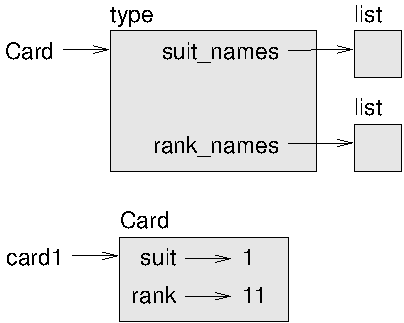
\includegraphics[scale = 0.8] {figs/card1.pdf}}
\caption{diagrama de objeto.}
\label{} fig.card1
\end{figure}

Figura ~ \ref {} fig.card1 é um diagrama da {Card \tt} objeto de classe
e um cartão de instância.
\index{diagrama de estado}
\index{diagrama! Estado}
\index{diagrama objeto}
\index{diagrama! Objeto}
{Card \tt} é um objeto de classe, por isso tem digitar {type \tt}. {\tt
card1} tem o tipo {Card \tt}. (Para economizar espaço, eu não chamar a
conteúdo de \verb "suit_names" e \verb "rank_names").


\section{Comparando cartões}
\label{} comparecard
\index{operador! Relacional}
\index{operador relacional}

Para os tipos de embutidos, há operadores relacionais
({\tt <}, {\tt>}, {\tt ==}, etc)
que compara
valores e determinar quando uma for maior do que, menos do que, ou igual a
outro. Para tipos definidos pelo usuário, que pode substituir o comportamento de
o built-in operadores, fornecendo um método chamado
\Verb "__cmp__".  

\Verb "__cmp__" tem dois parâmetros, {\tt auto} e {\tt outros},
e retorna um número positivo se o primeiro objeto for maior, um
número negativo se o segundo objeto é maior, e 0 se eles são
iguais uma à outra.
\index{override}
\{} Sobrecarga de operador índice

A ordem correta para os cartões não é óbvia.
Por exemplo, o qual
é melhor, o 3 de Paus ou o 2 de Ouros? Um deles tem um maior
classificar, mas o outro tem um naipe maior. A fim de comparar
cartões, você tem que decidir se posto ou terno é mais importante.

A resposta pode depender de qual jogo você está jogando, mas para manter
coisas simples, vamos fazer a escolha arbitrária que terno é mais
importante, por isso todos os Spades superará todos os diamantes,
e assim por diante.
\index{método cmp @ \_ \_cmp \_ \_ método}
\index{método! \_ \_cmp \_ \_}

Com essa decisão, podemos escrever \verb "__cmp__":

\begin{verbatim}
# Cartão de classe dentro:

    def __ cmp__ (self, outro):
        # Verificar os fatos
        se self.naipe> other.suit: retornar 1
        se self.naipe <other.suit: retornar -1

        # fatos são os mesmos ... verificar fileiras
        se self.posicao> other.posicao: retornar 1
        se self.posicao <other.posicao: retornar -1

        # fileiras são os mesmos ... é um empate
        retornar 0    
\end{verbatim}
%
Você pode escrever isso de forma mais concisa usando a comparação tupla:
\index{tupla Comparação}
\index{comparação! Tupla}

\begin{verbatim}
# Cartão de classe dentro:

    def __ cmp__ (self, outro):
        t1 = self.naipe, self.posicao
        t2 = other.suit, other.posicao
        retorno cmp (t1, t2)
\end{verbatim}
%
A função built-in {\tt cmp} tem a mesma interface
o método \verb "__cmp__": leva dois valores e retorna
um número positivo se a primeira for maior, um número negativo
se a segunda é maior, e 0, se eles forem iguais.
\index{function cmp}
\index{function! Cmp}

Em Python 3, {\tt cmp} não existe mais, eo \verb "__cmp__"
método não é suportado. Em vez disso, você deve fornecer \verb "__lt__",
que retorna {\tt true} se {\tt self} é menor que {\tt outro}.
Você pode implementar \verb "__lt__" usando tuplas e \verb "<"
operador.

\begin{} exercício

Escrever um verbo método "__cmp__" \Tempo para objetos. Dica: você
pode usar comparação tupla, mas você também pode considerar o uso
subtração inteiro.

Def __ cmp__ (self, outro):
Time_to_int retorno (self) - time_to_int (outros)

Se{\tt self} é mais tarde do que {\tt outro}, o resultado é
Um número positivo. Se {\tt outro} é mais tarde, o resultado
É negativo. E se {\tt self} e {\tt outro} são iguais
(Mas não necessariamente iguais)
O resultado é zero.

\end{} exercício


\section{} Decks
\index{list! Dos objetos}
\index{baralho, cartas de baralho}

Agora que temos cartões, o próximo passo é definir Decks. Uma vez que um
plataforma é composta de cartas, é natural que cada plataforma para conter um
lista de cartões como um atributo.
\index{método init}
\index{método! Inicialização}

O seguinte é uma definição de classe para {\tt plataforma}. O
método init cria o atributo {cartões \tt} e gera
o padrão estabelecido de cinquenta e duas cartas:
\index{composição}
\index{laço! Aninhada}
\index{classe Baralho}
\index{classe! Plataforma}

\begin{verbatim}
classe Deck (object):

    def __ init__ (self):
        self.cartas = []
        para atender na faixa (4):
            para classificação no intervalo (1, 14):
                cartão = Card (terno, classificação)
                self.cards.append (cartão)
\end{verbatim}
%
A maneira mais fácil para preencher o baralho é com um loop aninhado. O exterior
laço enumera os naipes de 0 a 3. O laço interno enumera o
classifica de 1 a 13. Cada iteração
cria um novo cartão com o terno e atual posição,
eo acrescenta a {\tt self.cartas}.
\index{método append}
\index{método! Append}


\section{Imprimindo o baralho}
\label{} imprimirBaralho
\index{método str @ \_ \_str \_ \_ método}
\index{método! \_ \_str \_ \_}

Aqui é um verbo método "__str__" \para {\tt plataforma}:

\begin{verbatim}
# Dentro classe Baralho:

    def __ str__ (self):
        res = []
        para cartão de self.cartas:
            res.append (str (cartão))
        retorno '\n'. join (res)
\end{verbatim}
%
Este método demonstra uma maneira eficiente para acumular uma grande
string: a construção de uma lista de strings e em seguida, usando {\tt juntar}.
A função built-in {\tt str} invoca o \verb "__str__"
método em cada cartão e retorna a representação de string.
\index{acumulador! String}
\index{string! Acumulador}
\index{método join}
\index{método! Juntar}
\index{newline}

Desde que invocar {\tt juntar} em um caractere de nova linha, as cartas
são separadas por novas linhas. Aqui está o que o resultado se parece com:

\begin{verbatim}
>>> Baralho = Deck ()
>>> Baralho impressão
Ás de Paus
2 de Paus
3 de Paus
...
10 de Espadas
Jack of Spades
Queen of Spades
Rei de Espadas
\end{verbatim}
%
Mesmo que o resultado aparece em 52 linhas, é
uma longa cadeia que contém novas linhas.


\section{Adicionar, remover shuffle e tipo}

Para lidar cartões, gostaríamos de um método que
retira uma carta do baralho e retorna.
O método lista {\tt pop} fornece uma maneira conveniente de fazer isso:
\{Método pop} índice
\index{método! Pop}

\begin{verbatim}
# Dentro classe Baralho:

    pop_card def (self):
        retornar self.cards.pop ()
\end{verbatim}
%
Desde {\tt pop} remove o {\em última} cartão na lista, estamos
tratar a partir da parte inferior do convés. Na vida real `` tráfico de fundo'' é
desaprovado,
mas, neste contexto, está ok.
\index{método append}
\index{método! Append}

Para adicionar um cartão, podemos usar o método de lista {\tt append}:

\begin{verbatim}
# Dentro classe Baralho:

    add_card def (self, cartão):
        self.cards.append (cartão)
\end{verbatim}
%
Um método como este que utiliza outra função sem fazer
muito trabalho real é às vezes chamado de verniz {\bf}. A metáfora
vem de madeira, onde é comum a cola uma fina
camada de madeira de boa qualidade da superfície de uma peça de barata
madeira.
\index{verniz}

Neste caso, estamos definindo um método `` fino'' que expressa
uma operação de lista em termos que são apropriados para decks.

Como outro exemplo, podemos escrever um método Baralho chamado {\tt Shuffle}
utilizando a função {\tt Shuffle} do {random \tt} módulo:
\index{módulo random}
\index{módulo! Random}
\index{função Shuffle}
\index{function! Shuffle}

\begin{verbatim}
# Dentro classe Baralho:
            
    def shuffle (self):
        random.shuffle (self.cartas)
\end{verbatim}
%
Não se esqueça de importar {\tt random}.

\begin{} exercício
\{} Método de classificação do índice
\index{método! Tipo}

Escreva um método Baralho chamado {\tt} tipo que usa o método de lista
{\tt tipo} para ordenar os cartões em uma {\tt plataforma}. {\tt Colecção} usos
o verbo método \"__cmp__" nós definido para determinar a ordem de classificação.
\end{} exercício



\section{} Herança
\index{herança}
\index{programação orientada a objeto}

O recurso de linguagem mais frequentemente associado com orientação a objetos
programação é {\bf herança}. Herança é a capacidade de
definir uma nova classe que é uma versão modificada de um existente
classe.
\index{classe pai}
\index{classe filha}
\index{classe! Criança}
\index{subclasse}
\index{superclasse}

Ele é chamado de `` herança'' porque a nova classe herda a
métodos da classe existente. Estendendo essa metáfora, o existente
classe é chamado o pai {\bf} ea nova classe é
chamou o filho {\bf}.

Como exemplo, vamos dizer que queremos uma classe para representar um `` lado,''
isto é, o conjunto de cartões realizada por um jogador. Uma mão é semelhante a um
convés: ambos são compostos de um conjunto de cartas e ambos requerem operações
como adição e remoção de cartões.

A mão também é diferente de um baralho, há operações que queremos para
mãos que não fazem sentido para uma plataforma. Por exemplo, em que o poker
pode comparar as duas mãos para ver qual deles ganha. Na ponte, poderíamos
computar uma pontuação para uma mão, a fim de fazer uma oferta.

Esta relação entre as classes --- semelhante, mas diferentes: --- empresta
se a herança.  

A definição de uma classe filha é como outras definições de classe,
mas o nome da classe pai aparece entre parênteses:
\index{parênteses! Classe pai em}
\index{classe pai}
\index{classe! Pai}
\index{classe Mão}
\index{classe! Mão}

\begin{verbatim}
classe Mao (Baralho):
    "" "Representa uma mão de cartas de jogar." ""
\end{verbatim}
%
Esta definição indica que {\tt Mão} herda {\tt plataforma};
isso significa que podemos usar métodos como \verb "pop_card" e \verb "add_card"
para as mãos, bem como Decks.

{\tt Mão} também herda \verb "__init__" do {\tt plataforma}, mas
ele realmente não fazer o que queremos: ao invés de preencher o lado
com 52 novos cartões, o método init para mãos devem inicializar
{cartões \tt} com uma lista vazia.
\index{override}
\index{método init}
\index{método! Inicialização}

Se nós fornecemos um método init na mão {\tt} class, ela substitui o
uma no {\tt plataforma} class:

\begin{verbatim}
# Dentro de Mão de classe:

    def __ init__ (self, label =''):
        self.cartas = []
        self.label = rótulo
\end{verbatim}
%
Então, quando você cria uma mão, Python invoca esse método init:

\begin{verbatim}
>>> Mão = Hand ("nova mão ')
>>> hand.cards impressão
[]
>>> Print hand.label
nova mão
\end{verbatim}
%
Mas os outros métodos são herdados do {\tt plataforma}, para que possamos usar
\Verb "pop_card" e \verb "add_card" para lidar um cartão:

\begin{verbatim}
>>> Baralho = Deck ()
>>> Cartão = deck.pop_card ()
>>> Hand.add_card (cartão)
>>> Print mão
Rei de Espadas
\end{verbatim}
%
Um próximo passo natural é encapsular este código em um método
chamados \verb "move_cards":
\index{} encapsulamento

\begin{verbatim}
# Dentro classe Baralho:

    move_cards def (auto, mão, NUM):
        for i in range (num):
            hand.add_card (self.pop_card ())
\end{verbatim}
%
\verb "move_cards" recebe dois argumentos, um objeto Mão e do número de
cartões de lidar. Ele modifica tanto {\tt self} e {\tt mão}, e
retornos {\tt Nenhum}.

Em alguns jogos, os cartões são movidos de um lado para o outro,
ou a partir de uma mão de volta para o convés. Você pode usar \verb "move_cards"
para qualquer uma destas operações: {\tt self} pode ser uma plataforma
ou uma mão, e {\tt mão}, apesar do nome, também pode ser um {\tt plataforma}.

\begin{} exercício

Escreva um método Baralho chamado \verb "deal_hands", que leva de dois
parâmetros, o número de mãos e o número de cartões por
lado, e que cria novos objetos lado, lida a adequada
número de cartões por mão, e retorna uma lista de objetos da mão.

\end{} exercício

A herança é um recurso útil. Alguns programas que seriam
repetitivo, sem herança podem ser escritos de forma mais elegante
com ele. Herança pode facilitar a reutilização de código, uma vez que você pode
personalizar o comportamento de classes pai sem ter que modificar
los. Em alguns casos, a estrutura reflecte a herança naturais
estrutura do problema, o que faz com que o programa mais fácil
entender.

Por outro lado, a herança pode tornar os programas difíceis de ler.
Quando um método é invocado, ele às vezes não está claro onde encontrar a sua
definição. O código em questão podem ser espalhados entre vários módulos.
Além disso, muitas das coisas que podem ser feitas usando a herança pode ser
feito tão bem ou melhor sem ele.  


\{} Os diagramas de classe seção
\label{} class.diagram

Até agora, temos visto diagramas da pilha, que mostram o estado de
um programa, e diagramas de objetos, que mostram os atributos
de um objeto e seus valores. Estes diagramas representam um instantâneo
na execução de um programa, de modo que medida que o programa
runs.

Eles também são altamente detalhado; para algumas finalidades, também
detalhado. Um diagrama de classes é uma representação mais abstrata
da estrutura de um programa. Em vez de mostrar indivíduo
objetos, mostra as classes e as relações entre eles.

Existem vários tipos de relação entre classes:

\begin{itemize}

\objetos de item em uma classe pode conter referências a objetos
em outra classe. Por exemplo, cada um retângulo contém uma referência
para um ponto, e cada plataforma contém referências a muitos cartões.
Este tipo de relação é chamado {\bf HAS-A}, como em `` um retângulo
tem um ponto''.

\item Uma classe pode herdar de outra. Este relacionamento
é chamado {\bf IS-A}, como em, `` a mão é uma espécie de um Deck.''

\item Uma classe pode depender de outro, no sentido de que as mudanças
em uma classe exigiria mudanças na outra.

\end{itemize}
\index{IS-A relação}
\index{TEM-A relação}
\{} Diagrama de classes do índice
\index{diagrama! Classe}

Um diagrama de classes {\bf} é uma representação gráfica destes
relações. Por exemplo, a Figura ~ \ref {fig.class1} mostra o
relações entre {tt Card \}, {\tt plataforma} e {\tt Mão}.

\begin{figure}
\centerline
{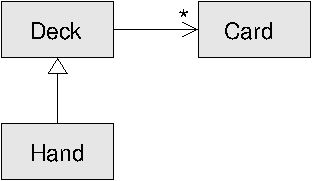
\includegraphics[scale = 0.8] {figs/class1.pdf}}
\caption{Diagrama de Classe.}
\label{} fig.class1
\end{figure}


A seta com uma cabeça oca triângulo representa um IS-A
relação, neste caso indica que herda Mão
do Deck.

A cabeça de seta padrão representa um TEM-A
relação, neste caso um Deck tem referências a cartão
objetos.
\index{multiplicidade (no diagrama de classes)}

A estrela ({\tt *}), perto da cabeça da seta é uma 
{\bf multiplicidade}, que indica quantos cartões um Deck tem.
A multiplicidade pode ser um número simples, como {\tt 52}, um intervalo,
como {\tt 5 .. 7} ou uma estrela, o que indica que um deck pode
ter qualquer número de cartões.

Um diagrama mais detalhado pode mostrar que uma plataforma, na verdade
contém uma {\em lista} of Cards, mas tipos built-in
como lista e dict geralmente não são incluídos nos diagramas de classe.

\begin{} exercício

Leia {\tt TurtleWorld.py}, {\tt World.py} e {\tt Gui.py}
e desenhar um diagrama de classes que mostra as relações entre
as classes definidas lá.

\end{} exercício


\section{} Depuração
\index{depuração}

Herança pode fazer a depuração de um desafio, porque quando você
invocar um método em um objeto, você pode não saber qual o método
será invocado.
\index{polimorfismo}

Suponha que você está escrevendo uma função que funciona com objetos de mão.
Você iria gostar de trabalhar com todos os tipos de mãos, como
PokerHands, BridgeHands, etc Se você chamar um método como
{\tt Shuffle}, você pode obter o que foi definido no {\tt plataforma},
mas se qualquer das subclasses substituir esse método, você vai
obter essa versão em seu lugar.  
\index{fluxo de execução}

Toda vez que você não tem certeza sobre o fluxo de execução através de seu
programa, a solução mais simples é adicionar instruções de impressão no
começando dos métodos relevantes. Se {\tt Deck.shuffle} imprime uma
mensagem que diz algo como {\tt Correndo Deck.shuffle}, então, como
o programa é executado ele traça o fluxo de execução.

Como alternativa, você pode usar esta função, o que leva um
objeto e um nome de método (como uma string) e retorna a classe que
fornece a definição do método:

\begin{verbatim}
def find_defining_class (obj, meth_name):
    para ty em type (obj) MRO ().:
        se meth_name em ty.__dict__:
            retorno ty
\end{verbatim}
%
Aqui está um exemplo:

\begin{verbatim}
>>> Mão = Hand ()
>>> Find_defining_class impressão (lado, shuffle)
<class'Card.Deck'>
\end{verbatim}
%
Assim, o {\tt Shuffle} método para isso é a mão um no {\tt plataforma}.
\{Método mro} índice
\index{método! Mro}
\index{método para resolução}

\Verb "find_defining_class" usa o {\tt mro} método para obter a lista
de objetos de classe (tipos) que será procurado métodos. `` MRO''
significa `` método ordem de resolução.''
\index{override}
\index{Interface}
\index{condição}
\index{pós-condição}

Está aqui um projeto sugestão programa: sempre que você substituir um método,
a interface do novo método deve ser o mesmo que o anterior. Ele
deve ter os mesmos parâmetros, o retorno do mesmo tipo, e obedecer ao
mesmas pré-condições e pós-condições. Se você obedecer a essa regra, você
vai achar que qualquer função projetado para trabalhar com uma instância de uma
superclasse, como um Deck, também irá trabalhar com as instâncias de subclasses
como uma mão ou Pokerhand.

Se você violar esta regra, o código entrará em colapso como (desculpe)
um castelo de cartas.


\section{encapsulamento de dados}

Capítulo ~ \ref {tempo} demonstra um plano de desenvolvimento que podemos chamar
`` Projeto orientado a objetos.'' Nós identificamos objetos que precisávamos --- {\tt
  Tempo}, {\tt Ponto} e {\tt Retângulo} --- e definidas classes para
representá-los. Em cada caso há uma correspondência óbvia
entre o objecto e uma entidade no mundo real (ou pelo menos um
mundo matemático).
\{} Índice plano de desenvolvimento

Mas às vezes é menos óbvio que os objetos que você precisa
e como eles devem interagir. Nesse caso, você precisa de um diferente
plano de desenvolvimento. Da mesma maneira que descobrimos função
as interfaces de encapsulamento e generalização, podemos descobrir
interfaces de classe por {\bf dados encapsulamento}.
\index{encapsulamento de dados}
\index{encapsulamento! Dados}

Análise Markov, da Seção ~ \ref {} Markov, é um bom exemplo.
Se você baixar o meu código de \url{http://thinkpython.com/code/markov.py},
você verá que ele usa duas variáveis ​​globais --- \verbo "suffix_map" e
\Verb "prefixo" --- que são lidos e escritos de diversas funções.

\begin{verbatim}
suffix_map = {}        
prefix = ()            
\end{verbatim}

Como essas variáveis ​​são globais
só podemos executar uma análise
de cada vez. Se lermos dois textos, seus prefixos e sufixos faria
ser adicionados às mesmas estruturas de dados (o que contribui para uma interessante
texto gerado).

Para executar várias análises, e mantê-los separados, podemos encapsular
o estado de cada análise de um objeto.
Aqui está o que parece:

\begin{verbatim}
classe Markov (object):

    def __ init__ (self):
        self.suffix_map = {}
        self.prefix = ()    
\end{verbatim}

Em seguida, vamos transformar as funções em métodos. Por exemplo,
aqui está \verb "process_word":

\begin{verbatim}
    def process_word (self, palavra, order = 2):
        if len (self.prefix) <ordem:
            self.prefix + = (word,)
            retorno

        tente:
            self.suffix_map [self.prefix]. anexar (palavra)
        exceto KeyError:
            # Se não houver nenhuma entrada para esse prefixo, fazer uma
            self.suffix_map [self.prefix] = [palavra]

        self.prefix = shift (self.prefix, word)        
\end{verbatim}

Transformar um programa como este --- alterar o design sem
alterar a função --- é outro exemplo de refatoração
(Ver Seção ~ \ref {refactoring}).
\index{} refatoração

Este exemplo sugere um plano de desenvolvimento para a criação de objetos e
métodos:

\begin{enumerate}

\item Comece por funções que ler escrever e escrever mundial
variáveis ​​(quando necessário).

\item Depois de conseguir o funcionamento do programa, procurar associações
entre as variáveis ​​globais e as funções que os utilizam.

\variáveis ​​Encapsulate item relacionado como atributos de um objeto.

\item Transformar as funções associadas a métodos do novo
classe.

\end{enumerate}


\begin{} exercício

Baixe o meu código da Seção ~ \ref {} Markov
(\url{http://thinkpython.com/code/markov.py}), e siga os passos descritos
acima para encapsular as variáveis ​​globais como atributos de uma nova classe
chamado {\tt Markov}. Solução: \url{http://thinkpython.com/code/Markov.py}
(Nota a capital M).

\end{} exercício




\section{} Glossário

\begin{description}

\item[codificar:] Para representar um conjunto de valores usando outro
conjunto de valores por meio da construção de um mapeamento entre eles.
\index{} codificar

\item[atributo de classe:] Um atributo associado a uma classe
objeto. Atributos de classe são definidos dentro
uma definição de classe, mas fora de qualquer método.
\{Atributo da classe} índice
\index{atributo! Classe}

\[Atributo exemplo:] Item Um atributo associado a um
instância de uma classe.
\index{atributo instance}
\index{atributo! Instance}

\item[verniz:] Um método ou função que fornece uma diferente
interface para outra função sem fazer muito cálculo.
\index{verniz}

\item[herança] A capacidade de definir uma nova classe que é um
versão modificada de uma classe definida anteriormente.
\index{herança}

\item[classe pai:] A classe da qual uma classe filha herda.
\index{classe pai}

\item[class filho:] Uma nova classe criada herdando a partir de um
classe existente; também chamado de `` subclasse''.
\index{classe filha}
\index{classe! Criança}

\item[IS-A relação:] A relação entre uma classe filha
e sua classe pai.
\index{IS-A relação}

\item[TEM-A relação:] A relação entre duas classes
onde as instâncias de uma classe conter referências a casos de
o outro.
\index{TEM-A relação}

\[Diagrama de classes:] item de um diagrama que mostra as classes em um programa
e as relações entre eles.
\{} Diagrama de classes do índice
\index{diagrama! Classe}

\item[multiplicidade:] A notação em um diagrama de classes que mostra, por
A tem-A relação, quantas referências existem para casos
de outra classe.
\index{multiplicidade (no diagrama de classes)}

\end{description}


\section{Exercícios}

\begin{} exercício
\label{} pôquer

A seguir estão as mãos possíveis no poker, em ordem crescente
de valor (e por ordem decrescente de probabilidade):
\index{} pôquer

\begin{description}

\item[par]: duas cartas com o mesmo valor
\Vspace {-0.05in}

\item[dois pares:] dois pares de cartas com o mesmo valor
\Vspace {-0.05in}

\item[três de um tipo:] três cartas com o mesmo valor
\Vspace {-0.05in}

\item[reta]: cinco cartas com fileiras em sequência (As pode
ser alta ou baixa, então {\tt Ace-2-3-4-5} é uma reta e por isso é {\tt
10-Jack-Rainha-Rei-Ace}, mas {\tt Queen-King-Ace-2-3} não é.)
\Vspace {-0.05in}

\item[] Flush: cinco cartas com o mesmo naipe
\Vspace {-0.05in}

\item[full house:] três cartas com mesmo valor, duas cartas com outro
\Vspace {-0.05in}

\item[four of a kind:] quatro cartas com o mesmo valor
\Vspace {-0.05in}

\item[straight flush:] cinco cartas em sequência (como definido acima) e
com o mesmo terno
\Vspace {-0.05in}

\end{description}
%
O objetivo destes exercícios é estimar
a probabilidade de traçar estas várias mãos.

\begin{enumerate}

\item Faça o download dos seguintes arquivos de \url{http://thinkpython.com/code}:

\begin{description}

\item[{\tt Card.py}]: Uma versão completa do {\tt Cartão},
{\tt plataforma} e {mão \tt} classes neste capítulo.

\item[{\tt PokerHand.py}]: Uma implementação incompleta de uma classe
que representa uma mão de poker, e um código que testa-lo.

\end{description}
%
\item Se você executar {\tt PokerHand.py}, trata-se de sete 7-cartão mãos de poker
e verifica se algum deles contém um flush. Leia este
código com cuidado antes de ir em frente.

\item Adicionar métodos para {\tt PokerHand.py} chamado \verb "has_pair",
\Verb "has_twopair", etc, que retornar true ou false de acordo com
se ou não a mão satisfaz os critérios pertinentes. Seu código deve
funcionar corretamente para `` mãos'' que contenham qualquer número de cartões
(Embora 5 e 7 são os tamanhos mais comuns).

\item Escrever um método chamado {\tt classificam} que descobre
a classificação de maior valor para um lado e define o
{Label \tt} atribuir em conformidade. Por exemplo, uma mão de 7 cartas
pode conter um flush e um par, que deve ser escrito `` nivelado.''

\item Quando você está convencido de que os seus métodos de classificação são
de trabalho, o próximo passo é calcular as probabilidades dos diferentes
mãos. Escreva uma função em {\tt PokerHand.py} que embaralha um baralho de
cartões, divide-o em mãos, classifica as mãos, e conta o
número de vezes que várias classificações aparecer.

\item Imprimir uma tabela de classificações e suas probabilidades.
Execute o programa com números cada vez maiores de mãos até que a
valores de saída convergem para um grau razoável de precisão. Comparar
os resultados para os valores em \url{http://en.wikipedia.org/wiki/Hand_rankings}.

\end{enumerate}

Solução: \url{http://thinkpython.com/code/PokerHandSoln.py}.
\end{} exercício


\begin{} exercício
\index{} Swampy
\index{} TurtleWorld

Este exercício usa TurtleWorld do capítulo ~ \ref {} turtlechap.
Você vai escrever um código que faz Turtles tag jogo. Se você
não estão familiarizados com as regras de etiqueta, consulte
\url{http://en.wikipedia.org/wiki/Tag_ (jogo)}.

\begin{enumerate}

\item Download \url{} http://thinkpython.com/code/Wobbler.py e executá-lo. Você
deve ver um TurtleWorld com três tartarugas. Se você pressionar o
Botão {\sf Run}, as Tartarugas vagar a esmo.

\item Leia o código e certifique-se de compreender como ele funciona.
O {\tt Wobbler} classe herda de {\tt Turtle}, o que significa
que as {\tt tartaruga} métodos {\tt lt}, {\tt rt}, {\tt fd}
e {\tt bk} trabalhar em Wobblers.

O passo {\tt} método é invocado por TurtleWorld. Invoca
{\tt boi}, que transforma a tartaruga na direção desejada,
{\tt oscilação}, que faz uma curva aleatória na proporção da tartaruga de
falta de jeito, e {tt move \}, que avança alguns pixels,
dependendo da velocidade da tartaruga.
\index{} Tagger

\item Crie um arquivo chamado {\tt Tagger.py}. Importar tudo, desde
  {\tt Wobbler}, então, definir uma classe chamada {\tt Tagger} que herda
  do {\tt Wobbler}. Chame \verb "make_world" passar o {\tt
    Tagger} objeto de classe como um argumento.

\item Adicionar uma {\tt boi} método para {\tt Tagger} para substituir o de
  {\tt Wobbler}. Como ponto de partida, escreva uma versão que sempre
  aponta a tartaruga para a origem. Dica: use a função matemática
  {\tt atan2} ea tartaruga atributos {\tt x}, {\tt y} e
  {Tt título \}.

\item Modificar {\tt boi} para que as tartarugas ficar em limites.
  Para depuração, você pode querer usar o botão {\sf Passo},
  que invoca {passo \tt} uma vez em cada Turtle.

\item Modificar {\tt boi} de modo que cada ponto da tartaruga em direção a seu mais próximo
  vizinho. Dica: As tartarugas têm um atributo, {mundo \tt}, que é um
  referência ao TurtleWorld em que vivem, e tem TurtleWorld
  um atributo, {\tt animais}, que é uma lista de todas as tartarugas no
  mundo.

\item Modificar {\tt boi} então a tag jogo Turtles. Você pode adicionar métodos
  para {\tt Tagger} e você pode substituir {\tt boi} e
  \Verb "__init__", mas você não pode modificar ou substituir {passo \tt}, {\tt
    oscilação} ou {\tt movimento}. Além disso, {\tt boi} tem permissão para alterar a
  rubrica do Turtle, mas não a posição.

Ajuste as regras e sua {\tt boi} método para o jogo de boa qualidade;
por exemplo, deverá ser possível para a tartaruga lenta para marcar o
Tartarugas mais rápidas, eventualmente.

\end{enumerate}

Solução: \url{http://thinkpython.com/code/Tagger.py}.
\end{} exercício



\chapter{Estudo de caso: Tkinter}
\label{} tkinter

\section{GUI}

A maioria dos programas que temos visto até agora são baseados em texto, mas
muitos programas usam {interfaces gráficas de usuário \bf}, também
conhecido como {\bf GUIs}.
\index{GUI}
\index{interface gráfica do usuário}
\index{} Tkinter

Python fornece várias opções para escrever programas baseados em GUI,
incluindo wxPython, Tkinter, e Qt. Cada um tem prós e contras, o que
É por isso que Python não convergiu em um padrão.

O que eu vai apresentar neste capítulo é Tkinter porque eu acho que
é o mais fácil de começar a usar. A maior parte dos conceitos
neste capítulo aplicam-se aos outros módulos GUI, também.

Existem vários livros e páginas da web sobre Tkinter. Um dos
os melhores recursos on-line é {\em Uma Introdução à Tkinter}
por Fredrik Lundh.
\index{módulo Gui}
\index{módulo! Gui}
\index{} Swampy

Eu escrevi um módulo chamado {\tt Gui.py} que vem com
Swampy. Ele fornece uma interface simplificada para as funções
e as aulas em Tkinter. Os exemplos neste capítulo são
com base nesse módulo.

Aqui está um exemplo simples que cria e exibe uma interface gráfica:

Para criar um GUI, você tem que importar {\tt Gui} de Swampy:
%
\begin{verbatim}
de swampy.Gui import *
\end{verbatim}
%
Ou, dependendo de como você instalou o Swampy, como este:
%
\begin{verbatim}
Gui de importação *
\end{verbatim}
%
Em seguida, instanciar um objeto Gui:
%
\begin{verbatim}
g = Gui ()
g.title ('Gui')
g.mainloop ()
\end{verbatim}
%
Ao executar este código, uma janela deve aparecer com um cinza vazio
quadrado eo título {\sf Gui}. {\tt mainloop} corre o evento {\bf
  laço}, que espera que o usuário de fazer alguma coisa e responde
em conformidade. É um ciclo infinito, que vai até o usuário fechar
da janela, ou pressionar Control-C, ou faz algo que faz com que o
programa para parar de fumar.
\index{ciclo de eventos}
\index{laço! Evento}
\index{loop infinito}
\index{laço! Infinito}

A presente Gui não muito, porque ele não tem qualquer
{\bf Widgets}. Widgets são os elementos que compõem um
GUI, que incluem:
\index{} Widget

\begin{description}

\item[Button:] Um widget, com o texto ou uma imagem, que
executa uma ação quando pressionado.

\item[Canvas:] Uma região que pode exibir linhas, retângulos,
círculos e outras formas.

\item[Entrada:] A região onde os usuários podem digitar texto.

\item[Barra de rolagem:] Um widget que controla a parte visível de um outro
widget.

\item[Quadro]: Um recipiente, muitas vezes invisível, que contém outros
widgets.

\end{description}

O quadrado cinza vazio que você vê quando você cria um Gui é
um Frame. Quando você cria um novo widget, ele é adicionado a este quadro.



\section{Botões e retornos de chamada}
\index{Widget Botão}
\index{widget! Botão}

O método {\tt bu} cria um widget Button:

\begin{verbatim}
botão = g.bu (text = 'Prima me.')
\end{verbatim}
%
O valor de retorno {\tt bu} é um objeto Button. O botão
que aparece no quadro é uma representação gráfica deste
objeto, você pode controlar o botão invocando métodos sobre ele.
\index{opção}

{\tt bu} leva até 32 parâmetros que controlam a aparência
e função do botão. Estes parâmetros são chamados
{options \bf}. Em vez de fornecer valores para todas as 32 opções,
você pode usar argumentos, como \verb "text = 'Imprensa mim.'",
para especificar apenas as opções que você precisa e usar o padrão
Os valores para o resto.
\index{argumento palavra-chave}
\index{argumento! Keyword}

Quando você adicionar um widget para o quadro, torna-se `` devidamente embalados;''
isto é, o Quadro encolhe com o tamanho do botão. Se você
adicionar mais widgets, o quadro cresce para acomodá-los.
\index{Widget Etiqueta}
\index{widget! Etiqueta}

O método {\tt la} cria um widget Etiqueta:

\begin{verbatim}
label = g.la (text = "Pressione o botão. ')
\end{verbatim}
%
Por padrão, o Tkinter empilha os widgets de cima para baixo e centros
los. Vamos ver como substituir esse comportamento em breve.

Se você pressionar o botão, você vai ver que ele não faz muita coisa.
Isso é porque você não tem `` com fio-o;'' ou seja, você não tem
lhe diga o que fazer!

A opção que controla o comportamento de um botão é {comando \tt}.
O valor de {comando \tt} é uma função que é executada quando
o botão é pressionado. Por exemplo, aqui está uma função que cria
um novo rótulo:

\begin{verbatim}
def make_label ():
    g.la (text = 'Obrigado.')
\end{verbatim}
%
Agora podemos criar um botão com essa função como seu comando:

\begin{verbatim}
button2 = g.bu (text = 'Não, pressionar-me!', command = make_label)
\end{verbatim}
%
Ao pressionar este botão, ele deve executar \verb "make_label"
e um novo rótulo deve aparecer.
\index{callback}

O valor da opção {comando \tt}
é um objeto de função, que é conhecido como um callback {\bf} porque
depois que você chamar {\tt bu} para criar o botão, o fluxo de execução
`` Chama de volta'' quando o usuário pressiona o botão.
\index{programação orientada a eventos}

Este tipo de fluxo é característico de {programação orientada a eventos \bf}.
As ações do usuário, como prensas de botões e comandos de teclado, são chamados de {\bf
eventos}. Na programação orientada a eventos, o fluxo de execução é
determinado pela acção do utilizador, em vez de pelo programador.  

O desafio de programação orientada a eventos é a construção de um conjunto de
widgets e callbacks que trabalham corretamente (ou pelo menos geram
mensagens de erro apropriadas) para qualquer seqüência de ações do usuário.

\begin{} exercício

Escreva um programa que cria uma interface gráfica com um único botão. Quando o
botão é pressionado ele deve criar um segundo botão. Quando
{\Em que} botão é pressionado, ele deve criar um rótulo que
diz: `` Bom trabalho!''.

O que acontece se você pressionar os botões mais de uma vez?
Solução: \url{http://thinkpython.com/code/button_demo.py}

\end{} exercício


\section{Widgets lona}
\index{Widget Canvas}
\index{widget! Canvas}

Um dos elementos mais versáteis é a tela, o que cria
uma região para desenhar linhas, círculos e outras formas. Se você
fez Exercício ~ \ref {} tela você já está familiarizado com telas.

O método {\tt ca} cria um novo Canvas:

\begin{verbatim}
tela = g.ca (width = 500, height = 500)
\end{verbatim}
%
{Width \tt} e {height \tt} são as dimensões da tela
em pixels.  
\{Método de configuração} índice
\index{método! Configuração}

Depois de criar um widget, você ainda pode alterar os valores de
as opções com o
{Config \tt} método. Por exemplo, o {\tt bg} alterações de opção
a cor de fundo:

\begin{verbatim}
canvas.config (bg = 'branco')
\end{verbatim}
%
O valor de {\tt bg} é uma seqüência
que os nomes de uma cor. O conjunto de nomes de cores legais é diferente
para diferentes implementações de Python, mas todas as implementações
fornecer, pelo menos:

\begin{verbatim}
preto branco
azul verde vermelho   
cyan magenta amarelo
\end{verbatim}
%
Shapes em um Canvas são chamados itens {\bf}. Por exemplo,
o método Canvas {círculo \tt} chama (você adivinhou) um círculo:
\index{item de lona}
{Canvas artigo!} \Index

\begin{verbatim}
artigo = canvas.circle ([0,0], 100, fill = 'red')
\end{verbatim}
%
O primeiro argumento é um par de coordenadas que especifica a
centro do círculo, o segundo é o raio.
\index{Canvas coordenar}
{Canvas coordenar!} \Index

{\tt Gui.py} fornece um sistema de coordenadas cartesianas padrão com
a origem no centro da tela e os US $ positivo y $ eixo
apontando para cima. Isto é diferente de alguns outros sistemas gráficos
em que a origem é, no canto superior esquerdo, com o eixo y $ $
apontando para baixo.

A opção {\tt preenchimento} especifica que o círculo deve ser preenchido
com vermelho.

O valor de retorno {\tt círculo} é um objeto do item que
fornece métodos para a modificação do item na tela. Para
exemplo, você pode usar {config \tt} para alterar qualquer do círculo de
opções:

\begin{verbatim}
item.config (preencher = 'amarelo', esboço = 'laranja', width = 10)
\end{verbatim}
%
{Width \tt} é a espessura do contorno em pixels;
{Esboço \tt} é a cor.

\begin{} exercício
\label{círculo}

Escreva um programa que cria uma lona e um Button. Quando o
usuário pressiona o botão, ele deve desenhar um círculo na tela.

\end{} exercício


\section{Coordenar seqüências}
\index{coordenar seqüência}
\index{seqüência! Coordenar}

O {\tt retângulo} método leva uma seqüência de coordenadas que
especificar cantos opostos do retângulo. Este exemplo
desenha um retângulo verde com o canto inferior esquerdo na origem
e no canto superior direito em US $ (200.100) $:

\begin{verbatim}
canvas.rectangle ([[0, 0], [200, 100]], 
                 preencher = 'blue', esboço = 'laranja', width = 10)
\end{verbatim}
%
Esta forma de cantos especificando é chamado
uma caixa {\bf delimitadora} porque os dois pontos
obrigado retângulo.
\index{caixa delimitadora}

{\tt oval} tem uma caixa delimitadora e desenha uma oval
dentro do retângulo especificado:

\begin{verbatim}
canvas.oval ([[0, 0], [200, 100]], esboço = 'laranja', width = 10)
\end{verbatim}
%
{Line \tt} leva uma seqüência de coordenadas e desenha
uma linha que liga os pontos. Este exemplo desenha duas pernas
de um triângulo:

\begin{verbatim}
canvas.line ([[0, 100], [100, 200], [200, 100]], largura = 10)
\end{verbatim}
%
{\tt polígono} leva os mesmos argumentos, mas ele desenha o último
perna do polígono (se necessário) e enche-lo em:

\begin{verbatim}
canvas.polygon ([[0, 100], [100, 200], [200, 100]],
               preencher = 'vermelho', esboço = 'laranja', width = 10)
\end{verbatim}
%


\section{} mais widgets
\index{widget de texto}
\index{widget! Texto}

Tkinter fornece dois widgets que permitem aos usuários o tipo de texto: um
Entrada, que é uma única linha, e um widget de texto, que tem
várias linhas.
\index{Widget entrada}
\index{widget! Entry}

{\tt en} cria uma nova entrada:

\begin{verbatim}
entry = g.en (text = 'text padrão.')
\end{verbatim}
%
A {text \tt} opção permite que você coloque o texto na entrada
quando ele é criado. O {get \tt} método retorna o conteúdo
da entrada (que pode ter sido alterado pelo usuário):

\begin{verbatim}
>>> Entry.get ()
'Texto padrão.
\end{verbatim}
%
{\tt te} cria um widget de texto:

\begin{verbatim}
text = g.te (width = 100, height = 5)
\end{verbatim}
%
{Width tt \} e {height \tt} são as dimensões do
Widget em personagens e linhas.

{Inserir \tt} coloca texto na janela de texto:

\begin{verbatim}
text.insert (END, 'A linha de texto.')
\end{verbatim}
%
{\tt END} é um índice especial que indica o último caractere na
Widget de Texto.

Você também pode especificar um caractere usando um índice pontilhada, como {\tt 1.1},
que tem o número de linha antes do ponto e o número da coluna depois.
O exemplo a seguir adiciona as letras \verb "'nother" após a primeira
caractere da primeira linha.

\begin{verbatim}
>>> Text.insert (1,1, 'utro')
\end{verbatim}
%
O {get \tt} método lê o texto no widget, leva um começo
eo índice final como argumentos. O exemplo a seguir retorna todos os
texto no widget, incluindo o caractere de nova linha:

\begin{verbatim}
>>> Text.get (0.0, END)
"Outra linha de texto. \N '
\end{verbatim}
%
O {\tt apagar} método remove texto do widget;
exemplo a seguir exclui todos, mas os dois primeiros caracteres:

\begin{verbatim}
>>> Text.delete (1.2, END)
>>> Text.get (0.0, END)
'Um \n'
\end{verbatim}
%

\begin{} exercício
\label{} circle2

Modifique a sua solução para o Exercício ~ \ref {} círculo, adicionando um
Widget de entrada e um segundo botão. Quando o usuário pressiona a
segundo botão, ele deve ler um nome de cor a partir da entrada e
usá-lo para mudar a cor de preenchimento do círculo. Use {config \tt}
para modificar o círculo existente, não criar um novo.

Seu programa deve tratar o caso em que o usuário tenta
mudar a cor de um círculo que não tenha sido criado, e
o caso em que o nome da cor é inválida.

Você pode ver a minha solução em \url{http://thinkpython.com/code/circle_demo.py}.

\end{} exercício


\section{Embalagem Widgets}

Até agora, temos sido empilhamento widgets em uma única coluna, mas na maioria
GUIs o layout é mais complicada. Por exemplo,
Figura ~ \ref {fig.turtleworld} mostra uma versão simplificada do
TurtleWorld (ver capítulo ~ \ref {turtlechap}).

\begin{figure}
\Ce nterline {\includegraphics[scale = 0.5] {figos / TurtleWorld.pdf}}
\caption{Diagrama de Classe.}
\label{} fig.turtleworld
\end{figure}


Esta seção apresenta o código que cria essa GUI, quebrado em um
série de passos. Você pode baixar o exemplo completo
de \url{http://thinkpython.com/code/SimpleTurtleWorld.py}.

No nível superior, este GUI contém dois widgets --- uma lona e uma
Quadro --- dispostas em uma fileira. Assim, a primeira etapa é a de criar a linha.
\index{classe SimpleTurtleWorld}
\{SimpleTurtleWorld classe!} Índice

\begin{verbatim}
classe SimpleTurtleWorld (TurtleWorld):
    "" "Esta classe é idêntica à TurtleWorld, mas o código que
    estabelece a GUI é simplificada para fins explicativos. "" "

    configuração def (self):
        self.row ()
        ...
\end{verbatim}
%
{Setup \tt} é a função que cria e organiza os widgets.
Organizando widgets em uma GUI é chamado {\bf embalagem}.
\index{Widgets embalagem}
\index{widget, embalagem}
\index{Widget Quadro}
\index{widget! Quadro}

{\tt linha} cria um quadro de linha e torna o `` quadro atual.''
Até este quadro é fechado ou outro quadro é criado, tudo
Widgets subseqüentes são embalados em uma fileira.

Aqui está o código que cria a tela ea moldura coluna
que detêm os outros widgets:

\begin{verbatim}
        self.canvas = self.ca (width = 400, height = 400, bg = 'branco')
        self.col ()
\end{verbatim}
%
O primeiro widget na coluna é uma estrutura de grade, que contém
quatro botões dispostos dois a dois:

\begin{verbatim}
        self.gr (cols = 2)
        self.bu (text = "tela Print ', command = self.canvas.dump)
        self.bu (text = 'Sair', command = self.quit)
        self.bu (text = 'Make Turtle', command = self.make_turtle)
        self.bu (text = 'Clear', command = self.clear)
        self.endgr ()
\end{verbatim}
%
{\tt gr} cria a grade, o argumento é o número de
colunas. Widgets na grade são
colocado para fora da esquerda para a direita, de cima para baixo.
\index{callback}
\index{método obrigado}
\index{método, com destino}
\index{assunto}

O primeiro botão usos {\tt self.canvas.dump} como uma chamada de retorno, o segundo
usos {\tt self.quit}. Estes são métodos {\bf encadernados}, que significa
estão associados com um determinado objecto. Quando eles são invocados, eles
são invocados no objeto.

A próxima widget na coluna é um quadro linha que contém
um botão e uma entrada:

\begin{verbatim}
        self.row ([0,1], pady = 30)
        self.bu (text = 'file funcionar ", command = self.run_file)
        self.en_file = self.en (text = 'snowflake.py', width = 5)
        self.endrow ()
\end{verbatim}
%
O primeiro argumento para {\tt linha} é uma lista de pesos que
determina como espaço extra é alocada entre widgets.  
A lista {\tt [0,1]} significa que todo o espaço extra é alocada
para o segundo widget, que é a entrada. Se você executar esse código
e redimensionar a janela, você vai ver que a entrada cresce e
o botão não.

A opção {\tt pady} `` blocos'' esta linha no $ $ y direção,
adição de 30 pixels de espaço acima e abaixo.

{\tt EndRow} termina esta linha de widgets, widgets para posteriores são
embalado no Quadro coluna. {\tt Gui.py} mantém uma pilha de quadros:

\begin{itemize}

\item Quando você usa {linha \tt}, {\tt col} ou {\tt gr} para criar um quadro,
vai para o topo da pilha e se torna o quadro atual.

\item Quando você usa {\tt EndRow}, {\tt ColFinal} ou {\tt endgr} para fechar
um quadro, ele é retirado da pilha e do quadro anterior na
pilha torna-se o quadro atual.

\end{itemize} 

O método \verb "run_file" lê o conteúdo da entrada,
usa-lo como um nome de arquivo, lê o conteúdo
e passa a \verbo "run_code". {\tt self.inter} é um
Objeto intérprete que sabe como levar uma corda e
executá-lo como código Python.

\begin{verbatim}
    run_file def (self):
        filename = self.en_file.get ()
        fp = open (filename)
        source = fp.read ()
        self.inter.run_code (fonte, nome do arquivo)
\end{verbatim}
%
Os dois últimos elementos são um widget de texto e um botão:

\begin{verbatim}
        self.te_code self.te = (largura = 25, altura = 10)
        self.te_code.insert (END ', world.clear () \n')
        self.te_code.insert (END, 'bob = Turtle (mundo) \n')

        self.bu (text = 'Código de funcionar ", command = self.run_text)
\end{verbatim}
%
\Verb "run_text" é semelhante ao verbo \"run_file" exceto que ele leva
o código do widget de texto em vez de um arquivo:

\begin{verbatim}
    run_text def (self):
        source = self.te_code.get (1.0, END)
        self.inter.run_code (fonte: 'code> <user-provided')
\end{verbatim}
%
Infelizmente, os detalhes do esquema são diferentes na ferramenta
outros idiomas, e em diferentes módulos Python.
Tkinter sozinho fornece três diferentes mecanismos para organizar
widgets. Estes mecanismos são chamados de gerentes de geometria {\bf}.
O que eu demonstrado nesta seção é a geometria grade ``''
gerente, os outros são chamados de `` pacote'' e `` local''.
\index{gerenciador de geometria}

Felizmente, a maioria dos conceitos nesta seção aplicam-se a
outros módulos GUI e outras línguas.


\section{Menus e Callables}
\index{Widget MENUBUTTON}
\index{widget! MENUBUTTON}

A MENUBUTTON é um widget que se parece com um botão, mas quando pressionado
ele aparece um menu. Depois que o usuário seleciona um item, o menu
desaparece.

Aqui está o código que cria uma seleção de cores MENUBUTTON
(Você pode baixá-lo a partir de \url{http://thinkpython.com/code/menubutton_demo.py}):

\begin{verbatim}
g = Gui ()
g.la ('Selecione uma cor:')
cores = ['vermelho', 'verde', 'blue']
mb = g.mb (text = cores [0])
\end{verbatim}
%
{\tt mb} cria a MENUBUTTON. Inicialmente, o texto no botão é
o nome da cor padrão. O circuito a seguir cria um menu de
item para cada cor:

\begin{verbatim}
para a cor nas cores:
    G.MI (mb, text = cor, command = mobilizável (set_color, cor))
\end{verbatim}
%
O primeiro argumento de {\tt mi} é o MENUBUTTON esses itens são
associado.
\index{callback}
\index{objeto mobilizável}
\index{objeto! Mobilizável}

A opção {comando \tt} é um objeto mobilizável, que é algo novo.
Até agora, temos funções e métodos vinculados usados ​​como callbacks visto,
que funciona bem se você não tem que passar quaisquer argumentos para
a função. Caso contrário, você tem que construir um objeto mobilizável
que contém uma função, como \verb "set_color", e seus argumentos,
como {\tt color}.

O objeto mobilizável armazena uma referência para a função e o
argumentos como atributos. Mais tarde, quando o usuário clica em um menu
item, o callback chama a função e passa o armazenados
argumentos.

Aqui está o que \verb "set_color" pode parecer:

\begin{verbatim}
set_color def (cor):
    mb.config (text = cor)
    cor de impressão
\end{verbatim}
%
Quando o usuário seleciona um item de menu e \verb "set_color" é chamado,
ele configura o MENUBUTTON para exibir a cor recém-selecionada.
Ele também imprimir a cor, se você tentar este exemplo, é possível confirmar que
\Verb "set_color" é chamado quando você selecionar um item (e {\em não}
chamado quando você cria o objeto mobilizável).


\section{Binding}
\index{ligação}
\index{callback}

A {\bf} ligação é uma associação entre um widget, um evento e um
callback: quando um evento (como um botão de imprensa) acontece em um widget, o
callback é invocado.

Muitos elementos têm ligações padrão. Por exemplo, quando você pressiona
um botão, a ligação padrão muda o alívio do botão
para torná-la deprimida. Quando você soltar o botão, o
ligação restaura a aparência do botão e invoca o
callback especificado com a opção {comando \tt}.

Você pode usar o {\tt ligam} método para substituir estes default
ligações ou para adicionar novos. Por exemplo, este código cria uma
vinculativo para uma tela (você pode baixar o código deste
seção de \url{http://thinkpython.com/code/draggable_demo.py}):

\begin{verbatim}
ca.bind ('<ButtonPress-1>', make_circle)
\end{verbatim}
%
O primeiro argumento é uma cadeia de eventos, o evento é acionado
quando o usuário pressiona o botão esquerdo do mouse. Outro rato
eventos incluem {\tt ButtonMotion}, {\tt ButtonRelease} e
{\tt duas vezes botão}.
\index{string evento}
\index{manipulador de eventos}

O segundo argumento é um manipulador de eventos. Um manipulador de eventos
é uma função ou método vinculado, como um retorno de chamada, mas um importante
diferença é que um manipulador de eventos recebe um objeto de evento como um
parâmetro. Aqui está um exemplo:

\begin{verbatim}
def make_circle (evento):
    pos = ca.canvas_coords ([event.x, event.y])
    artigo = ca.circle (pos, 5, preencher = 'red')
\end{verbatim}
%
O objeto de evento contém informações sobre o tipo de evento e
detalhes como as coordenadas do ponteiro do mouse. Neste exemplo
as informações que precisamos é
a localização do clique do mouse. Estes
Os valores estão em `` coordenadas de pixel'', que são definidos pela
sistema gráfico subjacente. Os método \verb "canvas_coords"
os traduz para `` coordenadas em Canvas,'' que são compatíveis com
Métodos de lona como {\tt círculo}.
\index{objeto Event}
\index{objeto! Evento}

Para os itens de entrada, é comum para ligar a \verb "<Return>" evento,
que é acionado quando o usuário pressiona a {\sf retorno} ou
{\Sf Enter}. Por exemplo, o código a seguir cria um botão
e uma entrada.

\begin{verbatim}
bu = g.bu ('Faça item de texto:', make_text)
en = g.en ()
en.bind ('<Return>', make_text)
\end{verbatim}
%
\Verb "make_text" é chamado quando o botão for pressionado ou quando
o usuário clica em {\sf retorno} durante a digitação na entrada. Para fazer
Neste trabalho, nós precisamos de uma função que pode ser chamado como um comando
(Sem argumentos) ou como um manipulador de eventos (com um evento
como um argumento):

\begin{verbatim}
def make_text (event = None):
    text = en.get ()
    artigo = ca.text ([0,0], texto)
\end{verbatim}
%
\Verb "make_text" recebe o conteúdo da entrada e exibe
lo como um item de texto na tela.

Também é possível criar ligações para Artigos de lona.
O seguinte é uma definição de classe para {\tt Draggable},
que é uma classe filha de {\tt item} que fornece ligações
que implementam a capacidade de arrastar-e-soltar.
\index{drag-and-drop}

\begin{verbatim}
classe Draggable (Item):

    def __ init__ (self, item):
        self.canvas = item.canvas
        self.tag = item.tag
        self.bind ('<Button-3>', self.select)
        self.bind ('<B3-Motion>', self.drag)
        self.bind ('<Release-3>', self.drop)
\end{verbatim}
%
O método init leva um item como um parâmetro. Ele copia
os atributos do item e, em seguida, cria ligações para
três eventos: a imprensa, botão de movimento, e solte o botão.

O manipulador de eventos {\selecionar tt} armazena as coordenadas
do evento atual e a cor original do item, em seguida,
muda a cor para amarelo:

\begin{verbatim}
    def selecionar (self, event):
        self.dragx = event.x
        self.dragy = event.y

        self.fill = self.cget ('preenchimento')
        self.config (preencher = 'amarelo')
\end{verbatim}
%
{\tt CGET} significa `` obter configuração;'' que leva o nome de um
opção como uma seqüência e retorna o valor atual dessa opção.

{\tt arrastar} calcula a distância que o objeto se moveu em relação ao
começando lugar, atualiza as coordenadas armazenados e, em seguida, move o
item.
\index{update! Coordenar}

\begin{verbatim}
    arrastar def (self, event):
        dx = event.x - self.dragx
        dy = event.y - self.dragy

        self.dragx = event.x
        self.dragy = event.y

        self.move (dx, dy)
\end{verbatim}
%
Este cálculo é feito em coordenadas de pixel, não há necessidade de
converter em coordenadas de lona.
\index{Canvas coordenar}
{Canvas coordenar!} \Index
\index{coordenada de pixel}
\index{coordenar! Pixels}

Finalmente, {queda \tt} restaura a cor original do artigo:

\begin{verbatim}
    def cair (self, event):
        self.config (preencher = self.fill)
\end{verbatim}
%
Você pode usar o {\tt Draggable} class para adicionar drag-and-drop
capacidade de um item existente. Por exemplo, aqui está uma modificação
versão do \verb "make_circle" que utiliza {\tt círculo} para criar
um item e {\tt Draggable} para torná-lo arrastado:

\begin{verbatim}
def make_circle (evento):
    pos = ca.canvas_coords ([event.x, event.y])
    artigo = ca.circle (pos, 5, preencher = 'red')
    artigo = Draggable (item)
\end{verbatim}
%
Este exemplo demonstra um dos benefícios da herança: você pode
modificar as capacidades de uma classe pai, sem modificar sua
definição. Isso é particularmente útil se você deseja alterar
comportamento definido em um módulo que não escreveu.


\section{} Depuração
\index{depuração}

Um dos desafios de programação GUI é manter o controle de
que as coisas acontecem quando a GUI está sendo construído e que
as coisas acontecem mais tarde, em resposta a eventos do usuário.
\index{callback}

Por exemplo, quando você estiver configurando um callback, é um erro comum
para chamar a função em vez de passar uma referência a ele:

\begin{verbatim}
def the_callback ():
    print 'Chamado'.

g.bu (text = "Isto é errado! ', command = the_callback ())
\end{verbatim}
%
Se você executar esse código, você vai ver que ele chama de \verb "the_callback"
imediatamente, e {\em seguida} cria o botão. Quando você pressiona o
botão, ele não faz nada, porque o valor de retorno de 
\Verb "the_callback" é {\tt Nenhum}.
Normalmente você não deseja chamar um callback quando você estiver
configuração do GUI, que só deve ser invocada mais tarde, em resposta a
um evento de usuário.
\index{fluxo de execução}
\index{programação orientada a eventos}

Outro desafio de programação GUI é que você não tem controle
do fluxo de execução. Quais as partes do programa de executar
e sua ordem são determinados por ações do usuário.
Isso significa que você tem que projetar o seu programa funcione corretamente
para qualquer sequência possível de eventos.

Por exemplo, o GUI no Exercício ~ \ref {} circle2 tem dois widgets:
cria-se um item de círculo e o outro muda a cor do
Circle. Se o usuário cria o círculo e, em seguida, muda de cor,
não há nenhum problema. Mas e se o usuário altera a cor do
um círculo que ainda não existe? Ou cria mais de um círculo?

Como o número de widgets cresce, é cada vez mais difícil
imagine todas as sequências possíveis de eventos. Uma forma de gerir este
complexidade é para encapsular o estado do sistema em um objeto
e, em seguida, considerar:

\begin{itemize}

\item Quais são os possíveis estados? No exemplo do círculo, nós
pode considerar dois estados: antes e depois que o usuário cria a
primeiro círculo.

\item Em cada estado, os eventos que podem ocorrer? No exemplo,
o usuário pode pressionar um dos botões, ou sair.

\item Para cada par estado-evento, que é o resultado desejado?
Uma vez que existem dois estados e dois botões, há quatro
pares estado-evento a considerar.

\item O que pode causar uma transição de um estado para outro?
Neste caso, existe uma transição quando o utilizador cria
o primeiro círculo.

\end{itemize}

Você também pode achar que é útil para definir e verificar, invariantes que
deve realizar, independentemente da seqüência de eventos.
\index{} invariante

Essa abordagem de programação GUI pode ajudá-lo a escrever correto
código sem tomar o tempo para testar cada seqüência possível
de eventos do usuário!


\section{} Glossário

\begin{description}

\item[GUI:] A interface gráfica do usuário.
\index{GUI}

\item[widget:] Um dos elementos que compõem uma interface gráfica, incluindo
botões, menus, campos de entrada de texto, etc 
\index{} Widget

\item[opção:] Um valor que controla a aparência ou a função de
um widget.
\index{opção}

\item[argumento palavra-chave:] Um argumento que indica o parâmetro
nomear como parte da chamada de função.
\index{argumento palavra-chave}

\item[callback]: A função associada a um widget que é
chamada quando o usuário executa uma ação.
\index{callback}

\item[método obrigado:] Um método associado a uma instância particular.
\index{método obrigado}

\item[programação orientada a eventos:] Um estilo de programação no qual
o fluxo de execução é determinado por ações do usuário.
\index{programação orientada a eventos}

\item[evento]: A ação do usuário, como um clique do mouse ou pressione a tecla, que
provoca uma GUI para responder.
\index{evento}

\item[ciclo de eventos:] um loop infinito que espera por ações do usuário
e responde.
\index{ciclo de eventos}

\item[Item]: um elemento gráfico em um widget Canvas.
{Canvas artigo!} \Index

\item[delimitadora caixa:] Um retângulo que inclui um conjunto de itens,
geralmente especificado por dois cantos opostos.
\index{caixa delimitadora}

\item[pacote]: Para organizar e exibir os elementos de uma GUI.
\index{Widgets embalagem}

\item[gerente de geometria:] Um sistema para widgets de embalagem.
\index{gerenciador de geometria}

\item[ligação]: uma associação entre um widget, um evento, e
um manipulador de eventos. O manipulador de eventos é chamado quando o evento
ocorre no widget.
\index{ligação}

\end{description}


\section{Exercícios}

\begin{} exercício
\index{visualizador de imagens}

Para este exercício, você vai escrever um visualizador de imagens. Aqui está
um exemplo simples:

\begin{verbatim}
g = Gui ()
tela = g.ca (width = 300)
foto = PhotoImage (file = 'danger.gif')
canvas.image ([0,0], image = foto)
g.mainloop ()
\end{verbatim}
%
{\tt PhotoImage} lê um arquivo e retorna um {\tt PhotoImage} objeto
Tkinter que pode exibir. {\tt Canvas.image} coloca a imagem na
tela, centrado nas coordenadas dadas. Você também pode colocar as imagens em
etiquetas, botões e alguns outros widgets:

\begin{verbatim}
g.la (image = foto)
g.bu (image = foto)
\end{verbatim}
%
PhotoImage só pode lidar com alguns formatos de imagem, como GIF e PPM, 
mas podemos usar o Python Imaging Library (PIL) para ler outro
arquivos.
\index{Python Imaging Library (PIL)}
\index{PIL (Python Imaging Library)}
\index{módulo Imagem}
\index{módulo! Imagem}

O nome do módulo PIL é {\tt Imagem}, mas Tkinter define um
objeto com o mesmo nome. Para evitar o conflito, você pode usar {\tt
  import ...} como assim:

\begin{verbatim}
importação imagem como PIL
ImageTk importação
\end{verbatim}
%
As importações de primeira linha {\tt imagem} e
lhe dá o nome local {\tt PIL}. A segunda
importações de linha {\tt ImageTk}, o que pode traduzir uma PIL
imagem em um Tkinter PhotoImage. Aqui está um exemplo:

\begin{verbatim}
image = PIL.open ('allen.png')
photo2 = ImageTk.PhotoImage (imagem)
g.la (image = foto2)
\end{verbatim}
%

\begin{enumerate}

\item Download \verbo "image_demo.py", \verb "danger.gif" e \verb "allen.png"
de \url{http://thinkpython.com/code}. Execute \verb "image_demo.py". Você
pode ter que instalar {\tt PIL} e {\tt ImageTk}.  
Eles são, provavelmente, em seu repositório de software, mas se não
você pode obtê-los a partir de \url{pythonware.com / produtos / pil /}.

\item Em \verb "image_demo.py" mudar o nome do segundo
PhotoImage de {\tt photo2} para {\tt foto} e execute o programa
novamente. Você deverá ver o segundo PhotoImage, mas não o primeiro.

O problema é que quando você transferir {\tt foto} ele substitui
a referência à primeira PhotoImage, que, em seguida, desaparece. O
mesma coisa acontece se você atribuir um PhotoImage a um local de
variável, que desaparece quando a função termina.

Para evitar esse problema, você tem que armazenar uma referência para cada
PhotoImage você deseja manter. Você pode usar uma variável global, ou
loja PhotoImages em uma estrutura de dados ou como um atributo de
um objeto.

Este comportamento pode ser frustrante, e é por isso que estou alertando
você (e por que a imagem de exemplo diz `` Perigo!'').
\index{bug! Pior}
\index{pior bug! Nunca}

\item A partir deste exemplo, escrever um programa que leva
o nome de um diretório e percorre todos os arquivos, exibindo
todos os arquivos que PIL reconhece como imagens. Você pode usar um {\tt tentativa}
declaração para pegar os arquivos não PIL não reconhece.

Quando o usuário clica na imagem, o programa deve exibir o próximo.

\item PIL oferece uma variedade de métodos para manipular imagens.
Você pode ler sobre eles em \url{http://pythonware.com/library/pil/handbook}.
Como desafio, escolher alguns destes métodos e fornecer um
GUI para aplicá-los às imagens.

\end{enumerate}

Solução: \url{http://thinkpython.com/code/ImageBrowser.py}.

\end{} exercício


\begin{} exercício
\{} Gráficos vetoriais índice
\index{} SVG

Um editor de gráficos vetoriais é um programa que permite aos usuários desenhar e
editar formas na tela e gerar arquivos de saída em gráficos vetoriais
formatos como Postscript e SVG.

Escrever um editor de gráficos vetoriais simples usando Tkinter. Numa
mínimo, deve permitir que os usuários para desenhar linhas, círculos e
retângulos, e ele deve usar {\tt Canvas.dump} para
gerar uma descrição Postscript dos conteúdos do
Canvas.

Como um desafio, você pode permitir que os usuários selecionem e redimensionar
itens na tela.

TODO: escrever uma solução!

\end{} exercício


\begin{} exercício

Use Tkinter para escrever um navegador básico. Ele
deve ter um widget de texto onde o usuário pode digitar uma URL
e uma tela para exibir o conteúdo da página.
\index{módulo urllib}
\index{módulo! Urllib}
\index{URL}
\index{módulo HTMLParser}
\index{módulo! HTMLParser}

Você pode usar o {\tt urllib} módulo para download de arquivos
(Ver Exercício ~ \ref {urllib}) e
o {\tt HTMLParser} módulo para analisar o HTML
etiquetas (ver \url{http://docs.python.org/2/library/htmlparser.html}).
\index{text plain}
\index{text! Plain}
\index{} hyperlink

No mínimo o navegador deve lidar com texto simples e hyperlinks. Como
um desafio que você poderia lidar com as cores de fundo, texto
tags de formatação e imagens.

TODO: escrever uma solução!

\end{} exercício



\appendix

\chapter{} Depuração

\index{depuração}
Diferentes tipos de erros podem ocorrer
em um programa, e que é útil para distinguir entre eles
, a fim de encontrá-los mais rapidamente:

\begin{itemize}

\item Os erros de sintaxe são produzidos por Python quando se está traduzindo o
  código-fonte em código de byte. Eles geralmente indicam que existe
  algo errado com a sintaxe do programa. Exemplo: Omitir
  do cólon, no final de uma {\tt def} instrução produz a pouco
  mensagem redundante {\tt SyntaxError: sintaxe inválida}.

\item de erros em tempo de execução são produzidos pelo intérprete, se algo der
  errado enquanto o programa está sendo executado. A maioria das mensagens de erro de tempo de execução
  incluir informações sobre onde ocorreu o erro eo que
  funções estavam sendo executadas. Exemplo: Uma recursão infinita eventualmente
  faz com que o erro de execução `` profundidade de recursão máxima excedida.''

\item Erros de semântica são problemas com um programa que é executado sem
  produzir mensagens de erro, mas não faz a coisa certa. Exemplo:
  Uma expressão não pode ser avaliada na ordem que você espera, produzindo
  um resultado incorreto.

\end{itemize}
\index{erro de sintaxe}
\index{erro de execução}
\index{erro de semântica}
\index{erro! Em tempo de compilação}
\index{erro! Sintaxe}
\index{erro! Runtime}
\index{erro! Semântica}
\index{exceção}

O primeiro passo na depuração é descobrir que tipo de
erro você está lidando. Embora as seções seguintes são
organizados por tipo de erro, algumas técnicas são
aplicáveis ​​em mais do que uma situação.


\{} Os erros de sintaxe seção
\index{mensagem de erro}

Os erros de sintaxe são geralmente fáceis de corrigir uma vez que você descobrir o que eles
são. Infelizmente, as mensagens de erro são muitas vezes não é útil.
As mensagens mais comuns são {\tt SyntaxError: sintaxe inválida} e
{\tt SyntaxError: invalid token}, nenhum dos quais é muito informativo.

Por outro lado, a mensagem lhe diz onde no programa
Ocorreu um problema. Na verdade, diz-lhe onde Python
notado um problema, que não é, necessariamente, que o erro
é. Por vezes, o erro é antes do local do erro
mensagem, muitas vezes na linha anterior.
\index{desenvolvimento incremental}
\index{plano de desenvolvimento! Incrementais}

Se você está construindo o programa incrementalmente, você deve ter
uma boa idéia sobre onde está o erro. Será no passado
linha que você adicionou.

Se você está copiando código de um livro, comece comparando
seu código ao código do livro com muito cuidado. Confira todos os personagens.
Ao mesmo tempo, lembre-se que o livro pode estar errado, por isso,
se você vê algo que parece um erro de sintaxe, que poderia ser.

Aqui estão algumas maneiras de evitar os erros mais comuns de sintaxe:
\index{} sintaxe

\begin{enumerate}

\item Verifique se você não está usando uma palavra-chave Python para um nome de variável.
\index{palavra-chave}

\item de verificação que você tem dois pontos no final do cabeçalho de cada
instrução composta, inclusive {\tt for}, {\tt enquanto},
{\tt se} e {\tt def} declarações.
\index{header}
\index{} cólon

\item Certifique-se de que todas as strings no código têm correspondência
aspas.
\index{aspas}

\item Se você tem cordas de várias linhas com três aspas (simples ou duplas), certifique-
Certifique-se de ter terminado a string corretamente. Uma string não terminada
pode causar um sinal inválido {\tt} erro no final do seu programa,
ou pode tratar a parte seguinte do programa como uma string até que
vem para a próxima série. No segundo caso, pode não produzir um erro
mensagem a todos!
\index{string de múltiplas linhas}
\index{string! Várias linhas}

\item Um operador de abertura não fechada --- \verb + (+, \verb + {+, ou
  \Verb + [+ --- faz Python continue com a próxima linha como parte do
  declaração atual. Geralmente, um erro ocorre quase imediatamente
  a linha seguinte.

\item de verificação para o clássico {\tt =} em vez de {\tt ==} dentro
uma condicional.
\index{} condicional

\item Verifique o recuo para garantir que as linhas-lo do jeito que
é suposto. Python pode lidar com o espaço e as abas, mas se você misturar
eles que podem causar problemas. A melhor maneira de evitar este problema
é usar um editor de texto que sabe sobre Python e gera
recuo consistente.
\index{recuo}
\index{espaços}

\end{enumerate}

Se nada funcionar, passe para a próxima seção ...


\Subsection {eu continuar a fazer mudanças e não faz diferença.}

Se o intérprete diz que há um erro e você não vê-lo, que
pode ser porque você eo intérprete não está olhando para o mesmo
código. Verifique se o seu ambiente de programação para se certificar de que o
programa que você está editando é o Python está tentando executar.

Se você não tem certeza, tente colocar uma sintaxe óbvio e deliberado
erro no início do programa. Agora executá-lo novamente. Se o
intérprete não encontrar o novo erro, você não estiver executando o
novo código.

Existem algumas prováveis ​​culpados:

\begin{itemize}

\item Você editou o arquivo e esqueceu-se de salvar as alterações antes
executá-lo novamente. Alguns ambientes de programação fazer isso
para você, mas outros não.

\item Você mudou o nome do arquivo, mas ainda estão em execução
o nome antigo.

\item item em seu ambiente de desenvolvimento está configurado
incorretamente.

\item Se você estiver escrevendo um módulo e com {import \tt},
certifique-se de não dar o seu módulo o mesmo nome de um
dos módulos Python padrão.
\index{módulo de recarga!}
\index{função de recarga}
\index{function! Recarga}

\item Se você estiver usando {\tt importação} para ler um módulo, lembre-se
que você tem que reiniciar o intérprete ou usar {\tt recarga}
para ler um arquivo modificado. Se você importar o módulo novamente,
não faz nada.

\end{itemize}

Se você ficar preso e você não pode descobrir o que está acontecendo, uma
abordagem é começar de novo com um novo programa como `` Olá, mundo!''
e certifique-se que você pode começar um programa conhecido para executar. Então gradualmente adicione
as partes do programa inicial para o novo.


\{Runtime erros} secção

Uma vez que seu programa está sintaticamente correta,
Python pode compilá-lo e, pelo menos, começar a executá-lo. O que poderia
dar errado?


\Subsection {Meu programa não faz absolutamente nada.}

Esse problema é mais comum quando o arquivo consiste de funções e
aulas, mas não chama nada realmente para iniciar a execução.
Isto pode ser intencional se você só pretende importar este módulo para
as classes de fornecimento e funções.

Se não for intencional, certifique-se de que você
estão chamando uma função para iniciar a execução, ou executar um de
linha de comando interativa. Veja também o `` fluxo de execução seção''
abaixo.


\Subsection {Meu programa trava.}
\index{loop infinito}
\index{recursão infinita}
\index{} enforcamento

Se um programa pára e parece estar fazendo nada, é `` enforcamento.''
Muitas vezes, isso significa que ele está preso em um loop infinito ou infinito
recursão.

\begin{itemize}

\item Se houver um laço particular que você suspeita que é a
problema, adicione uma {\tt print} instrução imediatamente antes do laço que diz
`` Entrar no loop'' e outra imediatamente depois que diz
`` Sair do laço.''

Execute o programa. Se você receber a primeira mensagem e não o segundo,
você tem um loop infinito. Vá para a seção `` Infinite Loop''
abaixo.

\item Na maioria das vezes, uma recursão infinita fará com que o programa
para ser executado por um tempo e, em seguida, produzir um `` RuntimeError: Máximo
profundidade de recursão excedido'' erro. Se isso acontecer, vá para o
Seção `` Recursão Infinita'' abaixo.

Se você não estiver recebendo esse erro, mas você suspeita que há um problema
com um método ou função recursiva, você ainda pode usar as técnicas
na seção `` Recursão Infinita''.

\item Se nenhuma dessas medidas funciona, começar a testar outro
loops e outras funções e métodos recursiva.

\item Se isso não funcionar, então é possível que a
você não entender o fluxo de execução do seu programa.
Vá para o `` Fluxo de seção Execução'' abaixo.

\end{itemize}


\Subsubsection {Infinite Loop}
\index{loop infinito}
\index{laço! Infinito}
\index{condição}
\index{loop de estado!}

Se você acha que tem um loop infinito e você acha que sabe
o circuito está causando o problema, adicione uma {\tt print} declaração no
No final do ciclo, que imprime os valores das variáveis ​​em
o estado e o valor da condição.

Por exemplo:

\begin{verbatim}
enquanto x> 0 e y <0:
    # Fazer algo para x
    # Fazer algo para y

    imprimir "x", x
    imprimir "y", y
    print "condição", (x> 0 e y <0)
\end{verbatim}
%
Agora, quando você executar o programa, você verá três linhas de saída
para cada iteração do loop. A última vez que através da
loop, a condição deve ser {\tt false}. Se o circuito mantém
indo, você será capaz de ver os valores de {\tt x} e {\tt y},
e que você pode descobrir por que eles não estão sendo atualizados corretamente.


\Subsubsection {Recursão Infinita}
\index{recursão infinita}
\index{recursão! Infinito}

Na maioria das vezes, uma recursão infinita fará com que o programa seja executado
por um tempo e, em seguida, produzir um {\tt profundidade máxima da recursão excedido}
erro.

Se você suspeitar que uma função ou método está causando um infinito
recursão, comece verificando para certificar-se de que existe um caso base.
Por outras palavras, deve haver alguma condição que irá fazer com que o
função ou método para retornar sem fazer uma invocação recursiva.
Se não, então você precisa repensar o algoritmo e identificar uma base
caso.

Se existe um caso base mas o programa parece não estar chegando
lo, adicionar um {\tt impressão} instrução no início da função ou método
que imprime os parâmetros. Agora, quando você executar o programa, você vai ver
algumas linhas de saída de cada vez que a função ou o método é invocado,
e você vai ver os parâmetros. Se os parâmetros não estão se movendo
para o caso base, você terá algumas idéias sobre por que não.


\Subsubsection {fluxo de execução}
\index{fluxo de execução}

Se você não tem certeza de como o fluxo de execução está se movendo através
seu programa, adicione {\tt impressão} declarações ao início de cada
função com uma mensagem como `` entrar função {\tt foo}'', onde
{\tt foo} é o nome da função.

Agora, quando você executar o programa, ele irá imprimir um traço de cada
funcionar como ele é chamado.


\Subsection {Quando eu executo o programa eu recebo uma exceção.}
\index{exceção}
\index{erro de execução}

Se algo der errado durante a execução, Python
mostra uma mensagem que inclui o nome do
exceção, a linha do programa onde ocorreu o problema,
e um traço.
\index{} traceback

O rastreamento identifica a função que está sendo executado,
e, em seguida, a função que invocou, e, em seguida, a função que
invocada {\em que}, e assim por diante. Em outras palavras, ele traça o
seqüência de invocações de função que te levou até onde você está. Ele
também inclui o número da linha em seu arquivo onde cada uma delas
chamadas ocorre.

O primeiro passo consiste em analisar o lugar no programa, quando
ocorreu o erro e veja se você pode descobrir o que aconteceu.
Estes são alguns dos erros mais comuns de tempo de execução:

\begin{description}

\item[NameError] Você está tentando usar uma variável que não faz
existir no ambiente atual.
Lembre-se que as variáveis ​​locais são locais. Você
não pode se referir a eles de fora da função onde são definidas.
\index{} NameError
\index{} TypeError
\index{exceção! NameError}
\index{exceção! TypeError}

\item[TypeError:] Há várias causas possíveis:

\begin{itemize}

\item Você está tentando usar um valor indevidamente. Exemplo: a indexação
uma string, lista ou tupla com algo diferente de um número inteiro.
\index{index}

\item Há uma incompatibilidade entre os itens em uma seqüência de formato e
os itens passados ​​para conversão. Isso pode acontecer se tanto o número
de itens não corresponde ou uma conversão inválida é chamada.
\index{operador formato}
\index{operador! Formato}

\item Você está passando o número errado de argumentos para uma função ou método.
Para métodos, olhe para a definição do método e
verifique se o primeiro parâmetro é {\tt self}. Então olha para o
invocação de método, certifique-se que você está chamando o método em um
objeto com o tipo certo e fornecendo os argumentos
correctamente.

\end{itemize}

\item[KeyError:] Você está tentando acessar um elemento de um dicionário
usando uma chave que o dicionário não contém.
\index{} KeyError
\index{exceção! KeyError}
\index{} dicionário

\item[AttributeError:] Você está tentando acessar um atributo ou método
que não existe. Verifique a ortografia! Você pode usar
{\tt dir} para listar os atributos que existem.

Se um AttributeError indica que um objeto tem {\tt NoneType},
o que significa que é {\tt Nenhum}. Uma causa comum é esquecer
para retornar um valor de uma função, se você chegar ao final de
uma função sem bater uma {return \tt} declaração, ele retorna
{\tt Nenhum}. Outra causa comum é usar o resultado do
um método lista, como {\tt tipo}, que retorna {\tt Nenhum}.
\index{} AttributeError
\index{exceção! AttributeError}

\item[IndexError:] O índice que você está usando
para acessar uma lista, string ou tupla é maior do que
seu comprimento menos um. Imediatamente antes do local do erro,
adicionar um {\tt print} declaração para exibir
o valor do índice e do comprimento da matriz.
É a matriz do tamanho certo? É o índice o valor correto?
\index{} IndexError
\index{exceção! IndexError}

\end{description}
\index{depurador (APO)}
\index{depurador Python (APO)}
\index{PDB (depurador Python)}

O depurador Python ({\tt pdb}) é útil para rastrear
Exceções, pois permite que você examine o estado da
programar, imediatamente antes do erro. Você pode ler
sobre {\tt pdb} em \url{http://docs.python.org/2/library/pdb.html}.


\Subsection {Eu adicionei tantas {\tt impressão} declarações que eu ficar inundados com
saída.}
\index{declaração print}
\index{declaração! Print}

Um dos problemas com o uso de {\tt impressão} declarações para depurar
é que você pode acabar enterrado na saída. Existem duas maneiras
proceder: simplificar a saída ou simplificar o programa.

Para simplificar a saída, você pode remover ou comentar {\tt print}
declarações que não estão ajudando, ou combiná-los, ou de formato
a saída, por isso é mais fácil de entender.

Para simplificar o programa, existem várias coisas que você pode fazer. Primeiro,
reduza o problema o programa está trabalhando. Por exemplo, se você
estão à procura de uma lista, procure um {\em pequena} lista. Se o programa assume
de entrada a partir do utilizador, dar-lhe a entrada simples que faz com que o
problema.
\index{código morto}

Em segundo lugar, limpar o programa. Remova código morto e reorganizar o
programa para torná-lo tão fácil de ler quanto possível. Por exemplo, se você
suspeitar que o problema está em uma parte profundamente aninhada do programa,
tentar reescrever essa parte com estrutura mais simples. Se suspeitar de um
grande função, tente dividi-la em funções menores e testá-las
separadamente.
\index{teste! Mínimo caso de teste}
\index{caso de teste, minimal}

Muitas vezes o processo de encontrar o caso de teste mínimo leva você para o
bug. Se você achar que um programa funciona em uma situação, mas não em
outro, que lhe dá uma pista sobre o que está acontecendo.

Da mesma forma, reescrever um pedaço de código pode ajudar a encontrar sutil
bugs. Se você fizer uma alteração que você acha que não deve afetar o
programa, e ele, que pode derrubá-lo fora.


\section{erros semânticos}
\index{erro de semântica}
\index{erro! Semântica}

De certa forma, erros de semântica são os mais difíceis de depurar,
porque o intérprete não fornece nenhuma informação
sobre o que está errado. Só você sabe o que o programa deve
fazer.

O primeiro passo é o de estabelecer uma ligação entre o programa
texto eo comportamento que você está vendo. Você precisa de uma hipótese
sobre o que o programa está realmente fazendo. Uma das coisas
que torna tão difícil é que os computadores correr tão rápido.

Muitas vezes você vai gostaria que você pudesse retardar o programa para baixo ao ser humano
velocidade, e com alguns depuradores você pode. Mas o tempo que leva para
inserir alguns bem colocados {\tt impressão} declarações muitas vezes é curto em comparação com
configurar o depurador, inserir e remover pontos de interrupção e
``'' Pisar o programa para onde o erro está ocorrendo.

\Subsection {Meu programa não funciona.}

Você deve perguntar a si mesmo estas perguntas:

\begin{itemize}

\item Existe algo que o programa deveria fazer, mas
o que não parece estar acontecendo? Localize a seção do código
que executa essa função e verifique se ele está sendo executado quando
você acha que deveria.

\item Há algo acontecendo que não deveria? Encontre o código em
seu programa que executa essa função e ver se ele é
execução quando não deveria.

\item é uma seção do código produzir um efeito que não é
o que você esperava? Certifique-se de que você compreende o código
questão, especialmente se envolve invocações a funções ou métodos em
outros módulos Python. Leia a documentação para as funções que invocam.
Experimente-as escrevendo casos de teste simples e verificar os resultados.

\end{itemize}

Para programar, você precisa ter um modelo mental de como
programas de trabalho. Se você escrever um programa que não faz o que você espera,
muitas vezes o problema não está no programa, está em sua saúde mental
modelo.
\index{modelo, mental}
\index{modelo mental}

A melhor maneira de corrigir seu modelo mental é quebrar o programa
em seus componentes (geralmente as funções e métodos) e teste
cada componente independentemente. Depois de encontrar a discrepância
entre o modelo ea realidade, você pode resolver o problema.

Claro, você deve construir e testar componentes como você
o desenvolvimento do programa. Se você encontrar um problema,
deve haver apenas uma pequena quantidade do novo código
que não é conhecido por ser correto.


\Subsection {Eu tenho uma grande expressão cabeluda e ela não faz
fazer o que eu espero.}
\index{expressão! Grande e peludo}
\index{grande, peludo expressão}

Escrevendo expressões complexas é bom, desde que eles possam ser lidos,
mas eles podem ser difíceis de depurar. Muitas vezes, é uma boa idéia
quebrar uma expressão complexa em uma série de atribuições para
variáveis ​​temporárias.

Por exemplo:

\begin{verbatim}
self.maos [i]. adicionaCarta (self.mao [self.encontraVizinho (i)]. popCard ())
\end{verbatim}
%
Isso pode ser reescrita como:

\begin{verbatim}
vizinho = self.encontraVizinho (i)
cartaPega = self.mao [vizinho]. popCard ()
self.maos [i]. addCard (pickedCard)
\end{verbatim}
%
A versão explícita é mais fácil de ler porque a variável
nomes fornecer documentação adicional, e é mais fácil de depurar
porque você pode verificar os tipos das variáveis ​​intermediárias
e exibir seus valores.
\index{variável temporária}
\index{variável! Temporário}
\index{ordem das operações}
\index{} precedência

Outro problema que pode ocorrer com expressões grandes é
que a ordem de avaliação pode não ser o que você espera.
Por exemplo, se você está traduzindo a expressão
$ \Frac {x} {2 \pi} $ em Python, você pode escrever:

\begin{verbatim}
y = x / 2 * math.pi
\end{verbatim}
%
Isso não é correto, pois a multiplicação ea divisão têm
a mesma precedência e são avaliados da esquerda para a direita.
Portanto, esta expressão calcula $ x \pi / 2 $.

Uma boa maneira de depurar expressões é adicionar parênteses para fazer
a ordem de avaliação explícita:

\begin{verbatim}
 y = x / (2 * math.pi)
\end{verbatim}
%
Sempre que você não tiver certeza sobre a ordem de avaliação, o uso
parênteses. Não só o programa estar correto (no sentido
de fazer o que você queria), ele também será mais legível para
outras pessoas que não tenham memorizado as regras de precedência.


\Subsection {Eu tenho uma função ou método que não retorna o que eu
esperar.}
\index{instrução de retorno}
\index{declaração! Retorno}

Se você tem um {return \tt} declaração com uma expressão complexa,
você não tem a oportunidade de imprimir a {return \tt} valor antes
retornando. Mais uma vez, você pode usar uma variável temporária. Para
exemplo, em vez de:

\begin{verbatim}
voltar self.maos [i] devolveEncontrados. ()
\end{verbatim}
%
você poderia escrever:

\begin{verbatim}
count = self.maos [i]. devolveEncontrados ()
contagem de retorno
\end{verbatim}
%
Agora você tem a oportunidade de mostrar o valor de
{\tt count} antes de retornar.


\Subsection {eu estou muito, muito preso e preciso de ajuda.}

Primeiro, tente ficar longe do computador por alguns minutos.
Computadores emitem ondas que afetam o cérebro, fazendo com que estes
sintomas:

\begin{itemize}

\Frustração item e raiva.
\index{frustração}
\index{} raiva
\index{depuração resposta! Emocional}
\index{depuração emocional}

\item crenças supersticiosas (`` o computador me odeia'') e
pensamento mágico (`` o programa só funciona quando eu uso o meu
chapéu para trás'').
\index{depuração! Superstição}
\index{depuração supersticioso}

\item aleatório programação caminhada (a tentativa de programar escrevendo
cada programa possível e escolhendo aquele que faz a direita
coisa).
\index{programação passeio aleatório}
\index{plano de desenvolvimento! Programação passeio aleatório}

\end{itemize}

Se você está sofrendo de qualquer um desses sintomas, procure
levantar e ir para uma caminhada. Quando você está calmo, pense sobre o programa.
O que ele está fazendo? Quais são as possíveis causas desse
comportamento? Quando foi a última vez que você teve um programa de trabalho,
eo que você fez em seguida?

Às vezes, ele só tem tempo para encontrar um bug. Costumo encontrar bugs
quando estou longe do computador e deixar minha mente vagar. Alguns
dos melhores lugares para encontrar erros são trens, chuveiros e na cama,
pouco antes de adormecer.


\Subsection {Não, eu realmente preciso de ajuda.}

Acontece. Mesmo os melhores programadores, ocasionalmente, ficar preso.
Às vezes, você trabalha em um programa de tanto tempo que você não pode ver o
erro. Um par fresco de olhos é apenas a coisa.

Antes de trazer mais alguém, certifique-se que você está preparado.
Seu programa deve ser tão simples
quanto possível, e você deve estar trabalhando no menor entrada
que faz com que o erro. Você deve ter {\tt impressão} declarações na
locais apropriados (ea saída que produzem deve ser
compreensível). Você deve entender o problema bem o suficiente
para descrevê-lo de forma concisa.

Quando você traz alguém para ajudar, não deixe de dar
-lhes a informação de que necessitam:

\begin{itemize}

\item Se houver uma mensagem de erro, o que é
e que parte do programa ela indica?

\item Qual foi a última coisa que você fez antes de ocorrer esse erro?
Quais foram as últimas linhas de código que você escreveu, ou o que é
o novo caso de teste que falha?

\item O que você tentou até agora, eo que você aprendeu?

\end{itemize}

Quando você encontrar o erro, tome um segundo para pensar sobre o que você
poderia ter feito para encontrá-lo mais rápido. Da próxima vez que você ver algo
similar, você será capaz de encontrar o erro mais rapidamente.

Lembre-se, o objetivo não é apenas fazer o programa
trabalho. O objetivo é aprender a fazer o programa funcionar.


\chapter{} Análise de Algoritmos

\begin{quote}
Este apêndice é um trecho editado do {\it Pense Complexidade}, por
Allen B. Downey, também publicado pela O'Reilly Media (2011). Quando você
é feito com este livro, você pode querer passar para aquele.
\end{quote}

{Análise \bf de algoritmos} é um ramo da ciência da computação que
estuda o desempenho de algoritmos, especialmente o seu tempo de execução e
Os requisitos de espaço. Ver
\url{http://en.wikipedia.org/wiki/Analysis_of_algorithms}.
\index{algoritmo} \index {análise de algoritmos}

O objetivo prático da análise de algoritmos é prever o desempenho
de diferentes algoritmos, a fim de orientar as decisões de design.

Durante os Estados Unidos Campanha presidencial de 2008, o candidato
Barack Obama foi convidado a realizar uma análise de improviso quando
ele visitou Google. O executivo-chefe Eric Schmidt, brincando, perguntou-lhe
`` para a forma mais eficiente para ordenar um milhão de números inteiros de 32 bits.''
Obama aparentemente tinha sido avisado, porque ele rapidamente
respondeu: `` Eu acho que o tipo de bolha seria o caminho errado.''
Veja \url{http://www.youtube.com/watch?v=k4RRi_ntQc8}.
\index{Obama, Barack}
\index{Schmidt, Eric}
\index{bubble sort}

Isso é verdade: bubble sort é conceitualmente simples, mas lento para
grandes conjuntos de dados. A resposta Schmidt foi provavelmente procurando é
`` Radix sort'' (\url{http://en.wikipedia.org/wiki/Radix_sort}) \footnote {
Mas se você começar uma pergunta como esta, em uma entrevista, eu acho que
uma melhor resposta é, `` A maneira mais rápida de resolver um milhão de números inteiros
é a utilização de qualquer outro tipo de função é fornecida pela linguagem
Eu estou usando. Seu desempenho é bom o suficiente para a grande maioria
de aplicações, mas se descobriu-se que a minha candidatura era muito
lento, gostaria de usar um profiler para ver onde o tempo estava sendo
gasto. Se parecia um algoritmo de ordenação mais rápido teria
um efeito significativo no desempenho, então eu ficaria
em torno de uma boa implementação de radix sort.''}.
\index{radix sort}

O objectivo da análise de algoritmo é tornar significativo
comparações entre os algoritmos, mas existem alguns problemas:
\index{comparando algoritmos}

\begin{itemize}

\item O desempenho relativo dos algoritmos pode
dependem das características do hardware, assim que um algoritmo
pode ser mais rápido na máquina A, outro na Máquina B.
A solução geral para este problema é para especificar um
{Máquina modelo \bf} e analisar o número de passos, ou
operações, um algoritmo requer sob um determinado modelo.
\index{modelo de máquina}

\item O desempenho relativo pode depender dos detalhes de
o conjunto de dados. Por exemplo, alguns de classificação
algoritmos de correr mais rápido se os dados já são parcialmente ordenados;
outros algoritmos ficar mais lento neste caso.
Uma forma comum para evitar este problema é o de analisar a
{\bf pior caso} cenário. Às vezes é útil para
analisar o desempenho médio caso, mas que normalmente é mais difícil,
e ele pode não ser óbvio o conjunto de casos a média mais.
\index{pior caso}
\index{case média}

\item desempenho relativo também depende do tamanho do
problema. Um algoritmo de ordenação que é rápido para pequenas listas
pode ser lento para longas listas.
A solução usual para este problema é a de expressar o tempo de execução
(Ou o número de operações) como uma função do tamanho do problema,
e comparar as funções {\bf assintoticamente} como o problema
aumenta de tamanho.
\index{análise assintótica}

\end{itemize}

A boa coisa sobre este tipo de comparação que ele empresta
-se a classificação de algoritmos simples. Por exemplo,
se eu sei que o tempo de execução do algoritmo A tende a ser
proporcional ao tamanho da entrada, $ n $, e o algoritmo B
tende a ser proporcional à $ n ^ 2 $, então eu
A espera para ser mais rápido que B para grandes valores de $ N $.

Este tipo de análise vem com algumas ressalvas, mas nós vamos chegar
para isso mais tarde.


\section{Ordem do crescimento}

Suponha que você tenha analisados ​​dois algoritmos e expressaram
os seus tempos de funcionamento em termos de tamanho da entrada:
Algoritmo A leva US $ 100n +1 $ passos para resolver um problema com
tamanho $ n $; Algoritmo B leva $ n ^ 2 + n + 1 $ passos.
\index{ordem de crescimento}

A tabela a seguir mostra o tempo de execução destes algoritmos
para tamanhos diferentes de problemas:

\begin{tabular} {| r | r | r |}
\hline
Entrada e tempo de execução de & Run vez de \\
tamanho e Algoritmo A & Algoritmo B \\
\hline
10 e 1 001 & 111 \\
100 & 001 & 10 10 101 \\
1 000 e 100 001 e 1 001 001 \\
10 000 & 1 000 001 & $> 10 ^ {10} $ \\
\hline
\end{tabular}

Por US $ n = 10 $, Algoritmo A parece muito ruim, toma quase 10 vezes
mais do que o algoritmo B. Mas para $ n = 100 $ que eles são praticamente os mesmos, e
para valores maiores Um é muito melhor.

A razão fundamental é que para grandes valores de $ N $, qualquer função
que contém um $ n ^ 2 $ term vai crescer mais rápido do que uma função cujo
levando prazo é de R $ n $. O {\bf líder termo} é o termo com o
maior expoente.
\index{líder termo}
\index{expoente}

Para algoritmo A, o que conduz termo tem um grande coeficiente, 100, o qual
É por isso que B faz melhor do que um para pequenas $ n $. Mas, independentemente do
coeficientes, haverá sempre algum valor de $ n $ onde
$ Um ^ 2> $ bilhões.
\index{líder coeficiente}

O mesmo argumento aplica-se aos termos não-líderes. Mesmo que o prazo
tempo de Algoritmo A foram de US $ n $ +1000000, ele ainda seria melhor do que
Algoritmo B suficientemente grande para $ n $.

Em geral, espera-se um algoritmo com um prazo menor levando a ser um
melhor algoritmo para grandes problemas, mas para problemas menores, não
pode ser um ponto de {\bf cruzamento} onde outro algoritmo é melhor. O
localização do ponto de cruzamento depende dos pormenores do
algoritmos, as entradas, eo hardware, por isso é geralmente ignorado por
fins de análise de algoritmos. Mas isso não significa que você pode esquecer
sobre isso.
\index{ponto de cruzamento}

Se dois algoritmos têm o mesmo termo líder ordem, é difícil dizer
o que é melhor, mais uma vez, a resposta depende dos detalhes. Assim, para
análise de algoritmos, funções com o mesmo termo de liderança
são considerados equivalentes, mesmo se tiverem coeficientes diferentes.

Um fim {\bf de crescimento} é um conjunto de funções cujos assintótica crescimento
comportamento é considerado equivalente. Por exemplo, $ $, $ 2n 100n $ e $ n +1 $
pertencem à mesma ordem de crescimento, que é escrito $ O (n) $ em
{\bf Big-Oh notação} e muitas vezes chamado {linear \bf} porque cada função
no conjunto cresce linearmente com $ n $.
\index{big-oh notação}
\index{crescimento linear}

Todas as funções com o termo $ líder n ^ 2 $ $ pertence a O (n ^ 2) $, pois eles são
{\bf quadrática}, que é uma palavra chique para funções com o
levando prazo $ N ^ 2 $.
\index{crescimento quadrática}

A tabela a seguir mostra algumas das ordens de crescimento que
aparecem mais comumente na análise de algoritmos,
em ordem crescente de maldade.
\index{maldade}

\begin{tabular} {| r | r | r |}
\hline
Ordem dos Nome & \\
crescimento e \\
\hline
$ O (1) $ & constante \\
$ O (\log_b n) $ & logarítmica (para qualquer $ b $) \\
$ O (n) $ & linear \\
$ O (n \log_b n) $ & `` en log en'' \\
$ O (n ^ 2) $ & quadrática \\
$ O (n ^ 3) $ & cúbico \\
$ O (c ^ n) $ & exponencial (para qualquer $ c $) \\
\hline
\end{tabular}

Para os termos logarítmicos, a base do logaritmo não importa;
mudanças de base é o equivalente a multiplicar por uma constante, a qual
não altera a ordem de crescimento. Da mesma forma, todos exponencial
funções pertencem à mesma ordem de crescimento, independentemente da base de
o expoente.
As funções exponenciais crescer muito rapidamente, assim algoritmos exponenciais são
útil apenas para pequenos problemas.
\index{crescimento logarítmica}
\index{crescimento exponencial}


\begin{} exercício

Leia a página da Wikipedia sobre Big-Oh notação em
\url{} e http://en.wikipedia.org/wiki/Big_O_notation
responder às seguintes perguntas:

\begin{enumerate}
\O item é o fim de um crescimento de US $ n ^ 3 + n ^ 2 $?
O que cerca de US $ 1000000 n ^ 3 + n ^ 2 $?
O que cerca de US $ n ^ 3 + 1000000 n ^ 2 $?

\O item é o fim de um crescimento de US $ (n ^ 2 + n) \cdot (n + 1) R $? Antes
  você começa a multiplicar, lembre-se que você só precisa do líder prazo.

\item Se $ f $ é $ O (g) $, para alguns não especificado função $ g $, o que pode
  dizemos cerca de US $ af + b $?

\item Se $ F_1 $ e $ $ f_2 estão em $ O (g) $, o que podemos dizer sobre $ f_1 + f_2 $?

\item Se $ f_1 $ é em $ O (g) $
e US $ f_2 $ é em $ O (h) $,
o que podemos dizer sobre $ f_1 + f_2 $?

\item Se $ f_1 $ é em $ O (g) $ e $ $ é $ f_2 O (h) $,
o que podemos dizer sobre f_1 $ \cdot f_2 $?
\end{enumerate}

\end{} exercício

Os programadores que se preocupam com o desempenho, muitas vezes encontrar esse tipo de
análise difícil de engolir. Eles têm um ponto: por vezes, a
coeficientes e os termos não-líderes fazer uma diferença real.
Por vezes, os detalhes do hardware, a linguagem de programação, e
as características de entrada de fazer uma grande diferença. E para os pequenos
problemas de comportamento assintótico é irrelevante.
\index{análise prática de algoritmos}

Mas se você manter essas ressalvas em mente, a análise de algoritmos é um
ferramenta útil. Pelo menos para os grandes problemas, os algoritmos `` melhor''
é geralmente melhor, e às vezes é {\em muito} melhor. O
diferença entre dois algoritmos com a mesma ordem de crescimento é
geralmente um fator constante, mas a diferença entre um bom algoritmo
e um algoritmo ruim é ilimitado!
\index{} sem limites


\section{Análise de operações básicas Python}

A maioria das operações aritméticas são tempo constante; multiplicação
Geralmente, leva mais tempo do que a adição ea subtração e divisão
leva ainda mais tempo, mas esses tempos de execução não
depende da magnitude dos operandos. Muito inteiros grandes
são uma exceção, caso em que os aumentos de tempo de execução
com o número de dígitos.
\index{análise de primitivas}

Elementos operações de indexação --- leitura ou escrita em uma seqüência
ou dicionário --- são também de tempo constante, independentemente do tamanho
da estrutura de dados.
\index{} indexação

A {\tt for} loop que percorre uma seqüência ou dicionário é
geralmente linear, enquanto todas as operações no organismo
do circuito são de tempo constante. Por exemplo, adicionando-se o
elementos de uma lista é linear:

\begin{verbatim}
    Total = 0
    para x em t:
        total de + = x
\end{verbatim}

A função built-in {soma \tt} também é linear porque ele faz
a mesma coisa, mas tende a ser mais rápido, porque é uma mais
implementação eficiente; no idioma de análise de algoritmos,
que tem um coeficiente menor do líder.

Se você usar o mesmo circuito para ``'' adicionar uma lista de strings, o
tempo de execução é quadrática
porque concatenação é linear.
\index{concatenação}

O método string {\tt juntar} é geralmente mais rápida, pois é
linear no comprimento total das cordas.
\index{juntar @ {\tt juntar}}

Como regra geral, se o corpo de um loop é em $ O (n ^ a) $ então
todo o circuito é em $ O (n ^ {a 1}) $. A exceção é se você puder
mostram que o ciclo sai após um número constante de iterações.
Se um loop é executado $ k $ vezes independentemente de $ n $, em seguida,
o circuito é em $ O (n ^ a) $, mesmo para grande $ k $.

Multiplicando por $ k $ não altera a ordem de crescimento, mas também não
faz a divisão. Então, se o corpo de um loop é em $ O (n ^ a) $ e funciona
$ N / k $ vezes, o loop é em $ O (n ^ {a 1}) $, mesmo para grande $ k $.

A maioria das operações de cordas e tupla são lineares, exceto indexação e {\tt
  len}, que são o tempo constante. As funções internas {\tt mínimo} e
{\tt max} são lineares. O tempo de execução de uma operação de fatia é
proporcional ao comprimento da saída, mas é independente do tamanho
da entrada.
\{Métodos de string} índice
\{} Métodos tupla índice

Todos os métodos de string são lineares, mas se os comprimentos de
as cordas são delimitadas por uma constante --- por exemplo, operações em único
caracteres --- eles são considerados tempo constante.

A maioria dos métodos da lista são lineares, mas há algumas exceções:
\{Métodos lista} índice

\begin{itemize}

\item Adicionando um elemento ao fim de uma lista é constante em vez
média; quando ele é executado fora do quarto ocasionalmente é copiado
para um local maior, mas o tempo total para a $ n $ operações
é de US $ O (n) $, então dizemos que o tempo `` amortizado'' para um
operação é de US $ O (1) $.

\item Remoção de um elemento a partir da extremidade de uma lista é o tempo constante.

\item A classificação é $ O (n \log n) $.
\index{} classificação

\end{itemize}

A maioria das operações e métodos de dicionário são de tempo constante, mas
há algumas exceções:
\index{métodos dicionário}

\begin{itemize}

\item O tempo de execução de {\tt cópia} é proporcional ao número de
  elementos, mas não o tamanho dos elementos (ele copia as referências,
  não os próprios elementos).

\item O tempo de execução de {update \tt} é
  proporcional ao tamanho do dicionário transmitido como um parâmetro,
  não o dicionário que está sendo atualizado.

\item{chaves \tt}, {valores \tt} e {itens \tt} são lineares porque eles
  retornar novas listas; {\tt iterkeys}, {\tt itervalues} e {\tt
    iteritems} são constante de tempo, porque eles retornam iteradores. Mas
  se você percorrer os iteradores, o loop será linear. Utilização
  as funções `` iter'' salva alguma sobrecarga, mas isso não muda
  a ordem de crescimento a menos que o número de itens que o acesso é
  limitado.

\end{itemize}

O desempenho dos dicionários é um dos menores de milagres
ciência da computação. Vamos ver como eles trabalham em
Seção ~ \ref {} hashtable.


\begin{} exercício

Leia a página da Wikipedia sobre algoritmos de ordenação em
\url{} http://en.wikipedia.org/wiki/Sorting_algorithm e resposta
as seguintes perguntas:
\index{} classificação

\begin{enumerate}

\item O que é um `` tipo de comparação?'' Qual é a melhor forma de pior caso
  de crescimento para uma espécie de comparação? Qual é a melhor forma de pior caso
  de crescimento para qualquer algoritmo de ordenação?
\index{comparação tipo}

\item Qual é a ordem de crescimento da bubble sort, e por que Barack
  Obama acha que é `` a maneira errada de ir?''

\O item é o fim do crescimento da raiz tipo? O pré-condições
  que precisamos usá-lo?

\item O que é uma espécie estável e por isso pode ser importante na prática?
\index{classificação estável}

\O item é o pior algoritmo de ordenação (que tem um nome)?

\item O algoritmo de ordenação que a biblioteca C usar? Algoritmo Que tipo
  Python usar? São estes algoritmos estável? Você pode ter que
  Google ao redor para encontrar estas respostas.

\item Muitos dos tipos de comparação são não-linear, então por que não faz
  Python usa um $ O (n \log n) $ comparação tipo?

\end{enumerate}

\end{} exercício


\section{Análise de algoritmos de busca}

A pesquisa {\bf} é um algoritmo que leva uma coleção e um alvo
item e determina se o alvo está na coleção, muitas vezes
retornando o índice do alvo.
\index{busca}

O algoritmo de busca mais simples é um `` busca linear'', que atravessa
os itens da coleção em ordem, parando se encontra o alvo.
Na pior das hipóteses ele tem de percorrer toda a coleção, assim que o prazo
o tempo é linear.
\index{busca linear}

O {\tt no} operador para seqüências usa uma pesquisa linear; assim fazer corda
métodos como {\tt descoberta} e {\tt count}.
\index{in @ {\tt no}} operador

Se os elementos da seqüência estão em ordem, você pode usar um {\bf
  bisection busca}, que é de R $ O (\log n) $. Pesquisa Bisection é
semelhante ao algoritmo você provavelmente usa para procurar uma palavra em um
dicionário (um dicionário real, não a estrutura de dados). Em vez de a partir de
início e verificar cada item, a fim, você começa com o item
no meio e verificar se a palavra que você está procurando vem
antes ou depois. Se se trata, antes, então você procurar primeiro semestre
da seqüência. Caso contrário, você pesquisar no segundo semestre. De qualquer maneira,
você reduzir o número de itens restantes na metade. \index{bisection
  pesquisa}

Se a seqüência tem 1.000.000 itens, vai demorar cerca de 20 passos para
encontrar a palavra ou a concluir que ele não está lá. Então, isso é cerca de 50.000
vezes mais rápido do que uma busca linear.

\begin{} exercício

Escreva uma função chamada {\tt bisection} que tem uma lista ordenada
e um valor-alvo e retorna o índice do valor
na lista, se ele está lá, ou {\tt Nenhum} se não é.
\index{bisect @ {\tt bissetriz} módulo}

\index{bisect módulo}
\index{módulo! Bisect}

Ou você pode ler a documentação do {\tt bisect} módulo
e usar isso!

\end{} exercício

Pesquisa Bisection pode ser muito mais rápido do que a busca linear, mas
ele exige a seqüência que estar em ordem, o que pode exigir
trabalho extra.

Há uma outra estrutura de dados, chamada de {hashtable \bf} que
é ainda mais rápido --- ele pode fazer uma busca em tempo constante --- e
não exige que os itens a serem ordenados. Dicionários Python
são implementados usando hashtables, razão pela qual a maioria dicionário
operações, incluindo o {\tt no} operador, são de tempo constante.


\section{} Hashtables
\label{} hashtable

Para explicar como hashtables funcionam e por que seu desempenho é tão
bom, eu começo com uma implementação simples de um mapa e de
melhorar gradualmente, até que seja um hashtable.
\index{} hashtable

Eu uso Python para demonstrar essas implementações, mas na real
vida que você não iria escrever um código como este em Python, você só usaria um
dicionário! Assim, para o restante deste capítulo, você tem que imaginar que
dicionários não existem e você deseja implementar uma estrutura de dados
que mapeia a partir de chaves para valores. As operações que você tem que
implementar são:

\begin{description}

\item[{\tt adicionar (k, v)}:] Adicionar um novo item que mapeia a partir de chave {\tt k}
ao valor de {\tt v}. Com um dicionário Python, {\tt d}, esta operação
é escrito {\tt d [k] = v}.

\item[{\tt chegar (target)}:] Olhe para cima e retornar o valor que corresponde
a tecla {target \tt}. Com um dicionário Python, {\tt d}, esta operação
está escrito {\tt d [alvo]} ou {\tt d.get (target)}.

\end{description}

Por enquanto, eu assumo que cada tecla só aparece uma vez.
A implementação mais simples desta interface utiliza uma lista de
tuplas, onde cada tupla é um par chave-valor.
\index{LinearMap @ {\tt LinearMap}}

\begin{verbatim}
LinearMap classe (objeto):

    def __ init__ (self):
        self.items = []

    def adicionar (self, k, v):
        self.items.append ((k, v))

    def get (self, k):
        para a chave, val em self.items:
            se a chave == k:
                voltar val
        levantar KeyError
\end{verbatim}

{\tt add} acrescenta um valor-chave tupla para a lista de itens, que
leva tempo constante.

{\tt get} usa uma {\tt for} loop para pesquisar a lista:
se encontra a chave alvo ela retorna o valor correspondente;
caso contrário, levanta uma {KeyError \tt}.
Então {\tt get} é linear.
\index{KeyError @ {\tt KeyError}}

Uma alternativa é manter a lista ordenada por chave. Então {\tt get}
poderia usar uma pesquisa bisection, que é de R $ O (\log n) $. Mas a inserção de um
novo item no meio de uma lista é linear, de modo que este pode não ser o
melhor opção. Há outras estruturas de dados (ver
  \url{http://en.wikipedia.org/wiki/Red-black_tree}) que pode implementar {\tt
  adicionar} e {\tt obter} em tempo de registro, mas isso ainda não é tão bom quanto
constante de tempo, então vamos seguir em frente.
\index{árvore red-black}

Uma forma de melhorar {\tt LinearMap} é quebrar a lista de valores-chave
pares em listas menores. Aqui está uma implementação chamada
{\tt BetterMap}, que é uma lista de 100 LinearMaps. Como veremos
em um segundo, a ordem de crescimento para {\tt get} ainda é linear,
mas {\tt BetterMap} é um passo no caminho em direção a hashtables:
\index{BetterMap @ {\tt BetterMap}}

\begin{verbatim}
BetterMap classe (objeto):

    def __ init__ (self, n = 100):
        self.maps = []
        for i in range (n):
            self.maps.append (LinearMap ())

    def find_map (self, k):
        index = cardinal (k)len (self.maps)
        self.maps retorno [índice]

    def adicionar (self, k, v):
        m = self.find_map (k)
        m.add (k, v)

    def get (self, k):
        m = self.find_map (k)
        retorno m.get (k)
\end{verbatim}

\Verb "__init__" faz uma lista de {\tt n} {\tt LinearMap} s.

\Verb "find_map" é usado por
{\tt add} e {\tt get}
para descobrir qual o mapa para colocar o
novo item em, ou que o mapa para procurar.

\Verb "find_map" usa a função built-in {hash de \tt}, o que leva
praticamente qualquer objeto Python e retorna um inteiro. Uma limitação deste
implementação é que ela só funciona com chaves Hashable. Mutável
tipos, como listas e dicionários são unhashable.
\{Função hash} índice

Objetos Hashable que são considerados iguais retorno o mesmo valor hash,
mas o inverso não é necessariamente verdadeiro: dois objetos diferentes
pode devolver o mesmo valor hash.

\Verb "find_map" usa o operador módulo para embrulhar os valores de hash
para a faixa de 0 a {\tt len ​​(self.maps)}, então o resultado é um legal
índice para a lista. Naturalmente, isto significa que muitos diferentes
valores de hash vai envolver no mesmo índice. Mas se a função hash
espalha coisas bastante uniformemente (que é o que as funções de hash
são projetados para fazer), então esperamos $ an/100 $ itens por LinearMap.

Uma vez que o tempo de execução de {\tt LinearMap.get} é proporcional à
número de itens, esperamos BetterMap a ser cerca de 100 vezes mais rápido
que LinearMap. A fim de crescimento ainda é linear, mas o
coeficiente líder é menor. Isso é bom, mas ainda não
tão bom quanto um hashtable.

Aqui (finalmente) é a idéia fundamental que faz hashtables rápido: se você
pode manter o comprimento máximo das LinearMaps delimitadas, {\tt
  LinearMap.get} é de tempo constante. Tudo que você tem a fazer é manter o controle
do número de itens e, quando o número de
itens por LinearMap exceder um limite, redimensionar a hashtable por
adicionando mais LinearMaps.
\index{} limitada

Aqui está uma implementação de uma tabela hash:
\index{HashMap}

\begin{verbatim}
HashMap classe (objeto):

    def __ init__ (self):
        self.maps = BetterMap (2)
        self.num = 0

    def get (self, k):
        retorno self.maps.get (k)

    def adicionar (self, k, v):
        se self.num == len (self.maps.maps):
            self.resize ()

        self.maps.add (k, v)
        self.num + = 1

    def redimensionar (self):
        new_maps = BetterMap (self.num * 2)

        por m em self.maps.maps:
            para k, v em m.items:
                new_maps.add (k, v)

        self.maps = new_maps
\end{verbatim}

Cada {\tt HashMap} contém uma {\tt BetterMap}; \verb "__init__" começa
com apenas 2 LinearMaps e inicializa {\tt num}, que mantém o controle de
o número de itens.

{\tt get} apenas despacha para {\tt BetterMap}. O verdadeiro trabalho acontece
em {\tt add}, que verifica o número de itens eo tamanho do
{\tt BetterMap}: se eles forem iguais, o número médio de itens por
LinearMap é 1, por isso chama {\tt redimensionamento}.

{\tt redimensionamento} fazer um novo {\tt BetterMap}, duas vezes maior que o anterior
um, e, em seguida, `` rehashes'' os itens do mapa antigo para o novo.

Requentar é necessário porque a alteração do número de LinearMaps
altera o denominador do operador módulo em
\Verb "find_map". Isso significa que alguns objetos que costumavam
envolver na mesma LinearMap receberá dividir (o que é
o que queríamos, certo?).
\index{} rehashing

Requentar é linear, então
{\tt redimensionamento} é linear, o que pode parecer ruim, já que eu prometi
que {\tt add} seria cons tante tempo. Mas lembre-se que
não temos para redimensionar todas as vezes, assim {\tt add} é geralmente
constante de tempo e apenas ocasionalmente linear. O montante total
de trabalho para executar {\tt add} $ n $ vezes é proporcional $ n $,
assim que o tempo médio de cada {\tt add} é tempo constante!
\index{tempo} constante

Para ver como isso funciona, pense em começar com um vazio
HashTable e adicionando uma seqüência de itens. Começamos com 2 LinearMaps,
de modo que o primeiro 2 adiciona são rápidos (sem redimensionamento necessário). Vamos
dizer que eles levam uma unidade de trabalho cada. A próxima add
requer um redimensionamento, por isso temos de refazer os dois primeiros
itens (vamos chamar de que mais duas unidades de trabalho) e depois
adicionar o terceiro item (mais uma unidade). Adicionando o item seguinte
custos 1 unidade, de modo que o total de até agora é
6 unidades de trabalho para 4 itens.

O próximo {\tt add} custa 5 unidades, mas os próximos três
são apenas uma unidade de cada um, para o total é de 14 unidades para o
primeira 8 acrescenta.

O próximo {\tt add} custa 9 unidades, mas depois podemos acrescentar mais 7
antes da próxima redimensionamento, por isso o total é de 30 unidades para o
primeiros 16 acrescenta.

Após 32 acrescenta, o custo total é de 62 unidades, e eu espero que você esteja começando
a ver um padrão. Depois de $ n $ acrescenta, onde $ n $ é uma potência de dois, o
custo total é de US $ 2n-2 $ de unidades, de modo que o trabalho médio por add é
um pouco menos de 2 unidades. Quando $ n $ é uma potência de dois, isso é
melhor das hipóteses, para outros valores de $ n $ o trabalho média é um pouco
maior, mas isso não é importante. O importante é que ele
é de US $ O (1) $.
\index{custo médio}

Figura ~ \ref {} fig.hash mostra como isso funciona graficamente. Cada
bloco representa uma unidade de trabalho. As colunas mostram total
trabalhar para cada adicionar em ordem da esquerda para a direita: os dois primeiros
{\tt acrescenta} custar 1 unidades, os custos terceiros 3 unidades, etc

\begin{figure}
\centerline {\includegraphics[scale = 1.0] {figos / towers.pdf}}
\caption{O custo de um add hashtable. \label{fig.hash}}
\end{figure}

O trabalho extra de rehashing aparece como uma sequência de cada vez
torres altas com o aumento do espaço entre eles. Agora, se você bater
sobre as torres, amortizando o custo de redimensionamento sobre tudo
acrescenta, você pode ver graficamente que o custo total depois de $ n $
adds é de R $ 2n - 2 $.

Uma característica importante deste algoritmo é que, quando redimensionar a
Hashtable cresce geometricamente, ou seja, multiplicamos o tamanho de um
constante. Se você aumentar o tamanho
aritmeticamente --- adição de um número fixo de cada vez --- o tempo médio
por {\tt add} é linear.
\index{redimensionamento geométrica}

Você pode baixar o meu implementação de HashMap de
\url{} http://thinkpython/code/Map.py, mas lembre-se de que não
há razão para usá-lo, se você quer um mapa, é só usar um dicionário Python.






\chapter{} Lumpy
\label{} irregular

Ao longo do livro, tenho usado diagramas para representar o estado de
a execução de programas.
\index{} Lumpy

Na Seção ~ \ref {} variáveis, foi utilizado um diagrama de estado para mostrar os nomes
e os valores de variáveis. Na Seção ~ \ref {} stackdiagram I introduziu uma
empilhar diagrama, que mostra um quadro para cada chamada de função. Cada
quadro mostra os parâmetros e variáveis ​​locais para a função ou
método. Diagramas de pilha para funções recursivas aparecem em
Seção ~ \ref {} recursive.stack e Seção ~ \ref {} more.recursion.
\index{diagrama de pilha} \index {diagrama! Empilhar}
\index{diagrama de estado} \index {estado diagrama!}

Seção ~ \ref {} mutável mostra o que uma lista se parece em um diagrama de estado,
Seção ~ \ref {} invertido mostra o que um dicionário parece, e
Seção ~ \ref {} dictuple mostra duas maneiras de representar tuplas.

Seção ~ \ref {atributos} apresenta diagramas de objetos, que mostram a
estado de atributos de um objeto, e seus atributos, e assim por diante.
Seção ~ \ref {} retângulos tem diagramas de objetos para retângulos e
seus pontos incorporados. Seção ~ \ref {} time.object mostra o estado
de um objeto Time.
Seção ~ \ref {} class.attribute tem um diagrama que inclui uma classe
objeto e um exemplo, cada um com seus próprios atributos.
\index{diagrama objeto}
\index{diagrama! Objeto}

Finalmente, a Seção ~ \ref {} class.diagram apresenta diagramas de classe,
que mostram as classes que compõem um programa e as relações
entre eles.
\{} Diagrama de classes do índice
\index{diagrama! Classe}

Esses diagramas são baseadas na Unified Modeling Language (UML), que
é uma linguagem gráfica padronizado usado por engenheiros de software
comunicar sobre a concepção do programa, especialmente para orientado a objetos
programas.
\index{Unified Modeling Language}
\index{} UML

UML é uma linguagem rica, com muitos tipos de diagramas que representam
muitos tipos de relação entre objetos e classes. O que eu apresentei
neste livro é um pequeno subconjunto da linguagem, mas é o subconjunto
mais comumente usado na prática.

O objetivo deste apêndice é revisar os diagramas apresentados em
capítulos anteriores, e introduzir Lumpy. Lumpy, que significa
`` para UML em Python,'' com algumas das letras rearranjadas, faz parte da
Swampy, o que você já instalou, se você trabalhou no estudo de caso em
Capítulo ~ \ref {} ou turtlechap capítulo ~ \ref {} tkinter, ou se você fez
Exercício ~ \ref {} lona,
\index{} Lumpy
\index{} Swampy

Lumpy utiliza {\tt inspecionar} módulo do Python para examinar o estado de funcionamento
programa e gerar diagramas de objetos (incluindo diagramas da pilha) e
diagramas de classe.

\section{diagrama Estado}

\begin{figure}
\centerline
{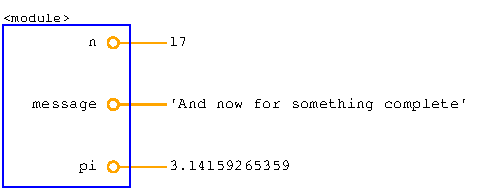
\includegraphics[scale = 0.7] {figs/lumpydemo1.pdf}}
\caption{Diagrama de estados gerada por Lumpy.}
\label{} fig.lumpy1
\end{figure}

Aqui está um exemplo que usa Lumpy para gerar um diagrama de estado.
\index{diagrama de estado} \index {estado diagrama!}

\begin{verbatim}
de swampy.Lumpy importação irregular

irregular = Lumpy ()
lumpy.make_reference ()

mensagem = 'E agora para algo completamente diferente'
n = 17
pi = 3,1415926535897932

lumpy.object_diagram ()
\end{verbatim}

A primeira linha importa a classe Lumpy de {\tt swampy.Lumpy}.
Se você não tem Swampy instalado como um pacote, certifique-se
os arquivos Swampy estão no caminho de busca do Python e usar este
{\tt importação} declaração em vez disso:

\begin{verbatim}
Lumpy de importação irregular
\end{verbatim}

As próximas linhas criar uma {\tt Lumpy} objeto e fazer um `` referência''
ponto, o que significa que Lumpy registra os objetos que foram
definido até agora.

Em seguida, definimos novas variáveis ​​e invocar \verb "object_diagram",
que atrai os objetos que foram definidos desde a referência
ponto, neste caso {mensagem tt \}, {\tt n} e {\tt pi}.

Figura ~ \ref {} fig.lumpy1 mostra o resultado. O estilo gráfico é
diferente do que eu mostrei mais cedo, por exemplo, cada
referência é representado por um círculo ao lado do nome da variável e um
A linha para o valor. E cadeias longas são truncadas. Mas o
informação transmitida pelo diagrama é o mesmo.

Os nomes de variáveis ​​estão em um quadro chamado \verbo "<module>", que
indica que estas são variáveis ​​em nível de módulo, também conhecidos como
global.
\index{variável global}
\index{variável! Mundial}
\index{variável de nível de módulo}
\index{variável! Em nível de módulo}

Você pode baixar este exemplo de
\url{http://thinkpython.com/code/lumpy_demo1.py}. Tente adicionar algumas
atribuições adicionais e ver o que o diagrama se parece.


\section{diagrama Stack}

\begin{figure}
\centerline
{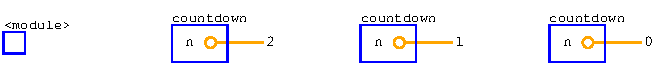
\includegraphics[scale = 0.7] {figs/lumpydemo2.pdf}}
\caption{diagrama Stack.}
\label{} fig.lumpy2
\end{figure}

Aqui está um exemplo que usa Lumpy para gerar um diagrama de pilha.
Você pode baixá-lo a partir de \url{http://thinkpython.com/code/lumpy_demo2.py}.
\index{diagrama de pilha} \index {diagrama! Empilhar}

\begin{verbatim}
de swampy.Lumpy importação irregular

contagem regressiva def (n):
    se n <= 0:
        imprimir 'Fogo!'
        lumpy.object_diagram ()
    else:
        print n
        contagem (n-1)

irregular = Lumpy ()
lumpy.make_reference ()
contagem regressiva (3)
\end{verbatim}

Figura ~ \ref {} fig.lumpy2 mostra o resultado. Cada quadro é representado
com uma caixa que tem o nome da função fora e variáveis ​​dentro.
Uma vez que esta função é recursivo, existe um quadro para cada
nível de recursão.
\index{recursão}
\index{função frame}
\index{frame}

Lembre-se que um diagrama de pilha mostra o estado do programa em
um determinado ponto em sua execução. Para obter o diagrama que você quiser,
às vezes você tem que pensar sobre onde a invocar \verb "object_diagram".

Neste caso, invoco \verb "object_diagram" depois de executar a base
caso da recursividade, dessa forma o diagrama de pilha mostra cada nível de
a recursão. Você pode chamar \verb "object_diagram" mais de uma vez para
obter uma série de instantâneos de execução do programa.
\index{caso base}


\{Diagramas de Objetos} secção

\begin{figure}
\centerline
{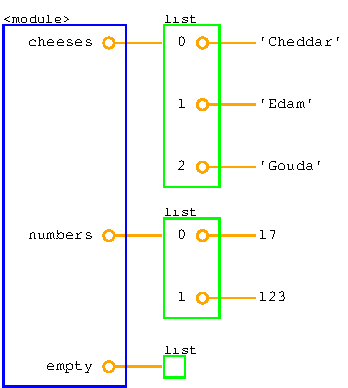
\includegraphics[scale = 0.7] {figs/lumpydemo3.pdf}}
\caption{diagrama de objeto.}
\label{} fig.lumpy3
\end{figure}

Este exemplo gera um diagrama de objetos mostrando as listas de
Seção ~ \ref {} seqüência. Você pode baixá-lo a partir de
\url{http://thinkpython.com/code/lumpy_demo3.py}.
\index{diagrama de objetos} \index {diagrama de objetos!}

\begin{verbatim}
de swampy.Lumpy importação irregular

irregular = Lumpy ()
lumpy.make_reference ()

queijos = ['Cheddar', 'Edam', 'Gouda']
Números = [17, 123]
= vazios []

lumpy.object_diagram ()
\end{verbatim}

Figura ~ \ref {} fig.lumpy3 mostra o resultado. Listas são representados por
uma caixa que mostra o mapeamento índices para os elementos. Esta representação
é um pouco enganador, uma vez que os índices não são realmente
parte da lista, mas eu acho que eles fazem o esquema mais fácil
ler. A lista vazia é representada por uma caixa vazia.
\{Index lista} índice

\begin{figure}
\centerline
{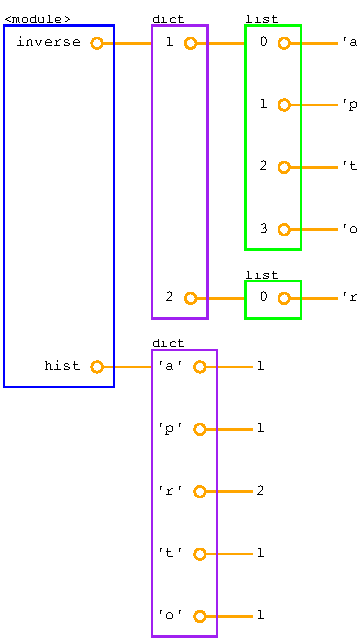
\includegraphics[scale = 0.7] {figs/lumpydemo4.pdf}}
\caption{diagrama de objeto.}
\label{} fig.lumpy4
\end{figure}

E aqui está um exemplo 
mostrando os dicionários da Seção ~ \ref {} invertido. Você pode baixar
isto a partir de \url{http://thinkpython.com/code/lumpy_demo4.py}.
\index{} dicionário

\begin{verbatim}
de swampy.Lumpy importação irregular

irregular = Lumpy ()
lumpy.make_reference ()

hist = histograma ('papagaio')
inverse = invert_dict (hist)

lumpy.object_diagram ()
\end{verbatim}

Figura ~ \ref {} fig.lumpy4 mostra o resultado. {\tt hist} é um dicionário
que mapeia a partir de caracteres (strings de uma letra) para inteiros;
{\tt inversa} mapeia a partir de números inteiros de listas de strings.

\begin{figure}
\centerline
{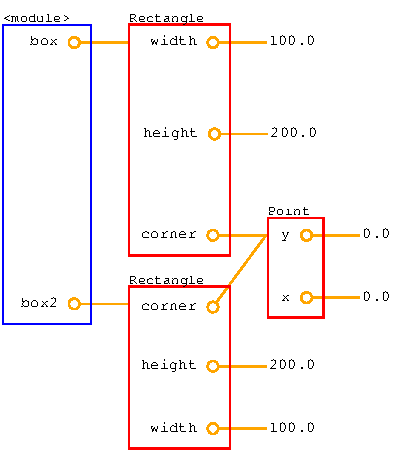
\includegraphics[scale = 0.7] {figs/lumpydemo5.pdf}}
\caption{diagrama de objeto.}
\label{} fig.lumpy5
\end{figure}

Este exemplo gera um diagrama de objetos para o Ponto e Retângulo
objetos, como na Seção ~ \ref {cópia}. Você pode baixá-lo a partir de
\url{http://thinkpython.com/code/lumpy_demo5.py}.
\{Classe Point} índice
\index{classe! Ponto}
\{Classe Retângulo} índice
\index{classe! Retângulo}

\begin{verbatim}
cópia de importação
de swampy.Lumpy importação irregular

irregular = Lumpy ()
lumpy.make_reference ()

box = Retângulo ()
box.width = 100,0
box.height = 200,0
box.corner = Ponto ()
box.corner.x = 0,0
box.corner.y = 0,0

box2 = copy.copy (box)

lumpy.object_diagram ()
\end{verbatim}

Figura ~ \ref {} fig.lumpy5 mostra o resultado. {\tt copy.copy} fazer uma
cópia superficial, então {caixa tt \} e {\tt box2} têm o seu próprio {width \tt}
e {\tt altura}, mas eles compartilham o mesmo objeto Point incorporado. Este
tipo de compartilhamento é geralmente muito bem com objetos imutáveis, mas com
tipos mutáveis, é altamente propenso erro.
\index{cópia}
\index{cópia superficial}

\section{função e classe objetos}

\begin{figure}
\centerline
{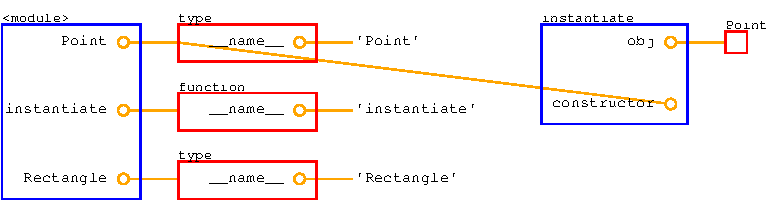
\includegraphics[scale = 0.7] {figs/lumpydemo6.pdf}}
\caption{diagrama de objeto.}
\label{} fig.lumpy6
\end{figure}

Quando eu uso irregular para fazer diagramas de objetos, eu costumo definir as funções
e as aulas antes de fazer o ponto de referência. Dessa forma, a função
e objetos de classe não aparecem no diagrama.
\index{função de objeto}
\index{objeto! Função}
\index{classe de objeto}
\index{objeto! Classe}

Mas se você está passando funções e classes como parâmetros, você pode
deseja que eles apareçam. Este exemplo mostra o que parece;
Você pode baixá-lo a partir de
\url{http://thinkpython.com/code/lumpy_demo6.py}.

\begin{verbatim}
cópia de importação
de swampy.Lumpy importação irregular

irregular = Lumpy ()
lumpy.make_reference ()

Ponto de classe (objeto):
    "" "Representa um ponto no espaço de 2-D." ""

classe Retângulo (object):
    "" "Representa um retângulo." ""

def instanciar (construtor):
    "" "Instancia um novo objeto." ""
    obj = construtor ()
    lumpy.object_diagram ()
    voltar obj

ponto = instanciar (Point)
\end{verbatim}

Figura ~ \ref {} fig.lumpy6 mostra o resultado. Desde que invocar
\Verb "object_diagram" dentro de uma função, temos um diagrama de pilha
com uma moldura para as variáveis ​​em nível de módulo e para a invocação
de {\tt instanciar}.

No nível de módulo, {\tt Ponto} e {\tt Retângulo} referem-se a
objetos de classe (que têm tipo {type \tt}); {\tt instanciar}
refere-se a um objeto de função.
\index{instanciar}
\index{construtor}

Este diagrama pode esclarecer dois pontos de confusão comum: (1) a
diferença entre o objeto de classe, {\tt Ponto}, ea instância do
Point, {\tt obj}, e (2) a diferença entre o objeto de função
criado quando {\tt instanciar} está definido, eo quadro criado com
ele é chamado.


\section{} diagramas de classes

\begin{figure}
\centerline
{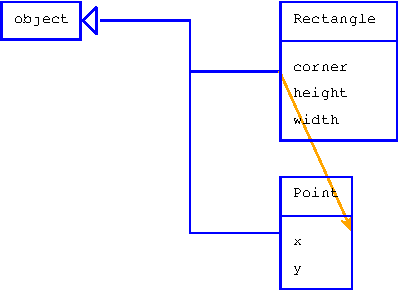
\includegraphics[scale = 0.7] {figs/lumpydemo7.pdf}}
\caption{Diagrama de Classe.}
\label{} fig.lumpy7
\end{figure}

\begin{figure}
\centerline
{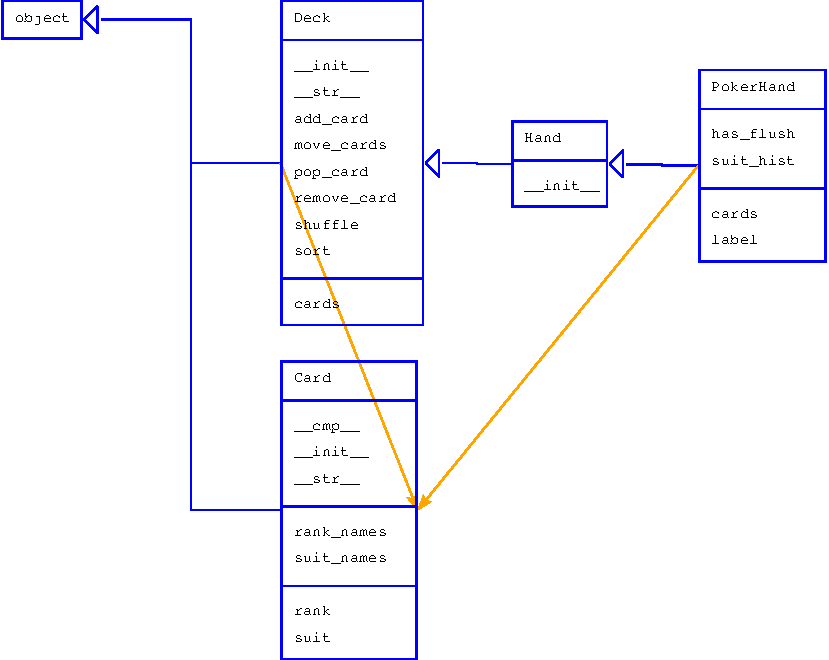
\includegraphics[scale = 0.7] {figs/lumpydemo8.pdf}}
\caption{Diagrama de Classe.}
\label{} fig.lumpy8
\end{figure}

Embora eu distinguir entre diagramas de estado, diagramas da pilha e
objeto diagramas, eles são praticamente a mesma coisa: eles mostram o
estado de um programa em execução em um ponto no tempo.
\{} Diagrama de classes do índice
\index{diagrama! Classe}

Os diagramas de classe são diferentes. Eles mostram as classes que compõem um
programa e as relações entre eles. Eles são atemporais no
sentido de que eles descrevem o programa como um todo, e não qualquer especial
ponto no tempo. Por exemplo, se uma instância da classe A geralmente
contém uma referência a uma instância da classe B, dizemos que há um
`` Tem-A relação'' entre essas classes.
\index{TEM-A relação}
\{} Diagrama de classes do índice
\index{diagrama! Classe}
\index{} UML

Aqui está um exemplo que mostra um tem-um relacionamento. Você pode baixar
isto a partir de \url{http://thinkpython.com/code/lumpy_demo7.py}.

\begin{verbatim}
de swampy.Lumpy importação irregular

irregular = Lumpy ()
lumpy.make_reference ()

box = Retângulo ()
box.width = 100,0
box.height = 200,0
box.corner = Ponto ()
box.corner.x = 0,0
box.corner.y = 0,0

lumpy.class_diagram ()
\end{verbatim}

Figura ~ \ref {} fig.lumpy7 mostra o resultado.  
Cada classe é representada com uma caixa que contém o nome do
classe, todos os métodos da classe oferece, todas as variáveis ​​de classe, e
todas as variáveis ​​de instância. Neste exemplo, {\tt Retângulo} e {Ponto \tt}
ter variáveis ​​de instância, mas não métodos ou variáveis ​​de classe.

A seta do {\tt Retângulo} para {\tt Ponto} mostra que retângulos
Ponto contêm um incorporado. Além disso, {\tt Retângulo} e {\tt
  Ponto} ambos herdam {\tt} objeto, que é representada em
o diagrama com uma seta com cabeça de triângulo.
\index{IS-A relação}

Aqui está um exemplo mais complexo usando a minha solução para o Exercício ~ \ref {} de poker.
Você pode baixar
o código de \url{http://thinkpython.com/code/lumpy_demo8.py};
você também vai precisar \url{http://thinkpython.com/code/PokerHand.py}.

\begin{verbatim}
de swampy.Lumpy importação irregular

de Pokerhand import *

irregular = Lumpy ()
lumpy.make_reference ()

convés = Deck ()
mão = Pokerhand ()
deck.move_cards (mão, 7)

lumpy.class_diagram ()
\end{verbatim}

Figura ~ \ref {} fig.lumpy8 mostra o resultado.  
{\tt Pokerhand} herda {\tt Mão}, que herda de {\tt plataforma}.
Ambos {\tt plataforma} e {\tt Pokerhand} tem Cards.
\{Classe} Cartão índice
\index{classe Baralho}
\index{classe Mão}

Este diagrama não mostra que {\tt Mão} também tem cartões, porque
no programa não há casos de Hand. Este exemplo
demonstra uma limitação de Lumpy, só sabe sobre o
atributos e relacionamentos tem-um dos objetos que são instanciados.

\Printindex

\Clearemptydoublepage
%\blankpage
%\blankpage
%\blankpage


\end{document}
